% !TEX root = ./thesis.tex
% SETTINGS

%!TEX root = ../thesis.tex
\RequirePackage{fix-cm} % against warnings for \fontsize
\documentclass[a4paper,12pt,numbers=noenddot,listof=entryprefix,usegeometry,open=right,headings=big,pairskip=half]{scrreprt}

\usepackage{amsmath}
\usepackage{amssymb}
\usepackage{physics} % for \abs, \dd, ...
%\usepackage{siunitx} % for \micro, \SI
\usepackage{slashed}
\usepackage[T1]{fontenc} % load before inputenc
\usepackage[utf8]{inputenc}
\usepackage[scaled]{helvet}
\usepackage[english]{babel}
\usepackage{xifthen} % for \ifthenelse, \isempty
\usepackage{xspace} % for \xspace in macros
\usepackage{lipsum}
\usepackage{graphicx, caption}
\usepackage{subcaption,float}
\usepackage{amssymb}
\usepackage{algorithm}
\usepackage{algpseudocode}
%\counterwithout*{footnote}{chapter}
%\usepackage{tikz}
%\usetikzlibrary{calc,positioning,shadows.blur,decorations.pathreplacing}
%\usepackage{etoolbox}

%%%% MATRIX
%%%\usepackage{kbordermatrix}
%%%\renewcommand{\kbldelim}{(}
%%%\renewcommand{\kbrdelim}{)}

% FIGURES
\usepackage{graphicx} %[pdftex],graphics
\usepackage{subfig} % conflicts with tocloft
%\let\subfigure\subfloat% compatibility between subfigure and subfig packages
\usepackage[format=plain,labelfont=bf,skip=6pt]{caption}
%\usepackage{capt-of}
%\usepackage{qtree}
%\usepackage{wrapfig} % to wrap text around figure
\usepackage[hang,flushmargin]{footmisc} % force footnotes below floats %add perpage to reset counter each page
\usepackage{etoolbox}

% Make custom counter for the footnotes
% Patch the footnote command to bend to our needs
\patchcmd{\footnote}{\@mpfn}{{myfootnote}}\relax\relax
\patchcmd{\footnote}{\thempfn}{{\themyfootnote}}\relax\relax



%%% FIGURES numbering
%%%\newcounter{myfigure}
%%%\renewcommand{\thefigure}{\arabic{myfigure}}
%%%\newcounter{mytable}
%%%\renewcommand{\thetable}{\arabic{mytable}}
%%%\usepackage{makeidx} \makeindex
%%%\makeglossary

% TABLE
\usepackage[table]{xcolor}
\usepackage{multirow}
%\usepackage{booktabs} % more options for table shapes
%\usepackage{topcapt} % for \topcaption
\newcommand{\topcaption}[1]{\caption{#1}} % dummy
%\usepackage{floatrow} % to put table and figure side-by-side
%%%\newfloatcommand{capbtabbox}{table}[][\FBwidth]
%%%\DeclareFloatVCode{beforefloat}{\vspace{2pt}}
%%%\DeclareFloatVCode{afterfloat}{\vspace{-10pt}}
%%%\floatsetup[table]{capposition=top,captionskip=0pt} %,precode=beforefloat,postcode=afterfloat
%%%\usepackage{cellspace} % for \cellspacetoplimit, \cellspacebottomlimit
%%%\setlength\cellspacetoplimit{100pt}
%%%\setlength\cellspacebottomlimit{100pt}

% FLOAT SPACING
% https://tex.stackexchange.com/questions/23313/how-can-i-reduce-padding-after-figure
\setlength{\floatsep}{8pt plus 3pt minus 3pt} % space left between floats 
\setlength{\textfloatsep}{9pt plus 3pt minus 3pt} % space between last top float or first bottom float and the text
\setlength{\abovecaptionskip}{2pt plus 2pt minus 2pt} % vertical space between caption & fig
\setlength{\belowcaptionskip}{2pt plus 2pt minus 2pt} % vertical space between caption & fig

%%% PDF
%%%\usepackage{pdfpages} % for \includepdf for title page (load after table package)
%%%\usepackage{tikz} % for drawing, load after multirow to avoid conflict

% REFERENCES
\usepackage[square,numbers,sort&compress]{natbib} % more options for citations, e.g. square brackets
\renewcommand{\bibsection}{}
%\setlength{\bibitemsep}{10pt} % bibtex
\setlength{\bibsep}{0.5\baselineskip} % natbib

% METADATA
\definecolor{myblue}{RGB}{0,82,155}

\usepackage[hyperfootnotes=true,linktoc=all]{hyperref} % for url hyperlinks; load last to prevent problems %,pagebackref=true
\hypersetup{%
  pdfauthor={Piero Viscone},
  pdftitle={Measurement of the $V_{cb}$ CKM element from $t\bar{t}$ semileptonic decays at CMS},
  pdfsubject={Piero Viscone master thesis - Measurement of the $V_{cb}$ CKM element from $t\bar{t}$ semileptonic decays at CMS},
  pdfkeywords={},
  %pdfborder={111}, % for hyperlinks in pdf
  colorlinks=true,
  linkcolor={},
  citecolor={red!80!black},
  %urlcolor={blue!80!black}
}

%%%% FEYNMAN FIGURES
%%%\usepackage{feynmp}
%%%\DeclareGraphicsRule{*}{mps}{*}{}
%%%\makeatletter
%%%\def\endfmffile{
%%%  \fmfcmd{\p@rcent\space the end.^^J end.^^J endinput;}
%%%  \if@fmfio
%%%    \immediate\closeout\@outfmf
%%%  \fi
%%%  %\ifnum\pdfshellescape=\@ne
%%%  \ifnum\pdfshellescape>\z@
%%%    \immediate\write18{mpost \thefmffile}
%%%  \fi}
%%%\makeatother

%%% TOC % does not work well with the KOMA class (scrreprt)
%%\usepackage[subfigure,titles]{tocloft}
%%\setlength{\cftbeforechapskip}{0.8em}
%%%\setlength{\cftbeforechapskip}{0.8em}
%%\setlength{\cftsecindent}{1.6em}
%%\setlength{\cftsecnumwidth}{2.6em}
%%\setlength{\cftsubsecindent}{4.2em}
%%\setlength{\cftsubsecnumwidth}{3.0em}
%%\setlength{\cftsubsubsecindent}{4.5em}
%%\setlength{\cftsubsubsecnumwidth}{4em}

% PAGE LAYOUT & MARGINS
\usepackage{geometry} % WARNING: add 'usegeometry' option to \documentclass for scrreprt class
\setlength{\topmargin}{-1.2cm}
%\setlength{\bottommargin}{-1.2cm}
\setlength{\oddsidemargin}{0.2cm}
\setlength{\evensidemargin}{0.2cm}
\setlength{\textheight}{25cm}
\setlength{\textwidth}{16cm}
\setlength{\footskip}{1.2cm} 
\setlength{\footnotesep}{0.4cm}

%%%% HEADER & FOOTER

\usepackage[chapterstyle=bianchi,headings=big]{settings/komaChapStyle}
\usepackage{bm}
\usepackage{fancyhdr}
\pagestyle{fancy}
\fancyhf{}

\lhead{\nouppercase{\textbf{\rightmark}}}
\rhead{\textbf{\thepage}}
\fancyfoot{}


%\usepackage{fancyhdr}
%\pagestyle{fancy} 
%\fancyhf{}
%%%
%%%% Lines after a header or before a footer
%%%%\renewcommand{\footrulewidth}{0.4pt}
%%%\renewcommand{\headrulewidth}{0.4pt}
%%%
%%%\fancyhead[L]{\footnotesize{\leftmark}}
%%%\fancyhead[R]{}
%%%\fancyfoot[C]{\footnotesize{\thepage}}
%%%
%%%% Plain pagestyle for first chapter page
%%%\fancypagestyle{plain}{%
%%%  \fancyhf{} 
%%%  \renewcommand{\headrulewidth}{0pt}
%%%  \fancyfoot[C]{\footnotesize{\thepage}}
%%%}

% PARAGRAPH SPACING
\parskip=0cm
\parindent=0.5cm

% LINE SPACING
\usepackage{lineno} % line numbers
\usepackage[nodisplayskipstretch]{setspace}
%\onehalfspacing %\doublespace or \singlespace
\setstretch{1.09}
%\setdisplayskipstretch{1} % override \setstretch for equations
%\linespread{1.15} % without setspace package

% EQUATIONS SPACING
\AtBeginDocument{%
 \setlength{\belowdisplayskip}{9pt}%
 \setlength{\belowdisplayshortskip}{9pt}%
 \setlength{\abovedisplayskip}{9pt}%
 \setlength{\abovedisplayshortskip}{9pt}%
}

% BOLD MATH in section titles
% https://tex.stackexchange.com/questions/41379/automatically-typeset-math-in-section-headings-in-bold-face
\makeatletter
\g@addto@macro\bfseries{\boldmath}
\makeatother

% CHAPTER NUMBERING macro
\newcommand{\newchap}[1]{
  \chapter{#1}
  \markboth {Chapter \thechapter.  {#1}}{Chapter \thechapter.  {#1}}
}

% NUMBERING LEVEL
\setcounter{secnumdepth}{4}
\setcounter{tocdepth}{2}
%\setcounter{lofdepth}{1} 

% FOOTNOTES
\newcounter{myfootnote}[chapter]
\renewcommand{\thefootnote}{\themyfootnote}
\newcommand{\myfootnote}[1]{\stepcounter{myfootnote}\footnote{#1}}


% LISTS (itemize, enumerate) spacing
\usepackage{enumitem}
\setlist[enumerate]{itemsep=0pt,topsep=6pt}
\setitemize{itemsep=0pt,topsep=6pt}
%%%\renewenvironment{itemize}%
%%%  {\begin{list}{$\bullet$}{%
%%%    \setlength{\topsep}{5pt}%
%%%    %\setlength{\botsep}{5pt}%
%%%    \setlength{\partopsep}{2pt}%
%%%    \setlength{\parsep}{0.5\parskip}%
%%%    \setlength{\itemsep}{2pt}%
%%%    \setlength{\leftmargin}{7ex}%
%%%    \setlength{\rightmargin}{3ex}%
%%%  }}{\end{list}}%

%Change the bullet in itemize
\usepackage{pifont}
\renewcommand\labelitemi{\ding{228}}


% Minitoc
\usepackage{minitoc}


\mtcsettitle{minitoc}{}
%spacing minitoc
\renewcommand{\kernafterminitoc}{\kern0.5\baselineskip\kern0ex}


% Colors
\definecolor{myblue}{RGB}{0,82,155}
\renewcommand{\familydefault}{\rmdefault}
\addtokomafont{chapter}{\normalfont\huge\bfseries}
\addtokomafont{section}{\normalfont\bfseries}
%\addtokomafont{subsection}{}
%\addtokomafont{subsubsection}{}
\addtokomafont{chapterentry}{\normalfont\bfseries}
\setkomafont{subsubsection}{\fontsize{13}{15}\selectfont}
%!TEX root = ../thesis.tex
% Author: Izaak Neutelings (February 2023)
% Description: Mimicking common CMS TDR macros & particle pennames
% Sources:
%   https://gitlab.cern.ch/tdr/utils/-/blob/master/general/hepparticles.sty
%   https://gitlab.cern.ch/tdr/utils/-/blob/master/general/heppennames2.sty
%   https://gitlab.cern.ch/tdr/utils/-/blob/master/general/ptdr-definitions.sty

% CMS TDR: text
\newcommand{\etal}   {\mbox{et al.}\xspace} %et al. - no preceding comma
\newcommand{\ie}     {\mbox{i.e.}\xspace}
\newcommand{\eg}     {\mbox{e.g.}\xspace}
\newcommand{\etc}    {\mbox{etc.}\xspace}

% CMS TDR: common macros
\newcommand{\PNfix}   {\hspace{-.04em}}
\newcommand*{\DOI}[1]{\href{http://dx.doi.org/#1}{\texttt{doi:#1}}} % CHECK REFERENCE 10.1103 !!!
\providecommand{\NA}{\ensuremath{\text{---}}}
\providecommand{\cmsTable}[1]{\resizebox{\textwidth}{!}{#1}}

% CMS TDR: units
%\newcommand{\unit}[1]{{\ensuremath{\text{\,#1}}}\xspace}
\newcommand{\mus}    {{\ensuremath{\,\text{\textmu s}}}\xspace} %\upmu
\newcommand{\mum}    {{\ensuremath{\,\text{\textmu m}}}\xspace}
\newcommand{\cm}     {{\ensuremath{\,\text{cm}}}\xspace}
\newcommand{\MeV}    {{\ensuremath{\,\text{Me\hspace{-.08em}V}}}\xspace}
\newcommand{\GeV}    {{\ensuremath{\,\text{Ge\hspace{-.08em}V}}}\xspace}
\newcommand{\TeV}    {{\ensuremath{\,\text{Te\hspace{-.08em}V}}}\xspace}
\newcommand{\fbinv}  {{\mbox{\ensuremath{\,\text{fb}^\text{$-$1}}}}\xspace}

% CMS TDR: SOFTWARE PROGRAMS
\newcommand{\GEANTfour} {{\textsc{Geant4}}\xspace}
\newcommand{\GEANTthree} {{\textsc{geant3}}\xspace}
\newcommand{\GEANT} {{\textsc{geant}}\xspace}
\newcommand{\FASTJET} {{\textsc{FastJet}}\xspace}
\newcommand{\FEWZ} {{\textsc{fewz}}\xspace}
\newcommand{\Toppp} {\textsc{Top$++$}\xspace}
\newcommand{\HERWIG} {{\textsc{herwig}}\xspace}
\newcommand{\PYTHIA} {{\textsc{pythia}}\xspace}
\newcommand{\MADGRAPH} {\textsc{MadGraph}\xspace}
\newcommand{\MADSPIN} {\textsc{MadSpin}\xspace}
\newcommand{\MLM} {\textsc{MLM}\xspace}
\newcommand{\FXFX} {\textsc{FxFx}\xspace}
\newcommand{\aMCATNLO}{a\textsc{mc@nlo}\xspace}
\newcommand{\MCATNLO} {\textsc{mc@nlo}\xspace}
\newcommand{\MGvATNLO}{\MADGRAPH{}5\_a\MCATNLO}
\newcommand{\POWHEG} {{\textsc{powheg}}\xspace}
\newcommand{\TAUOLA} {\textsc{tauola}\xspace}
\newcommand{\DeepTau} {{\textsc{DeepTau}}\xspace}
\newcommand{\DeepCSV} {{\textsc{DeepCSV}}\xspace}
\newcommand{\DeepJet} {{\textsc{DeepJet}}\xspace}
\newcommand{\Djet}{\ensuremath{D_\text{jet}}\xspace} % DeepJet
\newcommand{\DeepTauVSe}{\texttt{DeepTau2017v2p1VSe}\xspace}
\newcommand{\DeepTauVSmu}{\texttt{DeepTau2017v2p1VSmu}\xspace}
\newcommand{\DeepTauVSjet}{\texttt{DeepTau2017v2p1VSjet}\xspace}

% CMS TDR PARTICLE PENNAMES
% https://gitlab.cern.ch/tdr/utils/-/blob/master/general/heppennames2.sty
% grep '\\PZ' */*.tex *.tex
% sed -e 's/\\PZ/\\PZ/g' -i '' *.tex */*.tex # macOS
% https://mirror.foobar.to/CTAN/macros/latex/contrib/was/upgreek.pdf
% https://ctan.org/pkg/fntguide

% UNSLANT small greek letters to make them look straight for particle names
% https://tex.stackexchange.com/questions/145926/upright-greek-font-fitting-to-computer-modern
% https://tex.stackexchange.com/questions/236915/adjust-custom-made-upright-greek-letters-when-used-in-subscripts
\usepackage{scalerel}
\newsavebox{\foobox}
\newcommand{\slantbox}[2][0]{\mbox{%
        \sbox{\foobox}{#2}%
        \hskip\wd\foobox
        \pdfsave
        \pdfsetmatrix{1 0 #1 1}%
        \llap{\usebox{\foobox}}%
        \pdfrestore
}}
\newcommand\unslant[2][-.25]{%
  \mkern1.2mu%
  \ThisStyle{\slantbox[#1]{$\SavedStyle#2$}}%
  \mkern-1.2mu%
}
\newcommand\unslantlong[2][-.25]{% % for long letter like mus
  \mkern-0.2mu%
  \ThisStyle{\slantbox[#1]{$\SavedStyle#2$}}%
  \mkern-0.8mu%
}
\newcommand{\upalpha}{\unslant\alpha}
\newcommand{\upgamma}{\unslant\gamma}
\newcommand{\upeta}{\unslant\eta}
\newcommand{\upmu}{\unslantlong\mu}
\newcommand{\upnu}{\unslant\nu}
\newcommand{\uppi}{\unslant\pi}
\newcommand{\uprho}{\unslant\rho}
\newcommand{\uptau}{\unslant\tau}
\newcommand{\upphi}{\unslantlong\phi}
\newcommand{\upchi}{\unslantlong\chi}
\newcommand{\uppsi}{\unslant\psi}
\newcommand{\upomega}{\unslant\omega}

% CMS TDR: PENNAMES
% https://gitlab.cern.ch/tdr/utils/-/blob/master/general/heppennames2.sty
\newcommand{\Pl}{{\ensuremath{\ell}}\xspace}
\newcommand{\PAl}{{\ensuremath{\overline{\ell}}}\xspace}
\newcommand{\Pe}{{\ensuremath{\text{e}}}\xspace} % electron
\newcommand{\PGm}{{\ensuremath{\upmu}}\xspace} % muon
\newcommand{\PGt}{{\ensuremath{\uptau}}\xspace}
\newcommand{\PGn}{{\ensuremath{\upnu}}\xspace}
\newcommand{\PGnl}{{\ensuremath{\upnu_{\ell}}}\xspace}
\newcommand{\PGne}{{\ensuremath{\upnu_{\Pe}}}\xspace}
\newcommand{\PGnGm}{{\ensuremath{\upnu_{\PGm\mkern-0.9mu}}}\xspace}
\newcommand{\PGnGt}{{\ensuremath{\upnu_{\PGt\mkern-0.9mu}}}\xspace}
\newcommand{\PAGnl}{{\ensuremath{\overline\upnu_{\ell}}}\xspace} % anti-neutrino
\newcommand{\PAGne}{{\ensuremath{\overline\upnu_{\Pe}}}\xspace}
\newcommand{\PAGnGm}{{\ensuremath{\overline\upnu_{\PGm\mkern-.9mu}}}\xspace}
\newcommand{\PAGnGt}{{\ensuremath{\overline\upnu_{\PGt\mkern-.9mu}}}\xspace}
\newcommand{\PQu}{{\ensuremath{\text{u}}}\xspace} % for u quark
\newcommand{\PQd}{{\ensuremath{\text{d}}}\xspace} % for d quark
\newcommand{\PQc}{{\ensuremath{\text{c}}}\xspace} % for c quark
\newcommand{\PQs}{{\ensuremath{\text{s}}}\xspace} % for s quark
\newcommand{\PQt}{{\ensuremath{\text{t}}}\xspace} % for t quark
\newcommand{\PQb}{{\ensuremath{\text{b}}}\xspace} % for b quark
\newcommand{\PAQu}{{\ensuremath{\bar{\text{u}}}}\xspace} % for u antiquark
\newcommand{\PAQd}{{\ensuremath{\bar{\text{d}}}}\xspace} % for d antiquark
\newcommand{\PAQc}{{\ensuremath{\bar{\text{c}}}}\xspace} % for c antiquark
\newcommand{\PAQs}{{\ensuremath{\bar{\text{s}}}}\xspace} % for s antiquark
\newcommand{\PAQt}{{\ensuremath{\bar{\text{t}}}}\xspace} % for t antiquark
\newcommand{\PAQb}{{\ensuremath{\bar{\text{b}}}}\xspace} % for b antiquark
\newcommand{\PQq}{{\ensuremath{q}}\xspace} % generic quark
\newcommand{\PGg}{{\ensuremath{\gamma}}\xspace} % photon (gamma)
\newcommand{\Pg}{{\ensuremath{g}}\xspace} % generic gluon
\newcommand{\PW}{{\ensuremath{\text{W}}}\xspace} % W boson
\newcommand{\PZ}{{\ensuremath{\text{Z}}}\xspace} % Z boson
\newcommand{\PH}{{\ensuremath{\text{H}}}\xspace} % Higgs boson
\newcommand{\Zg}{{\ensuremath{\PZ\kern-0.5pt/\kern-0.5pt\gamma^*}}\xspace} % photon / Z
\newcommand{\PGp}{\ensuremath{\uppi}\xspace} % pion
\newcommand{\PGr}{\ensuremath{\uprho}\xspace} % rho
\newcommand{\Pa}{\ensuremath{\text{a}}\xspace} % a_1
\newcommand{\PK}{\ensuremath{\mathrm{K}}\xspace} % kaon
\newcommand{\PAK}{\ensuremath{\overline{\mathrm{K}}}\xspace} % kaon
\newcommand{\Pp}{\ensuremath{\mathrm{p}}\xspace} % proton
\newcommand{\Pn}{\ensuremath{\mathrm{n}}\xspace} % neutron
\newcommand{\PD}{\ensuremath{\mathrm{D}}\xspace} % D meson
\newcommand{\PB}{\ensuremath{\mathrm{B}}\xspace} % B meson
\newcommand{\PAB}{\ensuremath{\overline{\mathrm{B}}}\xspace} % B meson
\newcommand{\PJGy}{\ensuremath{\mathrm{J}\mspace{-2mu}/\mspace{-2mu}\uppsi}\xspace} %  J/psi meson
\newcommand{\PGU}{\ensuremath{\Upsilon}\xspace} % Upsilon

% CMS TDR: common particle combinations
\newcommand{\bsln} {\ensuremath{\PQb\to\PQc\ell\PAGnl}\xspace} % b -> c ell nu
\newcommand{\bstn} {\ensuremath{\PQb\to\PQc\PGt\PGnGt}\xspace} % b -> s tau nu
\newcommand{\ttbar}{{\ensuremath{\PQt\PAQt}}\xspace}
\newcommand{\bbbar}{{\ensuremath{\PQb\PAQb}}\xspace}
\newcommand{\EE}   {{\ensuremath{\Pe^+\Pe^-}}\xspace}
\newcommand{\MM}   {{\ensuremath{\PGm^+\PGm^-}}\xspace}
\newcommand{\TT}   {{\ensuremath{\PGt^+\PGt^-}}\xspace}
\newcommand{\LL}   {{\ensuremath{\ell^+\ell^-}}\xspace}

% CMS TDR: common particle physics symbols
\newcommand{\lumi}   {{\ensuremath{\mathcal{L}}}\xspace}
\newcommand{\DR}     {{\ensuremath{\Delta R}}\xspace}
\newcommand{\ET}     {\ensuremath{E_\text{T}}\xspace}
\newcommand{\kt}     {\ensuremath{k_\text{T}}\xspace}
\newcommand{\pt}     {\ensuremath{p_\text{T}}\xspace}
\newcommand{\ptvec}  {{\ensuremath{\myvec{p}_\text{T}}}\xspace}
\newcommand{\ptmiss} {\ensuremath{\pt^\text{miss}}\xspace}
\newcommand{\ptvecmiss}{\ensuremath{{\myvec{p}}_{\mathrm{T}}^{\kern1pt\text{miss}}}\xspace}
\newcommand{\ptvecvis}[1][]{\ensuremath{{\myvec{p}}_{\mathrm{T}\ifthenelse{\isempty{#1}}{}{,#1}}^{\kern1pt\text{vis}}}\xspace}
\newcommand{\MET}    {{\ensuremath{\text{MET}}}\xspace}
\newcommand{\ETmiss} {{\ensuremath{E_{\mathrm{T}}^{\text{miss}}}}\xspace}
\newcommand{\PT}     {\pt}
\newcommand{\mT}     {{\ensuremath{m_\text{T}}}\xspace}
 % CMS TDR macros & particle pennames
%!TEX root = ../thesis.tex
% Author: Izaak Neutelings (February 2023)
% Description: My common macros

% IWN: text
\newcommand\TODO[1]  {\textsf{({\color{blue!60!black!40}\textbf{TODO}: #1})}\xspace}
\newcommand\ADDREF   {\textsf{\color{blue!60!black!40}\textbf{\small[add Ref.]}}\xspace}
\newcommand\FIXME[1] {\textsf{(\textbf{FIXME}: #1)}}
\newcommand{\Left}   {\textbf{Left}}
\newcommand{\Middle} {\textbf{Middle}}
\newcommand{\Right}  {\textbf{Right}}
\newcommand{\Top}    {\textbf{Top}}
\newcommand{\Bottom} {\textbf{Bottom}}
\newcommand{\Fig}[1] {Fig.~\ref{#1}\xspace}
\newcommand{\Eq}[1]  {Eq.~\eqref{#1}\xspace}
\newcommand{\tabsubtitle}[1]{\rule{0pt}{13pt}\textbf{#1}} % subtitle in table
\newcommand{\phmin}  {\phantom{-}} % for aligning pos/neg. values in centered columns
\newcommand*{\myvec}[1]{\vec{\mkern0mu#1}} % correct misalignment in \vec
\newcommand*{\defeq}{\mathrel{\vcenter{\baselineskip0.5ex \lineskiplimit0pt
                     \hbox{\scriptsize.}\hbox{\scriptsize.}}}=} % definition :=

% IWN: Standard Model
\newcommand{\Lg}[1]  {\mathcal{L}_\text{#1}} % Lagrangian
\newcommand{\ff}[2]{#1_\text{#2}} % fermion field
\newcommand{\aff}[2]{\overline{#1}\vphantom{#1}_\text{#2}} % anti-fermion field
\newcommand{\U}[2][]{\text{U}(#2)\ifthenelse{\isempty{#1}}{}{_\text{#1}}} % U(N)
\newcommand{\SU}[2][]{\text{SU}(#2)\ifthenelse{\isempty{#1}}{}{_\text{#1}}} % SU(N)
\newcommand{\GSM}    {{\ensuremath{\SU[C]{3}\times\SU[L]{2}\times\U[Y]{1}}}\xspace} % SM group
\newcommand{\Ggauge} {{\ensuremath{G_\mathrm{gauge}^\mathrm{global}}}\xspace}
\newcommand{\YW}     {{\ensuremath{Y}}\xspace} % weak hypercharge %_\text{W}
\newcommand{\JW}     {\ensuremath{J_\mathrm{W}}\xspace} % charged weak current
\newcommand{\thetaW} {{\ensuremath{\theta_\mathrm{W}}}\xspace} % Weinberg mixing angle
\newcommand{\thetaC} {{\ensuremath{\theta_\mathrm{C}}}\xspace} % Cabibbo mixing angle
\newcommand{\VCKM}   {\ensuremath{V_\mathrm{CKM}}\xspace} % CKM matrix
\newcommand{\CKM}   {\ensuremath{\mathrm{CKM}}\xspace}
\newcommand{\CMS}   {\ensuremath{\mathrm{CMS}}\xspace}
\newcommand{\GF}     {\ensuremath{G_\mathrm{F}}\xspace} % Fermi constant
\newcommand{\MW}     {\ensuremath{M_{\PW}}\xspace} % W boson mass
\newcommand{\MZ}     {\ensuremath{M_{\PZ}}\xspace} % Z boson mass
\newcommand{\db}[2]  {{\ensuremath{\def\arraystretch{1}\begin{pmatrix}#1\\#2\end{pmatrix}}}\xspace} % doublet
\newcommand{\tb}[3]  {{\ensuremath{\def\arraystretch{1}\begin{pmatrix}#1\\#2\\#3\end{pmatrix}}}\xspace} % doublet
\newcommand{\C}      {\ensuremath{{C}}} % charge conjugate
\newcommand{\Par}      {\ensuremath{{P}}} % charge conjugate
\newcommand{\CP}      {\ensuremath{{CP}}} % charge conjugate
\newcommand{\hc}     {{\ensuremath{\text{h.c.}}}\xspace} % hermitian conjugate

% IWN: common particles / final states
\newcommand{\tauh}   {{\ensuremath{\PGt\kern-0.5pt_\text{h}}}\xspace} % hadronic tau
\providecommand{\tt} {} % create dummy to prevent "undefined" error in OverLeaf
\renewcommand{\tt}   {{\ensuremath{\PGt\PGt}\xspace}}
\renewcommand{\ll}   {{\ensuremath{\ell\ell'}}\xspace}
\newcommand{\ee}     {{\ensuremath{\Pe\Pe}}\xspace}
\newcommand{\mumu}   {{\ensuremath{\PGm\PGm}}\xspace}
\newcommand{\emu}    {{\ensuremath{\Pe\PGm}}\xspace}
\newcommand{\ltau}   {{\ensuremath{\ell\tauh}}\xspace}
\newcommand{\etau}   {{\ensuremath{\Pe\tauh}}\xspace}
\newcommand{\mutau}  {{\ensuremath{\PGm\tauh}}\xspace}
\newcommand{\tautau} {{\ensuremath{\PGt\kern-0.2pt\PGt}}\xspace}
\newcommand{\ditau}  {{\ensuremath{\tauh\kern-0.5pt\tauh}}\xspace}
\newcommand{\btau}   {{\ensuremath{\PQb\PGt}}\xspace}
\newcommand{\LQ}     {{\ensuremath{\mathrm{LQ}}}\xspace}
\newcommand{\ALQ}    {{\ensuremath{\overline{\mathrm{LQ}}}}\xspace}
\newcommand{\Zjets}  {{\ensuremath{\PZ\PNfix+\text{jets}}\xspace}}
\newcommand{\Wjets}  {{\ensuremath{\PW\PNfix+\text{jets}}\xspace}}
\newcommand{\jtf}    {{\ensuremath{j\to\tauh}\xspace}}
\newcommand{\ltf}    {{\ensuremath{\ell\to\tauh}\xspace}}

% IWN: common variables
\newcommand{\BF}     {{\ensuremath{\mathcal{B}}}} % branching fraction
\newcommand{\ST}     {{\ensuremath{S_\mathrm{T}}}\xspace} % scalar-sum pt
\newcommand{\muR}    {{\ensuremath{\mu_\text{R}}\xspace}} % renormalization scale
\newcommand{\muF}    {{\ensuremath{\mu_\text{F}}\xspace}} % factorization scale
\newcommand{\mvis}   {{\ensuremath{m_\text{vis}}}\xspace} % visible mass
\newcommand{\mll}    {{\ensuremath{m_{\ell\ell}}}\xspace}
\newcommand{\mtauh}  {\ensuremath{m_{\tauh}}\xspace} % tau_h mass
\newcommand{\mLQ}    {{\ensuremath{m_{\LQ}}}\xspace}
\newcommand{\Irel}   {\ensuremath{I_\text{rel}}} % relative isolation
\newcommand{\Njets}  {\ensuremath{N_\text{jets}}\xspace}

% IWN: Statistics
\newcommand{\DNLL}{{\ensuremath{-2\Delta\kern-1.3pt\ln\kern-1.2pt\mathcal{L}}}\xspace}
\newcommand{\CL}{\ensuremath{\text{CL}}\xspace} % needs to be overridden to C.L. for APS. Look out for \CL.
\newcommand{\CLs}{\ensuremath{\text{CL}_\text{s}}\xspace}
\newcommand{\CLsb}{\ensuremath{\text{CL}_\text{s+b}}\xspace}

 % user commands

\begin{document}
\dominitoc
\emergencystretch 3em 
% TITLE PAGE
\pagenumbering{roman}
\begin{titlepage} %crea l'enviroment
    \begin{figure}[h!] %inserisce le figure
        \centering
\includegraphics[width=0.94\textwidth]{fig/Frontespizio/marchio_unipi_pant541.png}
    \end{figure}
    
    \vspace{10mm}
    
    \begin{Large}
     \begin{center}
        \textbf{Dipartimento di Fisica\\ Corso di Laurea Magistrale in Fisica\\}
        \vspace{20mm}
        {    {\Huge{\textbf{Measurement of the $V_{cb}$ \CKM element from \ttbar semileptonic \\ \vspace{3mm} decays at \CMS} }}}\\
    \end{center}
    \end{Large}
    
    
    \vspace{28mm}
    %minipage divide la pagina in due sezioni settabili
    \begin{minipage}[t]{0.47\textwidth}
        {\large{\textbf {Relatore:\\ Paolo Azzurri}}}
    \end{minipage}
    \hfill
    \begin{minipage}[t]{0.47\textwidth}\raggedleft
        {\large{\textbf {Candidato:\\ Piero Viscone}}}
    \end{minipage}
    
    \vspace{28mm}
    
    \hrulefill
    
    \vspace{5mm}
    
    \centering{\large{\textbf {Anno Accademico 2022/2023 }}}
    
    \end{titlepage}
 

\TODO{\Huge Gli istogrammi che pensavi fossero stackati, non sono stackati}

\linenumbers %! for review (remove in final version!)

% ABSTRACT & ACKNOWLEDGEMENTS
%!TEX root = ../thesis.tex
% UZH MNF only requires an English abstract. No German abstract or summary is required!
% See "fact sheet": https://www.mnf.uzh.ch/en/studium/phd/checkliste-fuer-doktorierende.html
 % force empty page (left-hand side) between abstract and acknowledgements
\thispagestyle{empty} % no page number
\newpage
\phantomsection % to get the hyperlinks (and bookmarks in PDF) right for index, list of files, bibliography, etc.
%\addcontentsline{toc}{chapter}{Abstract} % add to table of contents
%\begin{abstract}
%\section*{Abstract}

%\lipsum[1-2]

%\addcontentsline{toc}{chapter}{Summary}
%\section*{Summary}
%Here is a longer summary of the thesis.

%\end{abstract}
\addcontentsline{toc}{chapter}{Abstract} % add to table of contents
\begin{abstract}
\section*{Abstract}
The precise determination of the $|V_{cb}|$ Cabibbo-Kobayashi-Maskawa (CKM) element is of great interest as it currently is the CKM element with the largest relative uncertainty,  playing a crucial role in present CKM unitarity tests. 

Existing measurements of $|V_{cb}|$ rely on semileptonic decays of B hadrons, but these determinations are hampered by non-perturbative Quantum Chromodynamics (NP-QCD) theoretical uncertainties, rendering further refinements challenging.\\
Most of all, there is a large ($\sim 3\sigma$) observed tension between inclusive and exclusive B hadrons determinations, often referred to as the $|V_{cb}|$ puzzle.
\\

A determination of $|V_{cb}|$ through W decays would allow us to tackle the $|V_{cb}|$ puzzle, providing a direct measurement at the natural energy scale of the W boson, with an approach that is free from  NP-QCD theoretical uncertainties.
The $|V_{cb}|$ element can be accessed by measuring the ratio between the branching fraction of the W$\rightarrow cb$ decay over the total hadronic decay branching fraction 
   $$ \frac{\Gamma(W\to cb)}{\Gamma(W\to qq)}=\frac{|V_{cb}|^2}{2}$$

Conducting inclusive measurements of hadronic W decays at a Hadron collider like the Large Hadron Collider (LHC) is impossible due to the large QCD background.\\
To address this problem,  semileptonic decays of W pairs can be employed, characterized by the presence of one lepton in the final state. This distinctive signature enables the clean and efficient triggering of events allowing us to measure the $W \to cb$ rate exploiting the hadronic decay of the second W boson. 
The primary source of W pairs at the LHC arises from the decay of top-antitop quark pairs, hence the analysis will be focused on the selection of semileptonic decays of top pairs.\\

At LHC, in all the RunII, there were produced almost 40 thousand $W\to cb$ decays originating from semileptonic $t \bar{t}$ decays, leading to a potential statistical uncertainty of $0.5\%$ on $|V_{cb}|$ in the ideal case of a perfect event selection. 
Since the difference between inclusive and exclusive determinations through B mesons decays is 7\%, the direct measurement of $|V_{cb}|$ at LHC is a promising approach to solve the $|V_{cb}|$ puzzle.
\\
In this work, prospects for a direct measure of $|V_{cb}|$ at CMS with the RunII luminosity are provided.
To enhance the precision of our determination, cutting-edge machine learning techniques,  such as attention networks, are integrated into the analysis, to efficiently identify and classify events, separating the $W \to cb$ signal from the backgrounds.\\
In the end, a template fit on the Neural network score using the Asimov dataset will be presented to estimate the uncertainties of such a measure.

This determination will be limited mainly by the b and c tagging systematic uncertainties, but the ratio of branching fractions should allow some cancellations.\\
\\
The thesis is structured as follows:\\
\\
\textbf{Chapter} \ref{sec:TH} provides an overview of the Standard model, with emphasis on the CKM matrix and the production of top pairs at LHC.\\
\\
\textbf{Chapter} \ref{chap:vcb} is dedicated to the presentation of the current determination of $|V_{cb}|$ with B hadrons and of the direct measure at LHC.\\
\\
\textbf{Chapters} \ref{sec:CMS} and \ref{sec:RECO} describe respectively the CMS detector and the algorithms employed to reconstruct the events.\\
\\
\textbf{Chapter} \ref{sec:STAT} delves into the statistical methods used in the analysis, in particular, the profile likelihood method and the neural networks.\\
\\
In \textbf{Chapter} \ref{sec:Events} the selection of physics objects and events is discussed, along with the signal signatures and the backgrounds, and the respective Monte Carlo samples employed in the analysis. \\
\\
In \textbf{Chapter} \ref{sec:kin}, the jet-parton assignment problem is tackled to provide an interpretation of the signal events.\\
\\
Finally, in \textbf{Chapter} \ref{sec:signal}, the multivariate model which had the higher accuracy on the jet-parton assignment problem is adapted to perform the signal-background discrimination.
The profile likelihood method is employed to assess the statistical and systematic uncertainties on the $W \to cb$ rate and on $|V_{cb}|$.\\
\TODO{TOgli Vcb see non passi al rapport}


\end{abstract} % abstract


% abbreviations & acronyms
%%!TEX root = ../thesis.tex

\newpage
\chapter*{Acronyms}




\begin{table}[h!]
    \centering
    \begin{tabular}{l l} 

        \textbf{BDT} & Boosted decision tree \\ [0.5ex] 
        \textbf{BSM} & Beyond Standard Model \\ [0.5ex] 
        \textbf{CERN} & European Organization for Nuclear Research \\ [0.5ex] 
        \textbf{CKM} & Cabbibo-Kobayashi-Maskawa \\ [0.5ex] 
        \textbf{CMS} & Compact Muon Solenoid \\ [0.5ex] 
        \textbf{DNN} & Deep Neural network \\ [0.5ex] 
        \textbf{ECAL} & Electromagnetic Calorimeter \\ [0.5ex] 
        \textbf{HCAL} & Hadronic Calorimeter \\ [0.5ex] 
        \textbf{LEP} & Large Electron-Positron Collider \\ [0.5ex] 
        \textbf{LHC} & Large Hadron Collider \\ [0.5ex] 
        \textbf{LHCb} & Large Hadron Collider beauty \\ [0.5ex]
        \textbf{MLE} & Maximum Likelihood estimator \\ [0.5ex]
        \textbf{NLO} & Next to Leading Order \\ [0.5ex] 
        \textbf{NNLO} & Next to Next to Leading Order \\ [0.5ex] 
        \textbf{PDF} & Parton Distribution Function \\ [0.5ex] 
        \textbf{QCD} & Quantum Chromodynamics \\ [0.5ex] 
        \textbf{QED} & Quantum Electrodynamics \\ [0.5ex] 
        \textbf{QFT} & Quantum Field Theory \\ [0.5ex] 
        \textbf{SM} & Standard Model \\ [0.5ex] 
        
     
     
     
      

     
      
     


    \end{tabular}
    \end{table} 
%\section*{Template demo}
\subsubsection*{CMS\_TDR}


  \begin{tabular}{|c|c|}

  \multicolumn{2}{|c|}{text} \\
  \hline
  \textbackslash etal    &    \etal     \\  
  \textbackslash ie    &    \ie     \\
  \textbackslash eg    &    \eg     \\
  \textbackslash etc    &    \etc     \\

  \multicolumn{2}{|c|}{macros} \\
  \hline
  \textbackslash PNfix    &    \PNfix     \\
  \textbackslash DOI\{100101\}    &    \DOI{100101}  \\

  \textbackslash NA & \NA \\ 


  \multicolumn{2}{|c|}{units} \\
  \hline
  \textbackslash unit\{cm\}    &    \unit{cm}     \\
  \textbackslash mus   &    \mus     \\
  \textbackslash mum   &    \mum     \\
  \textbackslash cm   &    \cm     \\
  \textbackslash MeV    &    \MeV     \\
  \textbackslash GeV    &    \GeV     \\
  \textbackslash TeV    &    \TeV     \\
  \textbackslash fbinv    &    \fbinv     \\

  \multicolumn{2}{|c|}{Softwares} \\
  \hline
  \textbackslash GEANTfour    &    \GEANTfour     \\
  \textbackslash GEANTthree    &    \GEANTthree     \\
  \textbackslash GEANT    &    \GEANT     \\
  \textbackslash FASTJET    &    \FASTJET     \\
  \textbackslash FEWZ    &    \FEWZ     \\
  \textbackslash Toppp    &    \Toppp     \\
  \textbackslash HERWIG    &    \HERWIG     \\
  \textbackslash PYTHIA    &    \PYTHIA     \\
  \textbackslash MADGRAPH    &    \MADGRAPH     \\
  \textbackslash aMCATNLO    &    \aMCATNLO     \\
  \textbackslash MCATNLO    &    \MCATNLO     \\
  \textbackslash MGvATNLO    &    \MGvATNLO     \\
  \textbackslash POWHEG    &    \POWHEG     \\
  \textbackslash TAUOLA    &    \TAUOLA     \\
  \textbackslash DeepTau    &    \DeepTau     \\
  \textbackslash DeepCSV    &    \DeepCSV     \\
  \textbackslash DeepJet    &    \DeepJet     \\
  \$\textbackslash Djet\$    &    $\Djet$     \\
  \textbackslash DeepTauVSe    &    \DeepTauVSe     \\
  \textbackslash DeepTauVSmu    &    \DeepTauVSmu     \\
  \textbackslash DeepTauVSjet    &    \DeepTauVSjet     \\
  \end{tabular}
  \begin{tabular}{|c|c|}
  \multicolumn{2}{|c|}{Particles} \\
  \hline
  \$upalpha\$    &    $\upalpha$     \\
  \$upgamma\$    &    $\upgamma$     \\
  \$upeta\$    &    $\upeta$     \\
  \$upmu\$    &    $\upmu$     \\
  \$upnu\$    &    $\upnu$     \\
  \$uppi\$    &    $\uppi$     \\
  \$uprho\$    &    $\uprho$     \\
  \$uptau\$    &    $\uptau$     \\
  \$upphi\$    &    $\upphi$     \\
  \$upchi\$    &    $\upchi$     \\
  \$uppsi\$    &    $\uppsi$     \\
  \$upomega\$    &    $\upomega$     \\
  Pe    &    \Pe     \\
  PGm    &    \PGm     \\
  PGt    &    \PGt     \\
  PGn    &    \PGn     \\
  PGnl    &    \PGnl     \\
  PGne    &    \PGne     \\
  PGnGm    &    \PGnGm     \\
  PGnGt    &    \PGnGt     \\
  PAGnl    &    \PAGnl     \\
  PAGne    &    \PAGne     \\
  PAGnGm    &    \PAGnGm     \\
  PAGnGt    &    \PAGnGt     \\
  PQu    &    \PQu     \\
  PQd    &    \PQd     \\
  PQc    &    \PQc     \\
  PQs    &    \PQs     \\
  PQt    &    \PQt     \\
  PQb    &    \PQb     \\
  PAQu    &    \PAQu     \\
  PAQd    &    \PAQd     \\
  PAQc    &    \PAQc     \\
  PAQs    &    \PAQs     \\
  PAQt    &    \PAQt     \\
  PAQb    &    \PAQb     \\
  PQq    &    \PQq     \\
  PGg    &    \PGg     \\
  Pg    &    \Pg     \\


  \end{tabular}
  \begin{tabular}{|c|c|}
    PW    &    \PW     \\
    PZ    &    \PZ     \\
    PH    &    \PH     \\
  Zg    &    \Zg     \\
  PGp    &    \PGp     \\
  PGr    &    \PGr     \\
  Pa    &    \Pa     \\
  PK    &    \PK     \\
  PAK    &    \PAK     \\
  Pp    &    \Pp     \\
  Pn    &    \Pn     \\
  PD    &    \PD     \\
  PB    &    \PB     \\
  PAB    &    \PAB     \\
  PJGy    &    \PJGy     \\
  PGU    &    \PGU     \\
  \multicolumn{2}{|c|}{Couples} \\
  \hline
  bsln    &    \bsln     \\
  bstn    &    \bstn     \\
  ttbar    &    \ttbar     \\
  bbbar    &    \bbbar     \\
  EE    &    \EE     \\
  MM    &    \MM     \\
  TT    &    \TT     \\
  LL    &    \LL     \\
  \multicolumn{2}{|c|}{Quantities} \\
  \hline
  lumi    &    \lumi     \\
  DR    &    \DR     \\
  ET    &    \ET     \\
  kt    &    \kt     \\
  pt    &    \pt     \\
  ptvec    &    \ptvec     \\
  ptmiss    &    \ptmiss     \\
  ptvecmiss    &    \ptvecmiss     \\
  ptvecvis    &    \ptvecvis !!!    \\
  MET    &    \MET     \\
  ETmiss    &    \ETmiss     \\
  PT    &    \PT     \\
  mT    &    \mT     \\
  \end{tabular}
\newpage
\textbf{macros\_user}

\begin{tabular}{|c|c|}
  \multicolumn{2}{|c|}{text} \\
  \hline
  TODO\{do it\} & \TODO{do it}  \\
  ADDREF       &    \ADDREF      \\
  FIXME{fix it}     &    \FIXME{fix it}    \\
  Left    &    \Left     \\
  Middle    &    \Middle     \\
  Right    &    \Right     \\
  Top    &    \Top     \\
  Bottom    &    \Bottom     \\
  Fig\{1\}    &    \Fig{1}     \\
  Eq\{1\}    &    \Eq{1}     \\
  tabsubtitle\{sub\}    &    \tabsubtitle{sub}    \\
  phmin    &    \phmin     (to align??)\\
  \textbackslash topcaption\{caption\}    &      \\
  \textbackslash newchap\{name\} & new chapter \\ 

  \multicolumn{2}{|c|}{math} \\
  \hline
  \$myvec\{v\}\$    &    $\myvec{v}$    \\
  \$defeq\$    &    $\defeq$     \\

  \multicolumn{2}{|c|}{SM} \\
  \hline
  \$Lg\{SM\}\$    &    $\Lg{SM}$    \\
  \$ff\{\textbackslash psi\}\{e\}\$    &    $\ff{\psi }{e}$    \\
  \$aff\{\textbackslash psi \}\{e\}\$    &    $\aff{\psi }{e}$    \\
  \$U\{N\} \$   &    $\U{N}$    \\
  \$SU\{N\}\$    &    $\SU{N}$  \\
  \$U[L]\{N\} \$   &    $\U[L]{N}$    \\
  \$SU[L]\{N\} \$   &    $\SU[L]{N}$  \\
  GSM    &    \GSM    \\
  Ggauge    &    \Ggauge     \\
  YW    &    \YW     \\
  JW    &    \JW     \\
  thetaW    &    \thetaW     \\
  thetaC    &    \thetaC     \\
  VCKM    &    \VCKM     \\
  CKM    &    \CKM     \\
  CMS    &    \CMS     \\
  GF    &    \GF     \\
  MW    &    \MW     \\
  MZ    &    \MZ     \\
  db\{a\}\{b\}    &    \db{a}{b}     \\
  C    &    \C     \\
  P    &    \Par     \\
  CP    &    \CP     \\
  hc    &    \hc     \\


\end{tabular}
\begin{tabular}{|c|c|}
  \multicolumn{2}{|c|}{} \\
  \multicolumn{2}{|c|}{particles} \\
  \hline  
  tauh    &    \tauh     \\
  tt    &    \tt     \\
  ll    &    \ll     \\
  ee    &    \ee     \\
  mumu    &    \mumu     \\
  emu    &    \emu     \\
  ltau    &    \ltau     \\
  etau    &    \etau     \\
  mutau    &    \mutau     \\
  tautau    &    \tautau     \\
  ditau    &    \ditau     \\
  btau    &    \btau     \\
  LQ    &    \LQ     \\
  ALQ    &    \ALQ     \\
  Zjets    &    \Zjets     \\
  Wjets    &    \Wjets     \\
  jtf    &    \jtf     \\
  ltf    &    \ltf     \\
  \multicolumn{2}{|c|}{} \\
  \multicolumn{2}{|c|}{variables} \\
  \hline  
  BF    &    \BF     \\
  ST    &    \ST     \\
  muR    &    \muR     \\
  muF    &    \muF     \\
  mvis    &    \mvis     \\
  mll    &    \mll     \\
  mtauh    &    \mtauh     \\
  mLQ    &    \mLQ     \\
  Irel    &    \Irel     \\
  Njets    &    \Njets     \\
  \multicolumn{2}{|c|}{} \\
  \multicolumn{2}{|c|}{stats } \\
  \hline 
  DNLL    &    \DNLL     \\
  CL    &    \CL     \\
  CLs    &    \CLs     \\
  CLsb    &    \CLsb     \\
  

\end{tabular}


\myfootnote{\textbackslash myfootnote\{footnote\}}

\newpage
% TABLE OF CONTENT
%\addtocontents{lot}{ \protect\renewcommand*{\protect\addvspace}[1]{} }
%\addtocontents{lof}{ \protect\renewcommand*{\protect\addvspace}[1]{} }
\tableofcontents

% MAIN CONTENT
\newpage % force arabic number in first chapter after table of contents
\pagenumbering{arabic}
%%!TEX root = ../thesis.tex

%%%%%%%%%%%%%%%%%%%%%%
%    Introduction    %
%%%%%%%%%%%%%%%%%%%%%%

\message{^^J ^^J INTRODUCTION ^^J ^^J} % print to log
\newchap{Introduction}\label{sec:introduction}

% STANDARD MODEL
Over the last 100 years, physicists have made large strides in understanding the natural laws that govern the universe as we know it. The Standard Model (SM) of particle physics describes matter and its interactions.

In 2012, the discovery of the Higgs boson was announced by the ATLAS and CMS experiments~\cite{Higgs_discovery_2012_CMS,Higgs_discovery_2012_ATLAS,Higgs_discovery_2013_CMS} at CERN's LHC.
The Higgs was 47 years before that~\cite{Higgs_theory1,Higgs_theory2}.
Despite its many successes, there are both theoretical and experimental reasons that imply the SM is not the final theory of Nature.

% CONTENT
This dissertation has the following structure:
In 2012, the discovery of the Higgs boson was announced by the ATLAS and CMS experiments~\cite{Higgs_discovery_2012_CMS,Higgs_discovery_2012_ATLAS,Higgs_discovery_2013_CMS} at CERN's LHC.
The Higgs was 47 years before that~\cite{Higgs_theory1,Higgs_theory2}.
Despite its many successes, there are both theoretical and experimental reasons that imply the SM is not the final theory of Nature.

% CONTENT
This dissertation has the following structure:
In 2012, the discovery of the Higgs boson was announced by the ATLAS and CMS experiments~\cite{Higgs_discovery_2012_CMS,Higgs_discovery_2012_ATLAS,Higgs_discovery_2013_CMS} at CERN's LHC.
The Higgs was 47 years before that~\cite{Higgs_theory1,Higgs_theory2}.
Despite its many successes, there are both theoretical and experimental reasons that imply the SM is not the final theory of Nature.

% CONTENT
This dissertation has the following structure:
In 2012, the discovery of the Higgs boson was announced by the ATLAS and CMS experiments~\cite{Higgs_discovery_2012_CMS,Higgs_discovery_2012_ATLAS,Higgs_discovery_2013_CMS} at CERN's LHC.
The Higgs was 47 years before that~\cite{Higgs_theory1,Higgs_theory2}.
Despite its many successes, there are both theoretical and experimental reasons that imply the SM is not the final theory of Nature.

% CONTENT
This dissertation has the following structure:
In 2012, the discovery of the Higgs boson was announced by the ATLAS and CMS experiments~\cite{Higgs_discovery_2012_CMS,Higgs_discovery_2012_ATLAS,Higgs_discovery_2013_CMS} at CERN's LHC.
The Higgs was 47 years before that~\cite{Higgs_theory1,Higgs_theory2}.
Despite its many successes, there are both theoretical and experimental reasons that imply the SM is not the final theory of Nature.

% CONTENT
This dissertation has the following structure:
In 2012, the discovery of the Higgs boson was announced by the ATLAS and CMS experiments~\cite{Higgs_discovery_2012_CMS,Higgs_discovery_2012_ATLAS,Higgs_discovery_2013_CMS} at CERN's LHC.
The Higgs was 47 years before that~\cite{Higgs_theory1,Higgs_theory2}.
Despite its many successes, there are both theoretical and experimental reasons that imply the SM is not the final theory of Nature.

% CONTENT
This dissertation has the following structure:In 2012, the discovery of the Higgs boson was announced by the ATLAS and CMS experiments~\cite{Higgs_discovery_2012_CMS,Higgs_discovery_2012_ATLAS,Higgs_discovery_2013_CMS} at CERN's LHC.
The Higgs was 47 years before that~\cite{Higgs_theory1,Higgs_theory2}.
Despite its many successes, there are both theoretical and experimental reasons that imply the SM is not the final theory of Nature.

% CONTENT
This dissertation has the following structure:In 2012, the discovery of the Higgs boson was announced by the ATLAS and CMS experiments~\cite{Higgs_discovery_2012_CMS,Higgs_discovery_2012_ATLAS,Higgs_discovery_2013_CMS} at CERN's LHC.
The Higgs was 47 years before that~\cite{Higgs_theory1,Higgs_theory2}.
Despite its many successes, there are both theoretical and experimental reasons that imply the SM is not the final theory of Nature.

% CONTENT
This dissertation has the following structure:
In 2012, the discovery of the Higgs boson was announced by the ATLAS and CMS experiments~\cite{Higgs_discovery_2012_CMS,Higgs_discovery_2012_ATLAS,Higgs_discovery_2013_CMS} at CERN's LHC.
The Higgs was 47 years before that~\cite{Higgs_theory1,Higgs_theory2}.
Despite its many successes, there are both theoretical and experimental reasons that imply the SM is not the final theory of Nature.

% CONTENT
This dissertation has the following structure:
In 2012, the discovery of the Higgs boson was announced by the ATLAS and CMS experiments~\cite{Higgs_discovery_2012_CMS,Higgs_discovery_2012_ATLAS,Higgs_discovery_2013_CMS} at CERN's LHC.
The Higgs was 47 years before that~\cite{Higgs_theory1,Higgs_theory2}.
Despite its many successes, there are both theoretical and experimental reasons that imply the SM is not the final theory of Nature.

% CONTENT
This dissertation has the following structure:
In 2012, the discovery of the Higgs boson was announced by the ATLAS and CMS experiments~\cite{Higgs_discovery_2012_CMS,Higgs_discovery_2012_ATLAS,Higgs_discovery_2013_CMS} at CERN's LHC.
The Higgs was 47 years before that~\cite{Higgs_theory1,Higgs_theory2}.
Despite its many successes, there are both theoretical and experimental reasons that imply the SM is not the final theory of Nature.

% CONTENT
This dissertation has the following structure:
In 2012, the discovery of the Higgs boson was announced by the ATLAS and CMS experiments~\cite{Higgs_discovery_2012_CMS,Higgs_discovery_2012_ATLAS,Higgs_discovery_2013_CMS} at CERN's LHC.
The Higgs was 47 years before that~\cite{Higgs_theory1,Higgs_theory2}.
Despite its many successes, there are both theoretical and experimental reasons that imply the SM is not the final theory of Nature.

% CONTENT
This dissertation has the following structure:In 2012, the discovery of the Higgs boson was announced by the ATLAS and CMS experiments~\cite{Higgs_discovery_2012_CMS,Higgs_discovery_2012_ATLAS,Higgs_discovery_2013_CMS} at CERN's LHC.
The Higgs was 47 years before that~\cite{Higgs_theory1,Higgs_theory2}.
Despite its many successes, there are both theoretical and experimental reasons that imply the SM is not the final theory of Nature.

% CONTENT
This dissertation has the following structure:
In 2012, the discovery of the Higgs boson was announced by the ATLAS and CMS experiments~\cite{Higgs_discovery_2012_CMS,Higgs_discovery_2012_ATLAS,Higgs_discovery_2013_CMS} at CERN's LHC.
The Higgs was 47 years before that~\cite{Higgs_theory1,Higgs_theory2}.
Despite its many successes, there are both theoretical and experimental reasons that imply the SM is not the final theory of Nature.

% CONTENT
This dissertation has the following structure:
In 2012, the discovery of the Higgs boson was announced by the ATLAS and CMS experiments~\cite{Higgs_discovery_2012_CMS,Higgs_discovery_2012_ATLAS,Higgs_discovery_2013_CMS} at CERN's LHC.
The Higgs was 47 years before that~\cite{Higgs_theory1,Higgs_theory2}.
Despite its many successes, there are both theoretical and experimental reasons that imply the SM is not the final theory of Nature.

% CONTENT
This dissertation has the following structure:
In 2012, the discovery of the Higgs boson was announced by the ATLAS and CMS experiments~\cite{Higgs_discovery_2012_CMS,Higgs_discovery_2012_ATLAS,Higgs_discovery_2013_CMS} at CERN's LHC.
The Higgs was 47 years before that~\cite{Higgs_theory1,Higgs_theory2}.
Despite its many successes, there are both theoretical and experimental reasons that imply the SM is not the final theory of Nature.

% CONTENT
This dissertation has the following structure:
In 2012, the discovery of the Higgs boson was announced by the ATLAS and CMS experiments~\cite{Higgs_discovery_2012_CMS,Higgs_discovery_2012_ATLAS,Higgs_discovery_2013_CMS} at CERN's LHC.
The Higgs was 47 years before that~\cite{Higgs_theory1,Higgs_theory2}.
Despite its many successes, there are both theoretical and experimental reasons that imply the SM is not the final theory of Nature.

% CONTENT
This dissertation has the following structure:
In 2012, the discovery of the Higgs boson was announced by the ATLAS and CMS experiments~\cite{Higgs_discovery_2012_CMS,Higgs_discovery_2012_ATLAS,Higgs_discovery_2013_CMS} at CERN's LHC.
The Higgs was 47 years before that~\cite{Higgs_theory1,Higgs_theory2}.
Despite its many successes, there are both theoretical and experimental reasons that imply the SM is not the final theory of Nature.

% CONTENT
This dissertation has the following structure:
%%!TEX root = ../thesis.tex
\newchap{Theoretical framework}\label{sec:TH}
\vspace{-1cm}
\minitoc
\section{The Standard Model of particle physics}

The Standard Model of particle physics (SM) is a quantum field theory (QFT) that describes all known fundamental particles and forces besides gravity: the electromagnetic, the strong, and the weak force. \\
The QFT is a framework that combines quantum mechanics, classical field theory, and special relativity, allowing us to describe a particle as the excitation of a quantum field or, more formally, with an irreducible representation of the Poisson group that is characterized by the mass, spin, and additional quantum numbers of the particle.
Such theories are characterized by a Lagrangian density $\Lg{}$ that must be Lorentz invariant, must respect locality, and must be renormalizable, \ie the perturbative expansions of the amplitudes must converge. \\
In the SM, additional local symmetries (Gauge symmetries) are imposed to describe the interactions between particles and, according to the Noether theorem \cite{NoetherInvarianteVariationsprobleme}, for each global symmetry a conserved charge arises.

\subsubsection*{Particles of the Standard Model}
Particles are divided into two main categories: fermions and bosons. 
Fermions are particles with half-integer spin that obey the Fermi-Dirac statistics and the Pauli principle. 
Furthermore, each fermion has an antiparticle with the same mass but opposite quantum numbers.\\
Bosons are particles with integer spin that obey the Bose-Einstein statistics. In the SM there are the vector bosons (spin 1), the mediators of the forces, and the Higgs boson, the only scalar boson of the SM (spin 0). All the particles of the SM and their properties are summarized in \Fig{fig:SMpart}.



\begin{figure}[h!]
    \centering
    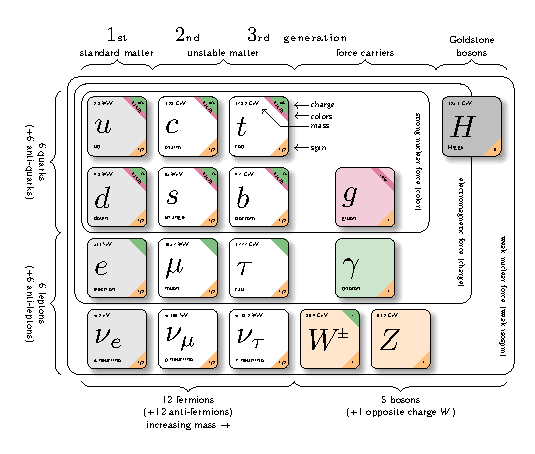
\includegraphics[width=1\linewidth]{fig/chap02-theory/SMpart.pdf}
    \caption{Fundamental particles of the Standard Model \cite{BurgardCarstenStandardExample}}
    \label{fig:SMpart}
\end{figure}

%commented
\iffalse
\paragraph*{Interactions}
The three fundamental interactions described by the SM are the electromagnetic, the strong, and the weak force.\\
Each interaction has a Gauge boson that arises from a symmetry group.\\
The \emph{electromagnetic interaction} is described by the quantum electrodynamics (QED) \cite{FeynmanQED:Matter}, a \U{1} Gauge theory, and is mediated by the photon.\\
The \emph{strong interaction} is described by the quantum chromodynamics (QCD) \cite{Chromodynamics1995QUANTUMCHROMODYNAMICS} through the \SU{3} group.\\

\fi

\paragraph*{Fermions}
Fermions are divided into leptons and quarks, both divided into 3 generations, for a total of 12 fermions.\\
\emph{Quarks} are the constituents of the hadrons. They have a fractional electric charge and a color charge (or an anticolor charge for the antiquarks).\\
Quarks are divided into up-type quarks (up, charm, and top) with an electric charge of $Q=2/3$ and into down-type quarks (down, strange, and bottom) with an electric charge of $Q=-1/3$.
One of the main properties of the QCD is color confinement: isolated particles must be color singlets, so free quarks can't be observed because they hadronize (see sec. \ref{sub:QCD}).
The only exception is the top quark that decays before the hadronization due to its short lifetime.\\
Furthermore, weak interactions don't couple identically with all the flavors: charged weak interactions mix the flavor of the down-type quarks according to the unitary CKM matrix, while neutral weak interactions have different couplings that depend on the weak isospin of the fermion.\\
\emph{Leptons} are the electron (\Pe), the muon (\PGm), the tau (\PGt) and their respective neutrinos (\PGne, \PGnGm, \PGnGt).
A charged lepton and its respective neutrino represent a generation of leptons with a corresponding family lepton flavor number $L_{\ell_i}=n_{\ell_i}-n_{\PAl_i}$ that, in SM, is conserved together with the total lepton number $L=n_\ell-n_\PAl$.
The leptons participate in all the interactions except the strong force.\\


\subsection{Gauge theories and the QED}\label{sub:gauge_qed}
\paragraph*{Fermion free fields}
The Lagrangian (density) for a free fermion field is the Dirac Lagrangian
\begin{equation}\label{eq:Dirac}
\mathcal{L}_{\text{Dirac}}=i\bar{\psi}\gamma^{\mu}\partial_{\mu}\psi-m\bar{\psi}\psi
\end{equation}
where $\aff{\psi}{}=\ff{\psi}{}^\dagger\gamma^0$ is the adjoint Dirac spinor, and $\gamma^\mu$ are the 4 Dirac matrices that obey the Clifford algebra $\{\gamma^\mu,\gamma^\nu\}=2\eta^{\mu\nu}$.\\
The corresponding equation of motion has two solutions: the one with the positive energy represents the fermion field, and the one with the negative energy represents the anti-fermion field.\\
Dirac spinors are representations of the Lorentz group $SO^+(1,3)$ that can be decomposed into the $\SU[L]{2} \otimes \SU[R]{2}$ group.\\
Using this different representation, Dirac spinors can be described in the so-called chiral basis $\psi=\left(\psi_L,\psi_R \right)$ where $\psi_{L/R}$ are called left/right Weyl spinors and are respectively the $\left(\frac{1}{2},0\right)$ and the $\left(0,\frac{1}{2}\right)$ representations of the $\SU{2} \otimes \SU{2}$ group.\\
The chirality operator $\gamma^5=i\gamma^0\gamma^1\gamma^2\gamma^3$ anti-commutes with all the gamma matrices and commutes with the Dirac Hamiltonian only if the mass is zero, so the chirality is a good quantum number only for massless particles.\\
The chirality plays an important role in the weak interaction, as described in sec. \ref{sub:weak}
\paragraph*{Gauge theories}
The standard procedure to introduce a global symmetry in the Lagrangian and a Gauge boson field is the following:
\begin{enumerate}
    \item Introduce a local symmetry based on a Lie group:
    \begin{equation}\label{eq:spinor_gauge}
        \psi(x) \to \psi^\prime (x)=g(x) \psi(x) = e^{i \alpha_a(x) t^a}\psi(x)
    \end{equation}
    where $g(x)$ is a representation of the group and $t^a$ its generators
    \item Replace the partial derivatives $\partial_\mu$ with the covariant derivative $D_\mu$
    \begin{equation}\label{eq:covariant_derivative}
        D_{\mu}\psi(x)=\left(\partial_{\mu}-i g\,A_{\mu}^{a}(x)\,t^{a}\right)\psi(x)\;
    \end{equation}
    where $g$ is the coupling constant between the fermion field and the Gauge fields and $A^a_\mu$ the Gauge fields 
    \item The covariant derivative should transform according to the Gauge group $D_\mu \psi(x)\to g(x) D_\mu \psi(x)$ and, with some calculation, it is possible to find that the Gauge field transform as the following under the action of the Gauge group
    \begin{equation}\label{eq:gauge_field_transformation}
        A_{\mu}(a)\rightarrow g(x)A_{\mu}(x)g^{-1}(x)-\frac i g\,\bigg(\partial_{\mu} g(x)\bigg) g^{-1}(x)\,
    \end{equation}
    where $A_\mu=A_\mu^a(x)t^a$
    \item The final Lagrangian now has a global invariance for the Gauge group and, according to the Noether theorem, there is a conserved charge. Furthermore, in this procedure, another vector massless field arises.
\end{enumerate}
\paragraph*{Quantum electrodynamics}
The simplest case of a Gauge theory is the quantum electrodynamics (QED) \cite{FeynmanQED:Matter} in which the Gauge group is \U{1}, a commutative group for which holds $g(x)g(y)=g(y)g(x)$\\
The fundamental representation of the \U{1} group is $g(x)=e^{i \alpha(x)}$, \ie a local phase.\\
Imposing the \U{1} invariance on the Dirac Lagrangian, we obtain the QED Lagrangian.
\begin{equation}\label{eq:QED}
    \Lg{QED}=i\bar{\psi}\gamma^{\mu}(\partial_{\mu}+i q A_{\mu})\psi-m\bar{\psi}\psi-\frac{1}{4}F^{\mu\nu}F_{\mu\nu}
\end{equation}
where $A_\mu$ is the photon field, $q$ the elementary electron charge and $F_{\mu\nu}=\partial_\mu A_\nu-\partial_\nu A_\mu$ the electromagnetic tensor\\
In the SM, all the fermions, except the neutrinos, have an electric charge and are involved in the electromagnetic interactions.\\


\subsection{Quantum chromodynamics}\label{sub:QCD}
Quantum chromodynamics (QCD) is the \SU{3} Gauge theory that describes the strong interaction and involves gluons and quarks, bonding together into hadronic states.
The quantum number related to strong interaction is the color charge.
Applying the gauging technique described in the section \ref{sub:gauge_qed} is possible to obtain the QCD Lagrangian.
\begin{equation}\label{eq:QCD}
    \Lg{QCD}=-i g_{s}\bar{\psi}\gamma^{\mu}\lambda_{a}\psi G_{\mu}^a-\frac{1}{4}G_{a}^{\mu\nu}G_{\mu\nu}^a
\end{equation}
where \(G_{\mu\nu}^{a}=\partial_{\mu}G_{\nu}^{a}-\partial_{\nu}G_{\mu}^{a}-g_{s}f^{a b c}G_{\mu}^{b}G_{\nu}^{c}\) is the corresponding of the electromagnetic tensor for the strong force, $\lambda_a$ are the \SU{3} generators, and $f^{abc}$ the \SU{3} structure constants.\\
Each quark carries a color charge and each anti-quark an anticolor charge and, since \SU{3} has 8 generators, 8 gluons exist (or just one gluon that can carry one of 8 possible couples of color-anticolor).\\
There are significant differences with the QED due to the non-abelianity of \SU{3}:
\begin{itemize}
    \item \textbf{Gluon self-coupling}: gluons can interact with each other.
    \item \textbf{Asymptotic freedom}: the coupling strength decreases with the energy, \ie at large energy scales the quarks become quasi-free.\\
    The coupling constant of the strong interaction depends on the energy scale \cite{Deur2016TheCoupling}
    \begin{equation}\label{eq:alphas_run}
        \alpha_S(\mu^2)\propto \frac{1}{\ln \left( \frac{\mu^2}{\Lambda_{\text{QCD}}^2}\right)}        
    \end{equation}
    Where $\Lambda_{QCD}\approx 200 \MeV$ and $\mu$ is the energy scale.\\
    When $\mu \gg \Lambda_{QCD}$, strong interactions can be described using perturbative techniques (pQCD) but, at low-energy scales, the QCD is non-perturbative and that leads to the third property of the QCD
    \item \textbf{Color confinement}: At low-energy scales, the strong coupling is so large that quarks are always bounded in color singlets and isolated quarks can't be observed.\\
    This is also why the strong force is a short-range interaction, while the electromagnetic force is a long-range interaction.
\end{itemize}

\subsection{Electroweak unification}\label{sub:weak}
\paragraph*{Weak interactions}
The weak interaction was first introduced by Enrico Fermi to explain the $\beta$ decay through the 4-point Fermi interaction \cite{Fermi1934Tentativo} and is the only force that involves all the fermions and that violates the parity and the charge parity conservation. \\
The quantum number related to the weak interaction is the weak isospin, generated by the \SU{2} gauge group that creates 3 gauge bosons: the $W^\pm$ and the $Z$ bosons.\\
Trying to build the weak Lagrangian only using the gauging technique described in the section \ref{sub:gauge_qed} doesn't work in this case for different reasons:
\begin{itemize}
    \item The W boson and the Z boson would have the same coupling to the fermions, while experimentally this was disproven. To address this problem, the weak interaction was unified with the electromagnetic interaction.
    \item The W/Z bosons are proven to be massive bosons, while gauge bosons are always massless. The massive term can't be added arbitrarily to the Lagrangian because such a theory would be non-renormalizable, so they have to be added through the Higgs mechanism as described in the section \ref{sub:SM}.\\
    The non-zero W/Z mass  is also the cause of why the weak interactions have a finite range, given that the weak interactions are suppressed by the weak propagator $1/(q^2-M_{W/Z}^2)$.
    \item The weak interaction doesn't couple identically with all the quarks, but the down-type flavors are mixed by the Cabibbo-Kobayashi-Maskawa (CKM) matrix \cite{Kobayashi1973CP-ViolationInteraction}, as described in section \ref{sec:CKM}. The elements of the CKM matrix are complex, and this leads to the CP violation.
    \item To introduce the parity violation in the Lagrangian, the $\gamma^\mu$ in the interaction term of the Lagrangian has to be replaced with $\gamma^\mu \left(1-\gamma^5 \right)/2 $.\\
    The term $(1-\gamma^5)/2$ is the left chirality projector, and this implies that weak interaction couples only with the left part of the spinor. This will turn out to be true only for charged weak interactions, while for neutral weak interactions, the mixing between the photon and the Z boson in the electroweak (EW) unification process will reintroduce the coupling with the right spinors.
\end{itemize}

\paragraph*{Electroweak unification}\label{sub:EW}
The electromagnetic and weak interactions were unified in the Glashow-Weinberg-Salam theory \cite{Weinberg1967ALeptons,Salam1964ElectromagneticInteractions,Glashow1961PartialInteractions} based on the $\SU{2} \otimes \U(1)$ symmetry group.\\
We start defining left-handed doublets and right-handed singlets
\begin{align}
    Q_{L,i}=\left({u_{L,i}}\atop{d_{L,i}}\right), \quad u_{R,i},\quad d_{R,i} \\
    \mathcal{L}_{L,i}=\left(\begin{array}{l}{{\nu_{L,i}}}\\ {{\ell_{L,i}}}\end{array}\right),\quad\ell_{R,i}
\end{align}
so left-handed particles organize in $\SU{2}$ doubles while right-handed particles in $\SU{2}$ singlets.
The gauge invariant Lagrangian for the group $\SU{2}\otimes\U{1}$ is:
\begin{equation}\label{eq:EWK_preunification}
{\mathcal{L}}=i\overline{{{L}}}\gamma^{\mu}D_{\mu}L+\overline{{{R}}}i\gamma^{\mu}D_{\mu}R-\frac{1}{4}B^{\mu\nu}B_{\mu\nu}-\frac{1}{4}W_{a}^{\mu\nu}W_{\mu\nu}^{a}
\end{equation}
where
\begin{itemize}
    \item L and R are the left doublets and the right singlets
    \item $D_{\mu}=\partial_{\mu}-i{\frac{g^{\prime}}{2}}\hat{Y}B_{\mu}-i g\hat{T}_{i}W_{\mu}^{i}$ is the covariant derivative
    \item $\hat{Y}$ is the \U{1} generator (the hypercharge operator)
    \item $\hat{T}_i$ are the three \SU{2} generators (weak isospin operators)
    \item $B^{\mu\nu}=\partial_{\mu}B_{\nu}-\partial_{\nu}B_{\mu}$, where $B_\mu$ is the \U{1} gauge field
    \item $W_{\mu\nu}^{i}=\partial_{\mu}W_{\nu}^{i}-\partial_{\nu}W_{\mu}^{i}-g\epsilon^{i j k}W_{\mu}^{j}W_{\nu}^{k}$ where $W^i_\mu$ are the 3 \SU{2} gauge fields and $\epsilon^{ijk}$ the \SU{2} structure constants. 
\end{itemize}
The experimental observed W, Z and $\gamma$ bosons can be expressed as a linear combination of the defined gauge fields.
\begin{gather}
    W_\mu^{\pm}=(W^1_\mu\pm i W^2_\mu)/\sqrt{2}\\
    \db{A_\mu}{Z_\mu}=\left(\begin{array}{l l}{{\cos\theta_{W}}}&{{\sin\theta_{W}}}\\ {{-\sin\theta_{W}}}&{{\cos\theta_{W}}}\end{array}\right)\db{B_\mu}{W^3_\mu}
\end{gather}
where the mixing angle $\theta_W$ is the Weinberg angle, and it can be proven that $\cos(\theta_W)=m_W/m_Z$.\\
After the mixing, we can break the electroweak Lagrangian into different pieces:
\begin{equation}\label{eq:EWK}
    \Lg{EWK}=\Lg{kin}+\Lg{QED}+\Lg{wcc}+\Lg{wnc}+\Lg{gauge}
\end{equation}

\begin{itemize}
    \item  $\Lg{kin}$ is the fermions kinetic term
    \item $\Lg{QED}$ is the interaction term of the QED Lagrangian described in section \ref{sub:gauge_qed}
    \item $\Lg{wcc}$ is the interaction term of the weak-charged currents
    \begin{equation}
        {\mathcal{L}}_{wcc}\,=\,\frac{g}{2{\sqrt{2}}}\,\left\{W_{\mu}^{\dagger}\,\bar{L}\gamma^{\mu}(1-\gamma_{5})L+\,\dots \right\}
    \end{equation}
    the charged weak interactions preserve the vector minus axial (V-A) structure, and this implies that the $W^\pm$ bosons interact only with the left doublets.\\
    Furthermore, the weak interactions mix the down-type quark flavors so the terms that involve quarks have to include a unitary matrix, the CKM matrix. (see sec.\ref{sec:CKM})
    \begin{equation}
        \Lg{wcc}^q=-\frac{g}{\sqrt{2}}(\overline{{{u}}}_{L},\overline{{{c}}}_{L},\overline{{{t}}}_{L})\gamma^{\mu}W_{\mu}^{+}V_{\mathrm{CKM}}\tb{d_{L}}{s_{L}}{b_L}+\dots
    \end{equation}
    This also does not allow the presence of flavour-changing neutral currents (FCNC).
    \item $\Lg{wnc}$ is the interaction term of the weak neutral currents,
    \begin{equation}
        \Lg{wnc}=\frac{e}{2\sin\theta_{W}\cos\theta_{W}}\,Z_{\mu}\sum_{f}\,\bar{f}\gamma^{\mu}(v_{f}-I^3_{f}\gamma_{5})\,f\;
    \end{equation}
    where $I^3_f$ is the weak isospin of the fermion and $v_f=I^{3}_{f}\left(1-4|Q_{f}|\sin^{2}\theta_{W}\right)$.
    Unlike the W boson, the Z boson interacts both with the left and the right part of the spinor with different couplings depending on the isospin and the charge of the fermion 
    \item $\Lg{gauge}$ is the kinematic part of the Lagrangian related to the Gauge bosons
\end{itemize}


\subsection{The spontaneous symmetry breaking}\label{sub:SM}
The EW Lagrangian in \Eq{eq:EWK} does not include both the fermions and the boson masses.
In the SM, the W/Z masses are generated by the Higgs-Brout-Englert mechanism \cite{Higgs1964BrokenBosons,Englert1964BrokenMesons}.
Starting from the  $\SU[C]{3} \otimes \SU[L]{2} \otimes \U[Y]{1}$ Lagrangian,
\begin{equation}
    \Lg{}=\Lg{kin}+\Lg{QCD}+\Lg{EWK}
\end{equation}
we add another term introducing a scalar complex doublet field
\begin{equation}\label{eq:Higgs_preSSB}
    \Lg{H}=(D^{\mu}\phi)^{\dagger}(D_{\mu}\phi)-\frac{1}{2}\mu^{2}(\phi^{\dagger}\phi)-\frac{1}{4}\lambda(\phi^{\dagger}\phi)^{2}
\end{equation}
where $D_\mu$ is the electroweak covariant derivative defined in \Eq{eq:EWK_preunification} and $\mu^2<0$.
The last 2 terms form the Higgs potential $V(\phi)$, represented in \Fig{fig:HiggsPotential}.

The minimum of $V(\phi)$ is not unique, and the choice of a specific minimum for $\phi$ leads to the spontaneous symmetry breaking (SSB) of the $\SU{3} \otimes \SU{2} \otimes \U{1}$ group into the $\SU{3} \otimes \U{1}$ group.\\
A convenient choice is to pick the ground state of $\phi$ as
\begin{equation}
    \langle\phi\rangle=\frac{1}{\sqrt{2}}\db{0}{v}=\frac{1}{\sqrt{2}}\db{0}{\sqrt{\frac{-\mu^2}{\lambda}}}
\end{equation}
Developing the Lagrangian in \Eq{eq:Higgs_preSSB} around this minimum, we can redefine the scalar doublet as
\begin{equation}\label{eq:higgs_intro}
    \phi=\frac{1}{\sqrt{2}}\db{0}{v+H(x)}
\end{equation}
and the potential $V(\phi)$ expanded in powers of the new real Higgs field $H(x)$ becomes
\begin{equation}
    V(H)=-\frac{1}{2}\mu^{2}H^{2}-\frac{\mu^{2}}{2\nu}H^{3}-\frac{\mu^{2}}{8\nu^{2}}H^{4}
\end{equation}
Replacing \Eq{eq:higgs_intro} into the \Eq{eq:Higgs_preSSB} the W/Z bosons acquire a mass term with
\begin{gather}
    M_{W^\pm}=\frac{1}{2}gv\\
    M_Z=\frac{M_{W^\pm}}{\cos (\theta_W)}
\end{gather}
This also generates the Higgs boson mass $m_H=\sqrt{2\lambda}\mu$, the interactions between the Higgs boson and the vector bosons, and the Higgs self-interactions.
\begin{figure}[h!]
    \centering
    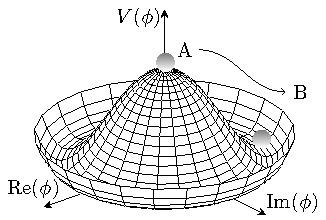
\includegraphics[width=0.7\linewidth]{fig/chap02-theory/higgs.pdf}
    \caption{Illustration of the Higgs potential $V(\phi)$ \cite{HiggsTikZ.net}}
    \label{fig:HiggsPotential}
\end{figure}\\
\paragraph*{Fermion masses}
The Lagrangian $\Lg{}=\Lg{kin}+\Lg{QCD}+\Lg{EWK}+\Lg{H}$ does not contain the fermion masses yet.\\
The mass terms of the Dirac Lagrangian (\Eq{eq:Dirac}) can't be added directly because the term \(-m \bar{\psi} \psi\) is not invariant under $\SU{2}\otimes \U{1}$.
This problem can be addressed by introducing the Yukawa interaction between fermions and the Higgs field
\begin{equation}
    \Lg{Yukawa}=-\left(g_{i j}^{d}\bar{Q}_{L,i}\phi d_{R,j}+g_{i j}^{u}\bar{Q}_{L,i}(i\sigma^{2}\phi^{\dagger})u_{R,j}+g_{i j}^{\ell}\bar{\mathcal{L}}_{L,i}\phi\ell_{R,j}\right)+h.c.
\end{equation}
After the SSB, the masses of the fermions arise from the Yukawa interaction.
\begin{gather}
    \Lg{masses}=-M_{i j}^{\ell}\bar{\ell}_{L,i}\ell_{R,j}-M_{i j}^{d}\bar{d}_{L,i}d_{R,j}-M_{i j}^{u}\bar{u}_{L,i}u_{R,j}\\
    M^{\ell,d,u}=\frac{v}{\sqrt{2}}g^{\ell,d,u}
\end{gather}
The non-diagonal quark mass matrix $M$ can be diagonalized through a unitary transformation, which is equivalent to a basis change.
\begin{equation}
    M_{\text{diag}}^{u/d}=(V_L^{u/d})^\dagger M^{u/d} V_R^{u/d}
\end{equation}
This transformation is the one that induces the mixing of mass eigenstates between the left-handed fermion and the \PW boson field.
Indeed, the flavor mixing represented by the CKM matrix can be expressed in terms of these unitary transformations.
\begin{equation}
    V_{CKM}=(V_L^u)^\dagger V_L^d
\end{equation}
At this point, the SM is complete. A summary of all the particles of the SM and their quantum numbers is shown in Tab. \ref{tab:SM}
\\
\\
%!TEX root = ../thesis.tex

% TABLE: SM Summary
%   https://en.wikipedia.org/wiki/File:Electroweak.svg
%   https://commons.wikimedia.org/wiki/File:Standard_Model.svg
%   https://en.wikipedia.org/wiki/Mathematical_formulation_of_the_Standard_Model#Field_content_in_detail
\begin{table}[h!]
\vspace*{-6mm}
\centering
\caption{
Summary of the representation and quantum numbers SM fields.
Bold numbers indicate the dimension of the representation under the respective gauge group.
}\label{tab:SM_symmetries}
\def\arraystretch{1.3}
\def\vsdb{\rule[-15pt]{0pt}{36pt}} % vertical space for doublet
\begin{tabular}{llc@{\extracolsep{\tabcolsep}}c@{\extracolsep{4pt}}c@{\extracolsep{\tabcolsep}}c@{\extracolsep{1.5\tabcolsep}}c}
  \hline
  %Field name  & Symbol      & $\SU[C]{3}$ & $\SU[L]{2}$ & $T_3$ & $\YW/2$ & $Q = T_3 + \YW/2$ \\
  \multirow{2}{*}{Field name}
        & \multirow{2}{*}{Symbol}
               & \multicolumn{2}{c}{Representations} & \multicolumn{3}{c}{Quantum numbers} \\
                 \cline{3-4}                           \cline{5-7}
        &      & $\SU[C]{3}$ & $\SU[L]{2}$ & $T_3$ & $\YW/2$ & $Q = T_3 + \YW/2$ \\
  \hline
  \vsdb % add vertical space above & below
  Quark doublet
        & $\ff{Q}{L} = \db{\ff{u}{L}}{[1pt]\ff{d}{L}}$
               & \textbf{3}  & \textbf{2} & $\db{+\frac{1}{2}}{[2pt]-\frac{1}{2}}$
                                                   & $+\frac{1}{6}$
                                                             & $\db{+\frac{2}{3}}{[2pt]-\frac{1}{3}}$ \\[2mm]
  Up-quark singlet
        & $\ff{u}{R}$  & \textbf{3}  & \textbf{1} & $+\frac{2}{3}$
                                                   & $+\frac{2}{3}$
                                                             & $+\frac{2}{3}$ \\
  Down-quark singlet
        & $\ff{d}{R}$  & \textbf{3}  & \textbf{1} & $-\frac{1}{3}$
                                                   & $-\frac{1}{3}$
                                                             & $-\frac{2}{3}$ \\
  \vsdb % add vertical space above & below
  Lepton doublet
        & $\ff{L}{L} = \db{\ff{\nu}{L}}{[1pt]\ff{e}{L}}$ 
                       & \textbf{1}  & \textbf{2} & $\db{+\frac{1}{2}}{[2pt]-\frac{1}{2}}$
                                                   & $-\frac{1}{2}$
                                                             & $\db{\phmin0}{-1}$ \\[2mm]
  Lepton singlet
        & $\ff{e}{R}$  & \textbf{1}  & \textbf{1} & $\phmin0$
                                                   & $-1$    & $-1$ \\
  \hline
  Gluon field
        & $G^a_\mu$    & \textbf{8}  & \textbf{1} & $\phmin0$
                                                   & $\phmin0$ & $\phmin0$ \\
  \rule[-19pt]{0pt}{42pt}% % add vertical space above & below
  Weak gauge field
        & $W^i_\mu = \db{W^+_\mu}{W^-_\mu\\W^3_\mu}$
                       & \textbf{1}  & \textbf{3} & $\db{+1}{-1\\\phmin0}$
                                                   & $\phmin0$ & $\db{+1}{-1\\\phmin0}$\\
  Hypercharge field
        & $B_\mu$
                       & \textbf{1}  & \textbf{1} & $\phmin0$
                                                   & $\phmin0$ & $\phmin0$ \\
%  Weak gauge bosons
%        & $\db{W^+_\mu}{W^-_\mu\\Z^0_\mu}$
%               & \textbf{1}  & \textbf{3} & $\db{+1}{-1\\0}$
%                                                   & \phmin0 & $\db{+1}{-1\\\phmin0}$\\
%  Photon
%        & $A^a_\mu$    & \textbf{1}  & \textbf{1} & $\phmin0$
%                                                   & $\phmin0$ & $\phmin0$ \\
  \hline
  \vsdb % add vertical space above & below
  Higgs doublet
        & $\Phi = \db{\phi^+}{[1pt]\phi^0}$
               & \textbf{1}  & \textbf{2} & $\db{+\frac{1}{2}}{[2pt]-\frac{1}{2}}$
                                                   & $+\frac{1}{2}$
                                                             & $\db{+1}{\phmin0}$ \\[2mm]
  \vsdb % add vertical space above & below
  Conjugate Higgs doublet
        & $\Phi^\mathrm{c} = \db{\phi^{0*}}{[1pt]\phi^-}$
               & \textbf{1}  & \textbf{2} & $\db{+\frac{1}{2}}{[2pt]-\frac{1}{2}}$
                                                   & $-\frac{1}{2}$
                                                             & $\db{\phmin0}{-1}$ \\[2mm]
  \hline
\end{tabular}
\label{tab:SM}
\end{table}








\section{The CKM matrix}\label{sec:CKM}
As already discussed, the weak interactions mix the down-type quarks with the Cabibbo-Kobayashi-Maskawa (CKM) matrix \cite{Cabibbo_angle,Kobayashi1973CP-ViolationInteraction}.
\begin{equation}
    \Lg{wcc}^q=-\frac{g}{\sqrt{2}}(\overline{{{u}}}_{L},\overline{{{c}}}_{L},\overline{{{t}}}_{L})\gamma^{\mu}W_{\mu}^{+}V_{\mathrm{CKM}}\tb{d_{L}}{s_{L}}{b_L}+\dots
\end{equation}
\begin{equation}
V_{C K M}=\left(\begin{array}{l l l}{{V_{u d}}}&{{V_{u s}}}&{{V_{u b}}}\\ {{V_{c d}}}&{{V_{c s}}}&{{V_{c b}}}\\ {{V_{t d}}}&{{V_{t s}}}&{{V_{t b}}}\end{array}\right)\,
\end{equation}
The CKM matrix is a $3 \times 3$ complex matrix that can be written in terms of 18 real parameters. The unitarity condition $V^\dagger V= 1\kern-0.25em\text{l}$ adds 9 constraints, and the 6 quark fields can absorb the phases defining a new common phase, so the number of parameters of the CKM matrix is four.\\
These parameters can be determined through global fits that combine experimental data from different experiments, imposing the constraints of the standard model (\eg the unitarity), or can be measured independently \cite{PDG_2022}.\\
Measure all the parameters independently allows us to verify the unitarity of the CKM matrix that, if violated, can be a sign of new physics.\\
The $|V_{ud}|$ is the element measured with the highest precision through  the study of $\beta$ decays. The other $|V_{uq}|$ and $|V_{cq}|$ elements are measured through leptonic and semileptonic meson decays, but these kinds of measures are highly affected by theoretical uncertainties due to the non-perturbative nature of the strong interaction at low energy that bonds the quarks in the meson.
The $|V_{tq}|$ elements are not affected by non-perturbative QCD uncertainties, but the QCD background of a hadron collider makes their measure challenging and, at this time, an electron-positron collider with sufficient energy in the center of mass to produce a top quark does not exist yet.
\\
\\
There are two common parametrizations of the CKM matrix: the standard parametrization and the Wolfenstein parametrization \cite{PDG_2022}.
The values of the parameters listed below are the ones obtained by the CKMfitter group through a global fit \cite{Charles2005CPFactories,Hocker2001AMatrix,PDG_2022}.
\paragraph*{Standard parametrization}
In the standard parametrization, the CKM matrix is expressed as the product of 3 rotation matrices with the addition of a phase.
\begin{equation}
    V_{C K M}=\left(\begin{array}{c c c c}{{1}}&{{0}}&{{0}}\\ {{0}}&{{c_{23}}}&{{s_{23}}}\\ {{0}}&{{-s_{23}}}&{{c_{23}}}\end{array}\right)\left(\begin{array}{c c c}{{c_{13}}}&{{0}}&{{s_{13}e^{-i\delta}}}\\ {{0}}&{{1}}&{{0}}\\ {{-s_{13}e^{i\delta}}}&{{0}}&{{c_{13}}}\end{array}\right)\left(\begin{array}{c c c}{{c_{12}}}&{{s_{12}}}&{{0}}\\ {{-s_{12}}}&{{c_{12}}}&{{0}}\\{{0}}&{0}&{1}\end{array}\right)
\end{equation}
where  $c_{ij}=\cos{\theta_{ij}}$, $s_{ij}=\sin(\theta_{ij})$ and $\delta$ is the phase responsible for the CP violation in weak interactions.\\
The values obtained by the CKMfitter group are the following
\begin{equation}
    \begin{array}{l l}{{\sin\theta_{12}=0.22500\pm0.00085\,,~~~~~}}&{{\sin\theta_{13}=0.00369\pm0.00011\,,}}\\ {{\sin\theta_{23}=0.04182_{-0.00074}^{+0.00067\,,}~~~~}}&{{\delta=1.144\pm0.027\,.}}\end{array}
\end{equation}


\paragraph*{Wolfenstein's parametrization}
Defining new four real parameters, 
\begin{gather}
    s_{12}=\lambda={\frac{|V_{u s}|}{\sqrt{|V_{u d}|^{2}+|V_{u s}|^{2}}}} ,\\
    s_{23}=A\lambda^{2}=\lambda|\frac{V_{c b}}{V_{u s}}|,\\
    s_{13}e^{i\delta}=A\lambda^{3}(\rho+i\eta)=\frac{A\lambda^{3}(\bar{\rho}+i\bar{\eta})\sqrt{1-A^{2}\lambda^{4}}}{\sqrt{1-\lambda^{2}}\left[1-A^{2}\lambda^{4}(\bar{\rho}+i\bar{\eta})\right]}\,
.
\end{gather}
the Wolfenstein parameterization shows clearly the order of magnitude of the different elements in powers of $\lambda$
\begin{equation}
    V_{C K M}\simeq\left(\begin{array}{c c c}{{1-\frac{\lambda^{2}}2\ \ \ }}&{{\lambda}}&{{\lambda^{3}(\rho-i\eta)}}\\ {{-\lambda}}&{{1-\frac{\lambda^{2}}2\ \ \ }}&{{A\lambda^{2}}}\\ {{A\lambda^{3}(1-\rho-i\eta)}}&{{-A\lambda^{2}}}&{{1}}\end{array}\right)+{\cal O}(\lambda^{4}).
\end{equation}
The CKMfitter group performed a global fit for this parametrization as well.
\begin{equation}
    \begin{array}{l l}{{\lambda=0.22500\pm0.00067\,,~~~~}}&{{A=0.826_{-0.015}^{+0.018}\,,}}\\ {{\bar{\rho}=0.159\pm0.010\,{,~~~}}}&{{\bar{\eta}=0.348\pm0.010\,.}}\end{array}
\end{equation}
and the fit result of the magnitudes of the CKM elements is:
\begin{equation}
|V_{\mathrm{CKM}}|=\left(\begin{array}{l l l}{{0.97435\pm0.00016}}&{{0.22500\pm0.00067}} & {{0.00396\pm0.00011}}\\ {{0.22486\pm0.00067}}&{{0.97349\pm0.00016}}&{{0.04182^{+0.00085}_{-0.00074}}}\\ {{0.00857_{-0.00018}^{+0.00020}}}&{{0.04110_{-0.00072}^{+0.00083}}}&{{0.999118^{+0.000031}_{-0.000036}}}\end{array}\right).
\end{equation}
\paragraph*{Unitarity triangle}
The unitarity constraints of the CKM matrix are:
\begin{gather}
    \sum_i V_{ij}V_{ik}^*=\delta_{jk} \quad ; \quad 
    \sum_j V_{ij}V_{kj}^*=\delta_{ik}
\end{gather}
These constraints can be represented in the complex $(\bar{\rho},\bar{\eta})$ plane in a triangle with vertexes $(0,0), (1,0), (\bar{\rho},\bar{\eta})$ (\Fig{fig:triangle}). The area of the unitarity triangle is also a measure of the CP violation of the weak interactions.
\begin{figure}[h!]
    \centering
    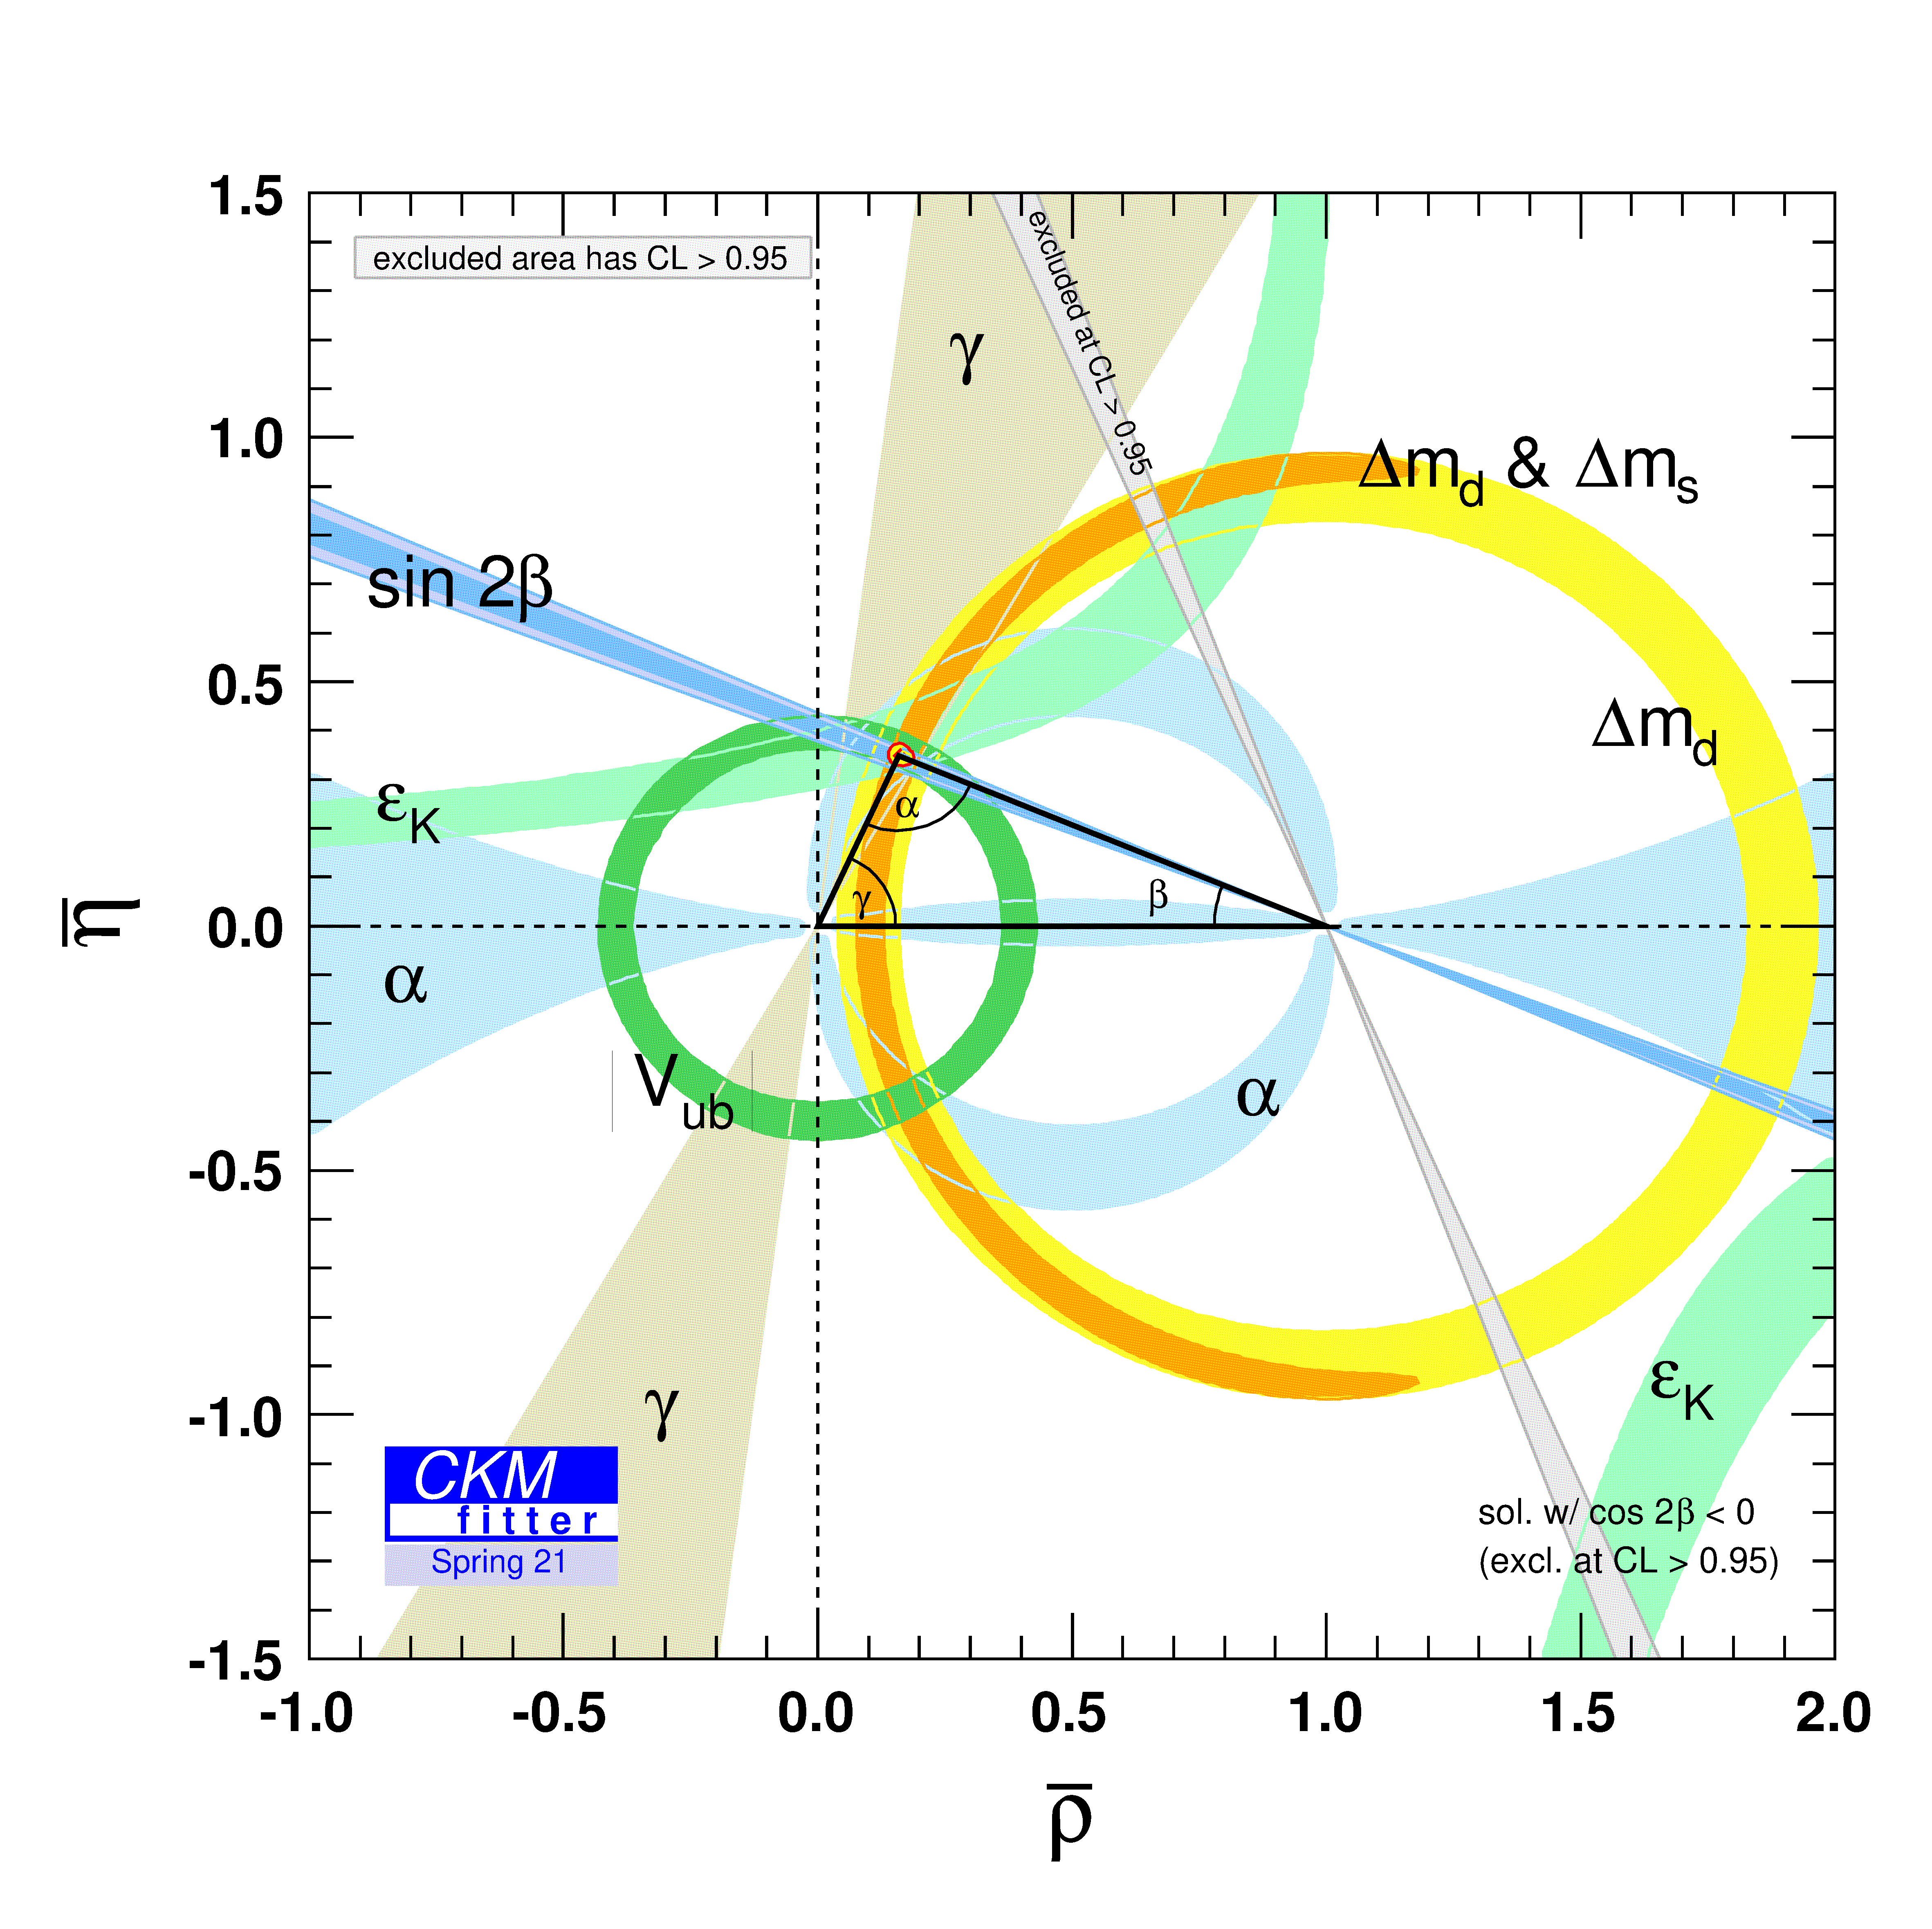
\includegraphics[width=0.69\linewidth]{fig//chap02-theory/triangle.png}
    \caption{CKMfitter global constraints on the unitarity triangle \cite{CKMfitter}. Shaded areas correspond to 95\% CL}
    \label{fig:triangle}
\end{figure}




\newchap{The $|V_{cb}|$ CKM element}\label{sec:vcb}
\vspace{-1cm}
\minitoc
\section{The $V_{cb}$ element}\label{sec:vcb}
\begin{minipage}{\linewidth}
    \begin{minipage}{0.43\linewidth}
        The $V_{cb}$ element plays an important role in the unitarity of the CKM matrix. The radius of the unitarity-clock, the green circle centered in the origin in \Fig{fig:triangle}, is proportional to the ratio $|V_{ub}/V_{cb}|$, so $V_{cb}$ normalize the whole triangle \cite{Ricciardi2019DeterminationV_cb}.\\
        \\
        $|V_{cb}|$ is measured from the semileptonic inclusive and exclusive $b \to c\ell\nu$
        decays but the parton level amplitude, that is proportional to $|V_{cb}|^2$, has to be corrected by introducing form factors that take into account the contributions by strong interactions in the meson. These corrections inevitably lead to theoretical uncertainties that are of the same order as the experimental systematic uncertainties.
    \end{minipage}
    \hfill
    \begin{minipage}{0.55\linewidth}
        \vspace{-1.25cm}
        \begin{figure}[H]
            \centering
            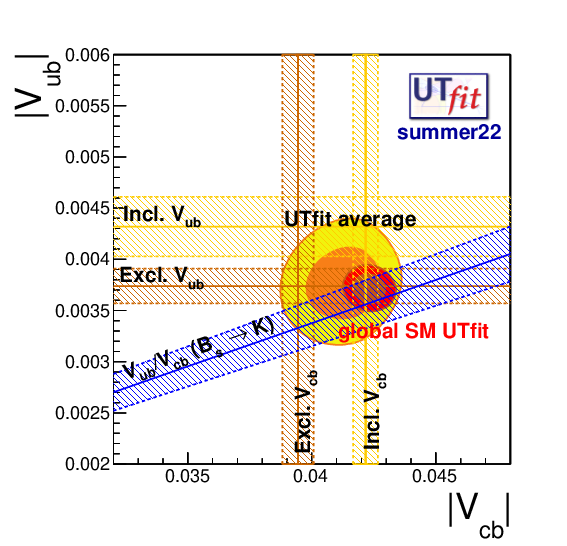
\includegraphics[width=\linewidth]{fig//chap02-theory/vubvcb.png}
            \caption{$|V_{cb}|$ and $|V_{ub}|$ global fit and averages of inclusive and exclusive measurements performed by the UTfit collaboration \cite{Bona2023NewScheme}}
            \label{fig:vcbvub}
        \end{figure}
    \end{minipage}
\end{minipage}
\\
\\
Furthermore, the inclusive and exclusive measurements of the $V_{cb}$ element have always been incompatible and separated by $\sim 2 \sigma$ as shown in \Fig{fig:vcbvub}.\\
Recently, a revision of the techniques involved in the calculations of the QCD contributions has narrowed the gap, but the $V_{cb}$ puzzle is still unresolved \cite{Bona2023NewScheme}.\\
These issues also concern the $|V_{ub}|$ measurements.\\
\\
A summary of the single measurements of the $|V_{cb}|$ element can be found in \cite{PDG_2022}.
\subsection{$|V_{cb}|$ from semileptonic B meson decays}
\paragraph*{Inclusive measurement}
The inclusive channel $B\to X_c \ell \nu$ is less model dependent than the exclusive one \cite{Smith2005DeterminationSpectra}.
The QCD contributions can be included by adding two terms in the amplitude: a perturbative term and a non-perturbative term.
\begin{equation}
    \Gamma(B\rightarrow X_c\ell\nu)=\frac{G_{F}^{2}m_{b}^{5}|V_{c b}|^{2}}{192\pi^{3}}[1+P(\alpha_{s},\mu,m_{b}/m_{c})+N(m_b,m_c,\mu_\pi^2,\mu_G^2,\rho_D^2,\rho_{LS}^3)]
\end{equation}
The QCD corrections are computed using the so-called Operator Product Expansion (OPE). OPE allows us to express the widths and moments of the kinematic distributions as a double expansion in $\alpha_S$ and $\Lambda_{QCD}/m_b$. These corrections are actually known up to the third order in $\Lambda_{QCD}/m_b$ \cite{Alberti2016TheVcb}.\\
This expansion depends on other parameters defined in the framework of the heavy quark effective field theory (HQET) that can be constrained through the study of other observables like the lepton energy, the transferred momentum or the hadronic mass \cite{Smith2005DeterminationSpectra} so the final fit has to be performed on an order of $\mathcal{O}(100)$ of observables.\\
The uncertainties of the inclusive measurements of $|V_{cb}|$ are  $\simeq 2\%$, mainly driven by theoretical uncertainties related to the determination of the HQET parameters \cite{Alberti2016TheVcb}.\\
The average of the inclusive measurements is \cite{Bordone2021ThreeVcb}
\begin{equation}
    |V_{cb}|\times10^3\text{ (incl)}=42.16\pm 0.50
\end{equation}

\paragraph*{Exclusive measurement}
The two main exclusive channels studied for $|V_{cb}|$ determination are the $\PAB \to D^* \ell \PAGnl$ and the $\PAB \to D \ell \PAGnl$.
The first channel was measured with an uncertainty of $\simeq 2\%$ with comparable contributions from theory and experiment, while the latter was measured with an uncertainty of the $\simeq 3\%$ but recently
some questions about the form factor parametrization were raised.\\
The exclusive measurement requires knowing six form factors that can be computed using lattice QCD (LQCD) techniques. In the limit of heavy quarks, the six form factors collapse into a single one, and corrections to the $m_b \to \infty$ limit can be obtained through the HQET framework \cite{PDG_2022}.\\
The average of the exclusive measurements is \cite{Bona2023NewScheme}
\begin{equation}
    |V_{cb}|\times10^3\text{ (excl)}=39.44\pm 0.63
\end{equation}

\section{CKM measurements from hadronic W decays}
\subsection{LEP2 measurements}
The Large Electron-positron Collider (LEP) was an electron-positron collider that reached a peak energy in the center of mass of 209 GeV. It was built at CERN and is located in the tunnel that now hosts the LHC accelerator facility and started its physics program in 1989.\\
\\
The LEP2 physics program started in 1996, running at a center of mass energy  that was increased from the Z resonance to 202\GeV at the end of 1999, above the production threshold of WW pairs. 
In this period, the four LEP experiments, ALEPH, DELPHI, L3, and OPAL have collected  $\sim450 \text{pb}^{-1}$ of data above the WW pair production threshold, corresponding to over 6000 WW events per experiment \cite{Nowell2000MeasurementLEP2}.\\
With more than 8000 hadronic W decays, the LEP experiments were able to access some CKM elements directly from W decays.

\paragraph*{Rate of charm production}
ALEPH and OPAL performed a measure of the rate or $W\to cX$ decays on both semileptonic and fully hadronic WW pairs.
\begin{equation}
    R_c^W=\frac{\Gamma(W\to cX)}{\Gamma(W\to q\bar{q})}=\frac{|V_{cd}|^2+|V_{cs}|^2+|V_{cb}|^2}{|V_{cd}|^2+|V_{cs}|^2+|V_{cb}|^2+|V_{ud}|^2+|V_{us}|^2+|V_{ub}|^2}
\end{equation}
This is a unitarity test of the second row of the CKM matrix, indeed, if the unitarity hypothesis holds, it has to be $R_c^W=0.5$.
\\
\\
ALEPH performed the measurement extracting $R_c^W$ with a binned maximum-likelihood fit on the shape of the most c tagged jet.\\
The charm jet tagger was a feed-forward neural network with 12 variables as input that uses mainly information from charm lifetime, jet-shape properties, reconstruction of D mesons, and lepton identification.\cite{Barate1999ATag} \\
\\
On the other hand, OPAL used a relative likelihood discriminant calculated for each jet to separate jets originating from
charm quarks and jets from light quarks. This discriminant relies on jet and event shape properties,
lifetime information, and lepton identification \cite{Abbiendi2000ADecays}.
\\
\\
The results of both experiments are consistent with the unitarity hypothesis with an uncertainty of $\sim 10\%$
\begin{equation}
\begin{aligned}
    R_c^W&=0.51 \pm 0.05 \text{ (stat)} \pm 0.03 \text{ (syst)} & \text{(ALEPH)}\\
    R_c^W&=0.481 \pm 0.042 \text{ (stat)} \pm 0.032 \text{ (syst)} & \text{(OPAL)}
\end{aligned}
\end{equation}
$R_C^W$ allow also an indirect measure of $|V_{cs}|$, subtracting the other $|V_{cx}|$ CKM elements in quadrature from $R_C^W$ obtained from other determinations.

\begin{equation}
\begin{aligned}
    |V_{cs}|&=1.00\pm0.11  \text{ (stat)} \pm 0.07 \text{ (syst)} & \text{(ALEPH)}\\
    |V_{cs}|&=0.969\pm0.058 & \text{(OPAL)}
\end{aligned}
\end{equation}
\begin{figure}[H]
    \begin{subfigure}{0.49\linewidth}
        \centering
         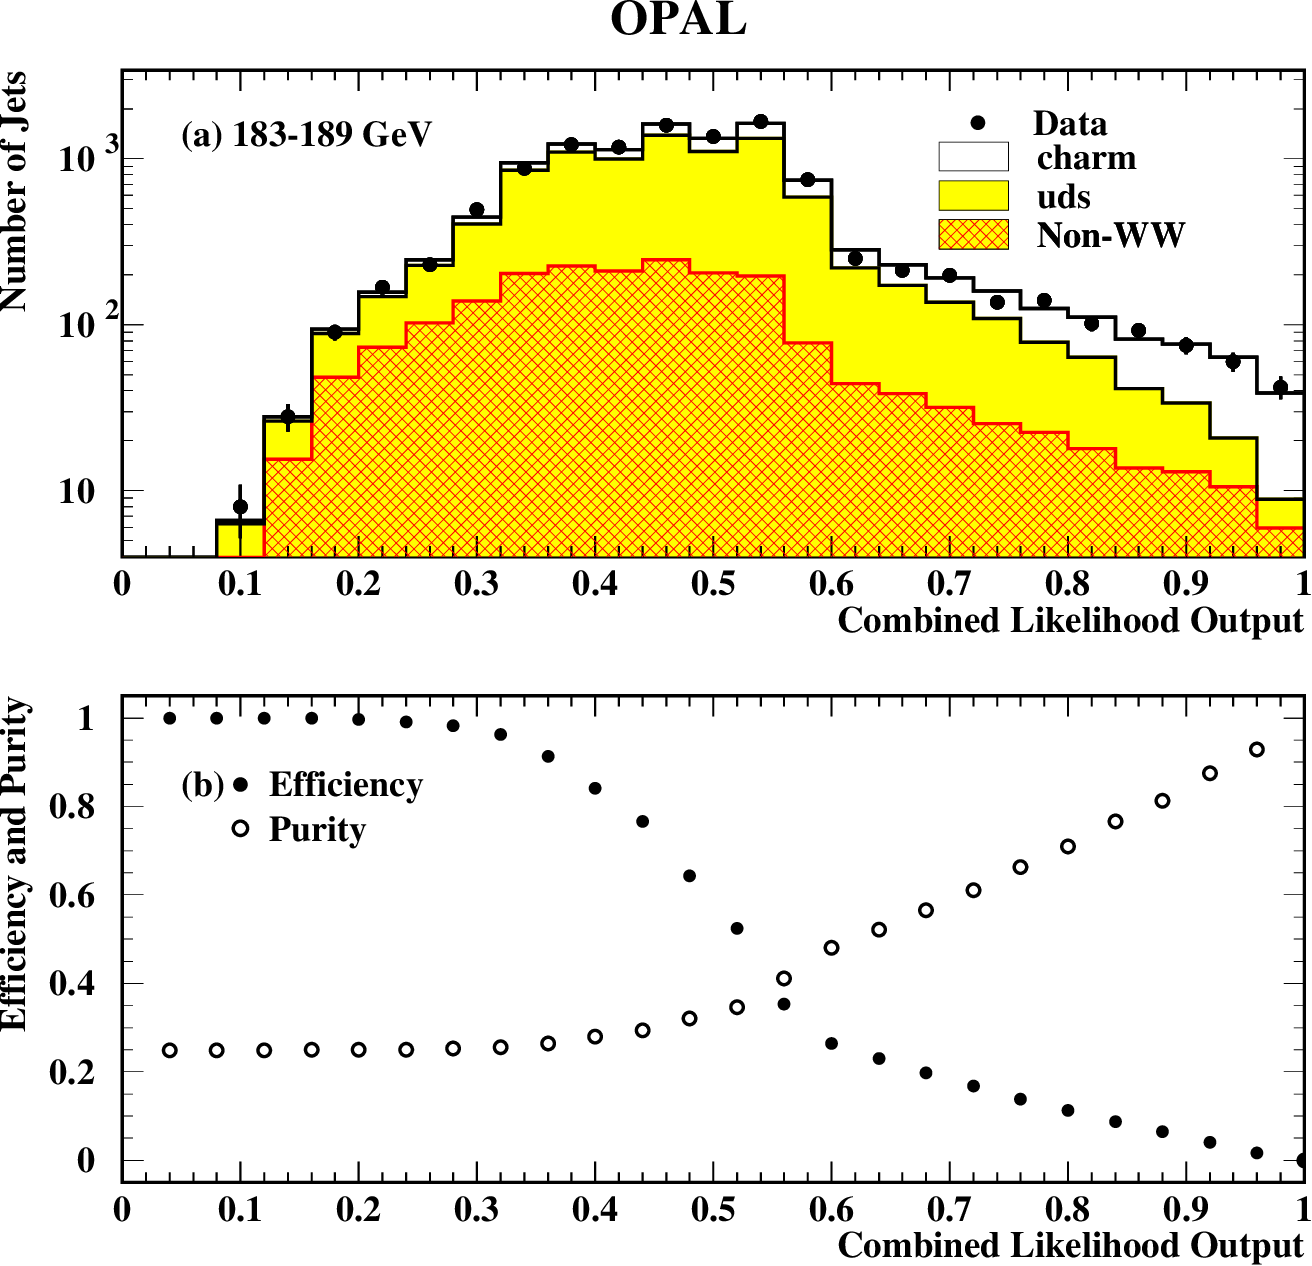
\includegraphics[width=\linewidth]{fig//chap02-theory/opal.png}
         \caption{OPAL: Output of the combined likelihood used to tag charm hadrons at 183–189 \GeV. \\\\}
    \end{subfigure}
     \hfill
     \begin{subfigure}{0.46\linewidth}
         \centering
        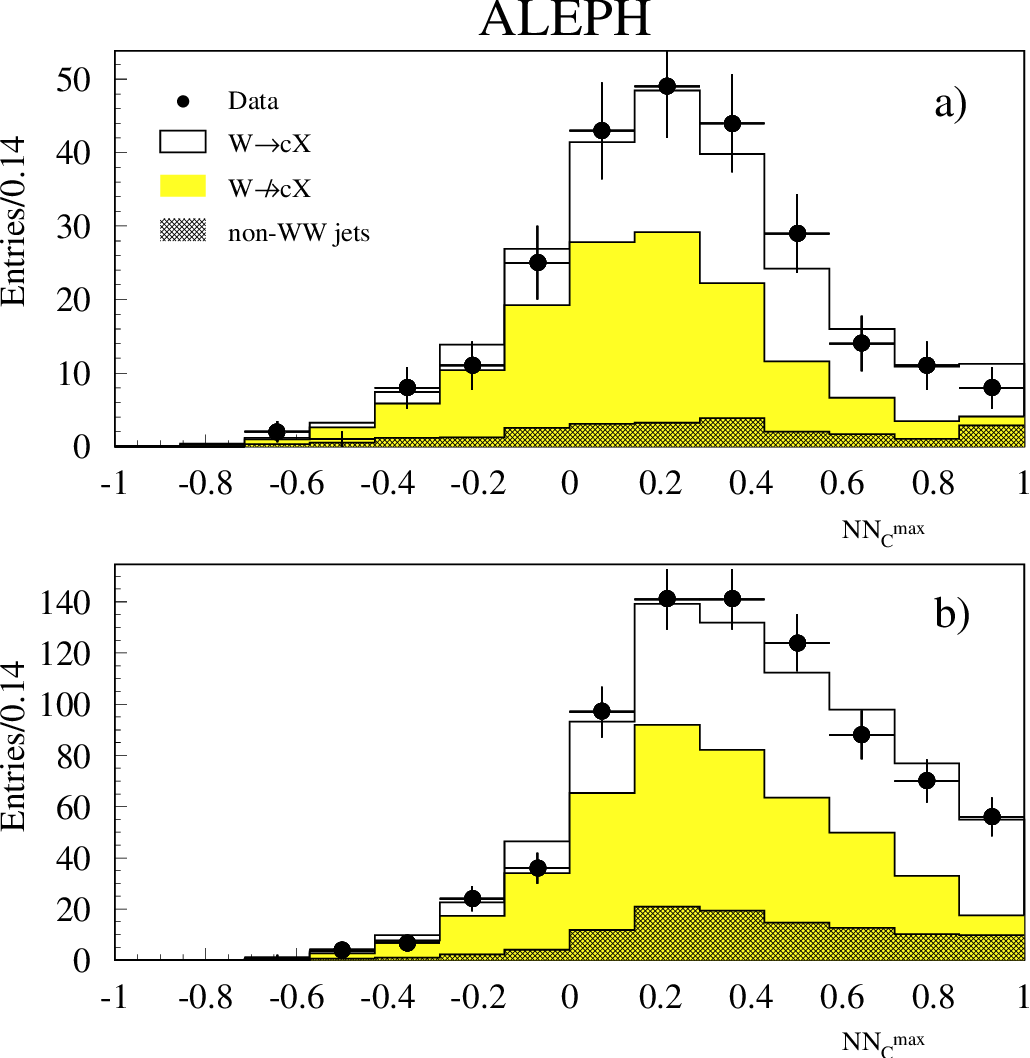
\includegraphics[width=\linewidth]{fig//chap02-theory/aleph.png}
         \caption{ALEPH: Maximum c tagging NN score for the dijet pairs. In the top panel there are the semileptonic WW pairs, in the bottom panel there are the fully hadronic}
     \end{subfigure}
        \label{fig:rc_lep}
\end{figure}
\vspace{-0.5cm}
\paragraph*{Direct measure of $|V_{cs}|$}
The $V_{cs}$ CKM element was measured directly from W decays by the DELPHI collaboration, using semileptonic and fully hadronic decays of WW pairs measuring $r^{(cs)}$ \cite{Abreu1998MeasurementLEP2}.
\vspace{-0.5cm}
\begin{equation}
    r^{(cs)}=\frac{\Gamma(W\to cs)}{\Gamma(W\to q\bar{q})}=\frac{|V_{cs}|^2}{2}
\end{equation}
where, in the last step, the unitarity of the CKM matrix is assumed.\\
To discriminate the signal, DELPHI built a cs tagger $P_{cs}$ that relies on information from the vertex and tracking detectors and on particle identification obtained by exploiting the Cherenkov subdetectors.\\
\begin{minipage}{\linewidth}
\begin{minipage}{0.4\linewidth}
    The value of $V_{cs}$ was extracted fitting the $P_{cs}$ distribution of selected di-jet combinations by using the maximum likelihood method on a multinomial likelihood
    \\
    The direct determination of $|V_{cs}|$ was performed on just 100 W pairs collected in 1996, leading to a large total uncertainty of $\sim 40\%$\\
\end{minipage}
\hfill
\begin{minipage}{0.58\linewidth}
    \vspace{-0.5cm}
    \begin{figure}[H]
        \centering
        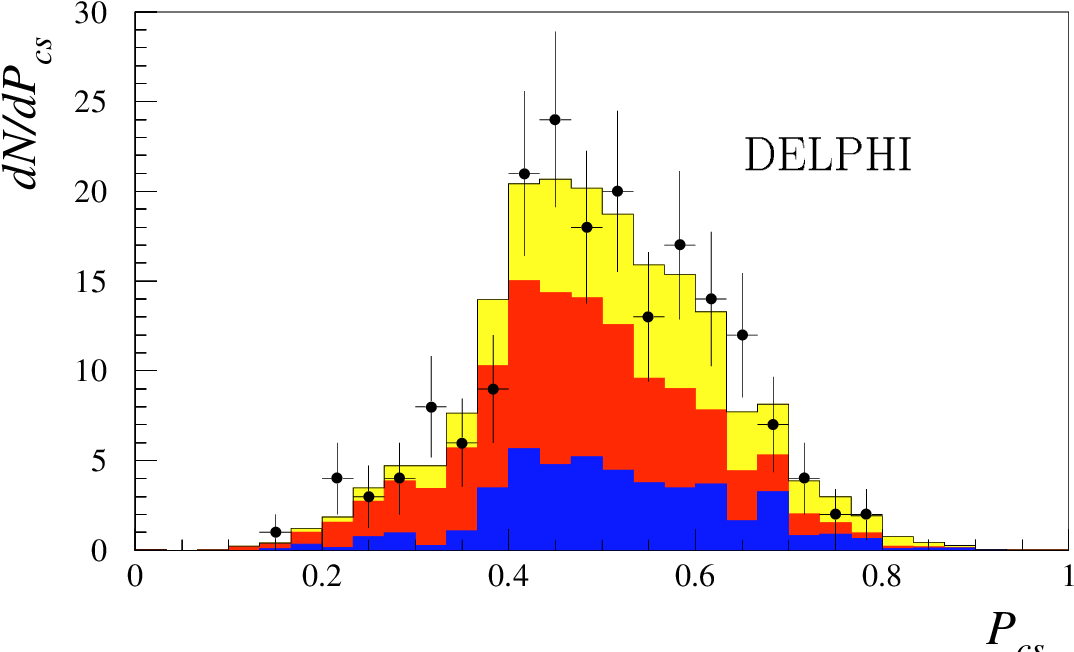
\includegraphics[width=\linewidth]{fig//chap02-theory/delphi.png}
        \caption{$P_{cs}$ spectra. The yellow is $W\to cX$, the red $W\to uX$, and the blue the background}
        \label{fig:enter-label}
    \end{figure}
\end{minipage}
    
\end{minipage}
However, for the first time, DELPHI was able to provide a determination of $|V_{cs}|$ dominated by the statistical uncertainties and not dependent on theoretical systematics.
\begin{align}
    |V_{cs}|&=0.94^{+0.32}_{-0.26}  \text{ (stat)} \pm 0.13 \text{ (syst)} & \text{(DELPHI)}
\end{align}





\subsection{$|V_{cb}|$ with LHC data}
This work aims to access the $|V_{cb}|$ element through the direct decay of a \PW boson at $\sqrt{s}=13 TeV$ with the recorded luminosity of the RunII.\\
\\
At LHC, in all the RunII, more than 8 billion single W bosons and more than 16 million WW pairs were produced: of these, more than 5 billion W bosons decay hadronically, which means that more than 2 million cb quark pairs can be obtained from the inclusive decay of \PW bosons, exploiting the advanced b tagging capabilities of the modern experiments. \\
Despite that, contrary to any electron-positron collider, an inclusive measurement of $\PW \to cb$ at a hadron collider would be an impossible task due to the large QCD background.\\
\\
To avoid it, it is possible to exploit the semileptonic decay of top pairs and use the lepton to trigger the event and the hadronic \PW decay to measure the $\PW \to cb$ branching fraction.\\
As lepton $\ell$, we will only consider muons and electrons, due to the lower reconstruction efficiency of $\tau$s, that decay hadronically in the $64.8\%$ of cases.
\\
\\
The value of $|V_{cb}|$ can be extracted from the ratio of branching fractions in which the hadronic \PW decays into c and b quarks over the  \PW hadronic branching fraction
\begin{equation}
\begin{gathered}
    R_{cb}=\frac{\Gamma\left(\ttbar \to b\ell \nu\; b cb\right)}{\Gamma\left(\ttbar \to b\ell \nu\; b q\bar{q}\right)}=\\ =\frac{|V_{cb}|^2}{|V_{ud}|^2+|V_{us}|^2+|V_{ub}|^2+|V_{cd}|^2+|V_{cs}|^2+|V_{cb}|^2}
\end{gathered}
\end{equation}
and if we assume the unitarity of the CKM matrix
\begin{equation}
    R_{cb}=\frac{|V_{cb}|^2}{2}
\end{equation}

The determination of $|V_{cb}|$ through direct \PW decays allows us to provide a new determination of $|V_{cb}|$ at a new energy scale ($\sqrt{s}=m_{\PW}$), avoiding complications and theoretical uncertainties due to non-perturbative QCD.\\
The statistic provided by the RunII does not allow to reach the current precision of $\sim2 \%$ on $|V_{cb}|$ that was obtained observing the semileptonic decays of $B$ mesons, but, despite that, it gives us an opportunity to tackle the $|V_{cb}|$ puzzle with a novel strategy.\\
The main sources of systematic uncertainties are the b/c tagging uncertainties, but the ratio of branching fractions should allow some cancellations.

\subsection{The Top quark}
The top quark is the heaviest particle of the standard model, discovered at Fermilab in 1995 by the CDF and the D0 collaborations \cite{Abe1995ObservationFermilab,Abe1995ObservationFermilab}.
Its lifetime, $\sim 10^{25}s$, is less than the hadronization timescale ($\sim 10^{-23}s$), making it the only quark that can decay freely \cite{Bigi1995TheHadrons}.
\\
\\
The top quark decays through weak interactions through the channel $\PQt \to \PW q$ and, due to its mass of $m_{\PQt} \simeq 173 \GeV$, the top quark is also the only particle that can decay into an on-shell $\PW$ boson.\\
Furthermore, the V-A structure of the weak interactions makes 
the kinematics of the top decay is strongly dependent on the polarization of the top quark.
\\
The final states that can be observed are:
\begin{itemize}
    \item $\PQt \to \PW^+ q^d_i \to q^d_1 q_2 \bar{q}_3 $ with a branching ration of $\simeq 68\%$
    \item $\PQt \to \PW^+ q^d_i \to q^d_1 \bar{\ell} \PGnl$ with a branching ratio of $\simeq 32\%$
\end{itemize}
The $q_i^d$ is a down-type quark and the branching fractions of the decay to the three different quarks is
\begin{equation}
\frac{\Gamma(\PQt \to \PW^+ q_i^d)}{\Gamma(\PQt \to \PW^+ q^d)} = |V_{\PQt i}|^2
\end{equation}
so the top quark decays to a \PW boson and a \PQb quark with a branching fraction closer to 100\%.
\paragraph*{Decay of top quark pairs}\hspace{0.1cm}\\
\begin{minipage}{\linewidth}
    \vspace{0.5cm}
    \begin{minipage}{0.45\linewidth}
        \raggedright
            \centering
            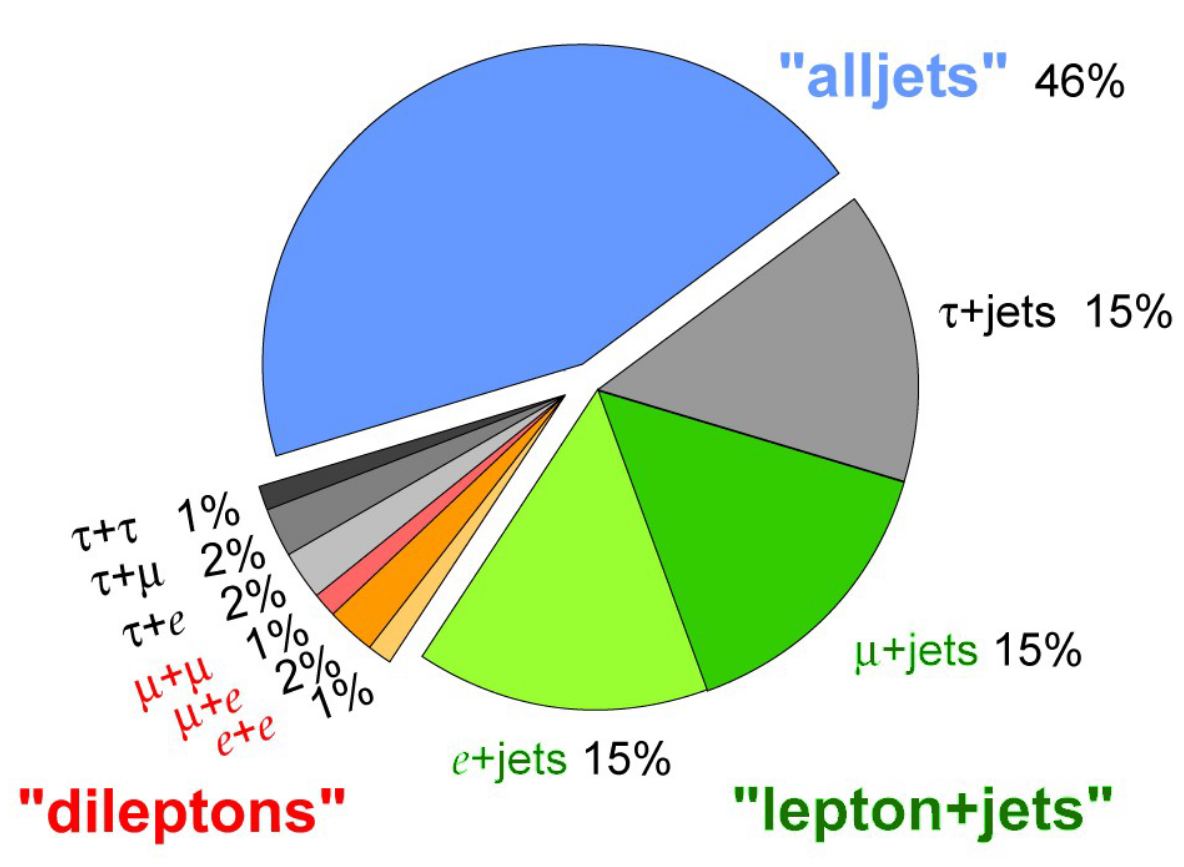
\includegraphics[width=\linewidth]{fig//chap02-theory/ttbr.png}
            \captionof{figure}{Top pair branching fractions}
            \label{fig:ttbr}
    \end{minipage}
    \hfill
    \begin{minipage}{0.5\linewidth}
        \raggedright
        Neglecting the decay of the top quark into down and strange quarks, the branching fractions of the \ttbar decay are:
        \begin{itemize}
            \item 45.5\% \textbf{Fully hadronic} $\ttbar \to \bbbar q \bar{q} q \bar{q}$. 
            \item 43.9\% \textbf{Semi leptonic} $\ttbar \to \bbbar q \bar{q} \ell \PGnl$
            \item 10.6\% \textbf{Di-leptonic} $\ttbar \to \bbbar \ell \PAGnl  \bar{\ell} \PGnl$
        \end{itemize}
        The branching ratio of the flavors of the $q_i\bar{q_j}$ pairs generated by \PW decays is given by the respective CKM elements $|V_{ij}|^2/2$.
    \end{minipage}

\end{minipage}



\subsection{Top pairs production at LHC}
In a hadron collider, top quarks are mainly produced in $\ttbar$ pairs via gluon-gluon fusion (ggF) $gg \to \ttbar$ or quarks annihilation ($\PQq\bar{\PQq} \to \ttbar$).
\begin{figure}[h!]
    \centering
    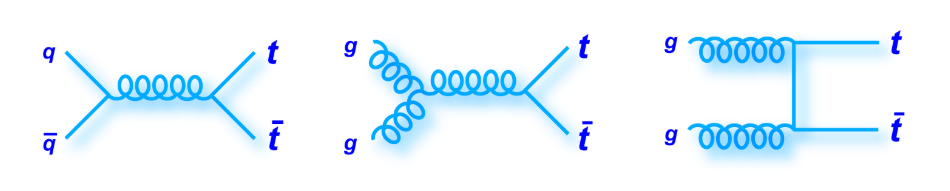
\includegraphics[width=0.8\linewidth]{fig//chap02-theory/ttbar.png}
    \caption{Tree level Feynman diagrams of $\ttbar$ production via gluon-gluon fusion (middle, right) and quark-antiquark annihilation (left)}
    \label{fig:tt_prod}
\end{figure}\\
The protons that collide in the LHC can be described by the parton model \cite{Feynman1969TheEnergies}.\\
Each proton is composed by three valence quarks (uud) and a sea of quarks, anti-quarks, and gluons generated by the QCD activity in the hadron.\\ 
The elements that compose the proton are called “partons” and each parton carries a fraction $x_i$ of the proton momentum.\\
The so-called Bjorken variable $x_i$ follows a statistical distribution, the parton distribution functions (PDFs) $f(x,Q^2)$, that depends on the type of parton and the proton momentum.\\
The equations that describe the evolution of the PDFs at the different energy scales are the Dokshitzer–Gribov–Lipatov–Altarelli–Parisi (DGLAP) equations \cite{Altarelli1977AsymptoticLanguage,Gribov1972DeepTheory,Dokshitzer1977CalculationChromodynamics.} but the PDFs can't be computed a priori, they have to be extracted from experimental data.
At low energies, the PDFs are dominated by the presence of valence quarks, but the contribution of gluons and non-valence quarks increases with the proton energy as shown in \Fig{fig:pdf}.
\\
\begin{figure}[h!]
    \centering
    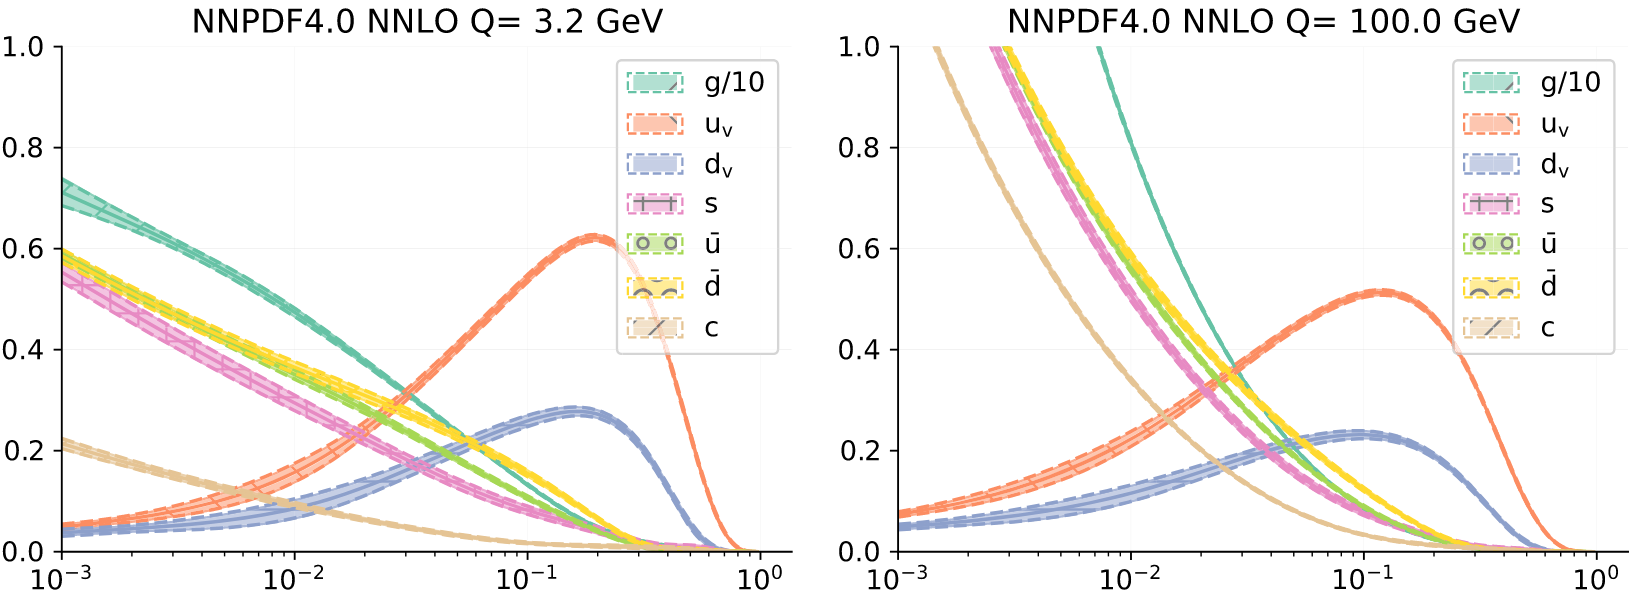
\includegraphics[width=1\linewidth]{fig//chap02-theory/pdf.png}
    \caption{$xf(x,Q^2)$ values for the NNPDF 4.0 NNLO PDFs set at $Q=3.2\GeV$ (left) and $Q=100 \GeV$ (right) presented by the NNPDF collaboration \cite{Ball2022TheAccuracy}. }
    \label{fig:pdf}
\end{figure}
\\
To compute the inclusive $\ttbar$ production cross-section at a hadron collider, the parton-level cross-section has to be convolved with the PDFs
\begin{equation}
    \sigma_{\mathrm{t\bar{t}}}=\sum_{i,j=q,\overline{{{q}}},g}\int d x_{i}d x_{j}f_{i}(x_{i},Q^{2})f_{j}(x_{j},Q^{2})\cdot\hat{\sigma}_{i j\rightarrow \ttbar}(x_i,x_j)
\end{equation}
where the sums run over the type of partons (quarks, antiquarks, and gluons).
The energy in the center of mass at LHC is $\sqrt{s}=13 \TeV$ and the predominant $\ttbar$ production channel is the ggF with a branching ratio of $\simeq 90\%$.\\
The total $\ttbar$ production cross-section computed at the $\mathcal{O} (\alpha_S^4)$ order of accuracy using the program \Toppp \cite{Czakon2014Top++:Colliders} and assuming $m_t=172.5 \pm 1.0 \GeV$ is  \cite{TtbarNNLOTWiki}
\begin{equation}
    \sigma_\ttbar = 833.9^{+20.5}_{-30.0}\, ^{+23.2}_{-22.5}\pm 21.0\,  \text{pb}\; \; \left( \pm \text{Scale} \pm m_t \pm (\text{PDF}+\alpha_s ) \right)
\end{equation}
\paragraph*{Extra jets}
The emission of radiative gluons or quarks can cause the formation of additional collimated sprays of hadrons called jets (see sec. \ref{sec:jets}).\\
These events are suppressed by a factor $\alpha_s$ for each new additional vertex in the Feynman diagram.


%\newchap{The $|V_{cb}|$ CKM element}\label{sec:vcb}
\vspace{-1cm}
\minitoc
This work aims to access the $|V_{cb}|$ element through the direct decay of a \PW boson at $\sqrt{s}=13 TeV$ with the recorded luminosity of the RunII.
\vspace{-0.25cm}
\section{The $V_{cb}$ element}\label{sec:vcb}
\begin{minipage}{\linewidth}
    \begin{minipage}{0.43\linewidth}
        The $V_{cb}$ element plays an important role in the unitarity of the CKM matrix. The radius of the unitarity-clock, the green circle centered in the origin in \Fig{fig:triangle}, is proportional to the ratio $|V_{ub}/V_{cb}|$, so $V_{cb}$ normalize the whole triangle \cite{Ricciardi2019DeterminationV_cb}.\\
        \\
        $|V_{cb}|$ is measured from the semileptonic inclusive and exclusive $b \to c\ell\nu$
        decays but the parton level amplitude, which is proportional to $|V_{cb}|^2$, has to be corrected by introducing form factors to consider the contributions by strong interactions in the meson. 
    \end{minipage}
    \hfill
    \begin{minipage}{0.55\linewidth}
        \vspace{-2.1cm}
        \begin{figure}[H]
            \centering
            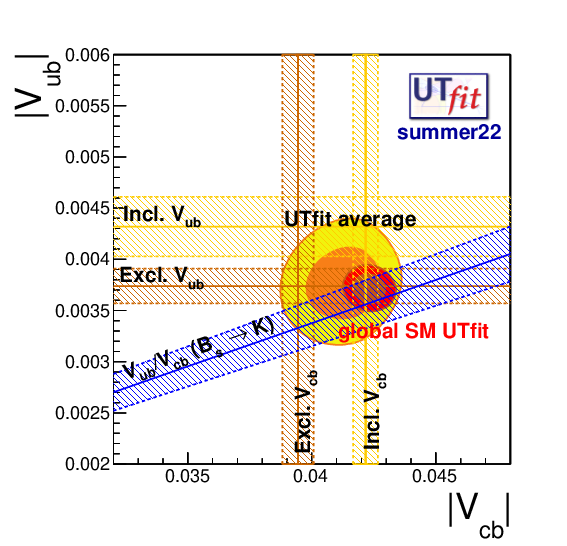
\includegraphics[width=\linewidth]{fig//chap02-theory/vubvcb.png}
            \caption{$|V_{cb}|$ and $|V_{ub}|$ global fit and averages of inclusive and exclusive measurements performed by the UTfit collaboration \cite{Bona2023NewScheme}}
            \label{fig:vcbvub}
        \end{figure}
    \end{minipage}
\end{minipage}\\
\\
These corrections inevitably lead to theoretical uncertainties that are of the same order as the experimental systematic uncertainties.\\
These issues also concern the $|V_{ub}|$ measurements.\\
A summary of the single measurements of the $|V_{cb}|$ element can be found in \cite{PDG_2022}.
\subsection{$|V_{cb}|$ from semileptonic B meson decays}
\paragraph*{Inclusive measurement}
The inclusive channel $B\to X_c \ell \nu$ is less model dependent than the exclusive one \cite{Smith2005DeterminationSpectra}.
The QCD contributions can be included by adding two terms in the amplitude: a perturbative term and a non-perturbative term.
\begin{equation}
    \Gamma(B\rightarrow X_c\ell\nu)=\frac{G_{F}^{2}m_{b}^{5}|V_{c b}|^{2}}{192\pi^{3}}[1+P(\alpha_{s},\mu,m_{b}/m_{c})+N(m_b,m_c,\mu_\pi^2,\mu_G^2,\rho_D^2,\rho_{LS}^3)]
\end{equation}
The QCD corrections are computed using the so-called Operator Product Expansion (OPE). OPE allows us to express the widths and moments of the kinematic distributions as a double expansion in $\alpha_S$ and $\Lambda_{QCD}/m_b$. These corrections are actually known up to the third order in $\Lambda_{QCD}/m_b$ \cite{Alberti2016TheVcb}.\\
This expansion depends on other parameters defined in the framework of the heavy quark effective field theory (HQET) that can be constrained through the study of other observables like the lepton energy, the transferred momentum or the hadronic mass \cite{Smith2005DeterminationSpectra} so the final fit has to be performed on an order of $\mathcal{O}(100)$ of observables.\\
The uncertainties of the inclusive measurements of $|V_{cb}|$ are  $\simeq 2\%$, mainly driven by theoretical uncertainties related to the determination of the HQET parameters \cite{Alberti2016TheVcb}.\\
The average of the inclusive measurements is \cite{Bordone2021ThreeVcb}
\begin{equation}
    |V_{cb}|\times10^3\text{ (incl)}=42.16\pm 0.50
\end{equation}

\paragraph*{Exclusive measurement}
The two main exclusive channels studied for $|V_{cb}|$ determination are the $\PAB \to D^* \ell \PAGnl$ and the $\PAB \to D \ell \PAGnl$.
The first channel was measured with an uncertainty of $\simeq 2\%$ with comparable contributions from theory and experiment, while the latter was measured with an uncertainty of the $\simeq 3\%$ but recently
some questions about the form factor parametrization were raised.\\
The exclusive measurement requires knowing six form factors that can be computed using lattice QCD (LQCD) techniques. In the limit of heavy quarks, the six form factors collapse into a single one, and corrections to the $m_b \to \infty$ limit can be obtained through the HQET framework \cite{PDG_2022}.\\
The average of the exclusive measurements is \cite{Bona2023NewScheme}
\begin{equation}
    |V_{cb}|\times10^3\text{ (excl)}=39.44\pm 0.63
\end{equation}

\paragraph*{The $|V_{cb}|$ puzzle}
The inclusive and exclusive measurements of the $V_{cb}$ element have always been incompatible as shown in \Fig{fig:vcbvub}.\\
Recently, a revision of the techniques involved in the calculations of the QCD contributions has narrowed the gap, but the $V_{cb}$ puzzle is still unresolved \cite{Bona2023NewScheme}: indeed the current determinations show a 7\% difference from each other.\\ 
Combining the measurements with a $\chi^2$ fit, the best-fit value is $|V_{cb}|_{\text{best}}=41.10$ that leads to a chi-square of $\chi^2=11.35$, corresponding to a p-value $p=7.2 \cdot 10^{-4}$, \ie to $\sim 3.3\sigma$.\\
\\
The determination of $|V_{cb}|$ through direct \PW decays would allow us to provide a new determination of $|V_{cb}|$ at a new energy scale ($\sqrt{s}=m_{\PW}$), avoiding complications and theoretical uncertainties due to non-perturbative QCD, tackling the $|V_{cb}|$ puzzle with a novel strategy.
\section{CKM measurements from hadronic W decays}
\subsection{LEP2 measurements}
The Large Electron-positron Collider (LEP) was an electron-positron collider that reached a peak energy in the center of mass of 209 GeV. It was built at CERN and is located in the tunnel that now hosts the LHC accelerator facility and started its physics program in 1989.\\
\\
The LEP2 physics program started in 1996, running at a center of mass energy  that was increased from 161\GeV to 209\GeV at the end of 1999, above the production threshold of WW pairs. 
In this period, each of the four LEP experiments, ALEPH, DELPHI, L3, and OPAL have collected  $\sim700 \text{pb}^{-1}$ of data above the WW pair production threshold, corresponding to over 10000 WW events per experiment \cite{Lu2008WLEP}.\\
\\
In this period, $\sim 10$ $\PW \to cb$ events per experiment were produced, making it impossible to provide a direct determination of $|V_{cb}|$ from inclusive \PW decays.\\
However, with more than 13000 hadronic W decays per experiment, the LEP experiments were able to access other elements in the charm sector of the CKM matrix.


\paragraph*{Rate of charm production}
ALEPH and OPAL performed a measure of the rate or $W\to cX$ decays on both semileptonic and fully hadronic WW pairs.
\begin{equation}
    R_c^W=\frac{\Gamma(W\to cX)}{\Gamma(W\to q\bar{q})}=\frac{|V_{cd}|^2+|V_{cs}|^2+|V_{cb}|^2}{|V_{cd}|^2+|V_{cs}|^2+|V_{cb}|^2+|V_{ud}|^2+|V_{us}|^2+|V_{ub}|^2}
\end{equation}
This is a unitarity test of the second row of the CKM matrix, indeed, if the unitarity hypothesis holds, it has to be $R_c^W=0.5$.
\\
\\
ALEPH performed the measurement extracting $R_c^W$ with a binned maximum-likelihood fit on the shape of the most c-tagged jet\cite{Barate1999ATag}.\\
The charm jet tagger was a feed-forward neural network with 12 variables as input that uses mainly information from charm lifetime, jet-shape properties, reconstruction of D mesons, and lepton identification.\\
\\
On the other hand, OPAL used a relative likelihood discriminant calculated for each jet to separate jets originating from charm quarks and jets from light quarks. This discriminant relies on jet and event shape properties, lifetime information, and lepton identification \cite{Abbiendi2000ADecays}.
\\
\\
The results of both experiments are consistent with the unitarity hypothesis with an uncertainty of $\sim 10\%$
\begin{equation}
\begin{aligned}
    R_c^W&=0.51 \pm 0.05 \text{ (stat)} \pm 0.03 \text{ (syst)} & \text{(ALEPH \cite{Barate1999ATag})}\\
    R_c^W&=0.481 \pm 0.042 \text{ (stat)} \pm 0.032 \text{ (syst)} & \text{(OPAL \cite{Abbiendi2000ADecays})}
\end{aligned}
\end{equation}\vspace{-0.001cm}
$R_C^W$ allow also an indirect measure of $|V_{cs}|$, subtracting the other $|V_{cx}|$ CKM elements in quadrature from $R_C^W$ obtained from other determinations.
\begin{equation}
\begin{aligned}
    |V_{cs}|&=1.00\pm0.11  \text{ (stat)} \pm 0.07 \text{ (syst)} & \text{(ALEPH \cite{Barate1999ATag})}\\
    |V_{cs}|&=0.969\pm0.058 & \text{(OPAL \cite{Abbiendi2000ADecays})}
\end{aligned}
\end{equation}
\begin{figure}[H]
    \begin{subfigure}{0.48\linewidth}
        \centering
         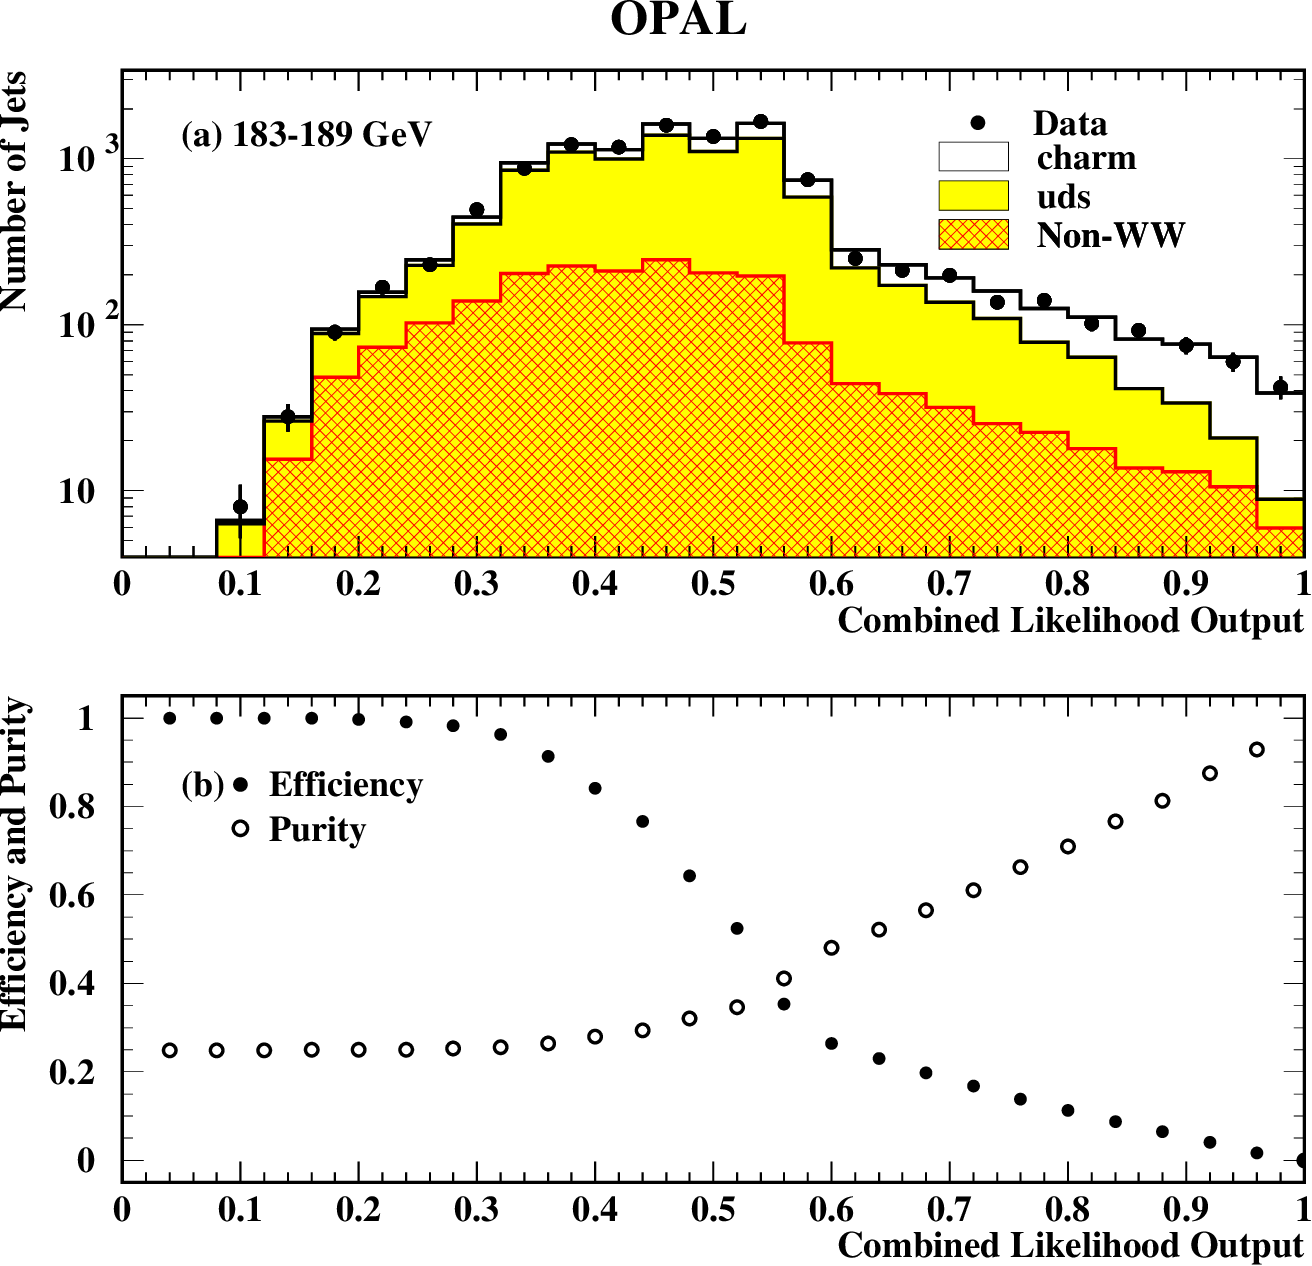
\includegraphics[width=\linewidth]{fig//chap02-theory/opal.png}
         \caption{OPAL: Output of the combined likelihood used to tag charm hadrons at 183–189 \GeV\cite{Abbiendi2000ADecays}.\\}
    \end{subfigure}
     \hfill
     \begin{subfigure}{0.475\linewidth}
         \centering
        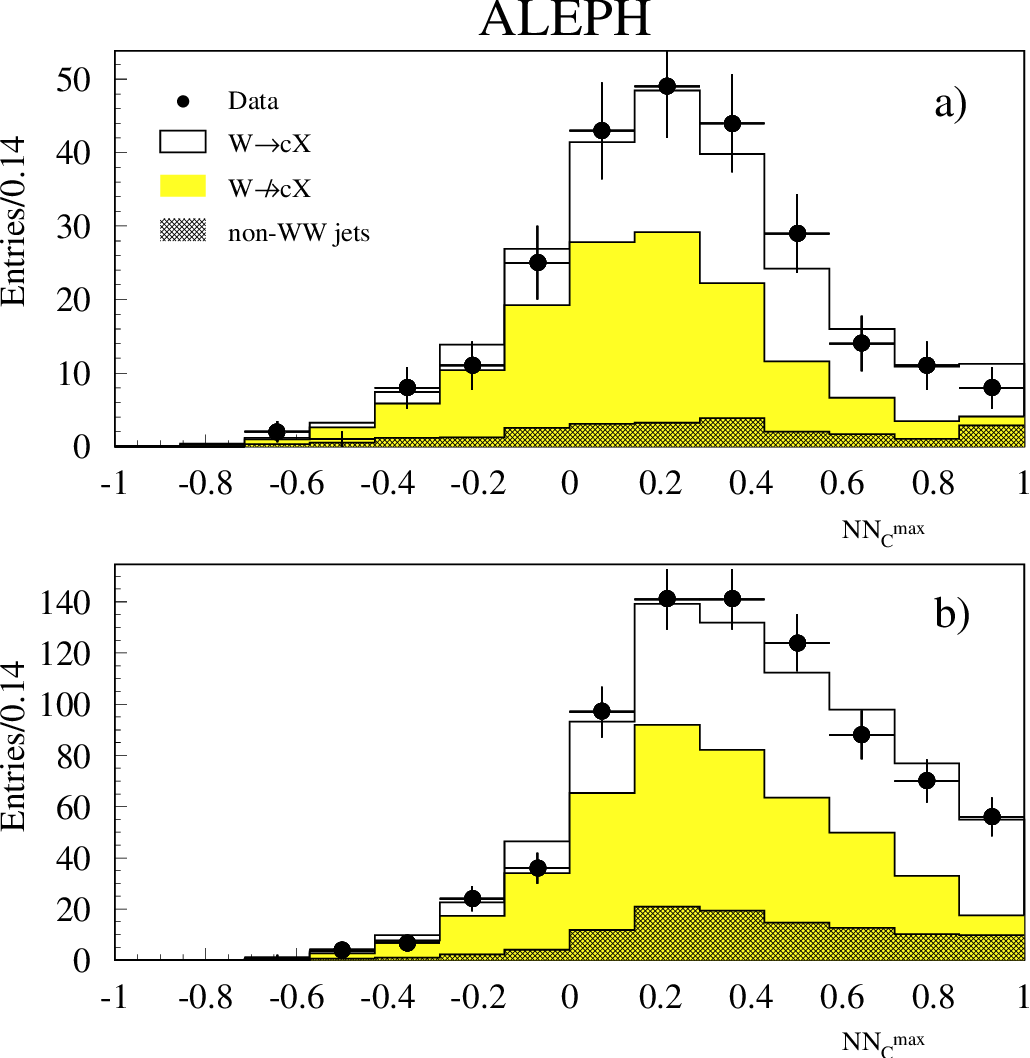
\includegraphics[width=\linewidth]{fig//chap02-theory/aleph.png}
         \caption{ALEPH: Maximum c tagging NN score for the dijet pairs. In the top panel there are the semileptonic WW pairs, in the bottom panel there are the fully hadronic \cite{Barate1999ATag}.}
     \end{subfigure}
        \label{fig:rc_lep}
\end{figure}
\vspace{-0.85cm}
\paragraph*{Direct measure of $|V_{cs}|$}
The $V_{cs}$ CKM element was measured directly from W decays by the DELPHI collaboration, using semileptonic and fully hadronic decays of WW pairs measuring $r^{(cs)}$ \cite{Abreu1998MeasurementLEP2}.
\vspace{-0.5cm}
\begin{equation}
    r^{(cs)}=\frac{\Gamma(W\to cs)}{\Gamma(W\to q\bar{q})}=\frac{|V_{cs}|^2}{2}
\end{equation}
where, in the last step, the unitarity of the CKM matrix is assumed.\\
To discriminate the signal, DELPHI built a cs tagger $P_{cs}$ that relies on information from the vertex and tracking detectors and on particle identification through RICH detectors.\\
\begin{minipage}{\linewidth}
\begin{minipage}{0.4\linewidth}
    \vspace{-1cm}
    The value of $V_{cs}$ was extracted fitting the $P_{cs}$ distribution of selected di-jet combinations by using the maximum likelihood method on a multinomial likelihood.
    \\
    The direct determination of $|V_{cs}|$ was performed on just 100 WW pairs collected in 1996, leading to a large statistical uncertainty of $\sim 30\%$\\
\end{minipage}
\hfill
\begin{minipage}{0.58\linewidth}
    \begin{figure}[H]
        \centering
        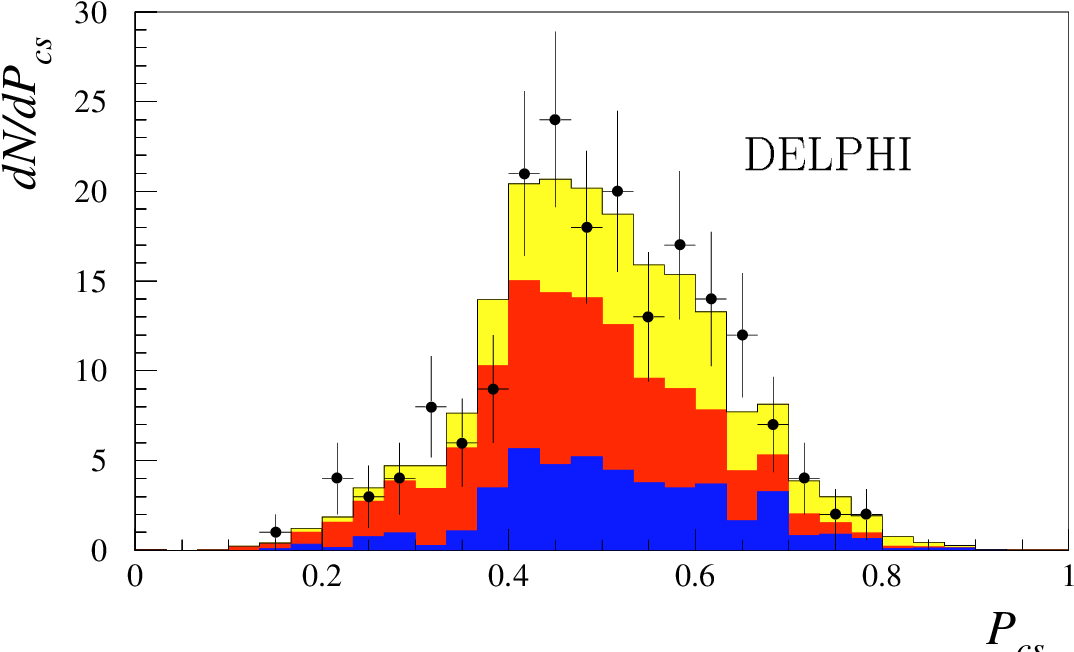
\includegraphics[width=\linewidth]{fig//chap02-theory/delphi.png}
        \caption{$P_{cs}$ distribution. The yellow is $W\to cX$ process, the red $W\to uX$, and the blue is the background \cite{Abreu1998MeasurementLEP2}.}
        \label{fig:enter-label}
    \end{figure}
\end{minipage}
\end{minipage}
\\
However, for the first time, DELPHI was able to provide a direct determination of $|V_{cs}|$ dominated by the statistical uncertainties and not dependent on theoretical systematics.
\begin{equation}
\begin{aligned}
    |V_{cs}|&=0.94^{+0.32}_{-0.26}  \text{ (stat)} \pm 0.13 \text{ (syst)} & \text{(DELPHI \cite{Abreu1998MeasurementLEP2})}
\end{aligned}
\end{equation}


\subsection{$|V_{cb}|$ with LHC data}
At LHC, in all the RunII, more than 26 billion single W bosons were produced: of these, more than 17 billion W bosons decay hadronically, which means that more than 14 million cb quark pairs can be obtained from the inclusive decay of \PW bosons.\\
Despite that, contrary to any electron-positron collider, an inclusive measurement of $\PW \to cb$ at a hadron collider would be an impossible task due to the large QCD background.\\
\\
To avoid it, it is possible to exploit the semileptonic decay of WW pairs and use the lepton to trigger the event and the hadronic \PW decay to measure the $\PW \to cb$ branching fraction.\\
As lepton $\ell$, we will only consider muons and electrons, due to the lower reconstruction efficiency of $\tau$s, that decay hadronically in the $64.8\%$ of cases.
\\
\\
The value of $|V_{cb}|$ can be extracted from the ratio of branching fractions in which the hadronic \PW decays into c and b quarks over the  \PW hadronic branching fraction
\begin{equation}
\begin{gathered}
    R_{cb}=\frac{\Gamma\left(\PW\PW \to \ell \nu\; cb\right)}{\Gamma\left(\PW\PW \to \ell \nu\; q\bar{q}\right)}=\\ =\frac{|V_{cb}|^2}{|V_{ud}|^2+|V_{us}|^2+|V_{ub}|^2+|V_{cd}|^2+|V_{cs}|^2+|V_{cb}|^2}
\end{gathered}
\end{equation}
and if we assume the unitarity of the CKM matrix
\begin{equation}
    R_{cb}=\frac{|V_{cb}|^2}{2}
\end{equation}

This kind of measure will be limited mainly by the b and c tagging systematic uncertainties, but the ratio of branching fractions should allow some cancellations.
\paragraph*{WW production}
At an energy of the center of mass of $\sqrt{13 \TeV}$, the direct WW production cross section is $\sigma_{pp\to\PW\PW}\sim118 \text{pb}$, which means that in all the RunII, more than 16 million of WW pairs were produced directly.\\
However, at LHC, the production cross-section of $\ttbar$ pairs is $\sim 7$ times greater than the direct WW production cross-section with $\sigma_{pp\to \ttbar}\sim832\text{pb}$ and, since the top quark decays in one b quark plus a \PW boson, we can exploit di-top decays as a \PW\PW factory.
\newpage
\paragraph*{Decay of WW pairs}\hspace{0.1cm}\\
\begin{minipage}{\linewidth}
    \vspace{0.5cm}
    \begin{minipage}{0.42\linewidth}
        \raggedright
            \centering
            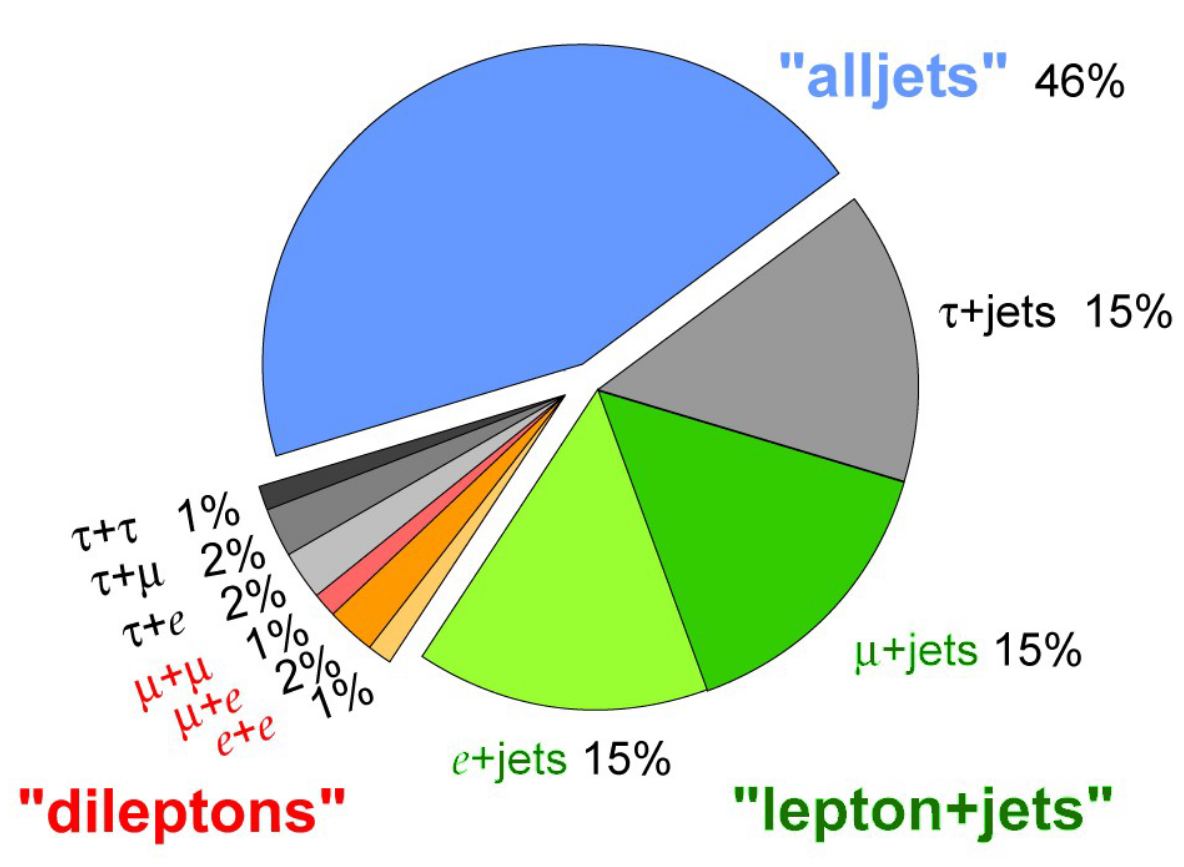
\includegraphics[width=\linewidth]{fig//chap02-theory/ttbr.png}
            \captionof{figure}{\PW pair decay branching fractions}
            \label{fig:ttbr}
    \end{minipage}
    \hfill
    \begin{minipage}{0.56\linewidth}
        \vspace{-1.1cm}
        \raggedright
        Since the branching fraction of the W decay are:
        \begin{itemize}
            \item 32.6\% \textbf{Hadronic} $\PW \to q\bar{q}$
            \item 67.4\% \textbf{Leptonic} $\PW \to \ell\nu$
        \end{itemize}
        the branching fractions of the $\PW^+\PW^-$ decay are:
        \begin{itemize}
            \item 45.5\% \textbf{Fully hadronic} $\PW\PW \to q \bar{q} q \bar{q}$. 
            \item 43.9\% \textbf{Semi leptonic} $\PW\PW \to q \bar{q} \ell \PGnl$
            \item 10.6\% \textbf{Di-leptonic} $\PW\PW \to \ell \PAGnl  \bar{\ell} \PGnl$
        \end{itemize}
        The branching ratio of the flavors of the $q_i\bar{q_j}$ pairs generated by \PW decays is given by the respective CKM elements $|V_{ij}|^2/2$.
    \end{minipage}

\end{minipage}
\\
\\
Since more than 110 million WW pairs were produced in the RunII through di-top decays, around 40000 $\PW \to cb$ events were produced in the $\ttbar$ semileptonic channel, while the amount of cb events produced by the semileptonic decay of directly produced WW pairs is around 6000.\\
\\
The amount of cb events provided by $\ttbar$ semileptonic decays in the RunII allows us to provide a new determination of $|V_{cb}|$ that, in case of a perfect selection, can reach the 0.5\% statistical precision, that is a huge improvement with respect the current 7\% difference between the current inclusive and exclusive determination obtained through the semileptonic decay of B mesons.\\
However, the separation between signal and background, which relies mainly on the b/c-tagging capabilities of the experiment, must be evaluated, along with the b/c-tagging systematic uncertainties.

\begin{table}[H]
    \centering
    \begin{tabular}{c|c|c|c|c}
        \toprule
        \multicolumn{5}{c}{$\PW \to cb$ events}\\
        \midrule
        \midrule
        \textbf{W} &  \multicolumn{2}{c|}{\textbf{WW}} & \multicolumn{2}{c}{$\bm{t\bar{t}}$} \\
        \midrule
          $1.4 \cdot 10^7$&  \multicolumn{2}{c|}{$1.8 \cdot 10^4$}  &  \multicolumn{2}{c}{$1.2 \cdot 10^5$} \\
        \midrule
        \textbf{Had} & \textbf{diHad} & \textbf{semiLept} & \textbf{diHad} & \textbf{semiLept}\\
        \midrule
         $1.4 \cdot 10^7$ & $1.2\cdot 10^4$ & $5.8 \cdot 10^3$ & $8.0 \cdot 10^4$ & $4.0\cdot 10^4$ \\
         \bottomrule

    \end{tabular}
    \caption{Amount of $\PW \to cb$ events produced per experiment in all the RunII at LHC for each process.}
    \label{tab:my_label}
\end{table}
%%!TEX root = ../thesis.tex
\newchap{The CMS experiment at LHC}\label{sec:CMS}
\vspace{-1cm}
\minitoc

CERN is the largest international particle physics research center in the world. It is located across the Franco-Swiss border in Meyrin, near Geneva, and was founded in 1954, after the end of World War II, by twelve European countries.\\
Today, more than 100 countries, 500 institutes, and 13000 users collaborate to the CERN activities.

\section{The Large Hadron Collider}
The CERN's major facility is the Large Hadron Collider (LHC), a proton-proton (pp) and ions collider that, with its lengths of 26.7 km and its energy in the center of mass of $\sqrt{s}=13.6\TeV$, is the largest and the most powerful particle accelerator ever built in the world.\\
As shown in \Fig{fig:cern}, the LHC is just the last stage of a chain of accelerators. The protons obtained from ionizing hydrogen are grouped in bunches through a quadrupole magnet and then are sent to a chain of accelerators that increase progressively the energy of the protons.
Before entering the LHC, the proton beam is split into two beam lines that travel in opposite directions and then are accelerated by radiofrequency (RF) cavities that are tuned to oscillate at 400MHz. In addition to RF cavities, quadrupoles are used to keep the beam focused and dipoles to bend the beam \cite{Bruning2004LHCReport}.\\
Once the beam is stabilized, the proton bunches collide in four different points where the experiments ATLAS, CMS, LHCb, and ALICE are located.\\
ATLAS (A Toroidal LHC ApparatuS) and CMS (Compact Muon Solenoid) are general-purpose detectors and are the ones that in the 2012 discovered the Higgs boson  \cite{Chatrchyan2012ObservationLHC,Aad2012ObservationLHC}, LHCb (LHC beauty) is a forward detector designed to study the physics of the B mesons and the matter-antimatter asymmetry and ALICE (A Large Ion Collider Experiment) is a detector devoted to the study of quark-gluon plasma and extreme phases of QCD matter through the analysis of lead ion collisions.
\begin{figure}[h!]
    \centering
    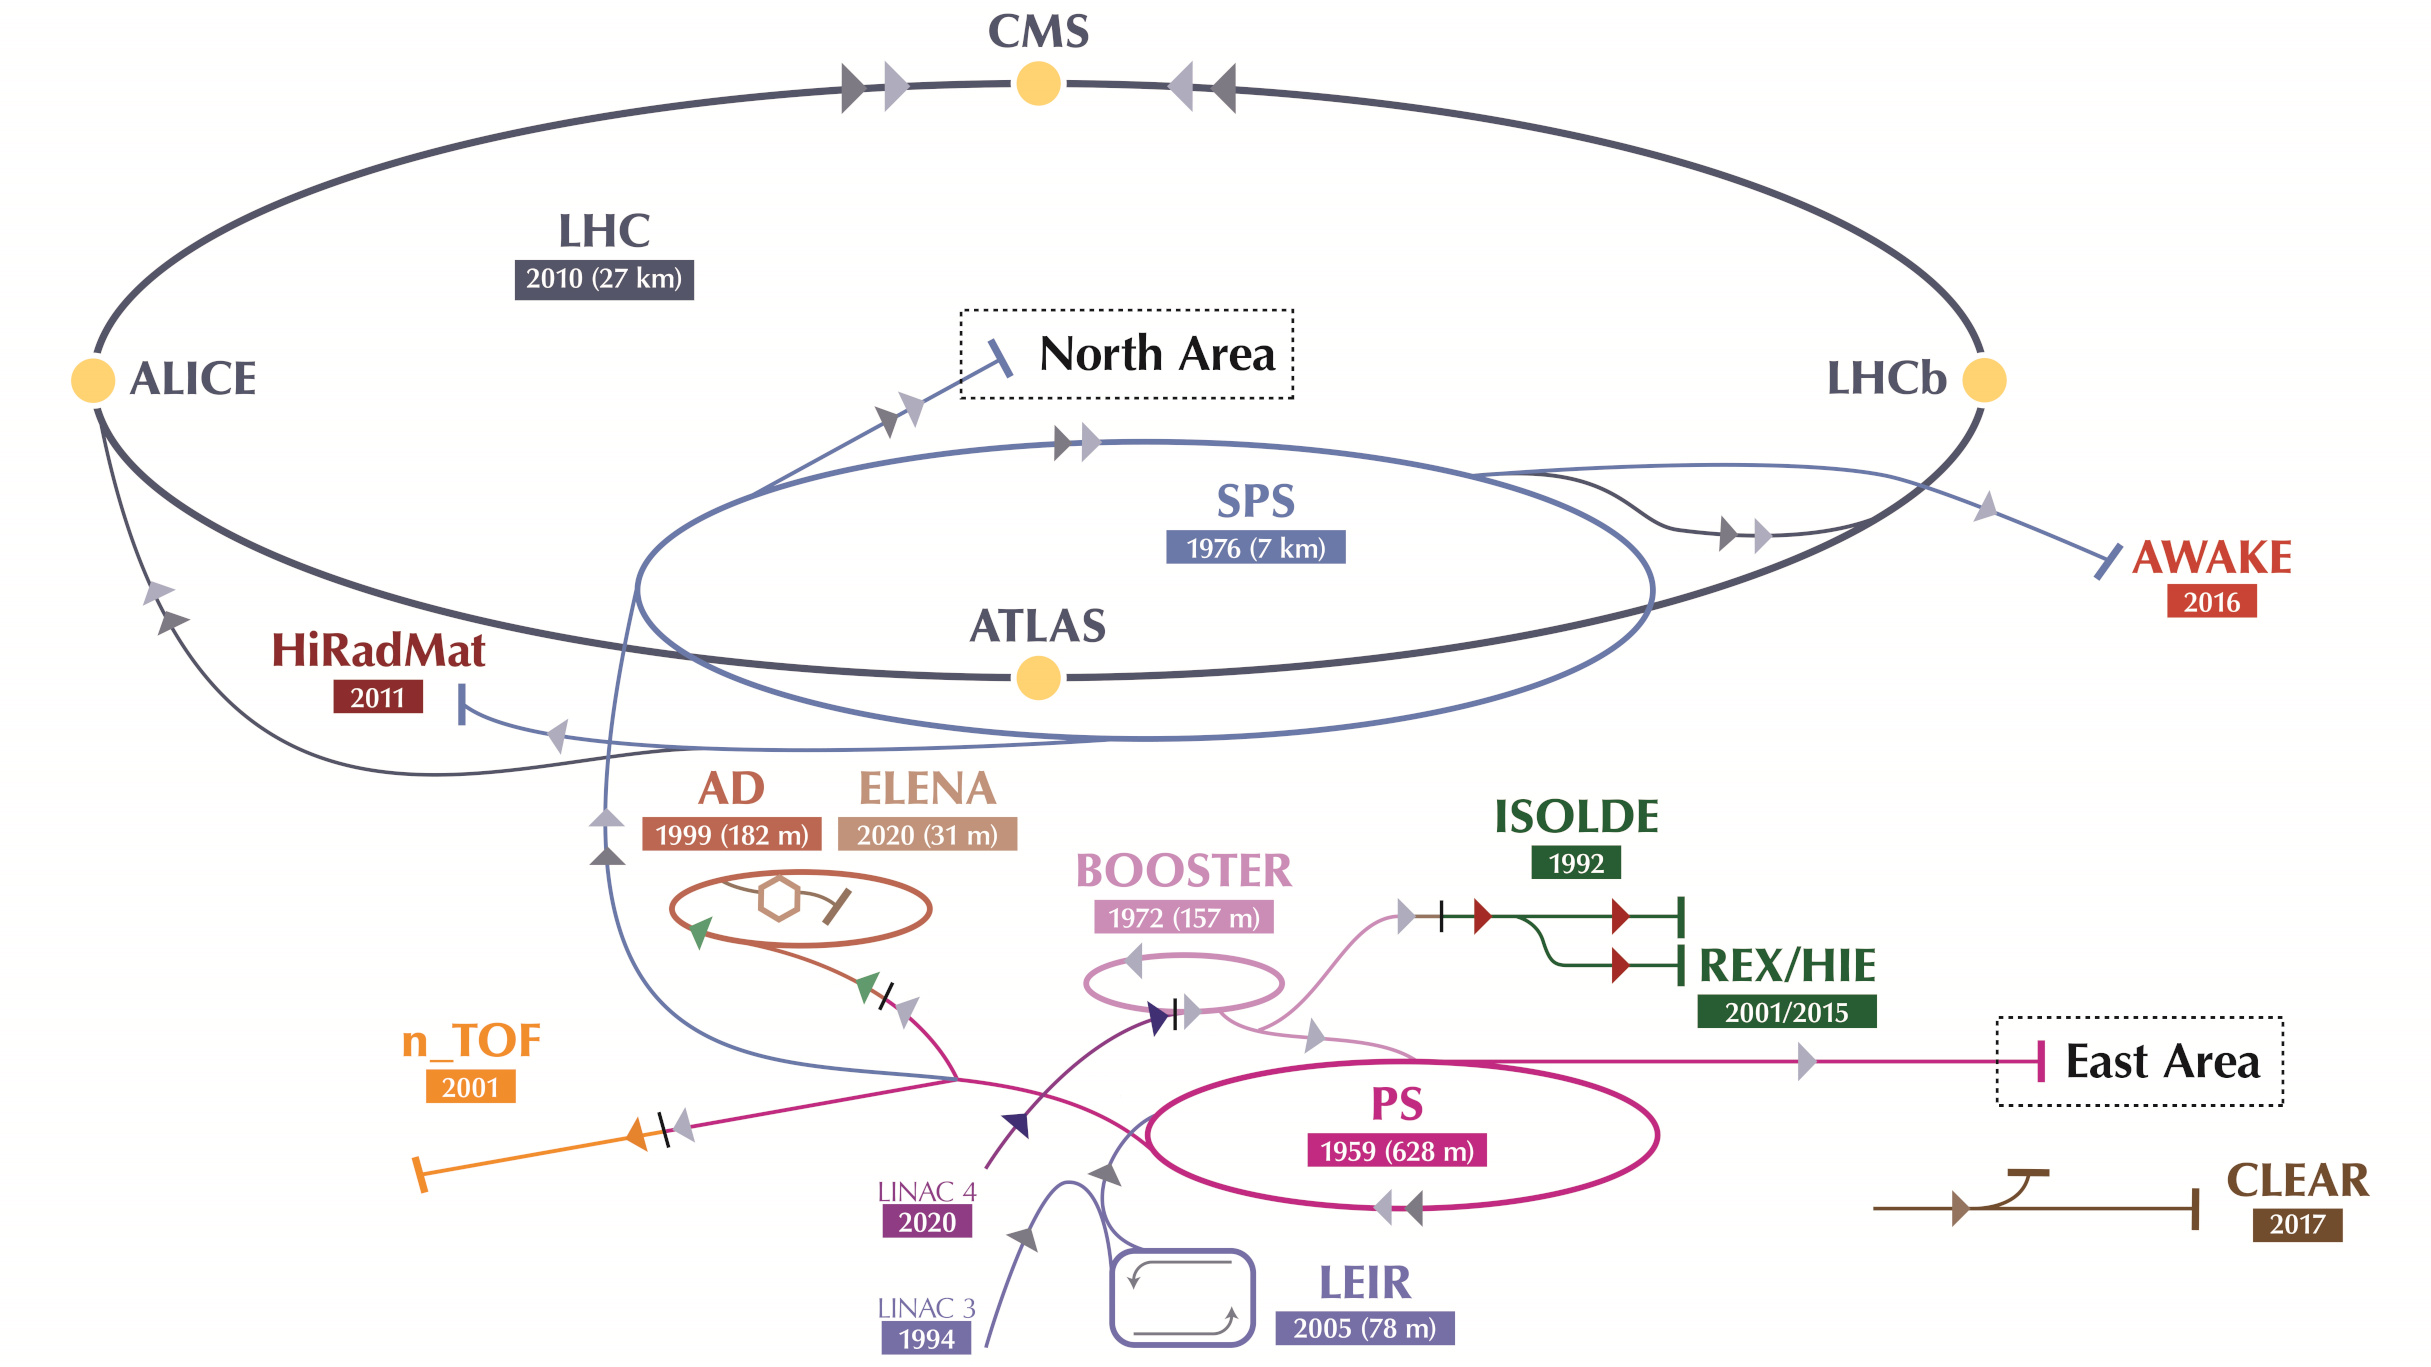
\includegraphics[width=\textwidth]{fig//chap03-cms/cern.jpg}
    \caption{CERN's accelerator complex. The accelerating chain is: LINAC2 (50 \MeV) $\to$ Booster (1.4\GeV) $\to$ Proton Synchrotron (PS) (26\GeV) $\to$ Super Proton Synchrotron (450\GeV) $\to$ LHC (13/14 \TeV). The intermediate accelerators also provide a proton beam to other smaller experiments and facilities. \cite{Panoramas}}
    \label{fig:cern}
\end{figure}

\paragraph*{Luminosity}
The \emph{instantaneous luminosity} is defined as the ratio between the event rate produced for a given process and its cross-section
\begin{equation}
    \mathcal{L} = \frac{\partial N}{\partial t} \frac{1}{\sigma} 
\end{equation}
and can be expressed also as a function of the beam parameters
\begin{equation}
    \mathcal{L}=\frac{N_{p}^{2}f\gamma_{r}}{4\pi\epsilon_{n}\beta\sp{\ast}}F\ 
\end{equation}
where $N_p$ is the number of protons per bunch, $f$ the bunch frequency, $\gamma_r$ the relativistic factor, and $\epsilon_n, \beta^*, F$ are geometrical factors that take into account the shape of the beam and the crossing angle between the two beams in the interaction point (IP).\\
These parameters depend on the so-called “filling scheme”, the chosen pattern of filled and empty bunch crossings used in a single fill.
A typical filling scheme is composed of long strings of consecutive bunches called a “train”, with the individual trains separated by gaps of varying lengths. Filling schemes also include some number of non-colliding bunch crossings that can be used to study effects from beam-induced background \cite{CMSCollaboration2021PrecisionCMS}.\\
The LHC was designed to achieve an instantaneous luminosity of $\mathcal{L}=10^{34} cm^{-2}s^{-1}$ but, in 2018, the LHC was able to reach a peak luminosity of $\mathcal{L}=2.1 \cdot 10^{34} cm^{-2}s^{-1}$ doubling the nominal design value. Increasing the luminosity is essential to observe rare events and to decrease the statistical uncertainties of every measurement, but it has a drawback: the number of simultaneous pp interactions, called pileup (PU), increases with the instantaneous luminosity, making the event reconstruction more difficult and generating underlying events, \ie the hadronic activity that does not originate from the hard scattering. PU effects can be mitigated thanks to high-granularity detectors and advanced reconstruction algorithms.\\
The amount of recorded data is quantified by the \emph{integrated luminosity}, the time integral of the instantaneous luminosity $\mathcal{L}_I=\int dt \mathcal{L}(t)$.


\begin{figure}[h!]
    \centering
    \begin{minipage}{0.52\linewidth}
        
        \centering
        \includegraphics[width=\linewidth]{fig//chap03-cms/lumi.png}
        (a)
    \end{minipage}
    \begin{minipage}{0.47\linewidth}
        \vspace{0.6cm}
        \centering
        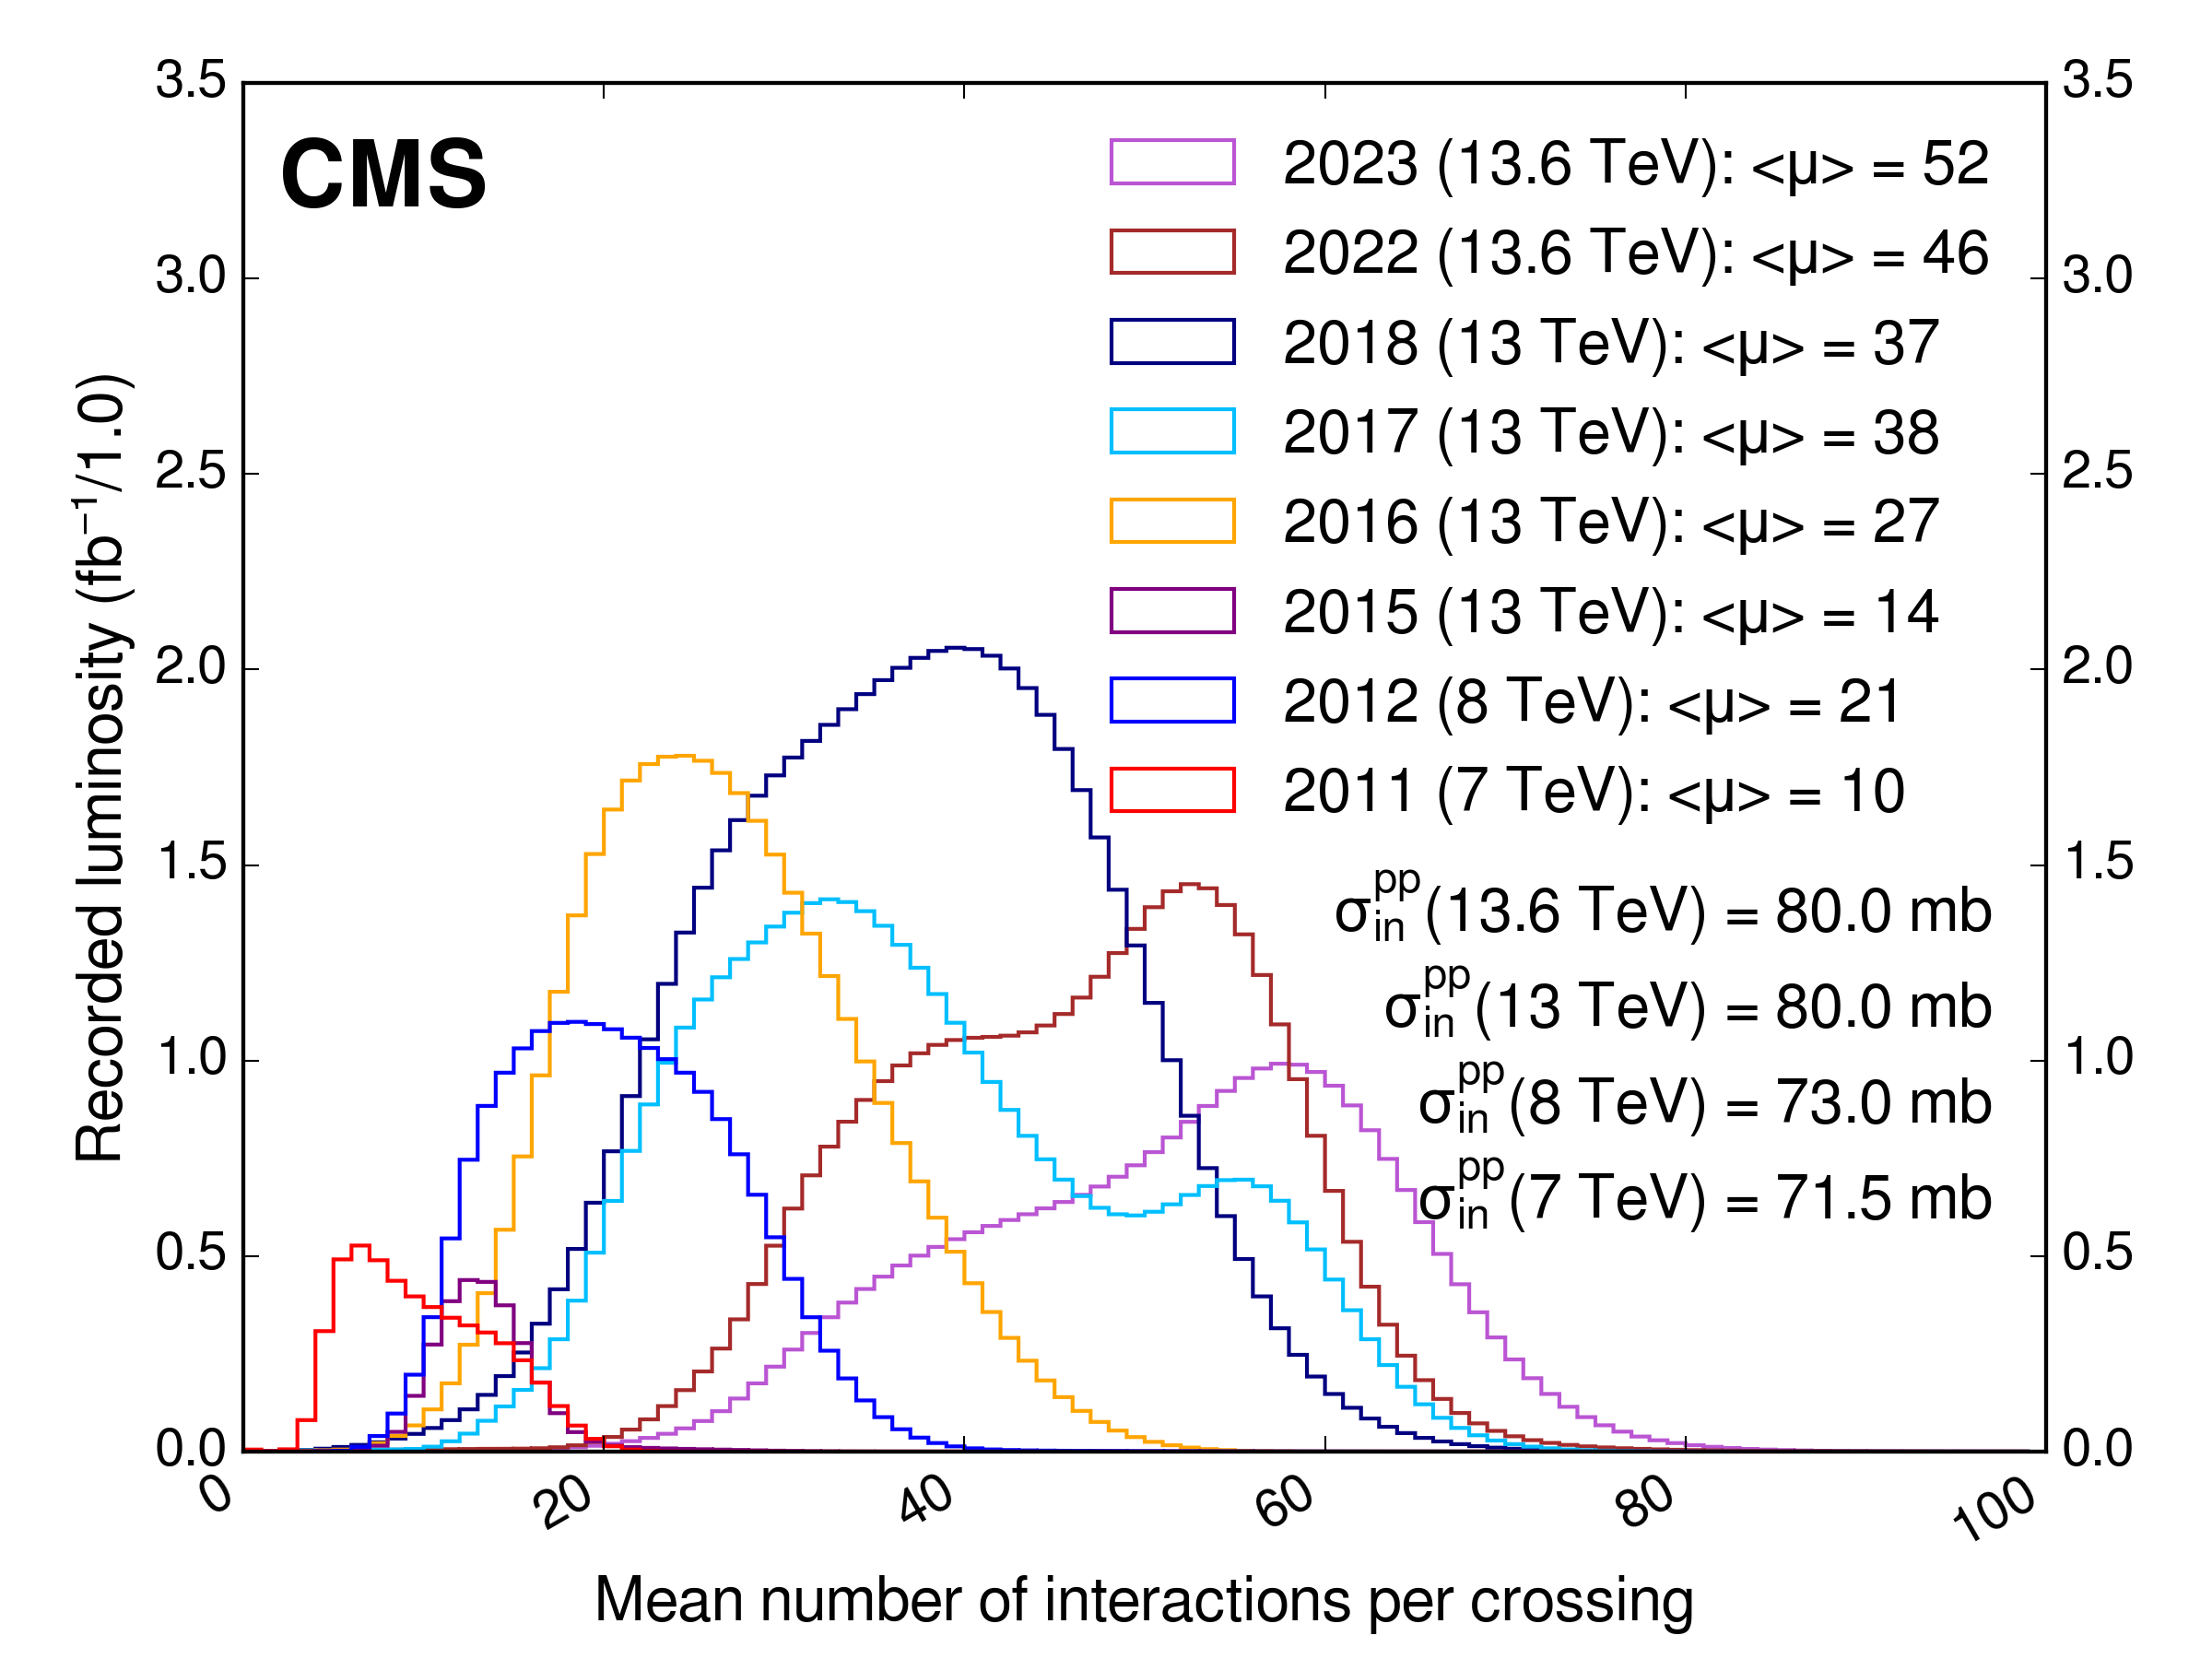
\includegraphics[width=\linewidth]{fig//chap03-cms/pileup.png}
        (b)
    \end{minipage}
    \caption{(a) cumulative integrated luminosity delivered and recorded by the CMS experiment; (b) PU distribution across different years at the CMS experiment \cite{LumiPublicResultsTWiki}}
    \label{fig:lumi_pu}
\end{figure}
\paragraph*{Physics runs}
The LHC program covers a period of $\sim$ 30 years, divided into two phases. 
The \emph{Phase I} includes Run I (2011-2012), Run II (2015-2018), and Run III (2022-2025).
During Phase I the center of mass energy was increased from $7 \TeV$ to $13.6 \TeV$ and the instantaneous luminosity reached a peak of $\mathcal{L}= 2.1 \cdot 10^{34}cm^{-2} s^{-1}$. \\
At the end of 2025, the LHC will enter the \emph{High Luminosity} LHC (HL-LHC) phase, a new phase of upgrades that will take the center of mass energy to 14 \TeV and to an instantaneous luminosity of $\mathcal{L}=5 \cdot 10^{34}cm^{-2} s^{-1}$, providing an integrated luminosity during all the Phase II (2029-2040) of $\mathcal{L}_I=3000 fb^{-1}$, ten times more than in Phase I.\\
During the long shutdown 3 (LS3: 2025-2029) the detectors will be upgraded, along the LHC, to be able to work in such a challenging environment that causes more radiation damage, especially in the forward subdetectors, and with a significant PU increase. up to <PU>$\sim 200$ \cite{Aberle2020SubmitterReport}. 

\iffalse
\begin{figure}[h!]
    \centering
    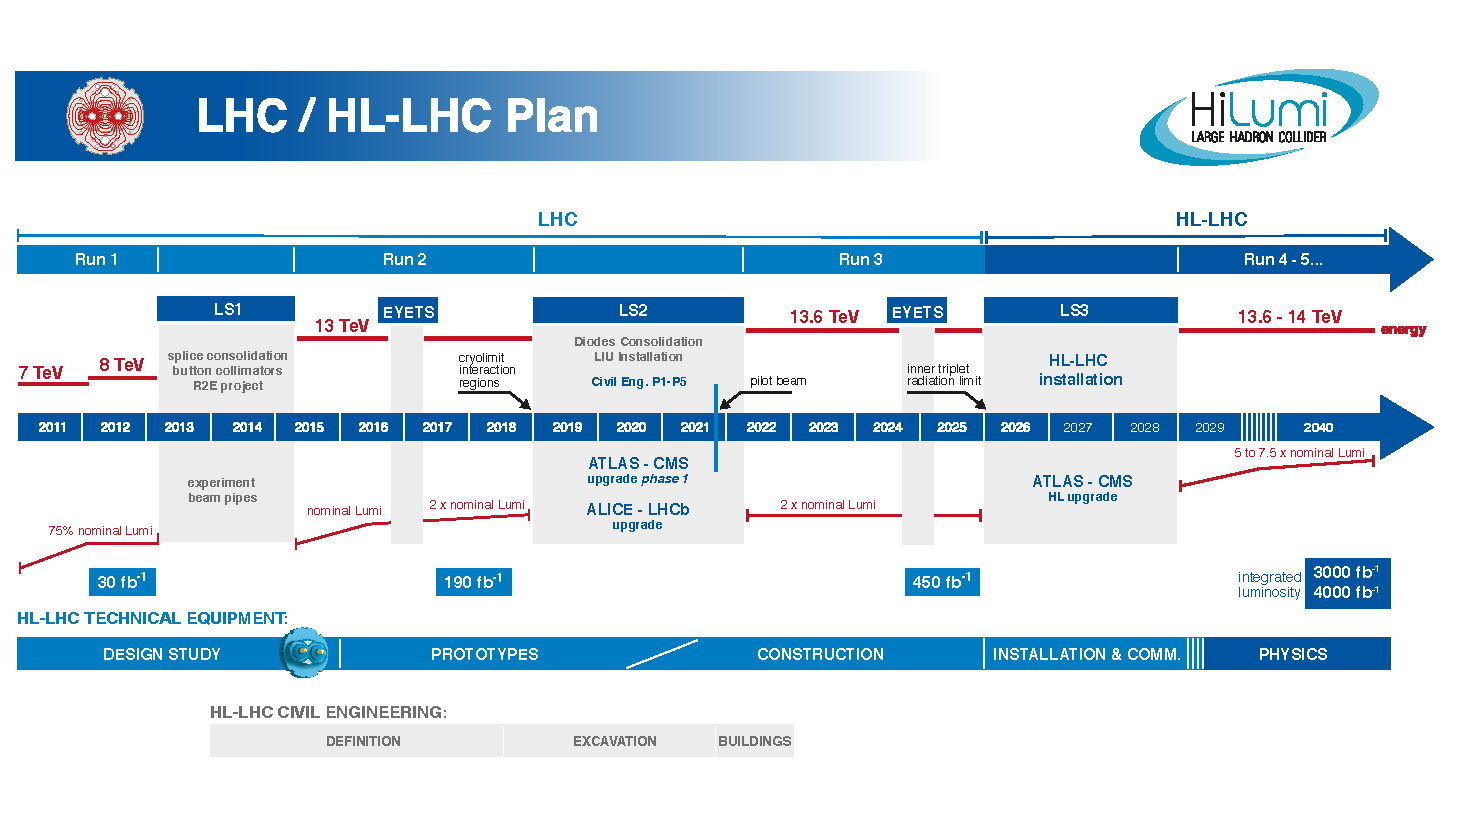
\includegraphics[width=1\linewidth]{fig//chap03-cms/LHC_schedule.pdf}
    \caption{Schedule of the LHC operations \cite{LS3Project}}
    \label{fig:lhc_schedule}
\end{figure}
\fi

\section{The Compact Muon Solenoid experiment}
The CMS experiment \cite{Chatrchyan2008TheLHC} is one of the two largest general-purpose detectors operating at CERN, located in Cessy(FR), 100 m underground at the LHC Point 5 (P5).\\
It is a cylindrical detector, 21.6 m long with a diameter of 14.6 m and a weight of 12500 tons, with coverage in pseudorapidity up to $|\eta|<3.0$\footnote{$\eta=-ln(\tan (\theta/2))$ where $\theta$ is the azimuthal angle in spherical coordinates} extended up to $|\eta|<5.0$ by the high forward Cherenkov calorimeter.\\
It consists of several subdetector layers, as shown in \Fig{fig:cms_exploded}: from inside out, the silicon tracker, the electromagnetic calorimeter (ECAL) and the hadronic calorimeter (HCAL) contained inside the solenoid magnet and the muon system embedded in the flux-return yoke outside the magnet.\\
The key features of the CMS detector are the strong solenoidal magnetic field of 3.8T that is designed to optimize the $p_T$ resolution of charged particles and a PbWO4 electromagnetic calorimeter that improves the $e/\gamma$ identification and resolution to maximize the sensitivity to the low mass $\gamma \gamma$ resonances.\\
These choices have some drawbacks: the PbWO4 crystals suffer radiation damage, becoming more and more opaque in time, and the solenoidal magnet constraint the size of the hadronic calorimeter to just 7 nuclear interaction lengths\footnote{The nuclear interaction length $\lambda$ of a certain material is the mean distance that hadronic particles travel in the material before interacting with a nucleus \label{fn:ncl}}, in contrast to the $10\lambda$ of the ATLAS experiment, affecting the jet energy resolution \cite{Spiropulu2012LHCsDETECTORS}.
\begin{figure}[h!]
    \centering
    \includegraphics[width=1\linewidth]{fig//chap03-cms/CMS_detector_white.pdf}
    \caption{Exploded view of the CMS detector \cite{Chatrchyan2008TheLHC}}
    \label{fig:cms_exploded}
\end{figure}

\subsection{Magnet}
The solenoid magnet \cite{Coroller1997TheReport} is the core element of the CMS experiment that has constrained the design of the rest of the detector.\\
The purpose of the magnet is to bend the tracks of charged particles, due to the Lorentz force, and allow us to measure the transverse momentum $p_T$ of the particle. The stronger the magnetic field, the better will be the $p_T$ resolution.\\
The magnet's coil is made up of multiple layers of superconducting niobium-titanium (NbTi) wires wound together that are cooled using liquid helium down to 4.7 K, allowing the coil to work in the superconductive regime.\\
The solenoidal geometry generates a quasi-uniform magnetic field inside the volume of the magnet of 3.8 T.
The solenoid is surrounded by the steel \emph{return yoke}, composed of five three-layered dodecagonal barrel wheels and three endcap disks at each end.  The yoke contributes to only 8\% of the central magnetic flux density \cite{Chatrchyan2010PreciseRays}. Its main role is to increase the field homogeneity inside the solenoid, closing the magnetic circuit and preventing magnetic leakage. It also hosts the muon system, embedding it in a 2 T magnetic field.

\begin{minipage}{\linewidth} 
    \vspace{0.5cm}
    %\hspace{-0.65cm}
    \begin{minipage}{0.65\linewidth}
        \centering
        \includegraphics[width=1\linewidth]{fig//chap03-cms/magnetic_field.png}
        \captionof{figure}{Field lines and magnitude of the magnetic field of the CMS solenoid magnet \cite{Chatrchyan2010PreciseRays}.}
        \label{fig:magnetic_field}
    \end{minipage}
    \hfill
    \begin{minipage}{0.3\linewidth}
        \centering
        \begin{tabular}{l|c}
            \hline
            Length &  12.5 m\\
            Diameter & 6 m\\
            Weight &  220 tons\\
            Solenoid $|B|$ &  3.8 T\\
            Yoke $|B|$ & 2 T\\
            \hline
        \end{tabular}
        \vspace{0.4cm}
        \captionof{table}{Specifics of the magnet}
    \end{minipage}
\end{minipage}

\subsection{Tracker}
The silicon tracker \cite{CastaldiPatriceSiegristJean-EudesAugustin1997TheReport,CMS_pixel_Phase1_2012} is the closest subdetector to the IP, covering the region $|\eta|<2.5$, and allows us to reconstruct the tracks of charged particles and their transverse momentum, measuring the curvature of the track caused by the magnet.
\begin{figure}[h!]
    \centering
    \includegraphics[width=0.73\linewidth]{fig//chap03-cms/CMS_tracker_Phase1_edit.pdf}
    \caption{Schematic view of a quarter of the CMS tracker in the $r-a$ plane. Pixel modules are shown in green, single-sided strip modules in red and double-sided strip modules in blue \cite{DPGResultsTRKTWiki}.}
    \label{fig:cms_tracker}
\end{figure}
\\
All the modules that compose the tracker are silicon semiconductor sensors and are divided into pixel modules that contain about 66 million pixel cells each with a size of $100 \times 150 \mu m^2$, and strips modules that contain strips of thickness from $80 \mu m$ to $205 \mu m$ and a length that increases with the pseudorapidity.\\
\\
The \emph{pixel tracker} \cite{Adam2021TheUpgrade} is the nearest component to the beam pipe. Its scope is not only limited to collecting the particle hits to reconstruct the tracks, but also to identifying and reconstructing the primary and secondary vertices. The vertex reconstruction is crucial to mitigate PU effects and to identify the decay of displaced particles, enhancing the b-tagging capabilities.
The high granularity of the pixel modules allows achieving these goals. Furthermore, being closest to the IP, the inner tracker has to be designed to be more radiation tolerant than the outer tracker.\\
The pixel tracker is composed of different parts:
\begin{itemize}
    \item \textbf{Barrel pixel (BPIX)}: 4 concentric layers of pixel modules.
    \item \textbf{Forward pixel (FPIX)}: 6 disks of pixel modules
    \begin{table}[h!]
        \centering
        \begin{tabular}{l|c|c|c|c}
            & Radius & z position & Number of & Dose \\
            & [mm]   &  [mm]    &  pixel modules & [Mrad]\\
            \hline
            BPIX & \multicolumn{4}{c}{ } \\
            \hline
            L1&29&-270 to +270&96& 100 \\
            L2&68&-270 to +270&224& 47\\
            L3&109&-270 to +270&352& 22\\
            L4&160&-270 to +270&512& 13 \\
            \hline
            FPIX & \multicolumn{4}{c}{ } \\
            \hline
            D1 inner&45–110&±338&88 & 21-106\\
            D1 outer&96–161&±309&136 & 13-28\\
            D2 inner&45–110&±413&88 & 21-106\\
            D2 outer&96–161&±384&136 & 13-28\\
            D3 inner&45–110&±508&88 & 21-106\\
            D3 outer&96–161&±479&136 & 13-28\\
        \end{tabular}
        \caption{Summary of average r, z positions, number of modules and dose for the four BPIX layers and
the six FPIX rings \cite{Adam2021TheUpgrade}.}
        \label{tab:pixel_tracker}
    \end{table}
\end{itemize}
The \emph{strip tracker} \cite{Friedl2001TheReadout} is composed of  $\sim 20000$ strip modules. Depending on the positions, the geometry of the sensors and the number of strips vary: In the barrel region, the sensors are rectangular, while the endcap sensors are trapezoidal.\\
Some modules are double-sided (DS) strip modules, \ie two single-sided (SS) strip modules mounted back to back with a strip inclination of 5.7° against each other (stereo configuration) to resolve the ambiguity on the z coordinate.


\begin{itemize}

    \item \textbf{Tracker inner barrel (TIB)}: 2 layers of DS + 2 layers of SS strip modules 
    \item \textbf{Tracker inner disk (TID)}: 2 layers of DS + 1 layers of SS strip modules 
    \item \textbf{Tracker outer barrel (TOB)}: 2 layers of DS + 4 layers of SS strip modules 
    \item \textbf{Tracker endcap (TEC)}: 3 layers of DS + 4 layers of SS strip modules 
\end{itemize}
\begin{table}[h!]
    \centering
    \fontsize{11.5pt}{11.5pt}\selectfont
    \begin{tabular}{l|c|c|c|c|c}
        Layer&Radius[mm]&Type&Modules&Pitch[mm]&Strips\\
        \hline
        TIB1&250&DS&336&80&768\\
        TIB2& 340& DS& 456& 80& 768\\
        TIB3&430&SS&552&120&512\\
        TIB4&520&SS&648&120&512\\
        TOB5&610&DS&504&122/183&768/512\\
        TOB6&696&DS&576&122/183&768/512\\
        TOB7&782&SS&648&183&512\\
        TOB8&868&SS&720&183&512\\
        TOB9&965&SS&792&122&768\\
        TOB10&1080&SS&888&122&768\\
        TID1&277&DS&144&81-112&768\\
        TID2&367&DS&144&113-143&768\\
        TID3&447&SS&240&124-158&512\\
        TEC1&277&DS&144&81-112&768\\
        TEC2&367&DS&288&113-143&768\\
        TEC3&447&SS&640&124-158&512\\
        TEC4&562&SS&1008&113-139&512\\
        TEC5&677&DS&720&126-156&768\\
        TEC6&891&SS&1008&163-205&512\\
        TEC7&991&SS&1440&140-172&512\\
    \end{tabular}
    \caption{Summary of average r, type, number of modules, pitch, and number of strips for the strip tracker \cite{Friedl2001TheReadout}.}
    \label{tab:strip_tracker}
\end{table}
The design of the tracker has to consider the multiple scattering, bremsstrahlung and photon conversion that can occur in the tracker itself and that can alter the trajectory and the measurement of the energy deposited in the calorimeter. This implies that the tracker should minimize the material budget without sacrificing the tracking capabilities.


\stepcounter{myfootnote}
\begin{figure}[H]
\centering
\begin{minipage}{\linewidth}
    \centering
\begin{minipage}{0.43\linewidth}
        \centering
        \includegraphics[width=\linewidth]{fig/chap03-cms/material_budget_lambda.png}
\end{minipage}
\hfill
\begin{minipage}{0.43\linewidth}
        \centering
        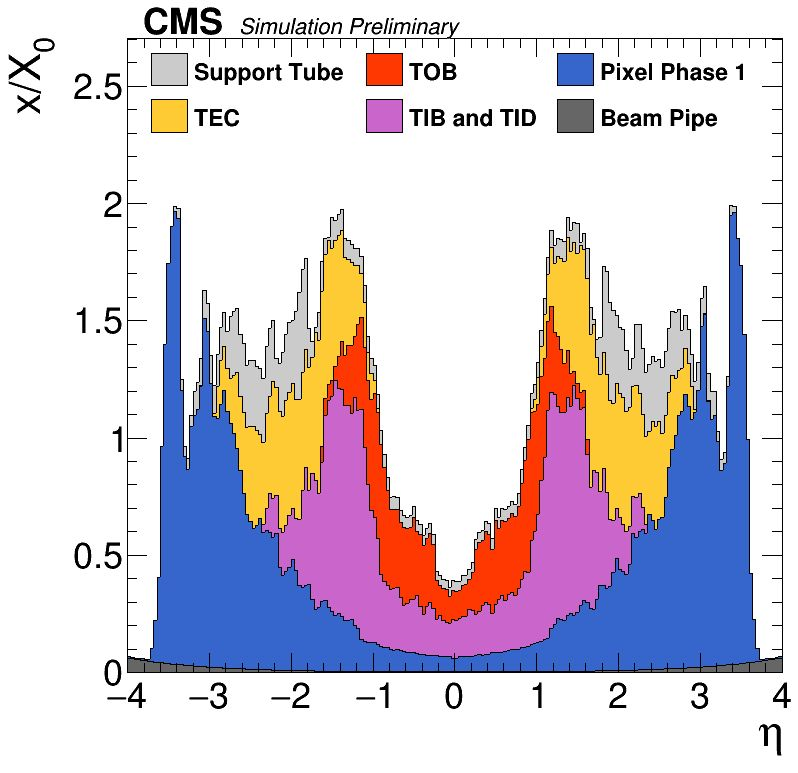
\includegraphics[width=\linewidth]{fig/chap03-cms/material_budget_X.png}
\end{minipage}
\caption[AAA]{Stacked histogram of the thickness of the subparts of the tracker traversed by a particle originated in the IP in function of $\eta$ ((left) in nuclear interaction length units\footnotemark, (right) in radiation length units)  \cite{TrackerMaterialBudgetplotsTWiki}.}
\end{minipage}
\end{figure}

%Footnote of the figure above
\footnotetext{The radiation length $X_0$ of a given material is the length for which, for an electromagnetic particle that travels into the material, holds $E(z)=E_0 e^{-z/X_0}$ where $E(z)$ is the energy of the particle that is a function of the length traveled into the material and $E_0$ the initial energy.}


\subsection{Electromagnetic calorimeter}
The CMS electromagnetic calorimeter (ECAL) \cite{HoferETHZurichHansHofer1997TheReport,Biino2015TheProjections} is the subdetector dedicated to the identification and measurement of the energy of particles that interact primarily via the electromagnetic interaction.\\
One of the main goals of the CMS collaboration was the Higgs boson discovery and, to maximize the discovery sensitivity on the channel $H \to \gamma \gamma$, the ECAL should have met some requirements as high granularity and hermeticity, fast response ($\sim 25ns$), particle identification/isolation/energy at trigger level and linear response in a large energy range (5\GeV to 5\TeV).\\


To comply with these requirements, the ECAL was built using PbWO4 crystals: a high-density material ($\delta=8.28g/cm^3$) with a short radiation length ($X_0=0.85cm$) and a small Moliere radius\footnote{The Moliere radius $R_M$ is the mean radius of the cylinder that contains 90\% of the shower, which tends to disperse due to multiple scattering} ($R_M=2.19cm$).\\
The crystals emit optical light by scintillation in a short time (80\% of the light in 25ns, which is the time separation between two different bunch crossing) but, the light yields of only $\sim 100 \gamma/\MeV$ force the usage of an active photodetector and, due to the presence of the magnetic field, the silicon photomultipliers (SiPM) were the most logical choice.
The ECAL is made of a barrel that covers the $|\eta|<1.479$ region and two endcaps that cover the region $1.479<|\eta|<3.0$.

\begin{figure}[h!]
    \centering
    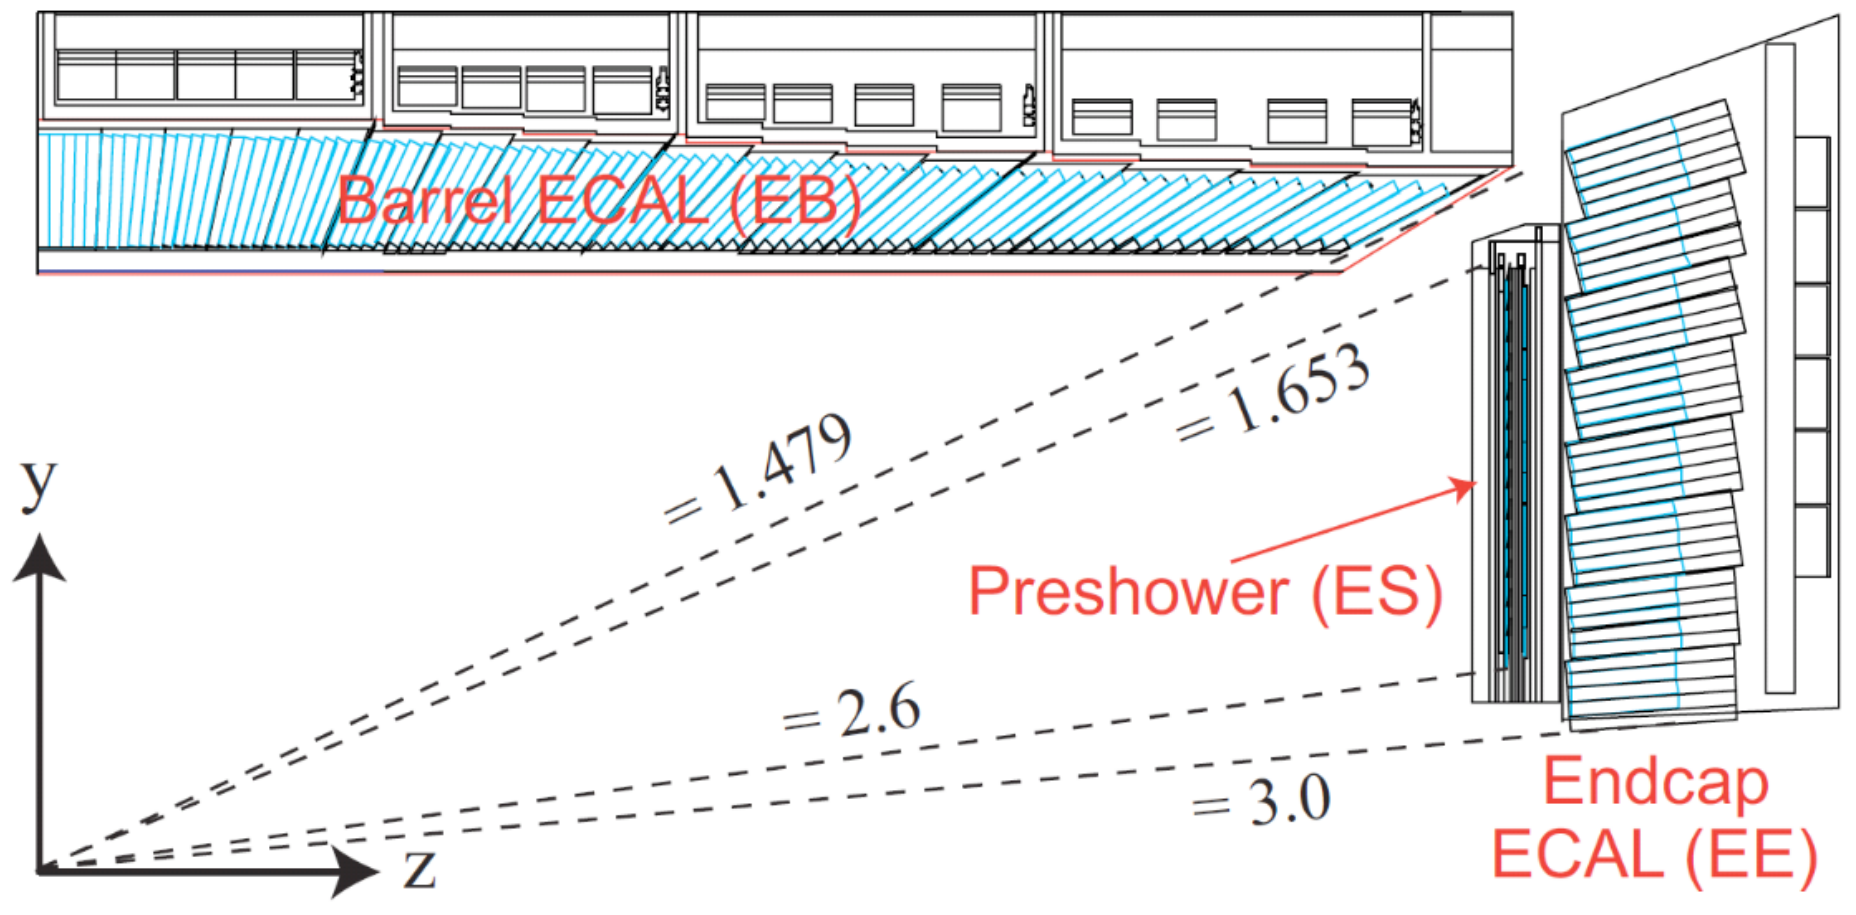
\includegraphics[width=0.7\linewidth]{fig/chap03-cms/ecal.png}
    \caption{Schematic view in the r-z plane of a quarter of the CMS ECAL \cite{Benaglia2014TheExamples}.}
    \label{fig:ecal}
\end{figure}
The ECAL endcaps are composed of 14648 crystals of size $3\times3\times22 cm^3 (\sim25X_0)$ and the ECAL barrel is composed of 61200 crystals of size $2.2\times2.2\times23 cm^3 (\sim26X_0)$. The crystals are not aligned to the IP to avoid cracks aligned with particle trajectories.\\
Furthermore, a pre-shower silicon detector made of 4288 strip modules is placed in front of the endcaps to improve the $\gamma-\pi^0$ separation\footnote{The $\pi^0$ decay $\pi^0 \to \gamma \gamma$ can cause the misidentification of a pion into a photon.}.
\\
\\
The energy resolution of the PbWO4 crystals measured with an electron beam without magnetic field and radiation damage was \cite{Adzic2007EnergyCalorimeter} 
\begin{equation}
    {\frac{\sigma_{E}}{E}}={\frac{2.8\%}{\sqrt{E[{\mathrm{GeV}}]}}}\oplus{\frac{0.127 \GeV}{E[{\mathrm{GeV}}]}}\oplus0.3\%
\end{equation}
where the first term is the stochastic term, the second is the noise term and the third is the constant term that contains the calibration errors and the leakage of the energy.\\
In the CMS detector, the ECAL energy resolution is worse mainly due to the presence of the tracker between the ECAL and the IP and due to the transparency variations induced by radiation damage and the aging of photomultipliers, but, during the Run1, the ECAL was able to achieve the $\sim1\%$ energy resolution for high-energy electrons \cite{Chatrchyan2013EnergyTeV}.\\
The radiation damage of PbWO4 crystals is constantly monitored by a laser system in various $\eta$ intervals as shown in \Fig{fig:ecal_rad_damage}.
\begin{figure}[h!]
    \centering
    \includegraphics[width=0.85\linewidth]{fig//chap03-cms/rad_damage.png}
    \caption{ECAL relative response to the laser monitoring system from 2011 to 2019 \cite{EcalDPGResultsCMSDPS2019005TWiki}.}
    \label{fig:ecal_rad_damage}
\end{figure}

\subsection{Hadronic calorimeter}
Hadrons usually don't deposit all their energy in the ECAL, especially neutral hadrons, therefore the ECAL is surrounded by the hadronic calorimeter HCAL that allows the measurements of the jets' energy and the missing energy.\\
The CMS HCAL \cite{Green1997TheReport,Anderson2012CMSCalorimeter} is divided into four subdetectors: the hadron barrel (HB), the hadron endcaps (HE), the hadron outer (HO), and the hadron forward (HF).\\
The HB is a sampling calorimeter made of brass absorbers and plastic scintillators that act as active material. The brass was chosen due to its short interaction length and because it is non-magnetic.\\
It covers the pseudorapidity region $|\eta|<1.3$ and it extends in a radius $1.77m<R<2.95m$. The barrel is divided into sections of size $(\Delta \eta, \Delta \phi)=0.087 \times 0.087$ and is composed of eight 50.5 mm thick and six 56.5 mm thick brass plates alternating with the scintillating tiles, that are connected through optical cables to SiPM sensors to collect and amplify the light.\\
The total thickness of the HB in nuclear interaction length units at $|\eta|=0$ is $5.82 \lambda_I$ that increases up to $10.6\lambda_I$ at $|\eta|=1.3$.\\
In addition to this, the ECAL barrel adds $\sim 1.1\lambda_I$ thickness of material.\\
\begin{figure}[h!]
    \centering
    \includegraphics[width=0.85\linewidth]{fig//chap03-cms/hcal.png}
    \caption{Schematic view in the r-z plane of a quarter of the CMS HCAL and depth segmentation after the Phase I update \cite{Anderson2012CMSCalorimeter}. }
    \label{fig:hcal}
\end{figure}
\\
Also the HE is a sampling calorimeter made of brass absorbers and plastic scintillating tiles. It is divided into 18 sectors in $\phi$ and into 14 sectors in $\eta$ (the size increases with $\eta$) and is placed 4006.5 mm from the interaction point. It covers the $1.3 < |\eta|<3.0$ region and including the ECAL endcaps, its length in interaction lengths units is $\sim10\lambda_I$\\
\\
The HO is placed outside the solenoid magnet, and its purpose is to catch the tails of the hadronic showers that are not contained by the HB. The HO is composed by five scintillator rings with a radius of 4.07 m that cover the region $|\eta|<1.26$. The central ring that covers the thinner HCAL region is equipped also with a 19.5 cm thick iron absorber and an additional scintillator, as shown in fig \Fig{fig:ecal_rad_damage}.\\
\\
The HF is a sampling calorimeter is located 11150 mm away from the interaction point and covers the region $3<|\eta|<5.2$. It is composed of 1.65 mm steel absorber plates and 0.6 mm thick quartz fibers that emit light by Cherenkov effect. It is also used for the online monitoring of luminosity.
\\
The combined energy resolution of the ECAL and the HCAL was measured using a pion beam from 2 \GeV to 350 \GeV \cite{Abdullin2008TheGeV/c}
\begin{equation}
    \frac{\sigma_E}{E}= \frac{84.7\%}{\sqrt{E}} \oplus 7.4 \%
\end{equation}
The energy resolution is mainly affected by the sampling fluctuations and the noise term is negligible.

\subsection{Muon system}
The CMS muon system \cite{Layter1997TheReport} is embedded in the iron return yoke and its scope is to collect muon hits that are used, in combination with information from the tracker, to enhance the identification of muons and momentum resolution of high-energy muons.
It is divided into five separate wheels in the barrel, containing four layers of detectors, and four independent endcaps for each side.

\begin{figure}[h!]
    \centering
    \includegraphics[width=0.85\linewidth]{fig//chap03-cms/muon_system.jpg}
    \caption{Schematic view in the $r-z$ plane of a quarter of the muon system \cite{Piccolo2011CMSPerformance}.}
    \label{fig:muon_system}
\end{figure}


Three different gaseous detector technologies are employed:
\begin{itemize}
    \item \textbf{Drift tubes chambers (DT)}: The 250 DT chambers are divided into five wheels and cover the region $|\eta|<1.2$. Each wheel is divided into 12 sectors covering $\Delta \phi=30º$ around the interaction point, and each sector is organized into four muon barrels (MB).
    Each chamber consists of 8 or 12 aluminum layers with up to 90 tubes.

    \item \textbf{Cathode strip chambers (CSC)}: CSCs consist of arrays of anode wires crossed with copper cathode strips within a gas volume. The 486 CSCs are organized in 4 layers, placed in the endcap disks, and extend the muon system coverage up to $0.8<|\eta|<2.4$

    
    \item \textbf{Resistive plate chambers (RPC)}: The RPCs are located both in the barrel and in the endcap region, up to $|\eta|<1.6$. RPCs consist of two charged parallel high resistive plastic plates filled with gas. The read-out is performed by aluminum strips separated from the graphite coating. The scope of the RPCs is to provide, in combination with the DTs and the CSCs, a fast signal to exploit for the muon trigger system.
\end{itemize}

\begin{figure}[H]
    \centering
    \begin{subfigure}[b]{.58\linewidth}
        
        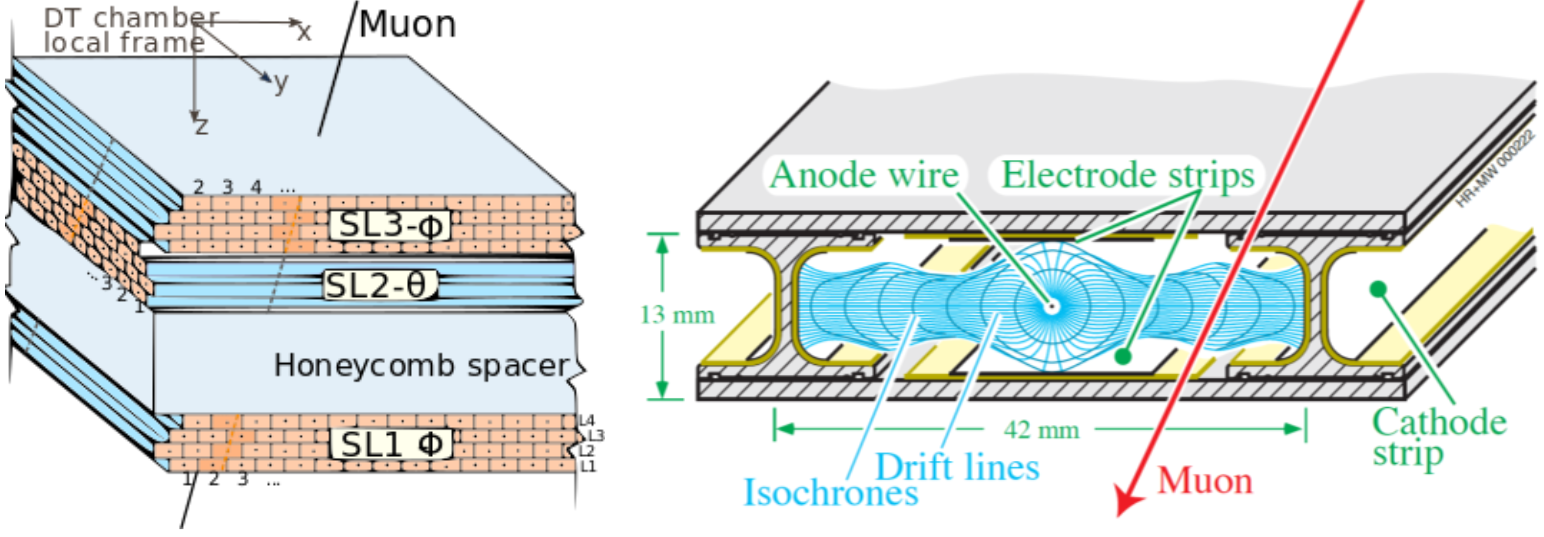
\includegraphics[width=\linewidth]{fig//chap03-cms/drift_tubes.png}
        \label{fig:drift_tubes}
        \caption{}
    \end{subfigure}
    \begin{subfigure}[b]{.41\linewidth}
        
        \includegraphics[width=1\linewidth]{fig//chap03-cms/rpc.png}
        \caption{}
        \label{fig:rpc}
    \end{subfigure}
    \begin{subfigure}[b]{0.7\linewidth}
        \centering
        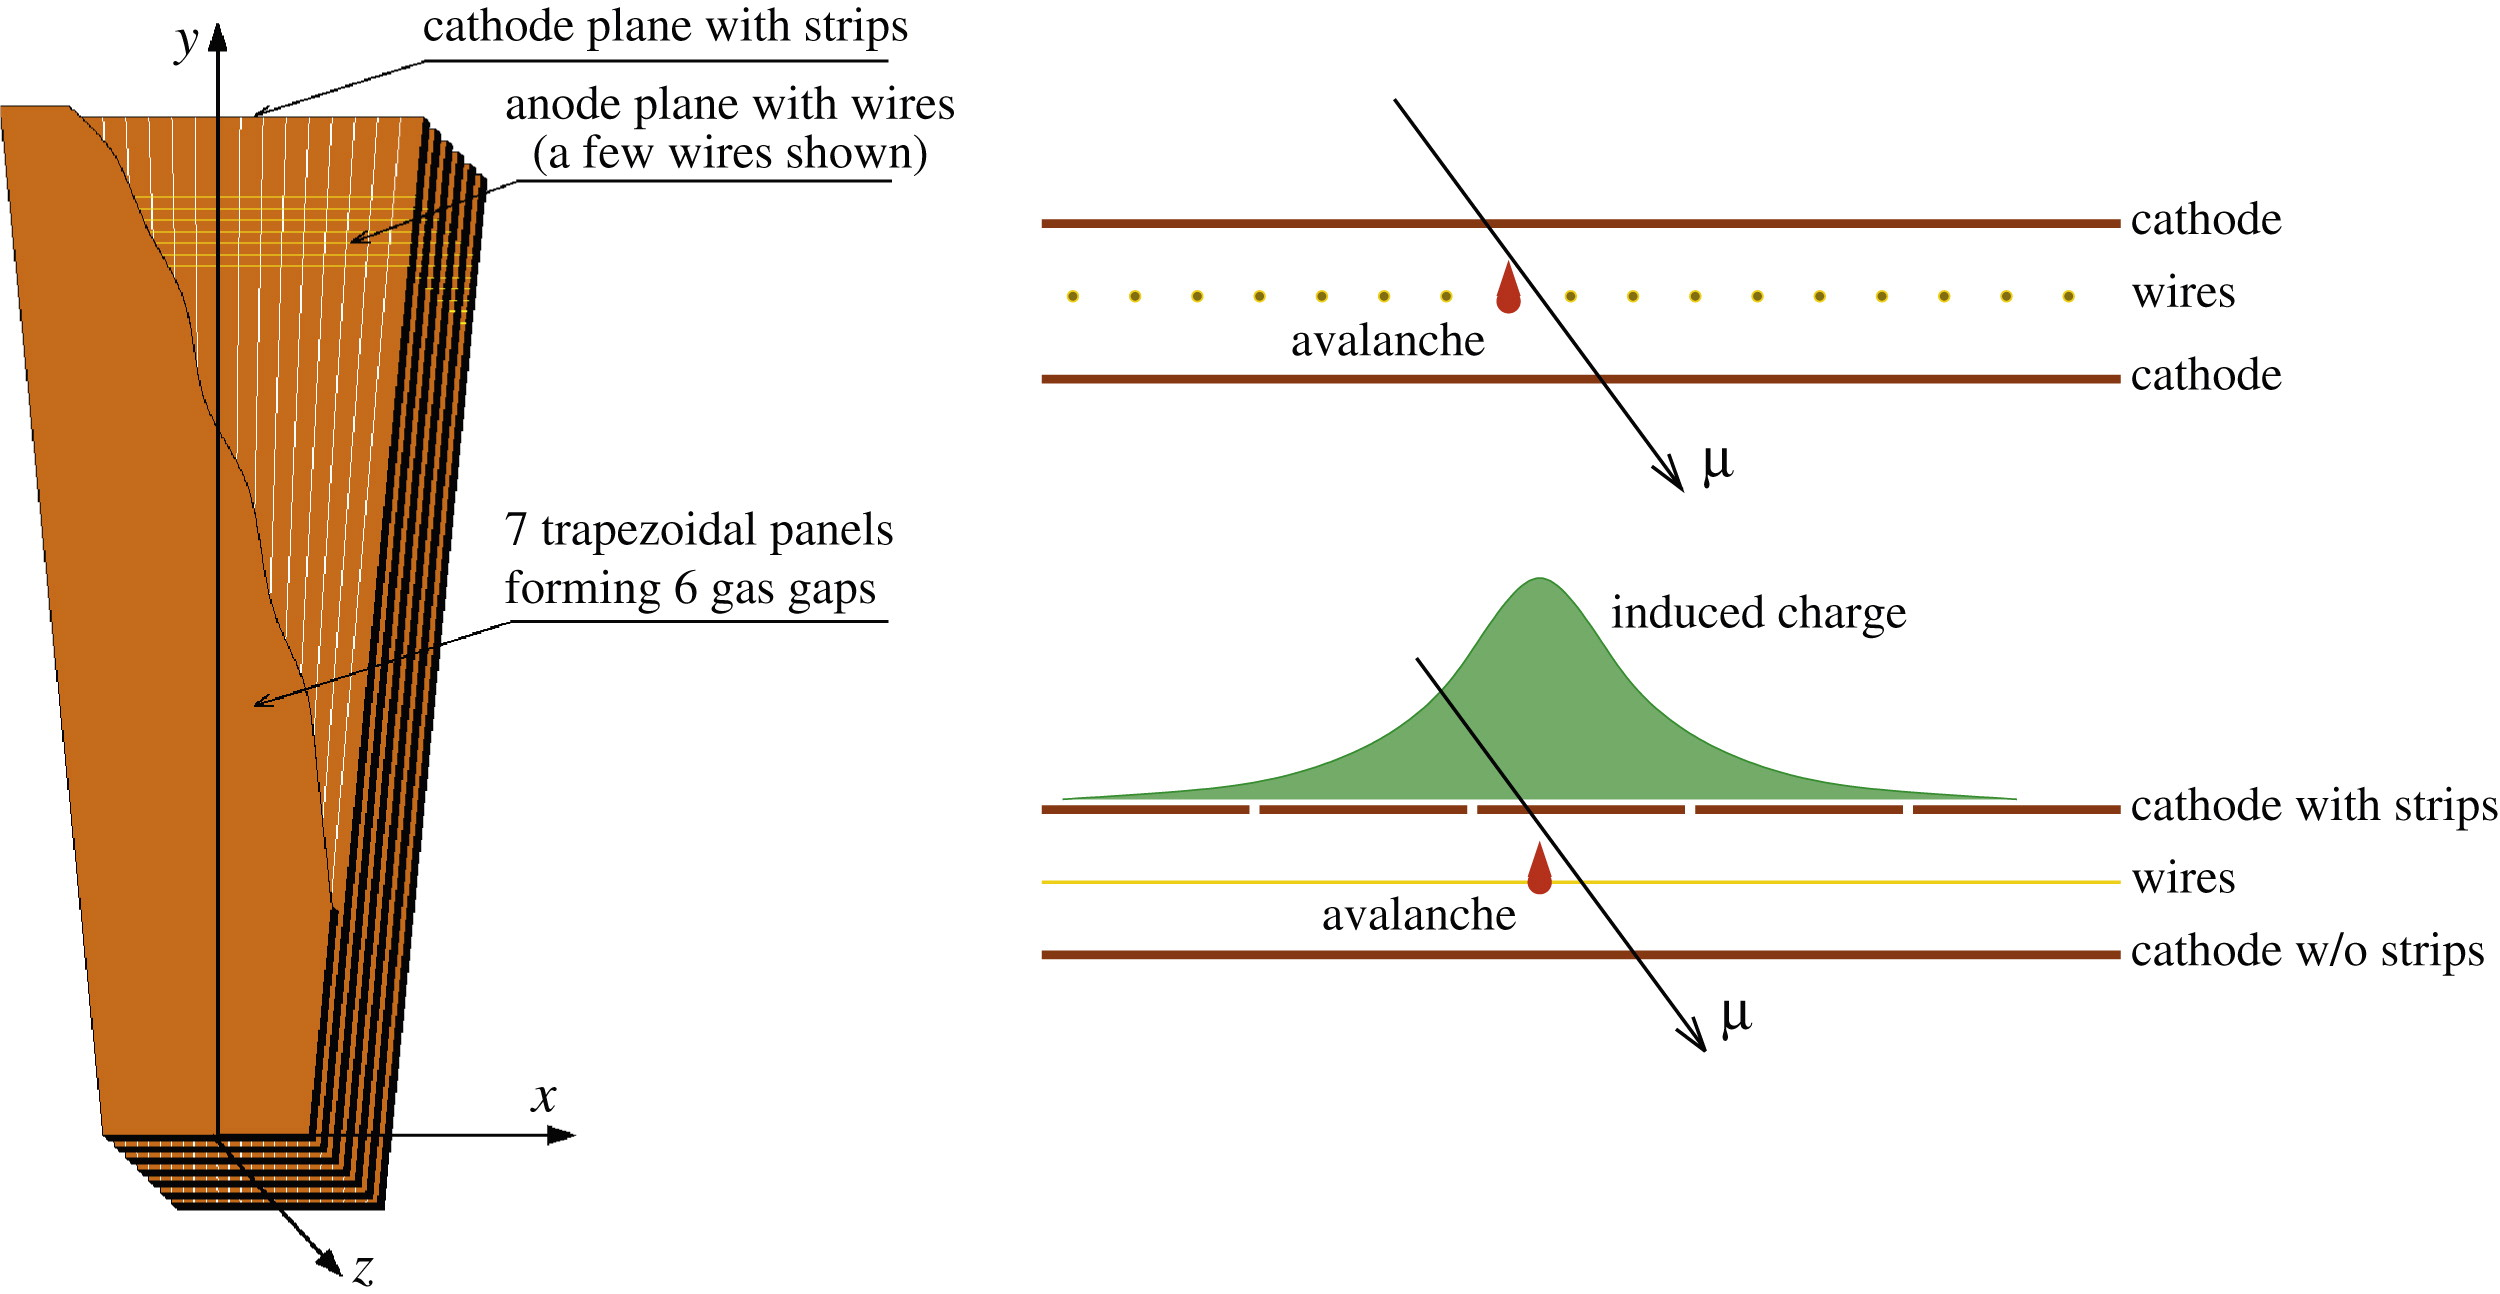
\includegraphics[width=1\linewidth]{fig//chap03-cms/csc.jpg}
        \caption{}
        \label{fig:csc}
    \end{subfigure}
    \caption{Schematics view of the (a) drift tubes chamber \cite{MuonExperiment}, (b) resistive plates \cite{EndcapReshufflingRpcTWiki}, (c) cathode strips chamber \cite{Acosta2008EfficiencyChambers}.}
    \label{fig:muons_technologies}
\end{figure}
    


\subsection{Trigger and data acquisition}
At LHC, bunch crossing occurs each 25ns. Considering the raw event size of 1 MB \cite{Franzoni2016DatasetAnalyses}, this would lead to a data throughput of  $\sim 1$ TB/s at the nominal luminosity, that, not only will saturate the bandwidth of the data acquisition system but also would make it impossible to save on tape all the recorded data.\\
The scope of the CMS trigger system is to select only the events relevant to the CMS physics program.
The trigger system is divided into the level 1 low-level trigger (L1) and the high-level trigger.\\
\\
The CMS L1 Trigger \cite{Musenich2000CMSSystems} operates as a hardware-based trigger system exploiting FPGA boards. It relies on custom algorithms that have to make decisions within $3.2 \mu s$, the maximum time that the raw data can occupy the buffers.\\
The L1 trigger collects raw data from the front-end electronics of the calorimeters and the muon system that converts the analog signals to digital.\\
The algorithms roughly estimate the energy deposit and the trajectory of the particles in the subdetectors to select EM, jet, and muon candidates. Thereafter, the information from the muon system and from the calorimeters are combined into the global trigger that chooses whether to discard the event or to pass it to the HLT trigger for further filtering.
The L1 trigger reduces the output rate from the bunch crossing rate of $40$MHz to $100$kHz.
\\
\begin{figure}[h!]
    \centering
    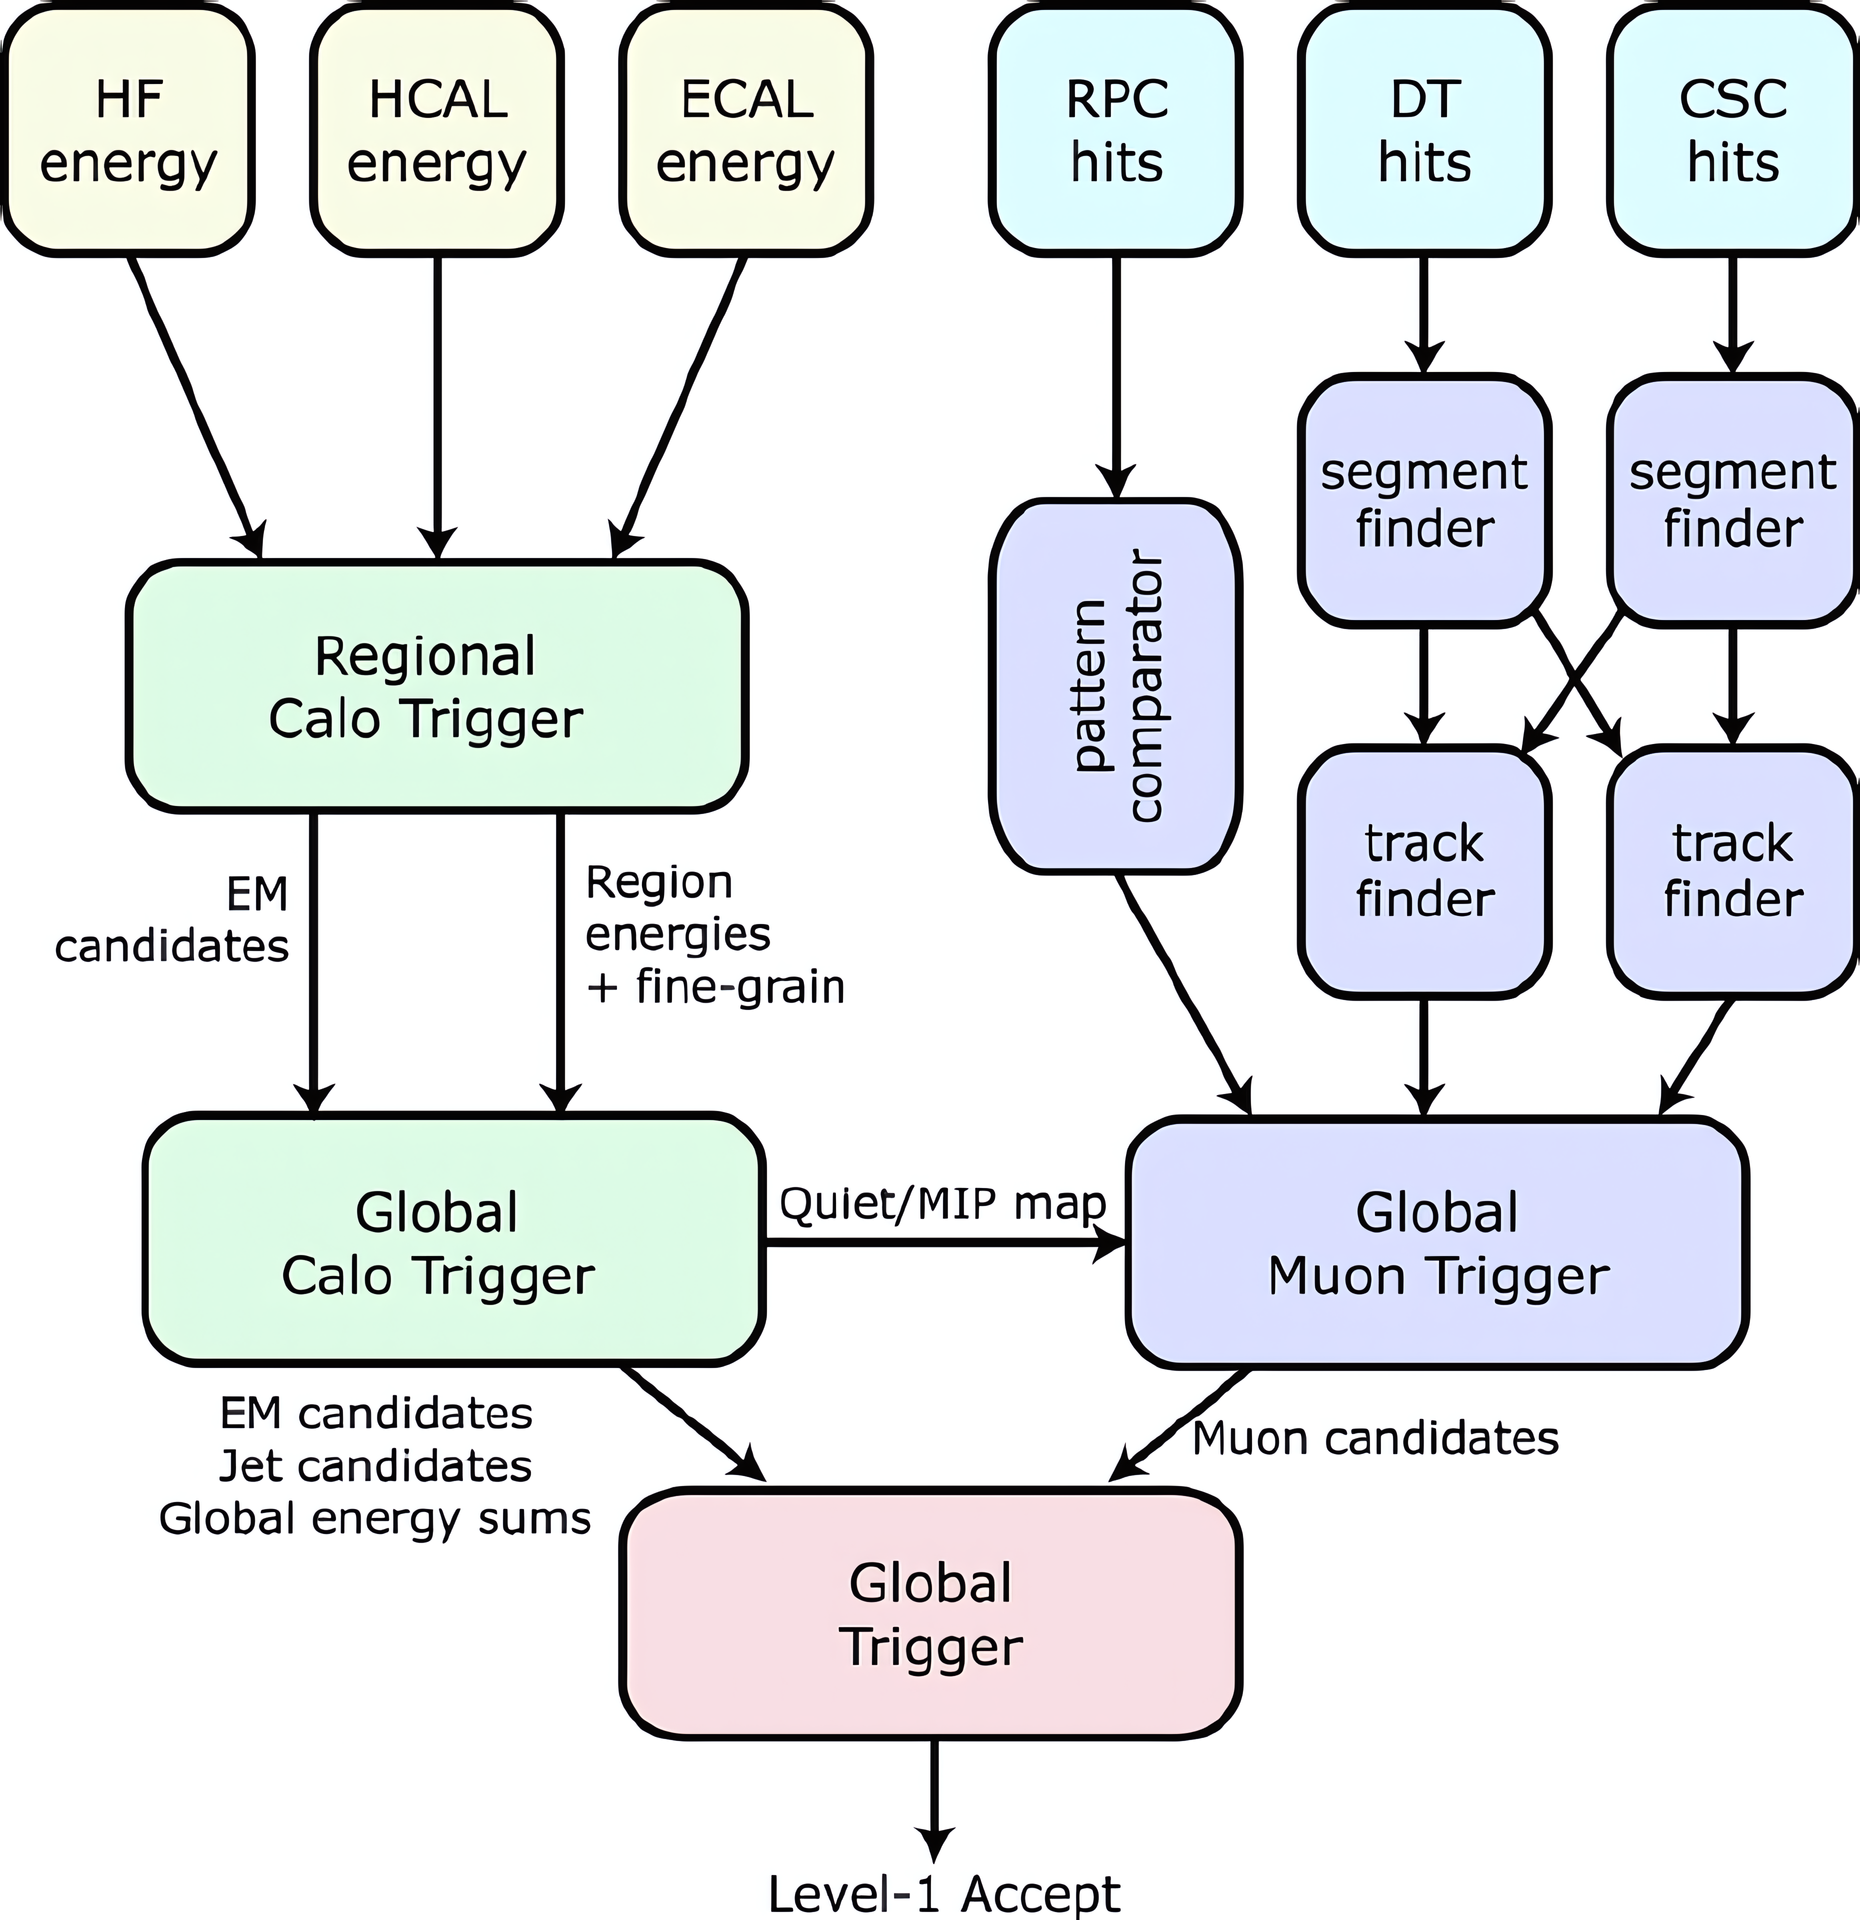
\includegraphics[width=0.6\linewidth]{fig/chap03-cms/L1_upscayl_2x_remacri_upscayl_2x_remacri.png}
    \caption{Architecture of the Level-1 Trigger \cite{Brooke2003HardwareTrigger}.}
    \label{fig:l1}
\end{figure}
\\
The HLT system \cite{Racz2002CMSTrigger} is a software-based trigger implemented on a computer farm composed of 16000 CPUs that decreases the output rate from the 100 kHz of the L1 trigger to 1 kHz. It employs the same algorithms used by the offline reconstruction but adapted to the timing constraint of the HLT trigger.
It has access to the full detector readout, and events are accepted or rejected as soon as there is enough information to decide. The raw data of the events that are accepted by the trigger are saved on tape and the events are reconstructed offline when the computing resources are available.


%%!TEX root = ../thesis.tex

\newchap{Event simulation and reconstruction}\label{sec:RECO}
\vspace{-1cm}
\minitoc

\section{Event reconstruction}\label{sec:PF}
The event reconstruction is the identification of all the particles and their kinematics from each pp collision, starting from the raw data that is just a collection of hits and energy clusters.\\
CMS is a highly segmented detector, designed to give a different signature for each kind of particle.
All the charged particles produce tracks, electrons, and photons produce a shower in the ECAL, hadrons start showering in the ECAL and are absorbed in the HCAL, while muons, due to their mass, are minimum ionizing particles that penetrate all the detector, leaving tracks in the tracker and the muon system (\Fig{fig:PF}).
\begin{figure}[h!]
    \centering
    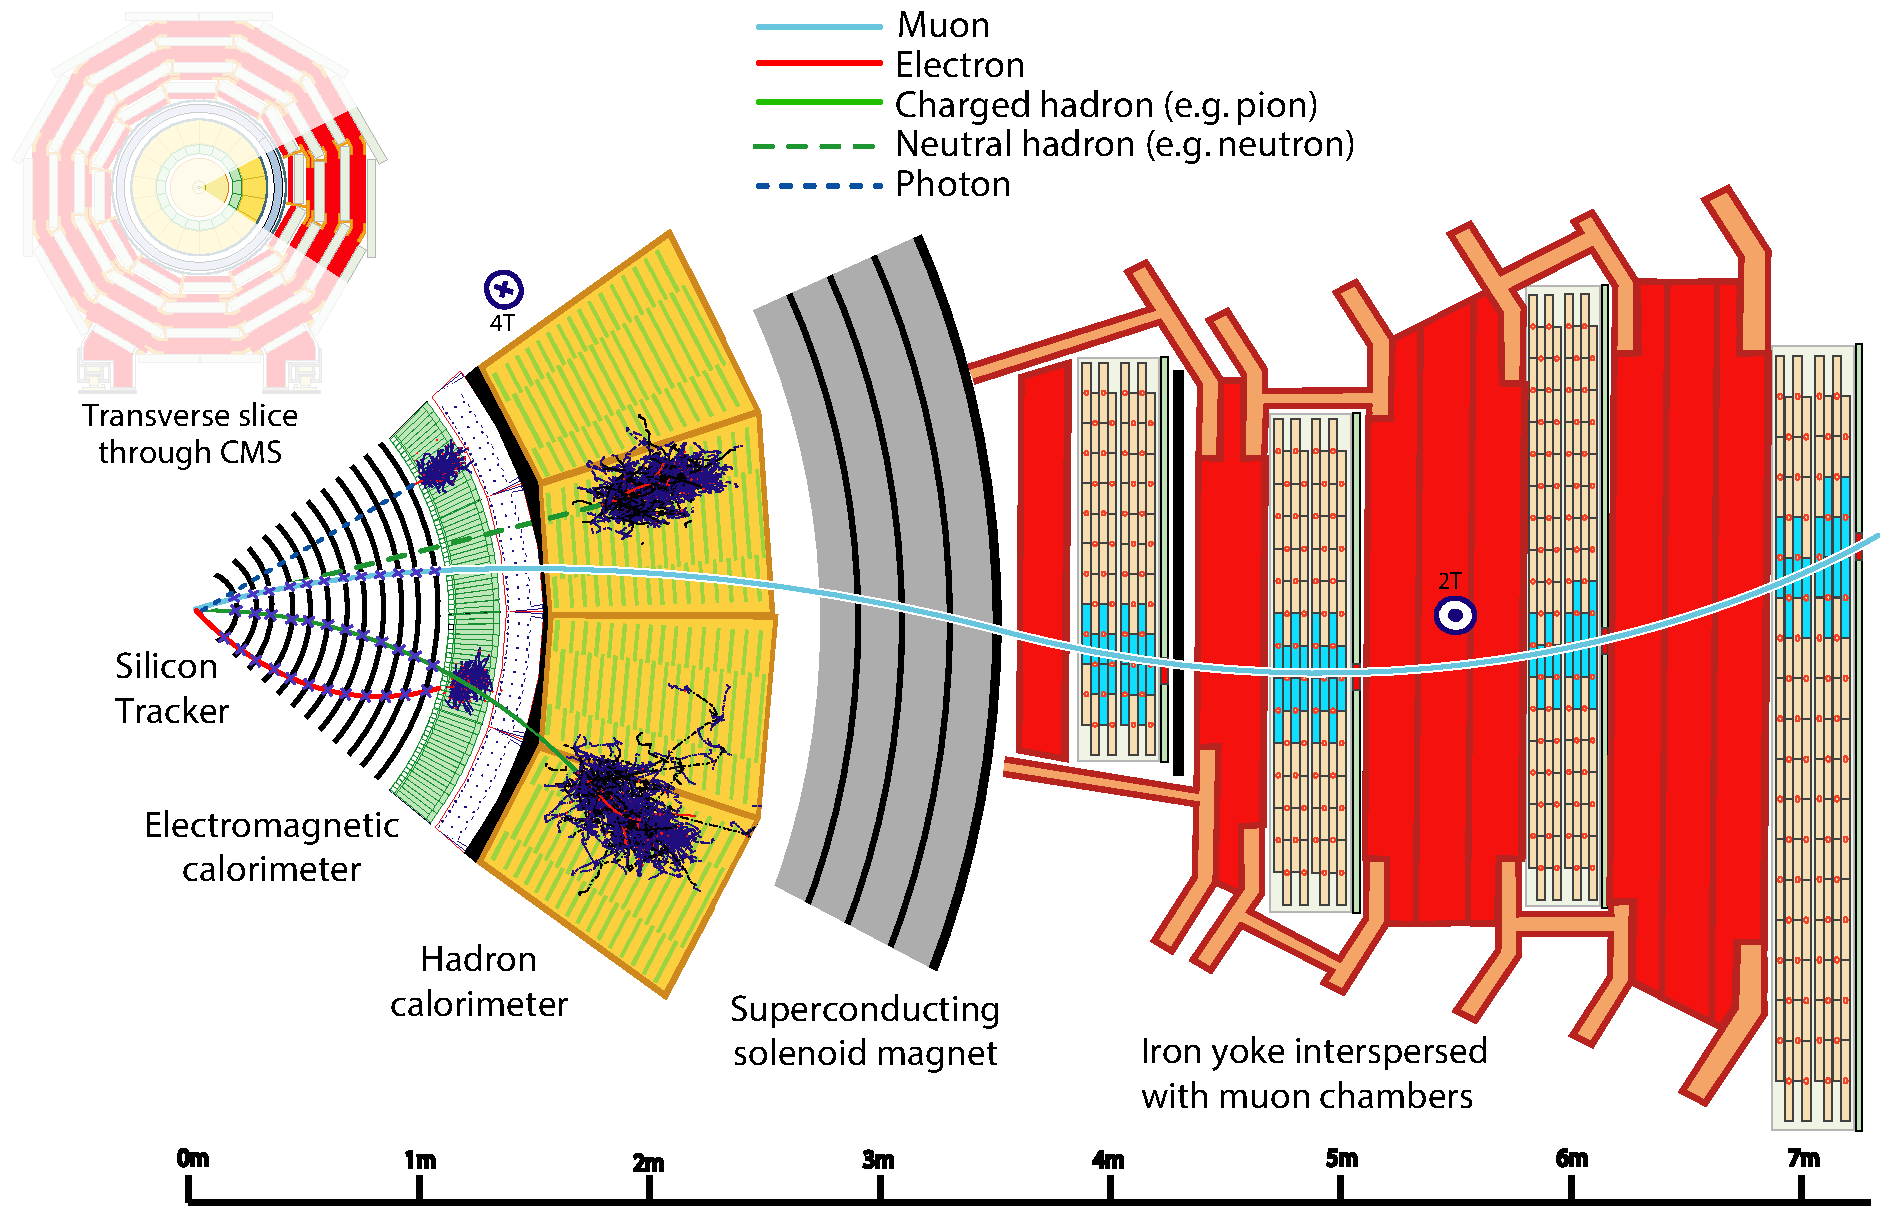
\includegraphics[width=\linewidth]{fig//chap04-reco/CMS_detector_PID_edit.pdf}
    \caption{Signatures of different types of particles in a slice of the CMS detector. The muon and the charged pion are positively charged, and the electron is negatively charged. \cite{Sirunyan2017Particle-flowDetector}}
    \label{fig:PF}
\end{figure}
\\
The informations of the different subdetectors are linked together to improve the resolution of the detector and to consider other signatures (\eg reconstructing a photon that has converted an electron-positron pair in the tracker).
This approach is called Particle Flow (PF) \cite{Sirunyan2017Particle-flowDetector}, and each reconstructed particle is called a PF candidate.



\subsection{Tracking}\label{sec:tracking}
The algorithm used to reconstruct the trajectories of charged particles and their momentum is the Combinatorial Track Finder (CTF) \cite{Chatrchyan2014DescriptionTracker}, an adaptation of the Kalman Filtering (KF) \cite{Fruhwirth1987ApplicationFitting} algorithm.
At the beginning, a few hits in consecutive layers of the tracker are used as seed of the KF algorithms and then a final fit is performed to estimate the position of the vertex, the direction, and the momentum of each charged particle.\\

\paragraph*{Seeding and iterations}
This process is iterated in multiple steps, starting with searching for tracks that are easier to find (\eg particle with large $p_T$ produced in the IP), removing the associated hits to reduce the combinatorial multiplicity, and searching for other kinds of tracks using different seeding criteria (Table \ref{tab:track_seeding}).

\begin{table}[h!]
    \centering
    \begin{tabular}{|c|c|c|c|}
    \hline
    Iteration&Name&Seeding&Targeted Tracks\\
    \hline
    1& InitialStep&pixel triplets&prompt, high $p_T$\\
    2& DetachedTriplet&pixel triplets&from b hadron decays, $R\leq 5$cm\\
    3& LowPtTriplet&pixel triplets&prompt, low $p_T$\\
    4& PixelPair&pixel pairs&recover high $p_T$\\
    5& MixedTriplet&pixel+strip&triplets displaced, $R\leq 7$cm\\
    6& PixelLess&strip triplets/pairs&very displaced, $R\leq 25$cm\\
    7& TobTec&strip triplets/pairs&very displaced, $R\leq 60$cm\\
    8& JetCoreRegional&pixel+strip pairs&inside high $p_T$ jets\\
    9& MuonSeededInOut&muon-tagged&tracks muons\\
    10& MuonSeededOutIn&muon detectors&muons \\
    \hline
    \end{tabular}
    \caption{Seeding configuration of ten iterations with different target tracks. $R$ is the target distance of the track origin from the beam axis \cite{Sirunyan2017Particle-flowDetector}. }
    \label{tab:track_seeding}
\end{table}

\paragraph*{Track finding}
The track finding is divided into four steps:
\begin{enumerate}
    \item Using the parameter of the track candidate (given by the seed at the beginning), determine which successive layer of the tracker can be intersected by the trajectory, considering its uncertainties.\\ The trajectories are assumed to be perfect Helix, neglecting the multiple scattering, allowing us to use fast analytical methods.
    \item Look for a compatible silicon module\footnote{Silicon modules usually overlap, so in this step the algorithms look for groups of modules, also to ease the computational effort.} in the layer such that its boundary is less than $3 \sigma$ from the trajectory. The trajectory and its uncertainties are propagated to the sensor surface.
    \item A $\chi^2$ test is used to check which of the hits are compatible with the track candidate, considering both the hit and the trajectory uncertainties.
    \item Update the track candidate and iterate
\end{enumerate}
\paragraph*{Track fitting}
To determine the track parameters, after all hits of each track are assigned by the track finder, a new KF fit is initialized at the location of the innermost hit. The fit proceeds through all the hits, from inside outwards.\\
This filter is followed by a smoothing stage that consists of a second KF initialized with the result of the first one and is run backward. The track parameters are obtained from a weighted average of the track parameters of these two filters.\\
During the track fitting stage, the effects of interaction with materials and  inhomogeneous of the magnetic field are considered.

\begin{figure}[H]
    \centering
    \includegraphics[width=0.75\linewidth]{fig//chap04-reco/KF.png}
    \caption{Visualization of the forward filter and the backward smoother filter. The red points indicate the measurements and their uncertainties on each layer, while the green points indicate the predictions \cite{Ai2021AFitting}.}
    \label{fig:KF}
\end{figure}

\subsubsection*{Muon tracks}
The reconstruction of muon tracks combines the information from the tracker and the muon system. Three types of tracks are defined:
\begin{itemize}
    \item \textbf{Standalone muons}: Tracks built using only the hits in the muon system.
    \item \textbf{Tracker muons}: Tracks built using only the hits in the tracker that match the track segments in the muon system.
    \item \textbf{Global muons}: Tracks fitted combining the tracker and the muon system hits, improving the $p_T$ resolution of the tracking detector.
\end{itemize}
Usually, there is no reason to not use global muons, but low $p_T$ muons can be reconstructed as tracker muons because of the large multiple scattering in the return yoke. 

\subsubsection*{Electron tracks}
The initial identification of electrons is performed in two ways:
The first consists of estimating the electron momentum from the $\phi$ spreading of the ECAL cluster and finding a track compatible with the cluster.
The second method consists of finding ECAL clusters compatible with tracks extrapolated  from the tracker.\\
\\
Electrons, traversing the tracker, radiate energy by Bremsstrahlung. For this reason, the KF doesn't perform well, so, tracks that are identified as electrons are refitted with the Gaussian sum filter (GSF) algorithm \cite{Adam2003ReconstructionLHC} that approximates the energy loss of electrons, described by the Bethe-Heitler distribution \cite{Bethe1934OnElectrons}, as a Gaussian mixture.\\
At each layer, a set of helical track segments is computed for a different value of the energy loss, and it's weighted with the corresponding probability of occurring. These informations are used to decrease the energy of the particle and update the trajectory uncertainties at each layer.
\subsubsection*{Vertex reconstruction}
Once all the tracks are reconstructed, those that come from the same vertex are clustered together and a fit is performed to determine the vertex position.\\
The fit is done using the simulated annealing algorithm \cite{Kirkpatrick1983OptimizationAnnealing} that estimates the vertex position by minimizing a free energy function and associates to each track the probability of belonging to the i-th vertex. \\

\subsection{Calorimeter clustering}
The clustering in calorimeters is necessary to reconstruct photons (in the ECAL) and neutral hadrons (in the HCAL), objects that don't leave any signature in the tracker system.\\
The ECAL is also used to improve the identification of electrons, matching the tracks with the ECAL energy clusters and looking for bremsstrahlung photons, and both the ECAL and the HCAL to improve the reconstruction of charged hadrons, especially the high energetic ones.\\
Cluster seeds are built from cells with an energy larger than a given threshold and
larger than the energy of the neighboring cells.\\
Starting from the seeds, topological clusters are built by aggregating neighboring cells that have an energy larger than twice the noise level.\\
Assuming that the energy deposit in the M cells contained in the topological cluster arises from N Gaussian energy deposits, one for each seed in the topological cluster, a Gaussian mixture model is used to reconstruct the cluster. The parameters of the Gaussian are the location parameters in the $(\eta,\phi)$ plane and the amplitude, while the width has a fixed value, different for each subdetector.\\
The energy and the position of the seeds are used as initial values for the parameters of the Gaussian mixture that are estimated through an analytical maximum likelihood fit.\\

\begin{table}[h!]
    \centering
    \begin{tabular}{|c|cc|cc|c|}
    \hline
    &\multicolumn{2}{c|}{ECAL} & \multicolumn{2}{c|}{HCAL} & Preshower\\
    &barrel&endcaps&barrel&endcaps& \\
    \hline
    Cell E threshold (MeV)&80&300&800&800&0.06\\
    Seed \# closest cells&8&8&4&4&8\\
    Seed E threshold (MeV)&230&600&800&1100&0.12\\
    Seed ET threshold (MeV)&0&150&0&0&0\\
    Gaussian width (cm)&1.5&1.5&10.0&10.0&0.2\\
    \hline
    \end{tabular}
    \caption{Seeding and clustering parameters for the ECAL, the HCAL, and the pre-showers \cite{Sirunyan2017Particle-flowDetector}.}
    \label{tab:clustering}
\end{table}

\subsection{ParticleFlow linking}
The PF elements are initially built separately in each subdetector and each of them can be linked with other PF elements in their k-nearest neighborhood \cite{Dasarathy1991NearestTechniques} (kNN) in the $(\eta,\phi)$ plane.\\
The linking algorithm assigns a distance between each possible pair of elements that quantifies the quality of the link. All elements that are linked together form a PF block.

\paragraph*{Track to track linking}
Charged particles that originate from a common secondary vertex and have an invariant mass greater than 0.2 \GeV are linked together to reconstruct a nuclear interaction or a displaced decay.

\paragraph*{Track-CaloCluster linking}
A track is linked to a calorimeter cluster if the position of the track in the $(\eta,\phi)$ plane ($(x,y)$ for the endcaps), extrapolated from the hit in the outermost layer, is contained in the union of the cluster areas of the ECAL and HCAL. The cluster areas are enlarged to take into account the uncertainties in the position, multiple scattering, and the presence of cracks between cells.\\
The link distance is defined as the distance between the track and the cluster in the $(\eta,\phi)$ plane for the barrel and in the $(x,y)$ plane for the endcaps, keeping only the link with the smallest distance for each element.\\
Furthermore, photons emitted tangent to electron tracks (with $|\Delta \eta| <0.5$) are collected as Bremsstrahlung photons. They have a significant probability of converting into electron-positron pairs, so a dedicated conversion finder algorithm \cite{Sirunyan2021ElectronLHC}, based on the iterative tracker procedure (discussed in sec \ref{sec:tracking}), is used to link $e^+e^-$ tracks to the corresponding photons.\\
In this step, the clusters associated with electrons and Bremsstrahlung photons are clustered into superclusters.



\paragraph*{Cluster to cluster linking}
When the cluster position of the more granular calorimeter is contained in the cluster area of the less granular calorimeter, the link is established.
Also in this case, the distance is defined as the distance of the cluster positions in the $(\eta,\phi)$ plane for the barrel and in the $(x,y)$ plane for the endcaps and just the link with the smallest distance is kept.

\paragraph*{Track-muon linking}
As explained in sec \ref{sec:tracking}, the PF elements in the tracker are linked with the ones in the muon system through spatial matching to allow the global fitting of the muon tracks.



\subsection{ParticleFlow reconstruction}
In each PF block, muon candidates are identified and reconstructed first. The following steps deal with the reconstruction of electrons, photons, and hadrons.
At each step, the PF blocks used to reconstruct the candidate are removed. In particular, the electron reconstruction is performed before the photon reconstruction to remove elements associated with Bremsstrahlung photons.\\
At the end, when all blocks have been processed, the event is revisited in a post-processing step.

\paragraph*{Muons}
To avoid the misidentification of hadrons in muons (that can occur for high-energy hadrons that reach the muon system), isolated global muons are selected by considering all the tracks and energy deposits within $\Delta R<0.3$ from the muon direction, with the constraint that: the scalar sum of the $p_T$ and the $E_T$ of other elements have to be less than the 10\% of the muon $p_t$; there are at least three track segments in the muon system; and the calorimeter deposit match the $p_t$ estimate from the track.\\
Muons originating from the semileptonic decay of hadrons require more stringent criteria.

\paragraph*{Electrons and photons}
Because electrons emit Bremsstrahlung photons and photons convert to electron pairs, the reconstruction of electrons and photons is performed in the same step.\\
For each supercluster, if it matches a GSF track, an electron candidate is built, if not, a photon candidate is built. \\
All the ECAL clusters in the PF block linked to the supercluster, to the electron track, or tracks belonging to a photon conversion are associated with the candidate.\\
Electron candidates must satisfy additional identification constraints on the amount of energy radiated, the distance between the track and the ECAL cluster in the $(\eta,\phi)$ plane, the ratio of the energy released in the ECAL and the HCAL, the number of hits and goodness of fit of the track reconstructed both with the KF and the GSF. The final identification of the electron is performed by a Boosted decision tree (BDT) that is trained on all these inputs.\\
Photons must satisfy isolation criteria that just require the isolation from other tracks and clusters.

\paragraph*{Hadrons}
The remaining PF blocks in the ECAL that are not linked with a track are identified as non-isolated photons originating from $\pi^0$ decays, while the ones in the HCAL as neutral hadrons.\\
The remaining HCAL clusters are linked to tracks and, eventually, to other remaining ECAL clusters to identify charged hadrons.\\
It is relevant to note that, outside the tracker coverage, charged and neutral hadrons cannot be distinguished anymore.

\paragraph*{Missing transverse momentum}
The neutrinos and other hypothetical exotic particles do not interact with the detector material and the only quantity that we can measure is the missing transverse energy\footnote{We can measure only the transverse component because, at a hadron collider, it is impossible to know the initial state due to the composite nature of the protons}.\\
The missing transverse momentum is defined as the opposite vector to the vectorial sum of the transverse momentum of all the particles.

\begin{equation}
    \vec{p_T}^{\text{miss}}=-\sum_i^{N_{\text{part}}} \vec{p_{T,i}}
\end{equation}

\paragraph*{Post-processing}
The misidentification of high $p_T$ particles or the presence of cosmic rays can lead to a large reconstructed missing energy $p_T^{\text{miss}}$.
The post-processing phase consists of selecting high $p_T$ particles, computing the correlation between the $p_T$ of the particle and the reconstructed missing energy, and changing the identification and the reconstruction of the particles if this at least halves the missing energy amplitude.

\subsection{Jets}\label{sec:jets}
To infer the kinematics of the parton produced in the hard-scattering, hadrons that originated from the hadronization of the parton have to be clustered together into jets.
The clustering algorithm for jets must satisfy two requirements:
\begin{itemize}
    \item \textbf{Collinear safety}: Collinear splitting of the momentum of components of the jet must not change the jet.
    \item \textbf{Infrared safety}: Soft emission must not change the jet.
\end{itemize}
The current algorithm used by the CMS collaboration is the anti-$k_T$ algorithm \cite{Cacciari2008TheAlgorithm}.\\
The anti-kt introduces the custom distances $d_{ij}$ between hadronic PF candidates, and $d_{iB}$ between the PF candidate and the beam spot 
\begin{gather}
    d_{i j}=\operatorname*{min}\left(p_{\mathrm{T}i}^{-2},p_{\mathrm{T}j}^{-2}\right)\cdot\frac{\Delta R_{i j}^{2}}{R^2}\\
    d_{iB}=p_{Ti}^{-2}
\end{gather}
R is a parameter that regulates the dimension of the jet cone. In CMS, jets are constructed using R=0.4 (AK4 jets) but, to study boosted objects that cause jets to merge, R=0.8 (AK8 jets a.k.a. fatjets) is another choice.\\
\\
The algorithm performs as follows
\begin{algorithm}
\caption{anti-$k_T$ algorithm}\label{algo:akt}
\begin{algorithmic}[1]
    \State Compute all the $d_{ij}$ and $d_{iB}$
    \While{\# candidates$>0$}
        \State Select the couple of PF candidates with the minimum $d_{ij}$
        \State Sum their Lorentz vector and replace the two PF candidates with this pseudojet.
        \State Recompute $d_{ij}$ and $d_{iB}$
        \If{$d_{ij}<d_{iB} \; \forall \;j$ }
            \State The i-th candidate is defined as a jet and removed.
        \EndIf
    \EndWhile
\end{algorithmic}
\end{algorithm}
\\
This algorithm tends to cluster soft particles with hard ones instead of clustering soft particles with each other and tends to group all the components in cones.\\
The energy scale and resolution of the jet, and consequently also the missing energy, is corrected afterward, analyzing the composition of the jets  \cite{Khachatryan2017JetTeV}.\\
\\
Jet can also contain contributions from pileup interaction that occurred in the current bunch crossing (in-time pileup) or the previous bunch crossing (out-of-time pileup).\\
In-time pileup contributions from charged hadrons, that are over 50\% of the in-time pileup contribution, can be avoided by subtracting the contribution of charged hadrons originating from pileup vertices while out-of-time pileup is determined by fitting the pulse shape of the calorimeters signals and subtracted to the jet energy afterward.\\
The remaining contributions from pileup are parametrized as a function of $p_T, \eta$, and the jet area.

\subsubsection*{Flavour tagging}
To fully characterize the jet, we must understand which is the flavor of the parton that generated the jet.\\
The identification of b (c) jets (b/c tagging) can be performed by studying the b and c hadrons that compose it.\\
Heavy flavor hadrons have a relatively large lifetime that makes them travel the detector for $\sim 0.3-0.5mm$, which allows us to use displaced tracks and secondary vertices as a signature to recognize heavy flavor jets.\\
Despite that, using a single observable to determine the jet flavor is not efficient enough and a multivariate analysis is required.\\
The model used in the Run II analysis by the CMS collaboration is \DeepJet \cite{Bols2020JetDeepJet}, a neural network (see sec \ADDREF) trained using labeled MC samples of AK4 jets of different flavors.\\
\DeepJet uses $\sim 650$ observables as input, divided into global variables that describe the jet kinematics, charged and neutral PF candidates features (the first 25 ordered by the displacement significance), and secondary vertices features (up to 4 secondary vertices sorted by the flight distance significance).\\
\\
The PF candidate features and the secondary vertices features are fed as input to three different convolutional neural networks (CNN) \cite{OShea2015AnNetworks} and, afterward, to three different recurrent neural networks (RNN) composed of LSTM layers \cite{Sherstinsky2018FundamentalsNetwork} that treat the constituents of the jet as a sequence. The three outputs and the global features are then fed to a dense feed-forward neural network that can classify the jet as b-tagged, c-tagged, or gluon/light-tagged, assigning to each class a score.

\begin{figure}[H]
    \centering
    \includegraphics[width=0.75\linewidth]{fig//chap04-reco/deepjet.png}
    \caption{Illustration of the \DeepJet architecture. \cite{Bols2020JetDeepJet}}
    \label{fig:DeepJet}
\end{figure}
\begin{figure}[H]
    \centering
    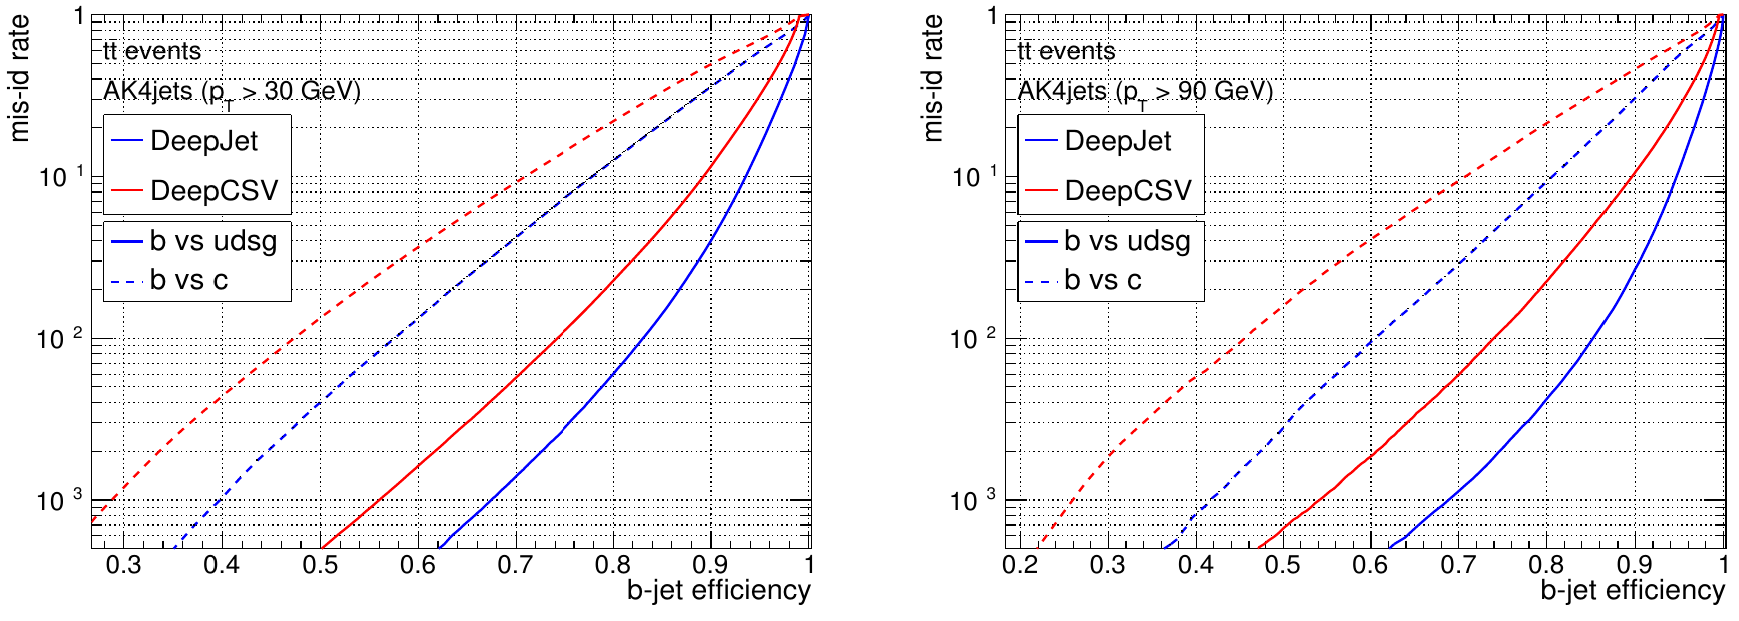
\includegraphics[width=\linewidth]{fig//chap04-reco/bjet.png}
    \caption{Performance comparison between \DeepJet and \DeepCSV, another model based on a simple feed-forward network. \cite{Bols2020JetDeepJet}}
    \label{fig:btag_perform}
\end{figure}



\section{Event simulation}
To optimize the analysis, estimate the efficiencies, evaluate the systematic uncertainties, and interpret the data, we need Monte Carlo simulations (MC): labeled data that reproduces the real data as faithfully as possible.\\
\\
The first stage of the simulation is the generation of the matrix elements, usually done with software like \MADGRAPH \cite{Alwall2011MadGraphBeyond} or \POWHEG \cite{Alioli2010ABOX}: after the user has defined all the Feynman diagrams to compute and the physics model, the four momenta of all the particles are computed at the parton level.
The next step, performed by \PYTHIA \cite{Sjostrand2006PYTHIAManual} in the CMS software, is the hadronization of colored particles, done exploiting the phenomenological Lund string model \cite{Andersson1983PartonDynamics}.\\
\\
The second step, performed by the \GEANTfour framework \cite{Agostinelli2003GEANT4--aToolkit}, is the simulation of the detector response and is the most computationally intensive step, to the point that other approaches to the simulation are being considered \cite{Sekmen2016RecentSimulation,Vaselli2023FlashSimFlow}.\\
\GEANT emulates the propagation of particles through the CMS detector, simulating the particle-matter interactions and the readout of each subdetector. In these steps, the electronic noise, the digitization, the Landau fluctuations, and all the inefficiencies of the detectors like the non-uniformity of the materials are simulated.\\
The events are then reconstructed exactly like the real data, with the same algorithms.\\
Despite the complexity of the full simulation, the MC can't reproduce exactly the real data so, for each analysis, the user has to apply the so-called scale factors (SF) to the MC, a set of event weights that represents the ratios of efficiencies between MC and data $SF=\epsilon_{data}/\epsilon_{MC}$.


%%!TEX root = ../thesis.tex
\newchap{Analysis methods}\label{sec:STAT}
\minitoc
\section{Neural networks}
In this work, neural networks are used as a tool to classify different events in signal or background, giving to the input of the NN different features of the events (like the 4-vectors of all the particles in the event). So, in this section, the discussion will be focused on the classification problem.\\
\\
A neural network (NN) is a machine learning\footnote{Machine learning is the process by which a computer program uses data to infer and build a predictive model.} model that can solve a wide range of problems and make predictions, learning from the data.\\
The learning of an NN can be supervised, if the target of our dataset is known, or, vice versa, unsupervised.\\
In the context of supervised learning, there are mainly two classes of problems that a neural network can address:
\begin{itemize}
    \item \textbf{Regression}: Given a set of inputs $\bm{x} \in \mathbb{R}^N$, predict a set of output $\bm{y} \in \mathbb{R}^M$
    \item \textbf{Classification}: Given a set of inputs $\bm{x} \in \mathbb{R}^N$, predict a set of output $\bm{y} \in \mathbb{Z}_M$
\end{itemize}


\paragraph*{Perceptron}\hspace{1cm}\\
\begin{minipage}{\linewidth}
    \begin{minipage}{0.46\linewidth}
        
    \begin{figure}[H]
        \centering
        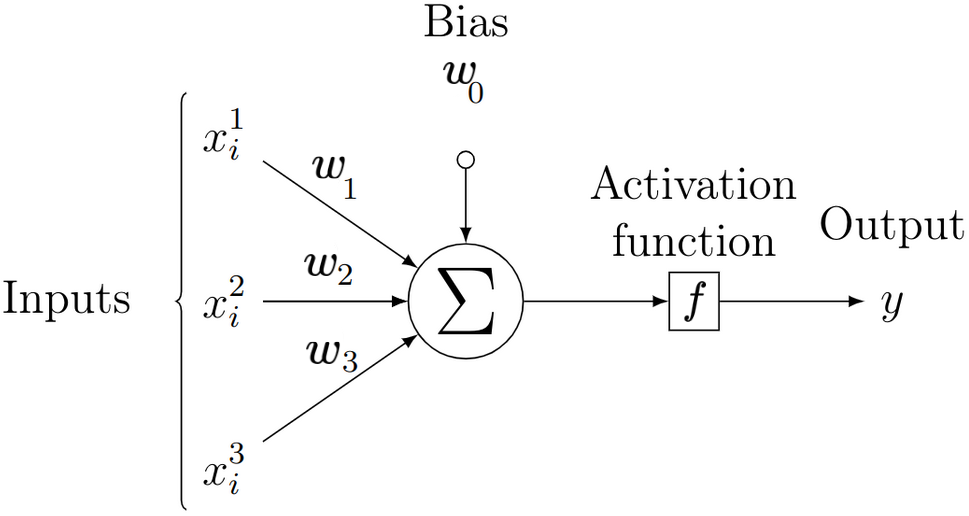
\includegraphics[width=\linewidth]{fig//chap05-stats/perceptron.png}
        \vspace{0.5cm}
        \caption{Visualization of a perceptron with three dimensional inputs $x_{ij}$. Each feature input is multiplied by a weight and everything is summed, along with the bias $w_0$. The result is passed to the activation function $f$, which, in this case, is the Heaviside theta function}
        \label{fig:perceptron}
    \end{figure}
    \end{minipage}
    \hfill
    \begin{minipage}{0.51\linewidth}
    %\vspace{-1.25cm}
        The simplest NN is the Rosenblatt perceptron \cite{Rosenblatt1958TheBrain} (\Fig{fig:perceptron}), a NN with one single neuron that addresses the binary classification problem.\\
        The characteristics of the neuron are:
            \begin{itemize}
                \item The dimension of the input. Each data entry is N-dimensional and each dimension is called a "feature".

                \item Each neuron has N weights, plus one bias, that are tuned through the learning procedure, looking at the data.

                \item The activation function, \ie the function is applied do the dot product $\bm{x}\cdot \bm{w}+w_0$.
                In the case of the perceptron, $f$ is the Heaviside theta function.
            \end{itemize}
    \end{minipage}
    \vspace{0.75cm}
\end{minipage}
\\
Given a set of inputs $\bm{x} \in \mathbb{R}^N$ and a set of weights $\bm{w} \in \mathbb{R}^{N+1}$, the output will be
\begin{equation}
    y=
    \begin{cases}
        1 & \text{if }\sum_{i=1}^N w_i x_i + w_0 >0\\
        0 & \text{Otherwise}
    \end{cases}
\end{equation}
The weights $w_i$ are obtained through the learning procedure.\\
Given $\hat{y}_i$ the truth label of the input $\bm{x}_i$, and $x_{ji}$ the i-th features of the j-th data point:\\
\begin{algorithm}
\caption{Perceptron learning}\label{algo:perceptron}
\begin{algorithmic}[1]
    \State Initialize the weights randomly
    \For{T times} 
        \For{$i=0$ to len($\bm{x}$)}
            \State Compute $y_i(\bm{x}_i)=f(\bm{w}\cdot \bm{x}_i+w_0)$
            \State Update the weights $w_j=w_j+r(\hat{y}_i-y_i)x_{ji}$
        \EndFor
    \EndFor
\end{algorithmic}
\end{algorithm}
\\
Each iteration is called an "epoch". The number of epochs T and the so-called "learning parameter" $r$ are the first two examples of hyperparameters that have to be fixed by the user.\\
\\
The perceptron is a linear classifier. It means that it can not solve non-linearly separable problems, like an XOR gate, and can not address multiclass classification problems.



\paragraph*{Feedforward neural networks}
Neurons can be connected in layers to build a feed-forward neural network in which each layer is fully connected to the neurons of the previous one.
So, the output of the j-th neuron in the k-th layer is
\begin{equation}
    y^k_{j}=  f^k\left(\sum_i w^k_{ji} y^{k-1}_i + w_{j0}^k\right)
\end{equation}
where $f$ is the so-called activation function of the neuron.\\
The universal approximation theorem \cite{Hornik1989MultilayerApproximators}, asserts that a neural network with one single hidden layer and enough number of neurons can approximate any function.\\
Despite that, it could be needed an arbitrarily large number of neurons to approximate one function using a single layer, so, to simplify the learning process, more layers can be added.\\
A neural network can work in two regimes: evaluation and training.\\
\\
The training regime is the phase in which each weight of the network is tuned learning from the data, and is divided into different steps that will be discussed in detail in the next paragraphs:
\begin{enumerate}
    \item Architecture definition: the number of neurons, layers, and activation functions have to be defined.
    \item Weight initialization: the weights are initialized randomly.
    \item Evaluation of the output: the evaluation phase in which the NN makes the predictions.
    \item Loss evaluation: The loss-function value is computed.
    \item Backpropagation: The gradients of the loss with respect to each weight are computed and the weights are updated.
    \item Iterate from point 3. T times.
\end{enumerate}
After that the NN is trained, it can be used in the evaluation mode, feeding the data to it, propagating the information in the network, and collecting the output to obtain the predictions.\\

\begin{figure}[h!]
    \vspace{-0.8cm}
    \centering
    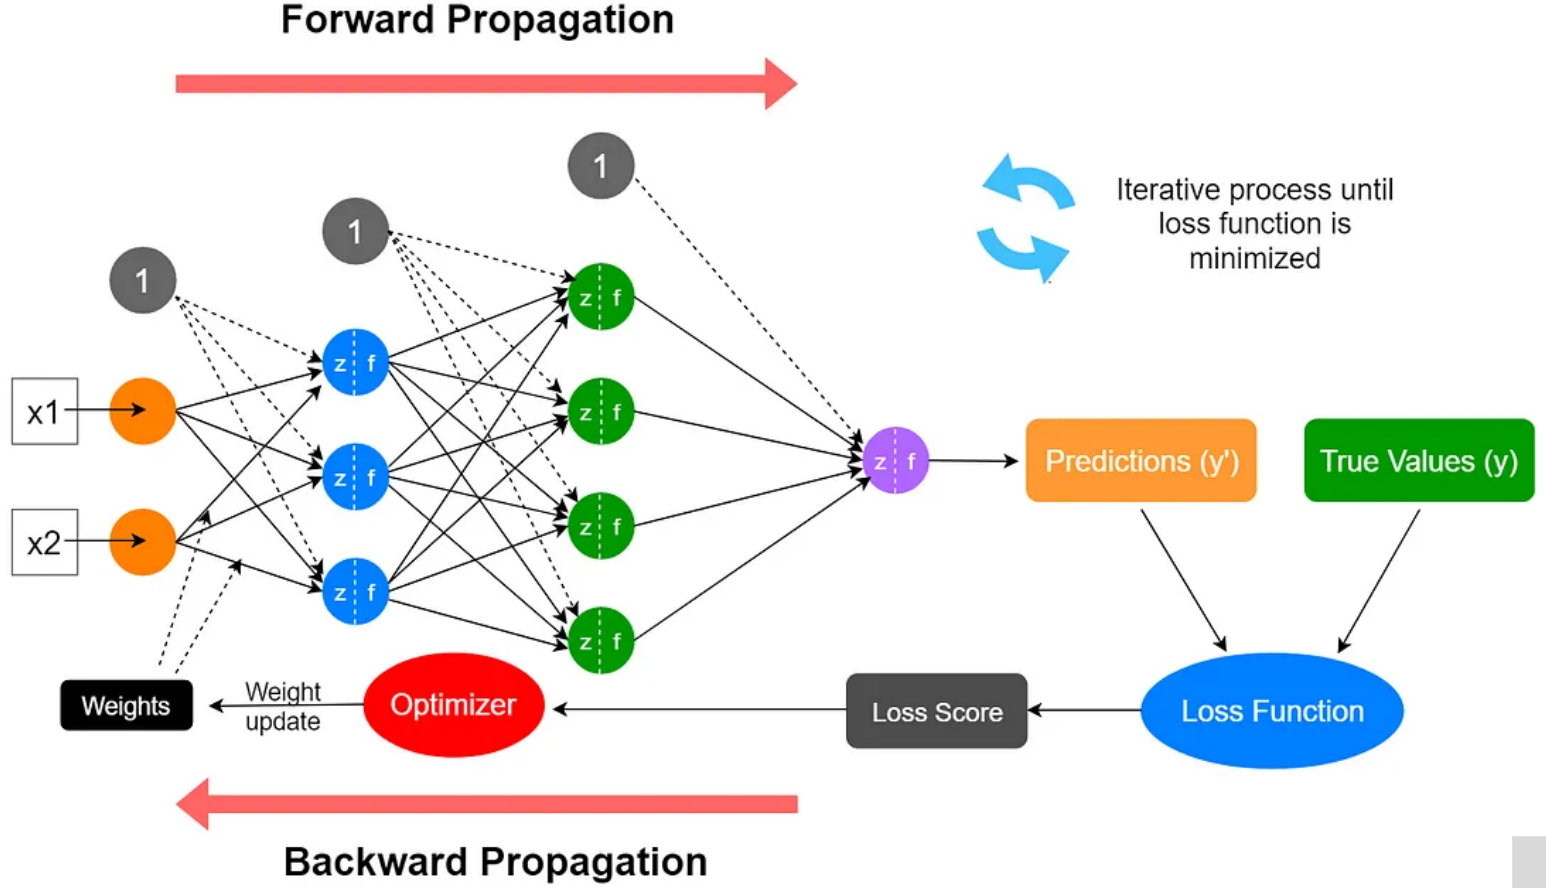
\includegraphics[width=0.95\linewidth]{fig/chap05-stats/dnn.png}
    \caption{Sketch of the training process of a binary classifier NN with 2 input features.}
    \label{fig:dnn}
\end{figure}




\subsection{Loss function}
Under the hood, a neural network is just an optimizer that tries to find the optimal function that minimizes a specific metric.\\
In other words, it is just a tool to perform a multidimensional fit, specifying the objective function in terms of sum and composition of activation function\footnote{This is called "induction bias" and is determined by the architecture of the NN}.\\
The metric that the NN tries to minimize during the learning phase is the so-called "Loss function", a continuous function that compares the prediction of the NN with the labels and has its minimum, ideally, when all the data are predicted correctly.\\
For example, in the case of a regression problem, one of the most used loss functions is the MSE $L=\sum(y_i-\hat{y_i})^2$, which is the same metric that is minimized when a least squares fit is performed.\\
\\
In the context of classification problems, the most used loss function is the cross-entropy loss.\\
Assuming that each class belongs to one output neuron, we can use the so-called one-hot encoding, which is a binary representation method where a categorical variable is transformed into a binary vector with a 1 indicating the presence of a particular category and 0s elsewhere\footnote{So, for example, if we have 3 classes, the 2nd class is represented with the vector [0,1,0]}.\\
So the output of the NN will be a vector as long as the total number of classes, and such that the sum of its elements is equal to 1. This can be achieved using the softmax activation function in the output layer (see the paragraph on activation functions).
\\
\\
The one-hot encoding representation is used, instead of the integer encoding that just indexes the classes, to avoid the assumption of natural ordering and to avoid predictions halfway between categories.\\
In the one-hot encoding representation, the cross-entropy loss is
\begin{equation}
    \mathcal{L}=-\sum_i^N w_{\hat{y}_i} \; \bm{\hat{y}_i} \cdot \log \bm{y_i}
\end{equation}
where $\bm{\hat{y_i}}$ and $\bm{y_i}$ are respectively the i-th label and prediction, both in the one-hot encoding representation, while $w_{\hat{y_i}}$ is a weight related to each class that is used to compensate the class imbalance in the training dataset, avoiding the NN to be biased towards one specific class.\\
\\
The cross-entropy loss is related to the likelihood of the multinomial distribution. Assuming m classes, the negative log-likelihood of the multinomial distribution, for a single data point, is\\
\begin{equation}
    -\log \mathcal{L}_{MN_{i}}(\bm{p_i};\bm{n_i})=-\sum_j^m n_j \log p_j + \text{const.}
\end{equation}
where $n_j$ is the number of predicted entries in the j-th class, and $p_j$ is the probability that the data belongs to the j-th class, and it's what depends on all the weight of the NN.\\
In the one-hot encoding representation $n_j=\delta_{j\hat{y}_i}$ and $p_j$ is the score ${y}_{\hat{y}_i}$, where $\hat{y}_i$ is the i-th label in the integer representation.
\begin{equation}
    \mathcal{L}_{MN_{i}}=-\bm{\hat{y}_i} \cdot \log \bm{y_i}
\end{equation}
Since each data point is independent from the others, the total log-likelihood is the sum of the single log-likelihoods
\begin{equation}
    \mathcal{L}_{MN}=-\sum_i \bm{\hat{y}_i} \cdot \log \bm{y_i}
\end{equation}

\subsubsection*{Optimizers and backpropagation}
To minimize the loss function, neural networks exploit the technique of gradient descent using different algorithms called "optimizers".\\
The simplest optimizer is the \textit{stochastic gradient descent} (SGD) that, for each data point, computes the gradient of the loss function and updates the weight in the opposite direction of the gradient, propagating it along the network in a procedure called \textit{back-propagation}\footnote{That is just a fancy name to call a composite derivative.}.
\begin{algorithm}
\caption{Stochastic gradient descent}\label{algo:SGD}
\begin{algorithmic}[1]
    \For{i=0 to T}
        \For{j=0 to len($\bm{x}$)}
            \State $\bm{w}=\bm{w}-\eta \grad_{\bm{w}} \mathcal{L}(y_j(\bm{w}),\hat{y}_j)$
        \EndFor
    \EndFor
\end{algorithmic}
\end{algorithm}\\
where $\eta$ is the \textit{learning rate} hyper-parameter.\\
The learning rate should be tuned carefully because a small learning rate will make the NN slow to reach the minimum of the loss, while a huge learning rate will make the gradient descent procedure very  unstable, jumping randomly across the loss hypersurface.\\
\\
To mitigate the fluctuation of the SGD and to improve the computational efficiency, we can compute the gradient on a batch of data and then update the weights
\begin{algorithm}[H]
\caption{Mini-batch stochastic gradient descent}\label{algo:miniSGD}
\begin{algorithmic}[1]
    \For{i=0 to T}
        \For{k=0 to $n_{\text{batch}}$}
            \State $\bm{w}=\bm{w}-\eta \grad_{\bm{w}} \sum_j^{\text{batch size}} \mathcal{L}(y_j^k(\bm{w}),\hat{y}_j^k)$
        \EndFor
    \EndFor
\end{algorithmic}
\end{algorithm}
In the most modern libraries, the gradient is computed and back-propagated using the \textit{automatic differentiation}.
In principle, when the NN is evaluated, a computational graph is built. The nodes of the graphs are just the operators applied to the tensors and, in the backpropagation phase, the gradients of each node are computed and propagated all the way along the graph using the chain rule.\\
Furthermore, NNs perform a lot of simple arithmetic operations that can be performed simultaneously in parallel. For this reason, the training and evaluation of NNs can be accelerated using graphing processing units (GPU).\\
\\
The list of optimizers is long and each of them has its pros and cons. The SGD has a slower convergence compared to the other optimizers due to its stochastic nature, it is really sensitive to the learning rate, and, especially in high-dimensional and nonconvex problems, it gets stuck very easily in local minima.\\
\\
To address these problems, one of the most used optimizers is ADAM (ADAptive Moment estimator) \cite{Kingma2014Adam:Optimization}. It is able to adapt the learning rate of each parameter individually computing the moving average of gradients and of square gradients, ensuring a fast convergence.
\\
The drawback of ADAM is that it has some convergence issues due to its large variance in the first epochs of training in the adaptive learning rate, showing huge fluctuations in the loss, and being too sensitive to the choice of hyperparameters.\\
Trying to stem these issues, recently, a new variant of Adam was proposed: RAdam (Rectified Adam) \cite{Liu2019OnBeyond}.\\
RAdam tries to tackle Adam's convergence issues by introducing a term to rectify the variance of the adaptive learning rate, trying to keep it small in the first epochs.

\begin{figure}[H]
    \centering
    \includegraphics[width=0.95\linewidth]{fig//chap05-stats/radam.png}
    \label{fig:radam}
\end{figure}
As the SGD, all the other optimizers can work on minibatch, evaluating the gradients on a group of data points.
\begin{figure}[H]
    \centering
    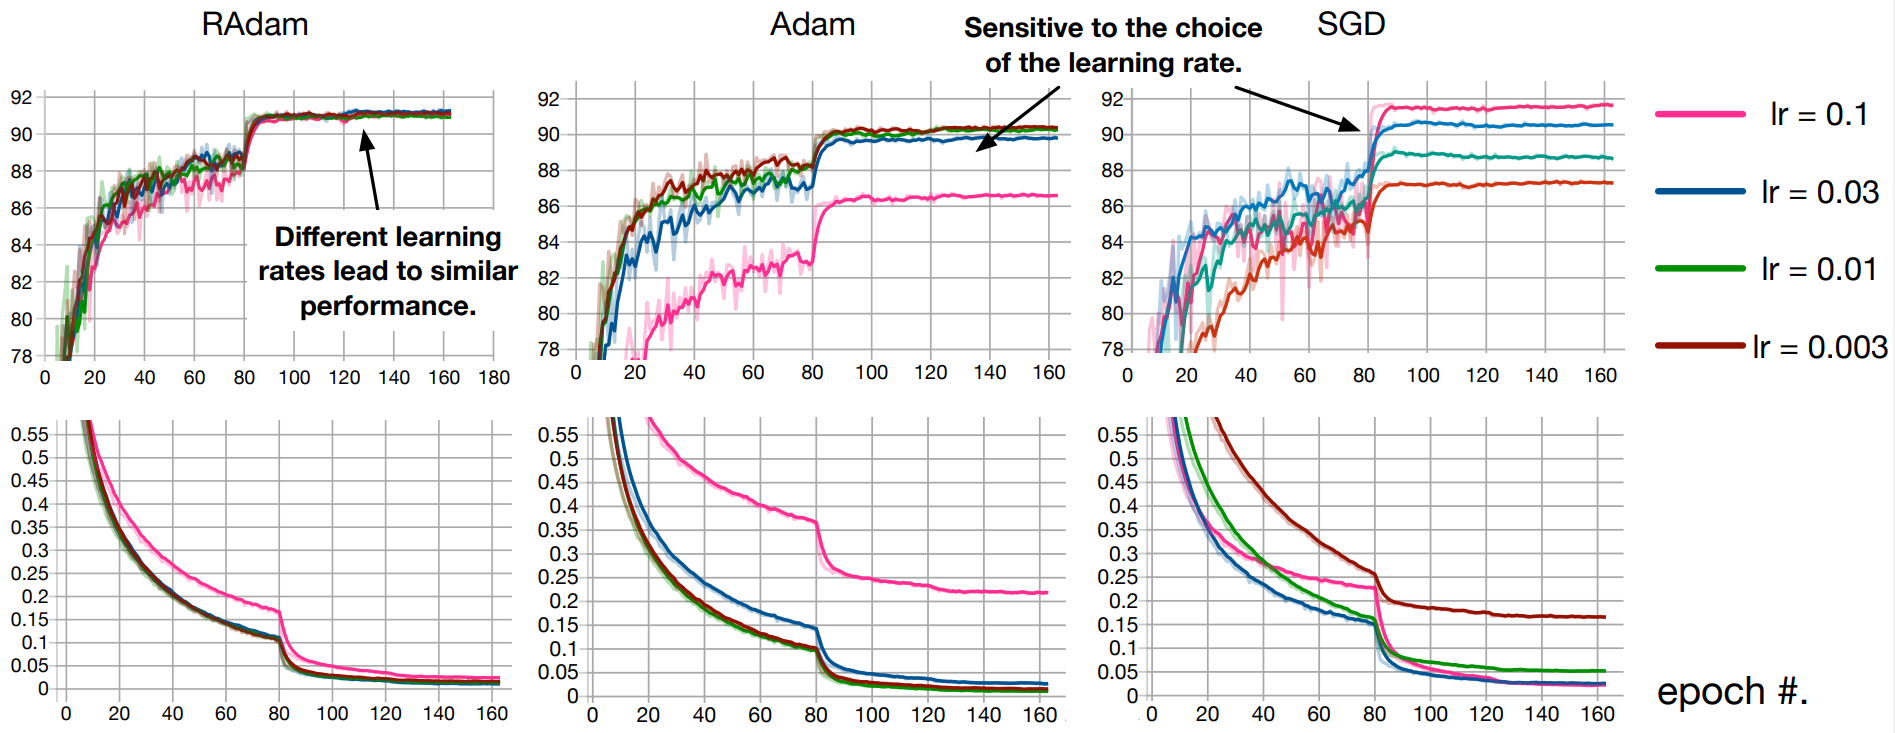
\includegraphics[width=\linewidth]{fig//chap05-stats/radam_loss.png}
    \caption{Evolution of the accuracy (top) and loss function (bottom) of RAdam, Adam, and SGD with different learning rates on the CIFAR10 problem \cite{Ho-Phuoc2018CIFAR10Humans} in the learning epochs \cite{Liu2019OnBeyond}.}
    \label{fig:radam_loss}
\end{figure}
\vspace{-1cm}
\subsection{Architecture and complexity}
The architecture of a neural network, specifically the number of layers and neurons, plays a crucial role in determining how well the network can learn and generalize from data.\\
A neural network can be shallow (few layers with many neurons) or deep (many layers with few neurons in each layer). \\
Deep networks tend to capture more complex patterns but suffer the vanishing gradient (the  magnitude of the gradient decreases propagating back in the network).\\
A high number of neurons improves the capacity to represent functions and makes the network more robust to the noise, embedding the data in a high-dimensional space.\\
Complex NNs are more prone to the \textit{overfitting}.
Overfitting is the behavior of an NN that occurs when the model performs well on the training dataset but doesn't perform in the same way on other data.\\
This occurs because the NN starts to learn the noise and the fluctuations of the training dataset, worsening its generalization capabilities and losing its predictive power.\\
During the training of an NN, overfitting is the most important thing to take under control, and, to do it, the loss is evaluated, for each epoch, not only for the data on which the network is training, but also for other data, called the "validation dataset".
\\
In the case of overfitting, we will see the validation loss that will start to increase, separating from the training loss.\\
On the other hand, if the network is too simple, we will fall into the underfitting, \ie the objective function represented by the NN is too simple to fit the data.
\vspace{-0.15cm}
\begin{figure}[H]
    \centering
    \includegraphics[width=1\linewidth]{fig/chap05-stats/overfit.jpg}
    \caption{Representation of underfitting, of a good fit, and of overfitting. The right plot shows the behavior of the validation loss in case of overfitting}
    \label{fig:overfitting}
\end{figure}

There are several techniques that can be used to prevent the overfitting:
\begin{itemize}
    \item Diminish the number of neurons and the complexity of the network
    \item Increase the size of the training dataset
    \item Add a penalty term to the loss function, like the L2 regularization
    \begin{equation}
        \mathcal{L}^{'}=\mathcal{L}+\lambda \sum ||\bm{w}||^2
    \end{equation}
    a term that penalizes scenarios in which the weights assume large values (that usually is one consequence of the overfitting)
    \item \textbf{Early stopping}: stop the learning when the validation loss has reached a plateau, before it starts to increase
    \item \textbf{Dropout}: the dropout \cite{Srivastava2014Dropout:Overfitting} is the probability that, in a single epoch during the training, one neuron will just be ignored and its connection with the rest of the network will be dropped out. \\
    By randomly disabling neurons, dropout prevents any single neuron from becoming overly specialized on a specific feature of the training data.\\
    Furthermore, introducing this stochastic behavior can also accelerate the training, preventing the network from getting stuck in local minima of the loss.\\
    The dropout rate is another hyperparameter that should be tuned carefully by the user.
\end{itemize}

\paragraph*{Residuals}\hspace{1cm}\\

\begin{minipage}{\linewidth}
    \vspace{0.1cm}
    \begin{minipage}{0.55\linewidth}
        To mitigate the effect of the vanishing gradient, some "skip connections" can be used to back-propagate the gradients better through the network, ensuring that the output of a layer is added together with the output of a later layer.\\
        If the dimensionality at the beginning of the connection is different from the dimensionality at the end of the connection, the residual can be multiplied by a linear projection to align the dimensions.\\
        These networks are called "residual networks" or ResNets \cite{He2015DeepRecognition}.
    \end{minipage}
    \hfill
    \begin{minipage}{0.4\linewidth}
        \centering
        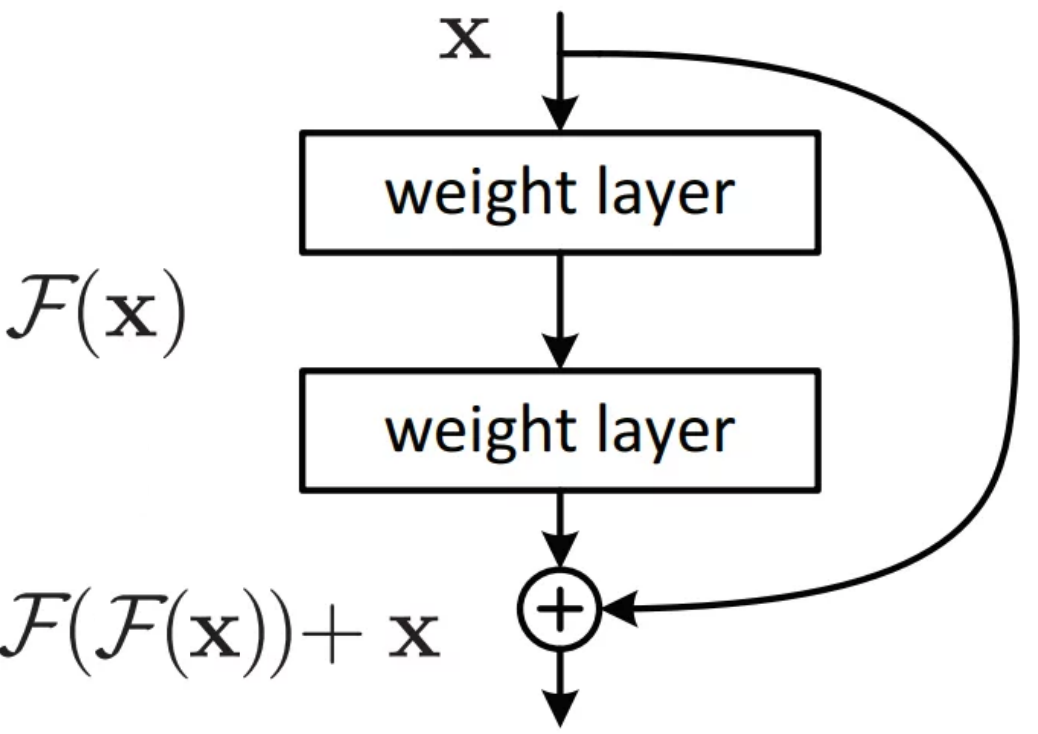
\includegraphics[width=1\linewidth]{fig/chap05-stats/res.png}
        \captionof{figure}{Visualization of the skip connection in a residual block of a ResNet.}
        \label{fig:resnet}
    \end{minipage}
\end{minipage}


\subsubsection*{Activation functions}
The activation functions in a neural network must possess some properties:
\begin{itemize}
    \item Continuity and differentiability: to compute the gradients of the loss with respect to the weights.
    \item Non-linearity: the activation functions must be non-linear because the composition of linear functions is still a linear function
    \item Their derivative must tend to a finite value for $x \to \pm \infty$ to avoid the so-called "explosive gradient", the opposite phenomena of the vanishing gradient.
\end{itemize}
The activation functions of the output layer are different from the others.\\
In a regression problem, the activation function of the output layer is a linear function, while, in the case of classification, using the one-hot encoding, the used activation function is the \textit{softmax} function
\begin{equation}
    {\textit{softmax} (\mathbf {x} )_{j}={\frac {e^{x_{j}}}{\sum _{k=1}^{K}e^{x_{k}}}}} \quad \text{for } j=1,\dots,K
\end{equation}
where K is the number of classes.\\
The softmax function ensures that the output of the network is a vector of length K, such that the sum of its elements is always 1. This allows us to threaten the output of the network as a probability.\\
\\
In the hidden layers, instead, we have more choices. The first activation functions ever used were the logistic function and the hyperbolic tangent, which are related to each other, and have a finite codomain.\\
These two functions were chosen due to the interpretation that we can give to them, like in the perceptron\footnote{in fact the logistic function can be seen as the "smoothed version" of the Heaviside theta function}: when the function is around its lower bound, the neuron is off, and when the function is around its upper bound, the neuron is on.
\begin{align}
    \tanh(x)&= \frac{e^x-e^{-x}}{e^x+e^{-x}}=2\sigma(2x)-1  \\
    \sigma(x)&=\frac{1}{1+e^{-x}} 
\end{align}
But the derivative of these functions is significantly different from zero just in a narrow range, slowing the learning of the network once the function saturates.\\
\\
Another activation function that was proposed was the ReLU (Rectified linear unit)\cite{FredAgarap2018DeepReLU}, one of the most used activation function
\begin{equation}
    \textit{ReLU}(x)=\max(0,x)
\end{equation}
The ReLU allows a better propagation of the gradients and is very efficient from the computational point of view since is a piecewise linear function and the gradient is a constant.\\
Furthermore, the ReLU introduces a sparse representation in the network:
when the network is initialized, only about half of the neurons have a non-zero output, and this has a regularization effect similar to the dropout.\\
Despite that, the ReLU suffers the so-called "dying ReLU problem": some units can be pushed into some states in which they become inactive to all possible inputs, making an always zero gradient. In this state, the neuron enters an endless dead state.\\
\\
To solve the dying ReLU problem, a lot of ReLU-like functions were proposed. In this work, the used activations function was the recently proposed Swish \cite{Ramachandran2017SearchingFunctions}. 
\begin{equation}
    \textit{Swish}(x; \beta)=\frac{x}{1+e^{-\beta x}}
\end{equation}
where $\beta$ is a learnable parameter.\\
The Swish function has a smooth gradient that can avoid the dying ReLU problem, ensuring the neurons continue to produce non-zero outputs.

\begin{figure}[H]
    \centering
    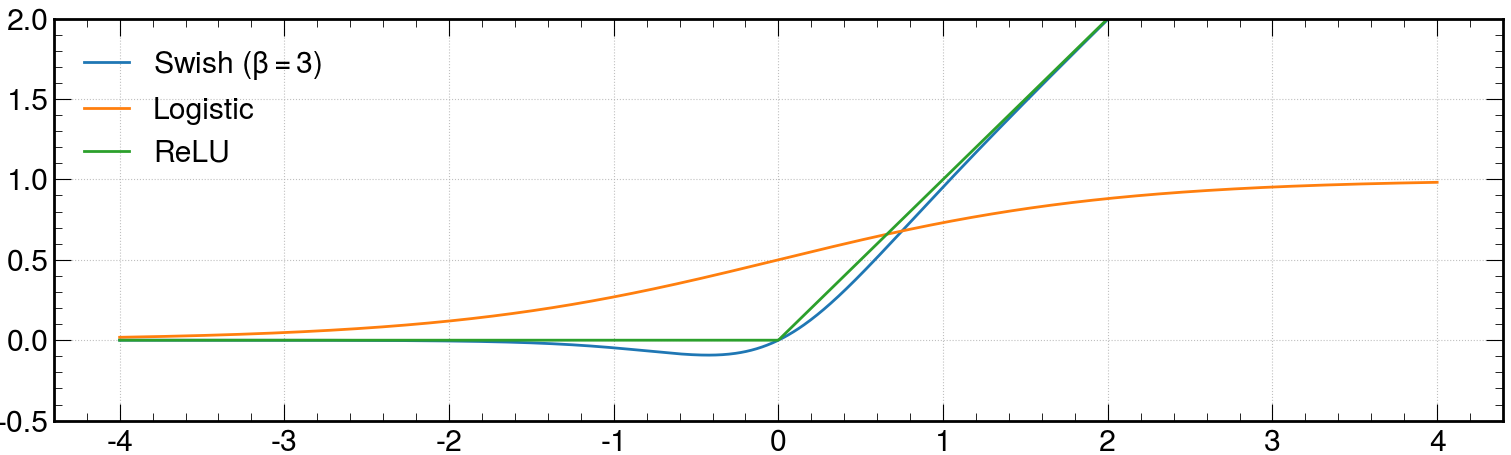
\includegraphics[width=0.85\linewidth]{fig//chap05-stats/act.png}
    \caption{Logistic, ReLU, and Swish activation functions.}
    \label{fig:activation}
\end{figure}

Anyway, despite all the motivations that were provided, the best activation function does not exist and, in general, in the field of neural networks, every choice is justifiable only through heuristics.


\subsubsection*{Input normalization}
The features of the input data have different distributions with different ranges and scales. The parameters associated with each feature will also have different scales and this can lead to a loss function whose gradient will be biased toward certain parameters, as shown in \Fig{fig:loss_normalization}.\\
\vspace{-0.5cm}
\begin{figure}[H]
    \hspace{-0.5cm}
    \centering
    \includegraphics[width=0.85\linewidth]{fig/chap05-stats/loss_norm.png}
    \vspace{0.5cm}
    \caption{Loss curve levels in case of non-normalized inputs (left) and normalized inputs (right) \cite{NormalizingNormalization.}.}
    \label{fig:loss_normalization}
    \vspace{-0.5cm}
\end{figure}
To make the learning of the network more stable and faster, we can normalize all inputs to a standard scale, allowing us to use larger learning rates.\\
Furthermore, this also avoids the saturation of a large number of activation functions in the first epochs which can lead to a slow learning due to the small gradients in the saturation regime.\\
For specific activation functions, like the ReLU-like, having inputs with zero mean will cause $\sim 50\%$ of the neurons to be inactive, creating a sparse representation (see paragraph on activation functions).\\
\\
One of the most used input normalization techniques is the \textit{Batch norm} \cite{Ioffe2015BatchShift}, which consists of normalizing each input feature with its mean and standard deviation computed across all the batch
\begin{equation}
    \bm{x}_i^{'}=\frac{\bm{x}_i-\mu_i}{\sigma_i+\epsilon}
\end{equation}
where $\bm{x}_i$ is the i-th feature of the input tensor and $\epsilon$ a small number added to prevent numerical issues.\\
\\
Despite that,  the mean and the standard deviations are not robust estimators, and, if a feature has significant outliers, the batch norm can create distributions not centered around zero.\\
To overcome this issue, we can replace the mean and the standard deviation with more robust estimators like the median, we can just clip the outlier to a threshold value, or we can apply a function that will shrink them.\\
In this work, the applied normalization to feature that has significant outliers is the following\footnote{$\bm{x_i}$ should be positive to apply this normalization}
\begin{equation}
    \bm{x}_i^{'}=\frac{\log \left(1+\bm{x}_i \right)-\mu_{i}^{\log}}{\sigma_i^{\log}+\epsilon}
\end{equation}
where $\mu_i^{\log}$ and $\sigma_i^{\log}$ are the mean and the standard deviation computed on $\log(1+\bm{x}_i)$

\paragraph*{Internal normalization}
During the training, the distribution of each layer’s weights changes, as the parameters of the previous layers change.
This slows down the training by requiring lower learning
rates. \\
This behavior is called "internal covariate
shift", and we can address the problem by introducing a normalizing layer in the network.\\
\\
We could use the batch norm or, instead, the layer norm \cite{Ba2016LayerNormalization}, which is the same thing as the batch norm but the mean and the standard deviation are computed across the features instead of across the batch.\\
In some architectures (like RNN) or domains (natural language processing), the layer norm was proven to work better than the batch norm.



\subsubsection*{Weight initialization}
The initialization of the weights is strictly related to the chosen normalization and to the chosen activation functions.\\
Large or small initialization values will lead respectively to the problem of exploding and vanishing gradient.\\
An appropriate initialization should impose a zero mean of the weights and a variance that should stay constant across all the layers.\\
\\
To do it, if we use activation functions that are linear around zero (like the $\tanh$), we can use the Xavier initialization \cite{Glorot2010UnderstandingNetworks}.
\begin{equation}
    W\sim U \left[-\frac{\sqrt{6}}{\sqrt{n_j+n_{j+1}}},\frac{\sqrt{6}}{\sqrt{n_j+n_{j+1}}} \right]
\end{equation}
where $n_j$ is the number of units in the j-th layer.\\
If we use ReLU-like functions, instead, we should use the He initialization \cite{he2015delving}.
\begin{equation}
    W\sim \mathcal{N}\left(0,\frac{2}{n^l}\right)
\end{equation}
the derivation of these two distributions is simple and is provided in the respective papers, and consists only of imposing the variance of the output of a unit to be constant across all layers.

\subsubsection*{Hyperparameter optimization}
In this section, we have introduced many hyperparameters like the learning rate, the size of the network, etc. These parameters have to be tuned to obtain the best performances.\\
\\
The simplest way to perform a hyperparameters search is to perform a \textit{grid seach}, which consists of creating a grid of parameters and repeating the training for each combination of them.\\
However, this simple algorithm is feasible only for small networks because the number of trainings required depends on a combinatorial factor.\\
\\
Clever ways to find the optimal set of hyperparameters can involve Bayesian optimization methods, but, if the model is too big and the time and the computing resources are very scarce, the only remaining tool is manual optimization in which the user tries to find a good set of hyperparameters by trying with just a couple of trainings.


\subsection{Attention mechanism}
Attention is a mechanism that enables models to focus on specific parts or elements of the input data while performing a task.\\
It is particularly important in fields like natural language processing (NLP) and computer vision.\\
\\
Attention networks belong to the class of sequence-to-sequence (seq2seq) models. 
One of the most common seq2seq tasks is the language translation in which the model takes as input one sentence (\ie a sequence) in a language and translates it into another language (\ie another sequence).
This means that the inputs of the network are 3 dimensional: one is the batch dimension, one is the sequence dimension, and the last is the feature dimension.\\
In particle physics, seq2seq models enable us to threaten each event as a sequence composed of its particles and to maintain its structure.

\subsubsection*{Scaled dot product}
One particular method to implement the attention is the scaled dot product \cite{Vaswani2017AttentionNeed}.\\
\begin{equation}
    \textit{Attention}(Q,K,V)=\textit{softmax}\left(\frac{QK^T}{\sqrt{d_k}}\right)V
\end{equation}
\vspace{0.2cm}\\
The scaled dot product has 3 inputs: the Query of dimensions $(N, S_2, d_k)$ and Key of dimension $(N, S_1, d_k)$, and the Value of dimension $(N, S_2, d_v)$, where $N$ is the batch size, and $S_1,S_2$ the length of the sequences.\\


\begin{minipage}{\linewidth}
    \begin{minipage}{0.53\linewidth}
        $Q,K,V$ are linear embeddings of the inputs, so $Q,K,V=W_{Q,K,V} \cdot X_{Q,K,V}$ where $W$ are the weights learned during the training.\\
        \\
        The dot product is used to compute a similarity score between the query and key vectors, weighting $V$ with it.\\
        $\textit{softmax}\left(\frac{QK^T}{\sqrt{d_k}}\right)$ has dimension $(N,S_2,S_1)$, so it assigns a score to all the pairs in the two sequences.\\
    \end{minipage}
    \hfill
    \begin{minipage}{0.43\linewidth}
        \vspace{-0.7cm}
        \centering
        \includegraphics[width=0.5\linewidth]{fig//chap05-stats/translation.png}
        \vspace{0.6cm}
        \captionof{figure}{Attention scores between sentences in English and French. The network has learned to recognize which words have the same meaning also if they are in a different order.}
        \label{fig:Translation}
    \end{minipage}
\end{minipage}
\vspace{0.1cm}\\
Attention networks are a rare example of explainability. By studying attention scores we can understand what the network is learning. Usually, instead, neural networks are black boxes that tend to learn representations that are difficult to understand by humans.
\\
\\
In particle physics, this approach is particularly feasible for two reasons
\begin{itemize}
    \item There is a natural way to handle missing elements in the sequence: we can just fix the maximum length of the sequence and, for the missing particles, just impose the respective attention scores to zero.\\
    This allows us to maintain the ragged structure of the event.
    \item Attention networks are invariant for permutation of the elements in the sequence, so we are not forced to introduce an ordering between the particles
\end{itemize}


\paragraph*{Multihead attention}
One set of $W_Q,W_K,W_V$ matrices is called an \textit{attention head}, but we can stack multiple attention heads together, allowing the model to attend parts of the sequence differently.\\
The different heads can be computed in parallel and their output, at the end, is concatenated.

\begin{figure}[h!]
    \centering
    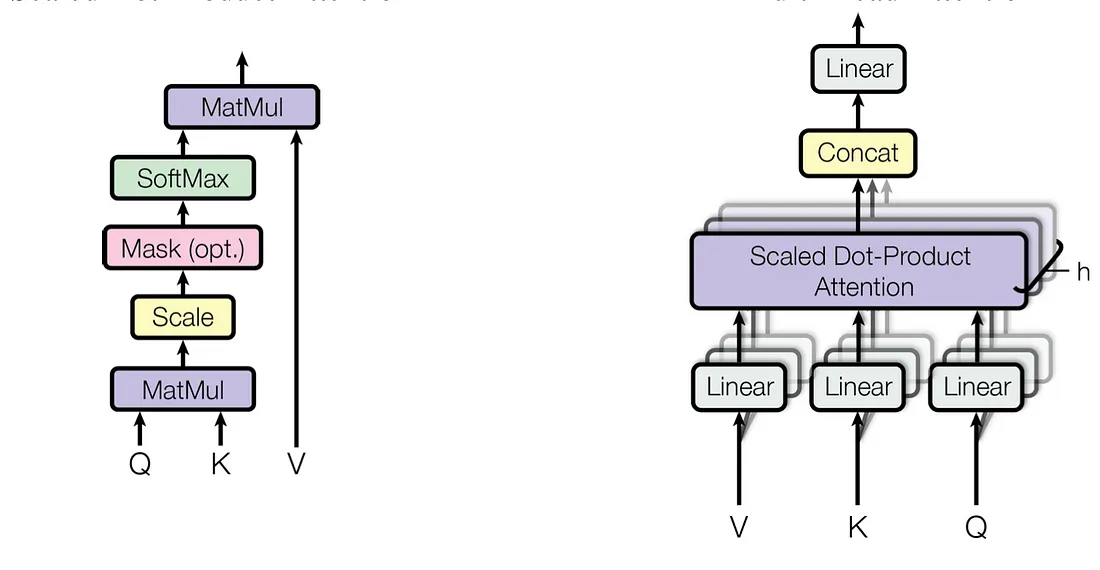
\includegraphics[width=0.75\linewidth]{fig//chap05-stats/multihead_attention.png}
    \caption{(Left) scaled dot product, (right) multi-head attention}
    \label{fig:multihead}
\end{figure}

\paragraph*{Self-attention} With a "self-attention layer" we refer to a scaled dot product layer in which $Q,K,V$ are linear embeddings of the same input $\bm{X}$.\\
It enables the model to capture contextual information and relationships between elements in the sequence, computing attention scores for each element with respect to all the others.\\
These attention scores determine how much each element should focus on the others and the resulting weighted sum provides a contextually enriched representation of the sequence.

\paragraph*{Cross-attention}
Cross-attention is an extension of the self-attention mechanism that allows a model to attend to elements in a target sequence based on the elements in another sequence (called context sequence).\\
The Key and Value vectors are linear embeddings of the context sequence while the Query is a linear embedding of the target sequence.\\
Cross-attention allows models to establish relationships between elements in different sequences, also of different lengths, making it suitable for tasks that involve aligning information from one sequence with another.

\paragraph*{Self-attention pooling}


Pooling is a technique used to downsample or reduce the dimensionality of feature maps or, in our case of a sequence, retaining important information.\\
As already discussed, we are interested in classifying an event as a signal or background, so we have to reduce the dimensionality of the sequences that contain all the particles in the events, to just one.\\
Self-attention pooling \cite{Safari2020Self-attentionRecognition} is a pooling layer inspired by self-attention
\begin{equation}
    \textit{Self-Att. Pool}=\textit{Softmax}(\bm{W} \bm{X}^T)\bm{X}
\end{equation}
where $\bm{X}$ is the input tensor of size $(N,S,F)$ and $\bm{W}$ is a set of trainable weight of size $S^{'},F$, where $S^{'}$ is the target size of the output sequence.\\
Therefore, self-attention pooling is a weighted average of the sequence features where the weights correspond to the alignment learned by the self-attention mechanism.













%%%%%%%%%%%%%%%%%%%%%%%%%%%%%%%%%%%%%%%%%%%%%%%%%%%%%%%%%%%%%%%%%%%%%%%%%%%%%%%
%%%%%%%%%%%%%%%%%%%%%%%%%%%%%%%%%%%%%%%%%%%%%%%%%%%%%%%%%%%%%%%%%%%%%%%%%%%%%%%
%%%%%%%%%%%%%%%%%%%%%%%%%%%%%%%%%%%%%%%%%%%%%%%%%%%%%%%%%%%%%%%%%%%%%%%%%%%%%%%
%%%%%%%%%%%%%%%%%%%%%%%%%%%%%%%%%%%%%%%%%%%%%%%%%%%%%%%%%%%%%%%%%%%%%%%%%%%%%%%
\newpage
\section{Signal extraction}
\subsection{Likelihood construction}Signal
The signal extraction procedure relies on a maximum likelihood fit of a binned distribution of one or more observables.\\
The likelihood is constructed as the product of Poisson distributions, one for each bin, that contains the parameter of interest (POI) to fit.\\
Given $C$ channels\footnote{A channel is defined by a set of cuts and selections that have the scope to isolate the signal and reject the background or viceversa}, each that contains $P_c$ processes, represented with histograms with $B_c$ bins, once we have the signal and the background MC predictions $s_{cb}$, $b_{cb}$, and the observed bin content $n_{cb}$ \footnote{Index $c$ stands for "channel", $p$ for "process", $b$ for "bin"}, the likelihood is \cite{Khachatryan2015PreciseTeV}
\begin{equation}
    \mathcal{L}(\mu)=\prod_c^C \prod_b^{B_c} \frac{(\mu s_{cb}+b_{cb})^{n_{cb}}}{n_{cb}!} e^{-(\mu s_{cb}+b_{cb})}
\end{equation}
In this case, the POI is the signal strength $\mu$, which is estimated by finding the value that maximizes the likelihood. The optimization problem is solved using the \textsc{MIGRAD} algorithm \cite{James1998MINUIT:Manual}, implemented in the \textsc{MINUIT2} library, that performs a line search in the direction of the gradient and updates the covariance matrix (inverse of the Hessian matrix) with each step.\\
To improve the numerical stability, the software implementation exploits the negative log-likelihood $\textit{NLL}=-\log{\mathcal{L}}$ instead of the likelihood in the form of the \Eq{eq:likelihood}  
\begin{equation*}
    \hat{\mu}=argmin_\mu - \log{\mathcal{L}(\mu)}
\end{equation*}
The predictions for each process are obtained through MC simulations, that are rescaled to match the total number of expected observed events. If $N^{MC}_{cp}$ is the total number of entries in the histogram relative to the process $p$ in the channel $c$, the respective entries have to be rescaled by a factor $w_{cp}$
\begin{equation}
    w_{cp}=\frac{\mathcal{L_I} \sigma_p \epsilon_{cp}}{N_{cp}}
\end{equation}
where $\mathcal{L_I}$ is the integrated luminosity, $\sigma_p$ the cross-section of the process $p$ and $\epsilon_{cp}$ the fraction of events of the process $p$ that pass the preselection defined by the channel $c$ that is estimated using MC events. 
\\
\newpage
\subsubsection*{Systematic uncertainties}
To incorporate in the model all the relevant uncertainties (\ie luminosity and rate uncertainties, uncertainties related to the detector resolution, etc.) we add to the likelihood the so-called nuisance parameters $\vec{\theta}$.\\
The likelihood becomes \cite{Conway2011IncorporatingSpectra}
\begin{equation}\label{eq:likelihood}
    \mathcal{L}(\mu,\vec{\theta})=\prod_c^C \prod_b^{B_c} Poiss \big( n_{cb}| \lambda_{cb}(\mu,\vec{\theta}) \big)  \prod_k  \pi_{k}(\theta_k)
\end{equation}
where $\pi_{k}$ is the prior probability distribution of the nuisance $\theta_k$.\\
The expectation value $\lambda_{cb}$ of the Poisson distribution now depends on the nuisance parameters that can be classified into normalization nuisances, shape nuisances, and statistical nuisances.
\begin{equation}\label{eq:lambda}
     \lambda_{cb}( \mu,\vec{\theta})=\sum_p^{P_c}M_{cp}(\mu) N_{cp}(\vec{\theta}_n)y_{cpb}(\vec{\theta}_s)+E_{cb}(\vec{\theta}_{MC})
\end{equation}
The term $M_{cp}(\vec{\mu})$ is the physical model that contains the POI to fit, $N_{cp}(\vec{\theta_n})$ contains the factors relative to normalization nuisances, $y_{cpb}(\vec{\theta}_s)$ is the predicted content of each bin (that depends on shape nuisance parameters) and $E_{cpb}(\vec{\theta}_{MC})$ represents bin per bin the statistical error of the Monte Carlo predictions.\\
In the absence of systematic uncertainties, we have $N_{cp}=1$ and $E_{cb}=0 \quad \forall c,p,b$ and
$M_{cp}=\mu$ if $p$ is a signal process, otherwise $M_{cp}=1$; while $y_{cpb}$ is just the predicted bin content for each process.\\
All the nuisance parameters $\theta_k$ are defined in units of standard deviations\footnote{it means that $\theta=\pm 1$ correspond to a $\pm 1 \sigma$ variation.}.\\
Given that we know the central values and the standard deviations of all the variations, following the maximum entropy principle \cite{Jaynes2003ProbabilityScience}, we can use the normal distribution as a prior for all the nuisance parameters.
\begin{equation}
    \pi_k(\theta_k)=\mathcal{N}\left(\theta_k|0,1\right)=\frac{1}{\sqrt{2\pi}}e^{-\theta_k^2/2}
\end{equation}
\begin{itemize}
    \item \textbf{Normalization nuisances} are multiplicative corrections that affect the normalization of one process (\eg the cross-section uncertainties) or of all processes (\eg the luminosity uncertainties).\\
    This type of uncertainty does not change the shape of the histogram but changes the number of expected events.\\
    In $\lambda_{cb}$ [eq. \ref{eq:lambda}], they are represented by the term
    \begin{equation}
        N_{cp}\left(\vec{\theta}_n\right)=k_{cp}^{\theta^{(n)}_k}
    \end{equation}
    where $k_{cp}$ the relative $+1 \sigma$ variation from the nominal event yield for the process $p$ in the channel $c$ estimated through theory calculation of external measurements, while $\theta_{k}$ is the relative normalization nuisance parameter.\\
    \newpage
    \item \textbf{Shape nuisances}: Shape-changing nuisances are produced by uncertainties
    that cause a different variation of event yields for each different bin.\\
    The model parameters are varied of $\pm 1 \sigma$ around their central value, creating an “Up” and a “Down” variation.\\
    The bin content $y_{cpb}$ has to be modified by multiplying a continuous and differentiable function of $\vec{\theta}_{s}$, so, given $\delta_b^\pm$ the differences between the $\pm 1 \sigma$ bin content variations of the bin and the nominal one, the up and down variations are interpolated with a spline in a procedure called "vertical morphing" \cite{Conway2011IncorporatingSpectra}
    \begin{equation}
    f_b\left(\theta_k^{(s)}\right)=
        \begin{cases}
            {\frac{1}{2}}\left((\delta_b^{+}-\delta_b^{-})\theta_k+{\frac{1}{8}}(\delta_b^{+}+\delta_b^{-})(3\theta_k^{6}-10\theta_k^{4}+15\theta_k^{2})\right) & \text{for } |\theta_k|\leq 1\\
            \theta_k \delta^+ & \text{for } \theta_k>1\\
            -\theta_k \delta^{-} & \text{for } \theta_k<-1
        \end{cases}
    \end{equation}
    The term $y_{cpb}(\vec{\theta}_s)$ is then defined as 
    \begin{equation}
        y_{cpb}(\theta_s)=max\left(0,y_{cpb}+\sum_k f_{cpb}\left(\theta_k^{(s)} \right)\right)
    \end{equation}
    In this way, we can clip $y_{cpb}$ to 0 preventing the height of the bin from being negative.\\
    The vertical morphing procedure is shown and described in detail in \Fig{fig:morphing}



    
    \item \textbf{MC statistical nuisances}: The MC events used to predict the expected signal and background yield in each bin are limited.\\
    To model the statistical MC uncertainties, we could add a nuisance parameter per bin per process, following the Barlow-Beeston approach \cite{Barlow1993FittingSamples}.\\
    But, if we have enough statistics in each bin, we can just use a nuisance parameter per bin that scales the sum of the processes yield, following the Barlow-Beeston lite approach \cite{Barlow1993FittingSamples}.\\
    The term $E_{cb}$ in $\lambda_{bc}$ is the term related to the statistical uncertainties is
    \begin{equation}
        E_{cb}(\vec{\theta}_{MC})=\theta_b\left(\sum_p \left(e_{cpb}N_{cp}(\vec{\theta}_n)M_{cp}(\mu)\right)^2 \right)^{1/2}
    \end{equation}
    where $N_{cp}$ and $M_{cp}$ are the normalization factor and the physical model defined before.
    $e_{cpb}$ is the Poissonian standard deviation of the b-th bin in the process p. Considering that the $\hat{\sigma}_{Poiss}=\sqrt{y_b}$ and that the bin height has to be rescaled to match the expected number of observed events, $e_{cpb}$ is
    \begin{equation}
        e_{cpb}=w_{cp} \sqrt{N_{cpb}^{MC}}   =\frac{\mathcal{L_I} \sigma_p \epsilon_{cp}}{N^{MC}_{cp}} \sqrt{N^{MC}_{cpb}}
    \end{equation}
    where $N_{cpb}$ is the number of MC events in the b-th bin.\\
    The term $E_{cb}$ scales, linearly with the nuisance parameter, the event yield of the bin with the root square sum of the Poisson uncertainties of each process.\\
\end{itemize}
\begin{figure}[h!]
    \centering
    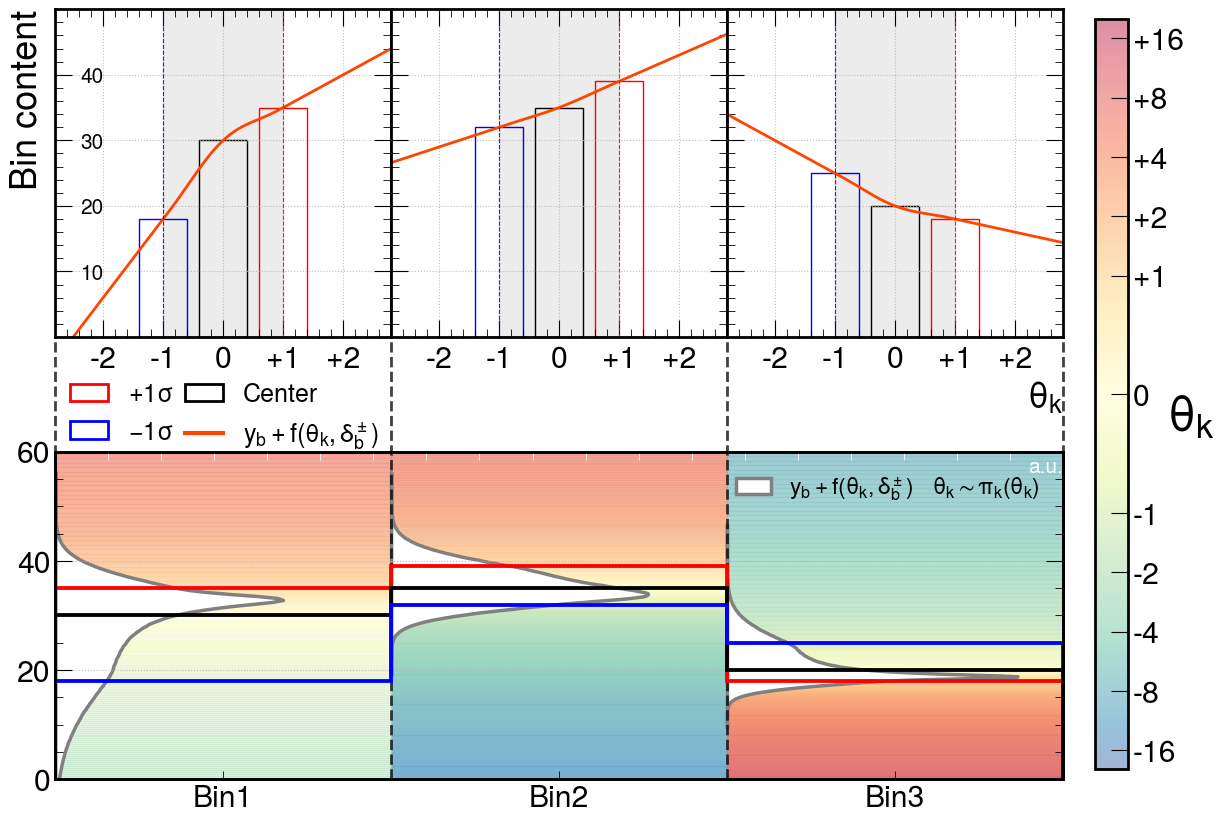
\includegraphics[width=\linewidth]{fig//chap05-stats/morphing.png}
    \caption{In the lower panel is represented an example of a histogram with 3 bins. The black line represents the histogram, the blue and the red lines represent the $\pm 1 \sigma$ shape variations.
    In the top panel, each bin is represented with its $\pm 1 \sigma$ variations and, on top of them, the $y_b+f(\theta_k,\delta_b^\pm)$ interpolation is shown with a red line. In the background of the lower panel, a color map shows, for each value of the bin height, the corresponding value of the nuisance parameter $\theta_k$, while the rotated vertical white shadow represents, for each bin, the probability distribution in arbitrary units of the expectation value of the Poisson distribution $\lambda_b=y_b+f(\theta_k,\delta_b^\pm)$ drawing $\theta_k$ from the normal prior.}
    \label{fig:morphing}
\end{figure}
\newpage
\vspace{0.5cm}
\paragraph*{Smoothing}
For some systematics, up and down variations can lead to significant statistical fluctuations in the less populated bins, which, usually, are the high signal purity regions of the histogram.\\
To overcome this inconvenience, a smoothing procedure is applied.

\begin{algorithm}[H]
\caption{Smoothing algorithm}\label{algo:smooth}
\begin{algorithmic}[1]
    \State Compute $r^{up}_b=y_{b}^{up}/y_b$ and $r^{down}_b=y_{b}^{down}/y_b$
    \State Compute $\delta r_b=\left(r^{up}_b-r^{down}_b\right)/2$
    \State Define $\hat{r}^{up}_b=1+\delta r_b$ and $\hat{r}^{down}_b=1+\delta r_b$
    \State Given $x_b$ is the position of the bin centers, apply the LOWESS smoothing algorithm to the points $(x_b,\hat{r}^{up}_b)$ and $(x_b,\hat{r}^{down}_b)$, finding the functions $f^{up}(x)$ and $f^{down}(x)$
    \State Redefine $y_b^{up}=y_b f^{up}(x_b)$ and $y_b^{down}=y_b f^{down}(x_b)$
\end{algorithmic}
\end{algorithm}
\\
The LOWESS algorithm \cite{Cleveland1979RobustScatterplots} (LOcally WEighted Scatterplot Smoothing) performs different linear regressions on a sliding window in different steps.


\begin{algorithm}[H]
\caption{LOWESS algorithm}\label{algo:LOWESS}
\begin{algorithmic}[1]

    \State For each point $(x_i,y_i)$, create a window of a fixed length L.
    \State Define the weights $w_{1,ij}(x)=(1-|(x_j-x_i)/L|^3)^3 \; \Theta(L-|x_j-x_i|)$ where $\Theta$ is the Heaviside theta function.
    \State Perform a linear regression in each window, weighting each point with the defined weights $w_{1,ij}$. 
    \State Define $\hat{y}_i=f_{1,i}(x_i)$ where $f_{1,i}$ is the linear function obtained from the linear regression in each window.
    \State Compute the residuals $s_i=|y_i-\hat{y}_i|$.
    \State Normalize the residuals with $s_i=s_i/(6 m(s_i))$ where $m(s_i)$ is the median of the residuals.
    \State Define the weights $w_{2,i}=(1-s_i^2)^2 \; \Theta(1-s_i)$ 
    \State Perform a second linear regression on the points $(x_i,\hat{y}_i)$ weighting each point in the window with $w_{2,i}$, obtaining the functions $f_{2,i}$
    \State The smoothed curve is $(x_i,f_{2,i}(x_i))$

\end{algorithmic}
\end{algorithm}


\subsection{Profile Likelihood}
According to Wilks' theorem \cite{James2006StatisticalEdition}, the distribution of the likelihood ratio is asymptotically distributed like a $\chi^2$.
\\
We have to fit just the POI $\mu$, so we can define the profile likelihood
\begin{equation}
    -2 \Delta \ln(\mathcal{L})=-2 \ln{\lambda(\mu)}= -2 \ln \left( \frac{\mathcal{L}(\mu,\bm{\tilde{\theta}}(\mu))}{\mathcal{L}(\hat{\mu}, \bm{\hat{\theta}})}\right) \sim \chi^2_1(\mu)
\end{equation}
$\hat{\mu}$ and $\bm{\hat{\theta}}$ are the parameters that maximize the likelihood simultaneously, while $\bm{\tilde{\theta}}(\mu)$ are the values of the nuisance parameters that maximize the likelihood for a fixed value of $\mu$.\\
Since $\int_0^1\chi^2_1(x) dx =0.683 = 1\sigma$, to compute the 68\% confidence level (CL) on $\hat{\mu}$, we can compute the profile likelihood and find the values of $\mu$ for which holds $-2\Delta \ln{\mathcal{L}(\mu)}=1$.\\
\\
To understand how different groups of nuisances affect the profile likelihood and the total uncertainty on $\mu$, some of the $\bm{\tilde{\theta}}(\mu)$ can be frozen in turn to the values $\bm{\hat{\theta}}$.\\
The so-called "breakdown procedure" consists of freezing sequentially groups of nuisance parameters, computing the profile likelihood and the relative uncertainties, and subtracting them in quadrature from the total uncertainty.


\paragraph*{Impact plots} Impact plots are a useful tool to understand the impact that each nuisance has on the total uncertainty. An example is shown in \Fig{fig:impact}.\\
\begin{itemize}
    \item In the left panel there are the names of the systematic sources, sorted according to their impact on the total uncertainty.
    \newpage
    \item In the center panel, there are two elements:
    \begin{itemize}
        \item[\ding{226}] The black bars ("Fit") represent the profile likelihood of the nuisance parameter. For each nuisance
        \begin{equation}
             \hat{\theta}_k=argmin_{\theta_k} -2 \ln \left( \frac{\mathcal{L}(\theta_k, \tilde{\mu}(\theta_k),\bm{\tilde{\theta}}(\theta_k))}{\mathcal{L}(\hat{\mu},\bm{\hat{\theta}},\hat{\theta}_k)} \right)
        \end{equation}
        is computed, along with the respective uncertainty, exploiting Wilks' theorem as explained before.
        \item[\ding{226}] The blue crosses ("Pulls") corresponds to $(\hat{\theta}-\theta_{\text{pre-fit}})/\sqrt{\sigma_{\text{pre-fit}}^2-\sigma_{\text{post-fit}}^2}$.\\
        They tell us how much the fitted values are in tension with the pre-fit values defined by the priors.      
    \end{itemize}
    \item In the right panel there are the impacts.
    Once we have the fit for each nuisance, we can perform again the profile likelihood procedure on $\mu$ but fixing each nuisance in turn to their $\pm 1 \sigma_{\text{post-fit}}$ value. The blue and the red bars represent the values $\Delta^{\pm} \hat{\mu}=\hat{\mu}(\hat{\theta})-\hat{\mu}(\hat{\theta}_{\pm 1 \sigma})$.    
\end{itemize}
\begin{figure}[h!]
    \centering
    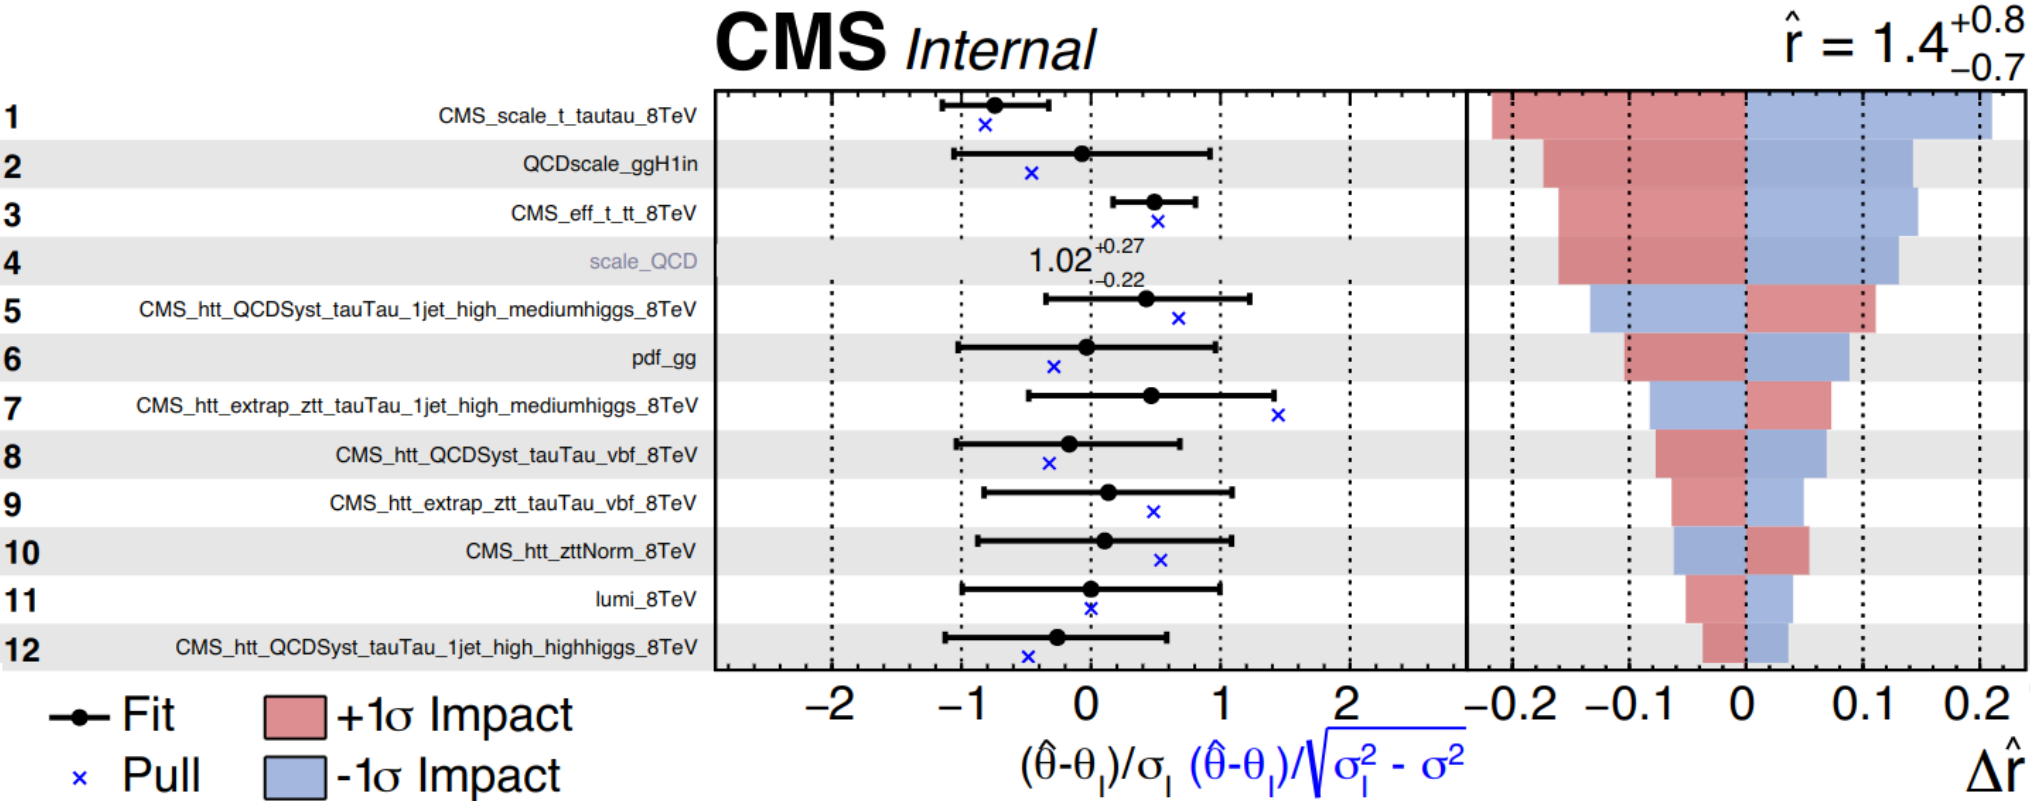
\includegraphics[width=1\linewidth]{fig/chap05-stats/impact.png}
    \caption{Example of an impact plot. In this plot, the POI $\mu$ is called $r$, and $\theta_I$, $\sigma_I$ are the pre-fit values.}
    \label{fig:impact}
\end{figure}


\subsection{Asimov dataset and significance} The term $n_{cb}$ in \Eq{eq:likelihood} is the number of observed events in the b-th bin, so, it contains real data.\\
To perform a simulation of an analysis, $n_{cb}$ can be replaced by MC events, creating the so-called "Asimov dataset" \cite{Cowan2011AsymptoticPhysics}
\begin{equation}
    n_{cb}^{\text{Asimov}}=\sum_p y_{cpb}
\end{equation}
In this way will be always $\hat{\mu}=1$ and $\bm{\hat{\theta}}=0$.\\
Using the Asimov dataset, the statistical uncertainties on $\hat{\mu}$ can be estimated through an approximation.
\newpage
\begin{enumerate}
    \item Let's consider the Poisson log-likelihood for a single bin
\begin{equation}
    \ln\left(\mathcal{L}_b(\mu)\right)=n_b \ln(\mu s_b + b_b) - (\mu s_b + b_b)-\ln n_b! 
\end{equation}
and let's find the maximum likelihood estimator for $\mu$
\begin{equation}
    \partial_\mu \ln{\mathcal{L}_b}=0 \implies \hat{\mu}=\frac{n_b-b_b}{s_b}
\end{equation}
The variance of the estimator $\hat{\mu}_b$ is
\begin{equation}
    {\mathrm{Var}}(\hat{\mu}_b)=\frac{{\mathrm{Var}}(n_b)}{s_b^2}=\frac{\mu s_b + b_b }{s_b^2}
\end{equation}
The variance of $\hat{\mu}_b$ depends on $\mu$ itself, but, in the context of the Asimov dataset, we can approximate it imposing $\mu=\hat{\mu}_b=1$, so the variance becomes
\begin{equation}
    {\mathrm{Var}}(\hat{\mu}_b)\sim \frac{s_b+b_b}{s_b^2}
\end{equation}
 \item The Cramer-Rao theorem \cite{James2006StatisticalEdition} states that, for a probability density function of the exponential family, to whom the Poisson distribution belongs, it holds
\begin{equation}
    \mathrm{Var}(\hat{\mu})=-\frac{(1-\partial_\mu b)^2}{E[\partial_\mu^2 \ln \mathcal{L}]}
\end{equation}
where $b$ is the bias of the estimator.
The maximum likelihood estimator is asymptotically unbiased, so we can neglect $b$.
\begin{equation}
    E[\partial_\mu^2 \ln \mathcal{L}_b]\sim-\frac{1}{\mathrm{Var}(\hat{\mu}_b)}
\end{equation}
and for the total likelihood
\begin{equation}
    E[\partial_\mu^2 \ln \mathcal{L}]=
    \sum_b E[\partial_\mu^2 \ln \mathcal{L}_b]=\sum_b
    -\frac{1}{\mathrm{Var}(\hat{\mu}_b)}
\end{equation}
but since it holds $\mathrm{Var}(\hat{\mu}) =-1/E[\partial_\mu^2 \ln \mathcal{L}]$, then
\begin{equation}
    \mathrm{Var}(\hat{\mu})=\left[\sum_b \frac{1}{\mathrm{Var}(\hat{\mu}_b)}\right]^{-1}= \left[\sum_b \frac{s_b^2}{s_b+b_b} \right]^{-1}
\end{equation}
\end{enumerate}
So, to estimate the uncertainty on $\hat{\mu}$ using the Asimov dataset, we can compute the so-called \textbf{significance}
\begin{equation}
    Q=\sum_c \sum_b \frac{s_{cb}^2}{s_{cb}+b_{cb}}
\end{equation}
and assert $\sigma(\hat{\mu}) \sim 1/\sqrt{Q}$\\
\\
Furthermore, the $(x_b,Q_b)$ plot helps us to choose the binning of the histogram to optimize the statistical significance.

%%!TEX root = ../thesis.tex
\newchap{Object and event selection}\label{sec:Events}
\vspace{-1cm}
\minitoc


\section{Event signatures}
In this chapter, the $\ttbar \to b\ell\nu \: bcb$ process will be denoted with "signal" or "cb events", while other processes will be referred to as "background".\\
\\
The final state of a signal event consists of one muon or electron, three b jets, one c jet, and missing energy due to the neutrino from the leptonic \PW decay.\\
The invariant mass of one b jet and the c jet should be consistent with the mass of the \PW boson, and, adding another b jet, the invariant mass of the three jets should be consistent with the mass of the top quark.\\
The signal's final state can be mimicked by the following backgrounds.
\begin{itemize}
    \item Semileptonic $\ttbar$ ($\ttbar\to b\ell\nu \: bq\bar{q}$): if one or more jets are mistagged or there are additional heavy flavor jets.\\
    Both the production of additional heavy-flavor jets and the flavor mistagging are suppressed but have to be evaluated.
    \item Dileptonic $\ttbar$ ($\ttbar \to b\bar{\ell}\nu \: \bar{b}\ell\bar{\nu}$): the presence of two leptons in the final states increase the trigger probability, while additional jets can be misidentified as c and b jets originating from the hadronic decay of the W boson.
    \item Dihadronic $\ttbar$ ($\ttbar \to b\bar{q}q \: \bar{b}q\bar{q}$): the lepton that would trigger the event can originate from the semileptonic decay of a meson in the jet if it passes the isolation selections, and the missing b jet can be obtained by mistagging or by additional heavy flavor jets.
    \item W+jets $(\PW \to \ell \nu)$: This process is the one with the largest cross-section but the requirement of three additional b jets and one additional c jet suppresses it significantly.
    \item WW+jets: the semileptonic decay of \PW\PW pairs produced directly by $pp$ collision have required to be produced in association with two additional b jets to present the same signal signatures. Another difference with the signal is the inconsistency of the invariant mass of three jets with the top mass, which, however, is difficult to exploit due to the combinatorial ambiguities and the low tri-jet mass resolution.  
    \item $t\PW+\text{jets}$: it is similar to the $\PW \PW + \text{jets}$ process, with the difference that only one additional b jet, instead of two, is required to match the signal signature.
    \item $tq$ (t-channel): if the     
    top quark decays into a lepton,
    two additional b jets are required to match the signal signatures.   
    Furthermore, if the other quark is not a charm quark, an additional c jet is required too. However, to produce a single top in a t channel, one incoming b quark is needed. Since the b quark production at LHC is mainly due to gluon splitting, the tq (t-channel) is often produced in association with an additional b jet.  
\end{itemize}
The production cross-sections of these processes  at $\sqrt{s}=13\TeV$ with $pp$ collisions are reported in Tab.\ref{tab:cross}


\begin{table}[H]
    \centering
    \fontsize{9.2pt}{9.2pt}\selectfont
    \begin{tabular}{l|cccc|c|c|c|c}
        \toprule
          \multicolumn{1}{c|}{$\mathbf{pp\to}$}&\multicolumn{4}{c|}{$ \mathbf{t\bar{t}}$}&  $ \mathbf{W}$& $ \mathbf{WW}$ & $ \mathbf{tW}$& $ \mathbf{tq}$\\
          &&  &  &  &  &   & & (t-channel)\\
          \midrule
          \multicolumn{1}{c|}{$\mathbf{\sigma (pb)}$}&\multicolumn{4}{c|}{\multirow{2}{*}{$832$}}& \multirow{2}{*}{$190000$} & \multirow{2}{*}{$118$} &  \multirow{2}{*}{79}& \multirow{2}{*}{214} \\
          \multicolumn{1}{c|}{$(13\TeV)$}& &  & & &  &&&\\
          \midrule
          &signal&  semiLept&  diLept&  diHad& Lept &  semiLept & semiLept& Lept\\
          &$(b\ell \nu\: bcb)$&$(b\ell \nu\: b\bar{q}q)$&$(b\bar{\ell} \nu\: \bar{b}\ell \bar{\nu})$&$(\bar{b}\bar{q}q\: b\bar{q}q)$&$(\ell \nu)$&$(\ell \nu \: q\bar{q})$& $(b\ell\nu q \bar{q})$&$(b\ell\nu \: q)$\\
          \midrule
          $\mathcal{BR}$& $3.7 \cdot 10^{-4}$   & 0.439 & 0.106 & 0.455 & 0.326 & 0.439 & 0.439 & 0.326\\
          $ \mathcal{BR}\cdot\mathbf{\sigma} (pb)$& 0.307 & 365 & 88 & 379 & 61000 & 51.8 & 34.7& 69.8 \\
          $\mathcal{BR}\cdot\mathcal{L}_I\mathbf{\sigma} $&$4.2 \cdot 10^4$& $5.0 \cdot 10^7$ &  $1.2 \cdot 10^7$&$5.2 \cdot 10^7$  &  $8.5 \cdot 10^9$ & $7.1 \cdot 10^6$  & $4.8 \cdot 10^6$& $9.6 \cdot 10^{6}$\\
          \bottomrule
    \end{tabular}
    \vspace{0.2cm}
    \caption{Production cross-sections of signal and backgrounds at $\sqrt{s}=13\TeV$. In the first row, there are the production cross-sections from pp collisions at $13 \TeV$, in the following rows there are the respective branching fractions of the different final states, the cross-section of the respective final states, and the total number of events expected in all the Run2, with a total integrated luminosity of $\mathcal{L}_I=138 {fb}^{-1}$}
    \label{tab:cross}
\end{table}

\paragraph*{Analysis strategy}
In the following sections, the selection criteria for physics objects and events are described, defining different signal regions for $\ell=\mu,e$.
Therefore, after reconstructing the kinematics of the events, the signal extraction is performed through a template fit on a NN score, by exploiting multivariate analysis techniques, and also studying the relevant signatures of the events.\\
This work will be conducted only on MC simulations and the observed data will be replaced by the Asimov dataset.



\section{Monte Carlo samples}\label{sec:MC}
The simulation of a hadron-hadron collision relies on different steps and elements \cite{Bierlich2022A8.3}:
\begin{enumerate}
    \item \textbf{PDF set}: The first thing that has to be defined is the parton distribution function of the proton since it defines the initial partons involved in the hard scattering and their fraction of carrying momenta.\\
    In all the simulated samples, the used PDF set is NNPDF3.1 NNLO \cite{TheNNPDFCollaboration2017PartonData}.
    \item \textbf{Generator}: The kinematics of the outgoing particles are based on matrix-element calculated in perturbation theory, using Markov chain Monte Carlo integrators.\\
    The generators that were used to build the MC samples are \MADGRAPH 5, aMC@NLO \cite{Alwall2011MadGraphBeyond}, and \POWHEG 2 \cite{Alioli2010ABOX}, setting $\alpha_s$ to a value of $0.118$ at the Z pole mass.
    All the samples are generated with a different number of additional partons, and with different precision, \ie considering only the leading order (LO) calculations or going forward to the next-to-leading order (NLO) to include virtual corrections.

    \item \textbf{Parton Showers}
    The soft and collinear emission is impossible to be handled at the matrix element level. These effects are reproduced by the parton showers.
    The shower is constructed recursively, increasing the number of partons by one at each step until an energy cutoff at around the hadronization scale is met.\\
    The software that handles the parton showers is \PYTHIA \cite{Bierlich2022A8.3}.

    \item \textbf{Matching}
    The matrix element calculations provide an accurate description of events with well-separated particles in the final state, while the accurate reproduction of collinear and soft emissions is handled by the parton showers.\\
    Matching methods have the scope of improving the accuracy of the description of multijet final states, combining both approaches.\\
    The Monte Carlo samples used in this work are generated using the MLM matching method \cite{Mangano2006MatchingCollisions} if the matrix element calculations are performed at the LO, or using the FxFx method \cite{Frederix2012MergingMCNLO} if the matrix element calculations are performed at the NLO. 

    \item \textbf{Hadronization} The last step is the hadronization that is simulated by exploiting the Lund string model \cite{Andersson1983PartonDynamics} and is handled by \PYTHIA using the \texttt{TuneCP5} set of tuning parameters \cite{Sirunyan2020ExtractionMeasurements}.\\
\end{enumerate}

The reconstruction and the calibration are performed with the \textit{Ultra Legacy 18} (UL18) setting, which reproduces the state of the detector in 2018.\\
The used samples are NanoAOD files \cite{Liu2020TheCMS}, a lightweight data format that consists only of flat ROOT NTuple.
\\
\\
A comparison of all the used samples is reported in Table \ref{tab:samples}.
\begin{table}[H]
    
    \centering
    \fontsize{10.5pt}{10.5pt}\selectfont
    \begin{tabular*}{\linewidth}{@{\extracolsep{\fill}}cccc|c}
    \toprule
    \multirow{2}{*}{\textbf{Dataset}}&\multirow{2}{*}{\textbf{Generator}} & \textbf{Additional} & \multirow{2}{*}{$\mathcal{L}_I^{\text{MC}}/\mathcal{L}_I^{\text{RunII}}$}& \multirow{2}{*}{\textbf{Label}}  \\
    &&\textbf{Partons}& &\\
    \midrule
    \ttbar signal& \MADGRAPH (LO) & \multirow{2}{*}{3} &\multirow{2}{*}{76.5}& $\ell=\mu,e,\tau$  \\
    $(b\ell\nu \: bcb)$ &+\MADSPIN & && signal(Mu,Ele,Tau) \\    
    \midrule
    \ttbar semiLept&\multirow{2}{*}{\POWHEG (NLO)} &\multirow{2}{*}{1}&\multirow{2}{*}{2.24} & $\ell=\mu,e,\tau$   \\
    $(b\ell\nu \: bqq)$ && && TTsemiLept(Mu,Ele,Tau)\\  
    \midrule
    \ttbar diLept&\multirow{2}{*}{\POWHEG (NLO)}  &\multirow{2}{*}{1}&\multirow{2}{*}{1.71} & \multirow{2}{*}{TTdiLept}\\
    $(b\bar{\ell}\nu \:\bar{b}\ell\bar{\nu})$&& &\\
    \midrule
    \ttbar diHad&\multirow{2}{*}{\POWHEG (NLO)} &\multirow{2}{*}{1}&\multirow{2}{*}{0.87} &\multirow{2}{*}{TTdiHad}\\
    $(bq\bar{q}\: \bar{b}q\bar{q})$&& &\\
    \midrule
    W+jets& \MADGRAPH (LO) &\multirow{2}{*}{4}&\multirow{2}{*}{0.01} &\multirow{2}{*}{WJets}\\
    $(W\to\ell\nu)$&+\MADSPIN &&\\
    \midrule
    WW+jets&aMC@NLO (NLO) & \multirow{2}{*}{1} & \multirow{2}{*}{0.61}& \multirow{2}{*}{WWJets}\\
    $\ell \nu \: q\bar{q}$&+\MADSPIN&&\\
    \midrule
    t\PW & \multirow{2}{*}{\POWHEG (NLO)} & \multirow{2}{*}{1} & \multirow{2}{*}{0.58} & \multirow{2}{*}{tW}\\
    $(b\ell\nu q\bar{q})$&&&&\\
    \midrule
    tq (t-channel) & \multirow{2}{*}{\POWHEG (NLO)} &  \multirow{2}{*}{1} & \multirow{2}{*}{0.42} & \multirow{2}{*}{tq}\\
    $b\ell\nu q$&&&&\\

    \bottomrule
    \end{tabular*}
    \caption{MC samples used in this work along with the respective generator used, the number of additional partons set in the generator, and the ratio between the effective luminosity of the MC sample and the integrated luminosity of the RunII. In the "Label" column there are the names that are used as labels in the rest of the thesis.}
    \label{tab:samples}
\end{table}





Simulated events are normalized to
their expected contributions using event weights 
\begin{equation}
    w_{pe}=\frac{\mathcal{L}_I \cdot \sigma_p \cdot w_{e} }{\sum_j w_{j}}
\end{equation}

where $w_{e}$ is the event weight produced by the generator program. The events weights can also multiplied with other corrections needed to improve the agreement between MC and data (\eg flavor corrections, see sec. \ref{sec:jet}).

\section{Physics objects selections}
As already said, the idea of the analysis is to focus on semileptonic (SL) decay to exploit the lepton as a probe, so we are interested in selecting one prompt lepton, along with four jets.
The selection of physics objects is crucial to reject non-prompt leptons that can originate from the semileptonic decays of mesons and jets that can originate from prompt leptons or pile-up.\\
\\
The objects taken into consideration are Particle Flow candidates (see sec. \ref{sec:PF}) and the applied selection cuts are working points (WP) recommended by the CMS Physics Object Groups (POG).\\
Since the signal cross-section is $\sigma_{\text{signal}}\sim 0.3 pb$, the requirements will be minimal to preserve the statistics. 
\subsection{Muons}
\paragraph*{Identification}
\stepcounter{myfootnote}
The selected muons are PF candidates reconstructed as \emph{Loose Muons} \cite{2018MuonData}, \ie muon candidates that are reconstructed either as a global muon or as an arbitrated tracker muon (aTk Muons)\footnotemark.\\
Furthermore, the selected muons must be in the coverage of the tracker $|\eta|<2.4$, and its transverse momentum has to be $p_T>26\GeV$ to pass the HLT single muon trigger.
\paragraph*{Isolation}
To select prompt muons from the \PW decay, the particle flow isolation criteria are applied.
\footnotetext{Arbitration is the pattern recognition process that assigns each segment uniquely to a single tracker muon.}
\\
The PF isolation is the scalar sum of the transverse momentum of all the charged particles, neutral hadrons, and photons inside a cone of radius $\Delta R<0.4$ around the selected muon, subtracting the contributions that arise from pile-up effects \cite{2018MuonData}.    
\begin{equation}
    \text{Iso}_\mu = \left(\sum_{\text{charged}} p_T+\max\left(0,\sum_{\text{neutral}}E_T+\sum_{\text{photons}}E_T-\sum_{\text{PileUp}}p_T/2\right)\right)\bigg/p_T(\mu)
\end{equation}
The selected working point is the \emph{Loose PF Isolation}: $\text{Iso}_\mu<0.25$, which leads to a muon selection efficiency of $\sim 98\%$ evaluated on $Z \to \mu \bar{\mu}$ samples.


\begin{minipage}{\linewidth}
\begin{minipage}{0.46\linewidth}
\vspace{-1.25cm}
        \begin{table}[H]
        \centering
        %\fontsize{10.2pt}{10.2pt}\selectfont
        \begin{tabular}{c|c}
            \toprule
            \multicolumn{2}{c}{\textbf{Muons}}\\
            \midrule
            \midrule
            \textbf{Muon} & Loose\\
            \textbf{Identification}& (Global/aTk Muon)\\
            \midrule
            $\mathbf{p_T}$& $>26 \GeV$\\
            \midrule
            $\bm{|\eta|}$& $<2.4$ \\
            \midrule
            \multirow{2}{*}{\textbf{PF Isolation}}&Loose\\
            &$(\text{Iso}_\mu<0.25)$\\
            \bottomrule
        \end{tabular}
        \caption{Muons selection cuts.}
    \end{table}
\end{minipage}
\hfill
\begin{minipage}{0.53\linewidth}
      \begin{figure}[H]
            \centering
            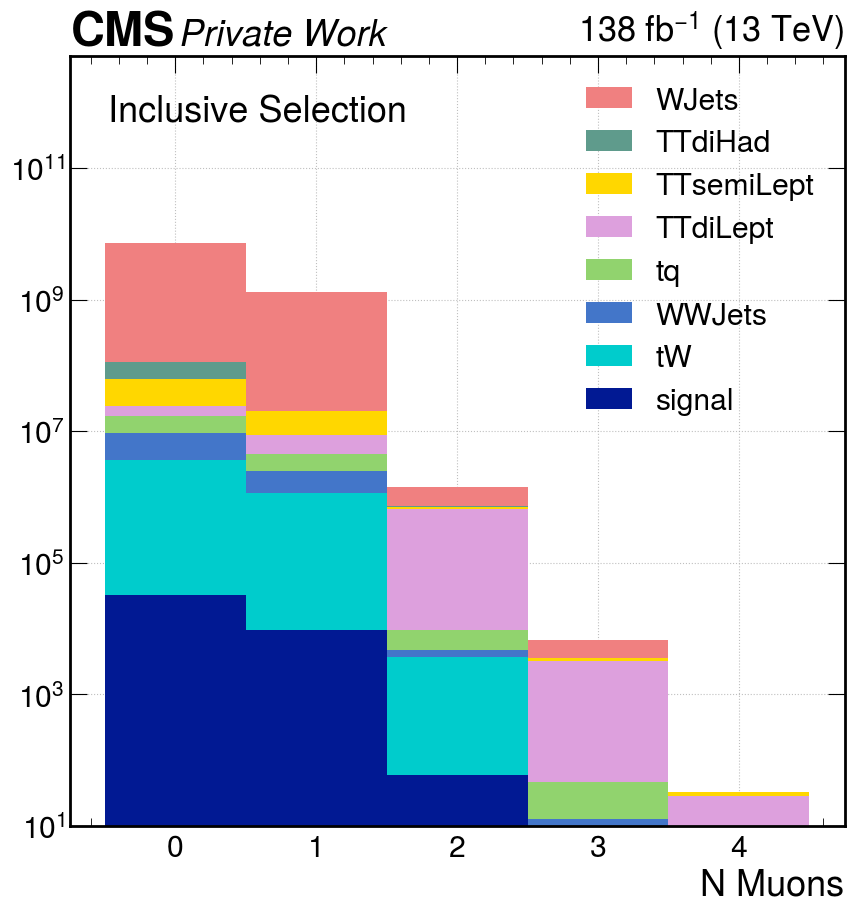
\includegraphics[width=1\linewidth]{fig//chap07-selection/nMuons.png}
            \caption{Distribution on the number of Muons per event.}
            \label{fig:n_mu}
        \end{figure}
\end{minipage}
\end{minipage}


\newpage
\subsection{Electrons}
The selection of electron candidates follows the same principles as the muon selections.
They are required to be into the tracker coverage $|\eta|<2.4$ and its momentum has to be $p_T>30 \GeV$.\\
\\
The identification and isolation of the electron are based on the \emph{medium} working point of \textit{Fall17IsoV2} \cite{2018ElectronConference}, a BDT model which assigns a score to the identification and isolation of the electron, taking as input informations about tracks, calo-clusters, shower shape, the amount of collinear radiation to the electron track, and the PF isolation.\\
\\
The MVA ID is trained on DrellYan+Jets MC samples, with prompt electrons as signal and unmatched plus non-prompt electrons as background, ignoring electrons from tau decays.\\
\\
The medium working point has an overall signal efficiency of $\sim 90\%$ and a background rejection efficiency $>98.5\%$.\\
\begin{minipage}{\linewidth}
    \begin{minipage}{0.53\linewidth}
        \begin{figure}[H]
            \centering
            \includegraphics[width=1\linewidth]{fig//chap07-selection/nElectrons.png}
            \caption{Distribution on the number of Electrons per event.}
            \label{fig:n_ele}
        \end{figure}
    \end{minipage}
    \hfill
    \begin{minipage}{0.46\linewidth}
        \vspace{-1.5cm}
        \begin{table}[H]
            \centering
            %\fontsize{13pt}{13pt}\selectfont
            \renewcommand{\arraystretch}{1.48}
            \begin{tabular}{c|c}
                \toprule
                \multicolumn{2}{c}{\textbf{Electrons}}\\
                \midrule
                \midrule
                $\mathbf{p_T}$& $>30 \GeV$\\
                \midrule
                $\bm{|\eta|}$& $<2.4$ \\
                \midrule
                \textbf{$e$ Identification}&Medium WP\\
                \textbf{+ Isolation}&Fall17IsoV2 \\
                &$(\epsilon \sim 90\%)$\\
                \bottomrule
            \end{tabular}
            \caption{Electrons selection cuts.}
        \end{table}      
    \end{minipage}
\end{minipage}


\subsection{Jets}\label{sec:jet}
The jets taken into consideration are the PF AK4 Jet candidates in the calorimeter coverage $|\eta|<4.8$ and with $p_T>20\GeV$.


\paragraph*{Identification}
The jet identification is based on the \emph{Tight jetID} that imposes different requirements on the composition of the jets in different $|\eta|$ regions.\\
The requirements are listed in Tab.\ref{tab:jet_id}

\begin{table}[H]
    \centering
    \fontsize{11pt}{11pt}\selectfont
    \begin{tabular}{l|c|c|c|c}
        \toprule
         \multicolumn{1}{c|}{$\bm{|\eta|\in}$}&  $[0,2.6]$& $[2.6,2.7]$ & $[2.7,3.0]$ & $[3.0,5.0]$\\
         \midrule
         \textbf{Neutral Hadron Fraction} & $<0.90$ &  $<0.90$ & - & $>0.20$\\
         \midrule
         \textbf{Neutral EM Fraction} & $<0.90$ & $<0.99$ & $\in[0.02,99]$ & $<0.90$\\
         \midrule
         \textbf{Number of Constituents } & $>1$ & - & - &  -\\
         \midrule
         \textbf{Charged Hadron Fraction} & $>0$ & - & - & -\\
         \midrule
         \textbf{Charged Multiplicity} & $>0$ & $>0$ & - & -\\
         \midrule
         \textbf{Number of Neutral Particles}& - & - & $>2$ & $>10$\\
         \bottomrule
    \end{tabular}
    \caption{Tight jet identification requirements.}
    \label{tab:jet_id}
\end{table}
The efficiency of the tight Id working point is $\epsilon>99\%$, whereas the background rejection is $>98\%$. 
\paragraph*{Cross-cleaning} 
Since the leptons are included in the jet clustering process, to avoid considering the leading lepton as an additional jet, a simple $\Delta R$ matching is performed. If the jet axis and the leading lepton are separated less than $\Delta R<0.4$, the jet is removed. 

\paragraph*{Pile-up rejection}
The identification of jets from pile-up relies on three types of properties of the jets:
\begin{itemize}
    \item  In the tracker acceptance, the tracks associated with the jets can be used to match the jet with the primary interaction vertex.
    \item The shape of the calorimetric deposit is different in case of overlap of multiple interactions.
    \item The objects' multiplicity.
\end{itemize}


\begin{minipage}{\linewidth}
    \begin{minipage}{0.35\linewidth}
    
        The identification of jets from pile-up is done exploiting the \emph{Jet puId},
        a BDT model score \cite{CMSCollaboration2020PileupData}. Its inputs are listed in Tab \ref{tab:puId_inputs}.\\
        \\
        This BDT is trained on DrellYan+Jets MC samples with jets of $p_T<50\GeV$, where there is the highest composition of PU jets.\\
        
    \end{minipage}
    \hfill
    \begin{minipage}{0.625\linewidth}
    \vspace{-1.65cm}
    \begin{figure}[H]
        \centering
        \includegraphics[width=\linewidth]{fig//chap07-selection/puid_bdt.png}
        \captionof{table}{PuID BDT input variables \cite{CMSCollaboration2020PileupData}.}
        \label{tab:puId_inputs}
    \end{figure}
        \vspace{0.1cm}
    \end{minipage}
\end{minipage}
The chosen working point is the \emph{Loose puId}, which corresponds to 99\%  efficiency for prompt jets with $|\eta| < 2.5$ and 95\% efficiency for prompt jets with $|\eta| > 2.5$.
\paragraph*{Jet energy scale corrections}
To allow a proper mapping of the energy of the reconstructed jet to the truth particle-level jet energy, a set of jet energy corrections is applied.\\
\\
In CMS, the jet energy scale corrections are separated into different steps applied sequentially and in a fixed order.\\
Each correction takes care of a different effect and consists of a rescaling of the jet four-vector \cite{2021Jet13TeV}.

\begin{figure}[H]
    \centering
    \includegraphics[width=\linewidth]{fig//chap07-selection/JEC_upscayl_2x_ultramix_balanced.png}
    \caption{Jet energy scale correction chain.}
    \label{fig:jerc}
\end{figure}
\begin{enumerate}
    \item \textbf{L1 Pile-Up}: remove the energy coming from pileup events, removing any dependence on the luminosity.\\
    The pileup corrections are determined from simulated QCD dijet events with and without pileup overlay.
    \item \textbf{L2L3 MC-truth corrections}: this correction has the scope to improve the accordance between the reconstructed jet energy and the particle-level energy, and to make the response of the jet energy uniform in $p_T$ and $\eta$. The related scale factors are evaluated on QCD dijet samples.
\end{enumerate}
The pile-up and MC-truth corrections are applied both on MC and data, while additional residual corrections are applied only on data: they are meant to correct differences of the order of 1\% within jet response in data and MC.

A summary of the jet energy corrections chain is shown in \Fig{fig:jerc}.

\paragraph*{Jet energy resolution corrections}\label{par:JERC}
The jet momentum resolution is different in the data with respect to the simulation. To replicate the resolution observed in the data, the jets' four vectors are rescaled in a procedure called \emph{smearing} \cite{2021Jet13TeV}:\\
if a reconstructed jet and a jet at the generator level (GenJet) are matched through the relation $\Delta R(\text{Jet,GenJet})<0.2$ and $|p_T-p_T^{\text{Gen}}|<3\sigma p_T$, the jet four-vector is scaled by a factor
\begin{equation}
    f=1+\textit{SF}\:\frac{p_T-p_T^{\text{Gen}}}{p_T}
\end{equation}
where $\sigma$ is the jet energy resolution measured with data, and SF is the scale factors that depend on the $\eta$ region in which the jet belongs.
Otherwise, if there is not any match between the jet and the genjets, a random Gaussian smearing is applied.


\paragraph*{Flavor tagging corrections}\label{par:tag_corr}
The distribution shapes of the \DeepJet discriminators are another element that shows discrepancies between data and simulated samples.\\
To address this problem the events are reweighted:
a weight is applied to each selected jet and an event weight is defined as the product of all the jet weights inside the event.\\
The event weights obtained from these corrections are then multiplied by the event weights provided by the generator program, as already explained in sec. \ref{sec:MC}. 
\\
\\
In this work, the applied corrections are the ones related to the b tagging and to the c tagging.\\
These scale factors are computed through an iterative tag-and-probe procedure \cite{2021B-tagging2018.}, in different bins of $\eta$,$p_T$, and \DeepJet score to compute simultaneously SF for both heavy and light flavor jets.
\begin{itemize}
    \item For heavy-flavor jets, dileptonic $\ttbar$ events are exploited, using one b jet that passes the medium working point as a tag and the second b jet as a probe.
    \item For light jets, Z+jets dileptonic samples are used, using a b tag loose working point as a veto to select the tag jet.
\end{itemize}
The procedure to obtain SFs related to the c-tagging is similar, using W+c samples, but for them, the binning depends both on the CvB and CvL discriminators defined as
\begin{equation}
\begin{aligned}
     \text{CvL} &= \frac{P(c)}{P(c) + P(udsg)}\\
     \text{CvB} &= \frac{P(c)}{P(c) + P(b)} \cdot P(b) 
\end{aligned}
\end{equation}
where $P(b), P(c),$ and $P(udsg)$ are the b,c, and light flavor \DeepJet scores.



\begin{minipage}{\linewidth}
\begin{minipage}{0.53\linewidth}
      \begin{figure}[H]
            \centering
            \includegraphics[width=1\linewidth]{fig//chap07-selection/nJet.png}
            \caption{Distribution on the number of Jets per event.}
            \label{fig:n_jet}
        \end{figure}
\end{minipage}
\hfill
\begin{minipage}{0.46\linewidth}
\vspace{-1.25cm}
\begin{table}[H]
    \centering
    \begin{tabular}{c|c}
        \toprule
        \multicolumn{2}{c}{\textbf{Jets}}\\
        \midrule
        \midrule
        
        $\mathbf{p_T}$& $>20 \GeV$\\
        \midrule
        $\bm{|\eta|}$& $<4.8$ \\
        \midrule
        \textbf{Identification} & Tight\\
        \midrule
        \multirow{2}{*}{\textbf{Isolation}} & Lead. Lept. \\
        &$\Delta R>0.4$ matching\\
        \midrule
        \textbf{Pile-up Id} & Loose  $(\epsilon\sim99\%)$ \\
        \bottomrule
    \end{tabular}
    \caption{Jets selection cuts.}
\end{table}
\end{minipage}   
\end{minipage}

 
\newpage
\section{Event selections}
As already discussed, the chosen event selection is minimal to avoid large losses in signal acceptance efficiency.\\ 
The signal events are targeted in two different final states, defined by the flavor of the lepton used as a probe, so after the physics objects selection and the requirement of the presence of at least 4 jets, two different channels are defined: a Muon channel that contains events with at least one selected muon, and an Electron channel that contains events with at least one selected electron.

\vspace{1.25cm}
\begin{figure}[H]
     \centering
     \begin{subfigure}{0.42\linewidth}
         \includegraphics[width=\linewidth]{fig//chap07-selection/selection/Leading_Electron_pt.png}
         \caption{Leading electron}
     \end{subfigure}
     \begin{subfigure}{0.42\linewidth}
        \includegraphics[width=\linewidth]{fig//chap07-selection/selection/Leading_Muon_pt.png}
         \caption{Leading muon}
     \end{subfigure}
     \begin{subfigure}{0.42\linewidth}
        \includegraphics[width=\linewidth]{fig//chap07-selection/selection/Leading_Jet_pt.png}
         \caption{Leading Jet}
     \end{subfigure}
    \begin{subfigure}{0.42\linewidth}
        \includegraphics[width=\linewidth]{fig//chap07-selection/selection/Second_Leading_Jet_pt.png}
         \caption{Second Leading Jet}
     \end{subfigure}
\end{figure}
\vspace{-0.5cm}
\begin{figure}[H]
    \ContinuedFloat
    \centering
    \begin{subfigure}{0.42\linewidth}
        \includegraphics[width=\linewidth]{fig//chap07-selection/selection/Third_Leading_Jet_pt.png}
         \caption{Third Leading Jet}
     \end{subfigure}
    \begin{subfigure}{0.42\linewidth}
        \includegraphics[width=\linewidth]{fig//chap07-selection/selection/Fourth_Leading_Jet_pt.png}
         \caption{Fourth Leading Jet}
     \end{subfigure}
        \caption{$p_T$ distributions after the object selection and the $1e/\mu$ + 4 jets requirements.}
\end{figure}
\vspace{-0.5cm}
An additional selection on the most b-tagged jet is imposed using the medium working point.\\
The cumulative efficiencies of each cut are described in Tab.\ref{tab:event_selection} and the final event counts normalized with the RunII luminosity and the respective cross-sections in \Fig{fig:event_selection}
\begin{table}[H]
    \centering
    \fontsize{11.pt}{11.pt}\selectfont
    \begin{tabular}{l|ccc||ccc}
        \toprule
         &  \multicolumn{3}{c||}{\textbf{Muons}} &\multicolumn{3}{c}{\textbf{Electrons}} \\
         \midrule
         \midrule
         Cumulative& \multirow{2}{*}{$\bm{\geq1 \mu}$} & \multirow{2}{*}{$\bm{\geq4}$ \textbf{Jets}} & $\bm{\max({\textbf{btag}})}$& \multirow{2}{*}{$\bm{\geq1e}$} & \multirow{2}{*}{$\bm{\geq4}$ \textbf{Jets}} & $\bm{\max({\textbf{btag}})}$\\
         efficiencies&&&$\bm{>0.27}$&&&$\bm{>0.27}$\\
         \midrule
         \textbf{signalMu}& $64.1\%$ & $53.5\%$ & $51.8\%$ &0.22\% & 0.18\% & 0.16\%\\
         \midrule
         \textbf{signalEle}& 0.65\% & 0.50\% & 0.46\% & 52.3\% & 43.5\% & 42.1\% \\
         \midrule
         \textbf{signalTau}& 4.86\% & 3.95\% & 3.80\% & 3.37\% & 2.79\% & 2.70\%\\
         \midrule
         \textbf{TTsemiLeptMu}& 63.6\% & 54.0\% & 49.8\% & 0.15\% & 0.12\% & 0.09\% \\
         \midrule
         \textbf{TTsemiLeptEle}& 0.48\% & 0.39\% & 0.30\% & 51.9\% & 45.6\% & 41.7\% \\
         \midrule
         \textbf{TTsemiLeptTau}&4.59\%  & 3.84\% & 3.48\% &3.24\% &2.82\% &2.58\%\\
         \midrule
         \textbf{TTdiLept}& 40.9\% & 27.4\% & 25.3\% & 33.8\% &22.7\% &20.9\% \\
         \midrule
         \textbf{TTdiHad}& 0.45\%  & 0.40\% & 0.31\% & 0.16\% &0.15\% &0.12\% \\
         \midrule
         \textbf{WJets Lept}& 15.0\% & 0.24\% & 0.03\% & 10.6\% & 0.20\% &0.03\%\\
         \midrule
         \textbf{WWJets SL}& 19.5\% & 5.53\% & 0.79\% & 15.3\% & 4.42\% & 0.64\% \\
         \midrule
         \textbf{tW SL}& 23.6\% & 13.6\%  & 11.3\% & 19.0\% &10.9\% &9.11\%  \\
         \midrule
         \textbf{tq Lept}& 21.6\%  &6.23\% & 5.42\% & 15.1\% & 4.40\% &3.81\% \\
         \bottomrule
    \end{tabular}
    \caption{Cumulative efficiencies of the selections in the Muons and Electrons channel after the physics objects selection}
    \label{tab:event_selection}
\end{table}
\vspace{-0.5cm}
The main background contribution in each channel is from the \ttbar semileptonic decay, which is 3 orders of magnitude greater than the signal.
Another significant contribution is from the \ttbar dileptonic (DL) process. The contribution from the WW+Jets process is two orders of magnitude smaller than \ttbar SL and \ttbar DL processes, while the remaining processes' contribution is one order of magnitude smaller than the leading backgrounds. 

\begin{figure}[H]
     \centering
     \begin{subfigure}{0.42\linewidth}
         \includegraphics[width=\linewidth]{fig//chap07-selection/btag/Max_DeepJetB.png}
         \caption{Max \DeepJet B}
     \end{subfigure}
    \begin{subfigure}{0.42\linewidth}
         \includegraphics[width=\linewidth]{fig//chap07-selection/btag/Second_Max_DeepJetB.png}
         \caption{Second Max \DeepJet B}
     \end{subfigure}
    \begin{subfigure}{0.42\linewidth}
         \includegraphics[width=\linewidth]{fig//chap07-selection/btag/Third_Max_DeepJetB.png}
         \caption{Third Max \DeepJet B}
     \end{subfigure}
    \begin{subfigure}{0.42\linewidth}
         \includegraphics[width=\linewidth]{fig//chap07-selection/btag/Fourth_Max_DeepJetB.png}
         \caption{Fourth Max \DeepJet B}
     \end{subfigure}
          \begin{subfigure}{0.42\linewidth}
         \includegraphics[width=\linewidth]{fig//chap07-selection/btag/Max_DeepJetC.png}
         \caption{Max \DeepJet C}
     \end{subfigure}
    \begin{subfigure}{0.42\linewidth}
         \includegraphics[width=\linewidth]{fig//chap07-selection/btag/Second_Max_DeepJetC.png}
         \caption{Second Max \DeepJet C}
     \end{subfigure}
     \caption{B-tag and c-tag score distributions after the object selection and the 1 lepton + 4 jets requirements.}

\end{figure}
\begin{figure}[H]
     \centering
     \begin{subfigure}[t]{\linewidth}
         \centering
         \includegraphics[width=\linewidth]{fig//chap07-selection/ele_selection.png}
         \caption{\textbf{Electrons channel}}

     \end{subfigure}
     
     \vspace{1cm}
     \begin{subfigure}[b]{\linewidth}
         \centering
        \includegraphics[width=\linewidth]{fig//chap07-selection/mu_selection.png}
         \caption{\textbf{Muons channel}}
     \end{subfigure}
     \vspace{0.5cm}
        \caption{Event number for each process for each cut. In the legend the final number of events for each process after the preselection is shown. The processes are ordered in their final event number.}
        \label{fig:event_selection}
\end{figure}
\newpage
\section{Neutrino reconstruction}\label{sec:nu_reco}
To fully reconstruct the kinematics of the event and to allow the reconstruction of the leptoninc decaying top quark, the longitudinal component of the neutrino was reconstructed exploiting the transverse momentum of the missing energy, its pseudorapidity, the lepton's four vector, and fixing the mass of the \PW boson to $m_W=80.385 \GeV$.
\begin{equation}
    (p^\mu_\nu+p^\mu_\ell)^2=m_W^2 
\end{equation}
The equation to solve for $p_z^{\nu}$ is a second order equation
\begin{equation*}
    p_z^\nu=\dfrac{p_z^\ell(m_W^2+2\vec{p}_T^{\:\ell} \cdot \vec{p}_T^{\:\nu})\pm\sqrt{(p_z^\ell)^2 (m_W^2+2\vec{p}_T^{\:\ell} \cdot \vec{p}_T^{\:\nu})^2-|p_T^\ell|^2[4(E_\ell p_T^\nu)^2-(m_W^2+2\vec{p}_T^{\:\ell} \cdot \vec{p}_T^{\:\ell})^2)]}}{2|p_T^\nu|^2}
\end{equation*}

The equation has two solutions, that can also be complex. If the equation has a complex solution the real part is taken but, if the equation allows two real solutions, we must choose one of them.\\
In \Fig{fig:nu_comparison} it is shown a comparison between the solution with the smaller magnitude, the solution with the greater magnitude, and the truth value of $p_z^\nu$ at the LHE level.\\
This study was performed using signal samples.


\begin{figure}[H]
    \centering
    \includegraphics[width=1\linewidth]{fig//chap07-selection/Pznu_LHE_comparison.png}
    \caption{In the left panels there are the events that have two real solutions, while in the right panels the ones with the complex solutions of which only the real part is shown. In the top panel the distribution of the absolute value of the solutions and the LHE truth value are shown, while in the bottom panels, there are the distributions of the differences between the solutions and the LHE truth values. The $\Delta$ in the legend is the discriminant of the second-order equation. The distributions are in arbitrary units.}
    \label{fig:nu_comparison}
\end{figure}




The distribution of the solutions with the smaller absolute value is in better accordance with the truth value, so the strategy will be:\\
\begin{minipage}{\linewidth}
    \begin{minipage}{0.42\linewidth}

\begin{itemize}
    \item The solutions are complex: take the real part.
    \item There are two real solutions: take the smallest in the absolute value.
\end{itemize}

        Of course, in the complex solution case, if we consider only the real part, the chosen value will violate the W mass constraint, so, the invariant mass of the sum of the lepton and the reconstructed neutrino will not be $m_W$. In  \Fig{fig:LeptW_reco} the distribution of the leptonic W mass is shown.
    \end{minipage}
    \hfill
    \begin{minipage}{0.55\linewidth}
    \vspace{-0.2cm}
    \begin{figure}[H]
    \centering
    \includegraphics[width=\linewidth]{fig//chap07-selection/Wmass_reconstructed.png}
    \caption{Distribution of the reconstructed W mass in the real solution case and the complex solution case, taking only the real part.}
    \label{fig:LeptW_reco}
\end{figure}
        
    \end{minipage}

\end{minipage}

\newpage
\
\newpage
%!TEX root = ../thesis.tex
\newchap{Signal reconstruction and interpretation}\label{sec:kin}
\vspace{-1cm}
\minitoc
\vspace{0.5cm}
This chapter focuses on the kinematical reconstruction and interpretation of the signal events tackling the jet-parton assignment problem.
\\
\\
The jet-parton assignment is first done with just one jet, the one b-jet associated with the decay of the top quark that decays into the W boson that decays leptonically. This simplified benchmark is used to perform a feature ranking exploiting the N+1, N-1 method and to select the best model that will be used in the full jet-paron assignment.

\section{Jet-parton assignment}
The Jet-Parton assignment task consists of associating at each of the four quark partons a Jet to fully reconstruct the topology and the kinematics of the event.\\
\\
This is a difficult task due to the combinatorial nature of the problem: If there are N jets in an event, the total number of combinations in which is possible to assign a jet to the 4 partons is $N!/(N-4)!$, so, for example, if an event has 10 jets, there are more than 5000 possible combinations.\\
\\
Usually, this task is accomplished through a kinematic fit that consists of finding the combination of jets for each event that minimizes the chi-square of all the invariant masses\footnote{The $\chi^2$ can also include terms related to the flavor tagging like $[(b_{j_1}-1)^2+(c_{j_2}-1)^2+(b_{j_3}-1)^2+(b_{j_4}-1)^2]/\sigma^2$ where $b_{j_i},c_{j_i}$ are the b and c tag score of the i-th jet and $\sigma$ a hyperparameter. NB: non è un vero iperparametro e in questo modo chi2 NON funziona, errore sugli score non gaussiani (neanche simmetrici).E' una cosa empirica pezzente}.
\begin{equation}
    \chi^2=\frac{(m_{j_1j_2}^{\text{inv.}}-m_W)^2}{\Gamma^2_W}+\frac{(m_{j_1j_2j_3}^{\text{inv.}}-m_t)^2}{\Gamma^2_t}+\frac{(m_{j_4\ell\nu}^{\text{inv.}}-m_t)^2}{\Gamma^2_t}
\end{equation}
This is an unsupervised approach but in this work another approach is used, exploiting supervised multivariate models like neural networks that allow us to exploit not only the kinematic variables of jets but also their flavor score and the correlations between all the observables.

\subsection{Leptonic bJet benchmark}

\subsubsection*{Event level features}
\subsubsection*{{$N-1,N+1$} ranking}
\subsubsection*{Object level features}
\subsection{Full Jet-parton assignment}


%%!TEX root = ../thesis.tex
\newchap{Event classification and signal extraction}\label{sec:signal}
\vspace{-1cm}
\minitoc
This chapter is focused on the signal-background discrimination. It will begin by demonstrating a basic one-dimensional feature ranking. Subsequently, JPANet will be adapted to tackle the signal-background discrimination challenge, and its score will be employed to execute a template fitting procedure on both the Muon and Electron channels, utilizing the Asimov dataset.
Once the statistical uncertainties associated with the $\PW \to cb$ rate are determined, we will also introduce and assess the systematic uncertainties and their impact on the signal rate extraction.
\begin{minipage}[H]{\linewidth}
\begin{minipage}{0.35\linewidth}
        \centering
        \includegraphics[height=0.7\textheight]{fig//chap08-kin_reco/ranking1D.png}
        
\end{minipage}
\hfill
\begin{minipage}{0.62\linewidth}
\vspace{-1cm}
\section{Unidimensional feature ranking}
To begin,  we can once again employ the metric $d$ to evaluate and rank the observables that discriminate the signal from the background.\\
\\
In this context, $d$ is computed between the signal and the $\ttbar$ semileptonic process, which is the primary source of background.\\
\\
All observables are treated as flattened, meaning that all objects within the events are combined in the same histograms, disregarding the event's inherent structure.\\
\\
The ranking process is carried out within the Muon channel following the initial preselection.\\
The results of this one-dimensional ranking are depicted in \Fig{fig:1Drank}.\\
\\
Notably, the observables with the highest ranking are those associated with b-tagging, exhibiting $d$ values of approximately 0.1.\\
Other observables produce results that are about an order of magnitude smaller, and the latests are due mostly to statistical fluctuations.

\end{minipage}
        \label{fig:1Drank}  
        \captionof{figure}{Unidimensional feature ranking using the metric $d$ between flattened signal observables and \ttbar semileptonic observables }
\end{minipage}
\section{Event classification}
\subsubsection*{SBANet} Since we have already demonstrated the ability of JPANet to reconstruct and interpret the signal events, we can exploit the same model to tackle the signal-background discrimination task.\\
To achieve this, we simply need to make some adjustments to JPANet, creating another network which will be denoted as "Signal-Background Attention Network" (SBANet).\\
The training and evaluation of this network will be conducted independently for the Muon and Electron channels.
\\
The differences between SBANet and JPANet are:\\
\\
\textbf{Jet Inputs}: In SBANet, all three \DeepJet scores are added to the Jet head (b-tag,CvB,CvL).
\\
\\
\textbf{Hyper-parameters}: After experimenting with various configurations, we found that the network required increased complexity. This entailed raising the number of units in each feed-forward layer to 128 and adjusting the dropout probability to 2\%.
\\
\\
\textbf{Self-attention pooling}: The JPANet's output initially produces a 7x4 matrix, as it assigns scores to pairs of jet-partons. However, we need to derive a single score for the entire event. To accomplish this, we condensed the physics objects embedding sequence into a single dimension using a self-attention pooling layer. This layer assigns weights to each element of the sequence (i.e., the physics objects) based on attention scores and computes a weighted average across the sequence. Subsequently, we introduced three additional feed-forward layers.
\\
\\
\textbf{Event self-attention}: We aimed to have the self-attention pooling calculate attention scores over all physics objects, not just the jets. Consequently, we transformed JPANet's cross-attention into a self-attention mechanism covering the concatenated sequence of jets and the leptonic W.
\\
\\
\textbf{Output layer} The output of SBANet is a 3-dimensional layer equipped with the softmax function. Three classes are defined: the signal, the $\ttbar$ semileptonic process, and the $\ttbar$ dileptonic process. This enables the network to better distinguish the signal from the two primary sources of background, even though, ultimately, we only consider the signal score.
\\  
\\
\textbf{Secondary leptons head} 
To enhance SBANet's ability to identify di-leptonic events, we introduced an additional head. In the muon(electron) channel, this head comprises a sequence of three elements: the second leading muon(electron), the leading and the second leading electron(muon).
The lepton features are limited to kinematic variables $(p_T,\eta,\phi)$, and the head is linked to a 2-layer feed-forward neural network.\\
The sequence of secondary leptons' embeddings is then combined with the complete event sequence before the self-attention pooling layer.
\\
\\
\textbf{Invariant mass heads and pair-wise attention biases} The two self-attention layers in the network were modified to include pair-wise physics object features, such as invariant masses.
Let's recall what is the scaled dot product:
\begin{equation}
    \text{Softmax}\left( \frac{QK}{\sqrt{d_k}} \right)V
\end{equation}
The product $QK$ is a $N\times N$ matrix where N is the length of the sequence.\\
Given that we can include the invariant masses of couples of physics objects by just adding a term in the softmax function
\begin{equation}
    \text{Softmax}\left( \frac{QK+\hat{M}}{\sqrt{d_k}} \right)V
\end{equation}
where $\hat{M}$ is a linear embedding of the matrix $M$ that contains all the invariant masses
\begin{equation}
\begin{aligned}
    M_{ij}&=\sqrt{(p_i+p_j)^\mu(p_i+p_j)_\mu} & \text{if } i\neq j\\
    M_{ij}&=m_i & \text{if } i=j\\
\end{aligned}
\end{equation}
The M matrix is symmetric and has $N(N+1)/2$ independent components.\\
\\
The strategy to implement this in SBANet is adding another input head containing for each event a vector of length 36 with the square invariant masses of the couple of jets and the leptonic W.
\begin{equation*}
    \text{Mass head inputs}=\Biggl[ \dboxed{m_W,m_{Wj_1},\:\dots\:,m_{Wj_7},\dboxed{m_{j_1},m_{j_1 j_2},\:\dots\:,m_{j_6},m_{j_6 j_7},m_{j_7}}}\: \Biggr]
\end{equation*}
This vector contains all the independent components of the M matrix.\\
Given the presence of significant outliers in the invariant masses, they are transformed with the function $\log(1+m)$ and then normalized with a batch norm layer.\\
There are two attention layers in SBANet: the first is a self-attention layer that works only on the jet sequence, while the second works on the jet + leptonic W sequence, so we have to build two different mass embeddings.\\
\\
For the first jet self-attention, only the mass inputs that are not related to the leptonic W boson are considered. They are 28 elements that are fed to a 4-layer feed-forward neural network of size [28,128,128,28]. This network that has the same number of neurons in the first and the last layer is called Autoencoder.\\
The 28 output elements of the autoencoder are used to build the full $7\times 7$ M matrix that will be used as attention bias in the jet self-attention.\\
The same thing is done with the second event self-attention but considering all the mass head inputs and, in this case, the autoencoder size will be [36,128,128,36]\\


\begin{minipage}{\linewidth}
    \begin{minipage}{0.52\linewidth}
        \paragraph*{Training and evaluation}
        The network is trained and evaluated separately in the Muon and Electron channels. The dataset is divided into 85\% training and 15\% validation and is illustrated in \Tab{tab:SBANet_dataset}. \footnotemark\\
        To take into account the imbalance between the three classes, the cross-entropy loss function of SBANet is reweighted.
    \end{minipage}
    \hfill
    \begin{minipage}{0.45\linewidth}
        \centering
        \begin{tabular}{l|c|c}
            \toprule
             & \textbf{Training} & \textbf{Validation}\\
            \midrule
             signal& $9.1 \cdot 10^6$  & $1.6 \cdot 10^6$\\
             TTSL & $1.0 \cdot 10^8$ & $1.8 \cdot 10^7$\\
             TTDL & $2.0\cdot 10^7$ & $3.5 \cdot 10^6$\\
        \end{tabular}
        \captionof{table}{SBANet train and validation datasets before the Muon/Electron channel preselection.}
        \label{tab:SBANet_dataset} 
    \end{minipage}
\end{minipage}
\footnotetext{These events are not included in the effective MC luminosity shown in \Tab{tab:samples}. These are additional events used only to train and validate the network}\\
The loss functions are shown in \Fig{fig:SBANET_loss} and don't show any sign of overfitting.


\begin{figure}[H]
    \centering
    \includegraphics[height=0.805\textheight]{fig//chap09-sigback/SBANet.png}
    %\caption{SBANet}
    \label{fig:SBANet}
\end{figure}

\begin{minipage}{0.58\linewidth}
\begin{table}[H]
    \centering
    \fontsize{11.8pt}{11.8pt}\selectfont
    \begin{tabular}{l|l}
    \toprule
        \textbf{Head} & \textbf{Input features} \\
    \midrule
         Jets & $[p_T,\eta,\phi,\text{bTag},\text{CvB},\text{CvL}]$ \\
         \midrule
         LeptW & $[p_T^\ell,\eta^\ell,\phi^\ell,p_T^\nu,\eta^\nu,\phi^\nu]$\\
         \midrule
         Sec. Lept.& $[p_T,\eta,\phi]$ \\
         \midrule
         Masses & 36 Jets+LeptW inv. masses\\
         \bottomrule
    \end{tabular}
    %\caption{Caption}
    \label{tab:sbanet_inputs}
\end{table}
\end{minipage}
\hfill
\begin{minipage}{0.4\linewidth}
    \begin{table}[H]
    \centering
    \begin{tabular}{l|l}
    \toprule
        Act. function & Swish\\
        Loss& Cross-Entropy\\
        Optimizer & RAdam \\
        Learn. rate & 0.001\\
        Batch size & 20000\\
        Dropout  & 0.02\\  
        \bottomrule
    \end{tabular}
\end{table}
\end{minipage}
\captionof{figure}{SBANet schematics, inputs, and hyper-parameters.}

\begin{figure}[H]
    \centering
    \includegraphics[height=0.48\textheight]{fig//chap09-sigback/loss_Muon.png}
    \includegraphics[height=0.48\textheight]{fig//chap09-sigback/loss_Electron.png}
    \caption{SBANet training and validation loss for the muon and electron channel.}
    \label{fig:SBANET_loss}
\end{figure}


\begin{figure}[H]
    \centering
    \includegraphics[height=0.48\textheight]{fig//chap09-sigback/stack_score_muons.png}
    \includegraphics[height=0.48\textheight]{fig//chap09-sigback/stack_score_electrons.png}
    \caption{Stacked distribution of the SBANet scores for each process and signal sensitivity ($\bm{Q}$) plot in the muon (top) and electron (bottom) channel.}
    \label{fig:SBANET_scores}
\end{figure}

\section{$|V_{cb}|^2$ extraction}
To extract the $|V_{cb}|^2$ rate, the SBANet score is employed to perform a template fit.

\begin{minipage}{\linewidth}
\begin{minipage}{0.43\linewidth}
\begin{table}[H]
    \centering
    \begin{tabular}{l|cc}
    \toprule
        \textbf{Channel} & $\bm{Q}$ & $\dfrac{\bm{\sigma[R(W \to cb)]}}{\bm{R(W \to cb)}}$ \\
        \midrule
         Muon & 98.50 & 10.1\%\\
         Electron & 68.65 &  11.3\%\\
         Combined & 177.15 & 7.5\%\\
         \bottomrule
    \end{tabular}
    \caption{signal sensitivity and estimate of the statistical uncertainties on $|V_{cb}|^2$ for each channel.}
    \label{tab:stat_unc}
\end{table}
    
\end{minipage}
\hfill
\begin{minipage}{0.52\linewidth}
    To expand the region with the highest signal purity, the scores are transformed with the inverse hyperbolic tangent function and then binned in such a way as to maximize the signal sensitivity, maintaining at least one event in each bin.
    Even before executing the fit, the statistical uncertainties on $|V_{cb}|^2$ can be estimated through the signal sensitivity.
\end{minipage}

    
\end{minipage}




\iffalse
\begin{equation*}
    \begin{aligned}
        Q&=98.5 &\implies \frac{\sigma[R(\PW \to cb)]}{R(\PW \to cb)}&\sim 10.1\% & (\text{Muon channel})\\
        Q&=44.1 &\implies \frac{\sigma[R(\PW \to cb)]}{R(\PW \to cb)}&\sim 15.0\% & (\text{Electron channel})\\
        Q&=142.6 &\implies \frac{\sigma[R(\PW \to cb)]}{R(\PW \to cb)}&\sim 8.4\% & (\text{Combined})\\
    \end{aligned}
\end{equation*}
\fi

\paragraph*{Template fit}
The statistical uncertainties on $|V_{cb}|^2$ are derived using the profile likelihood method using the Asimov dataset, as described in Sec. \ref{sec:profile}.\\
\\
The signal events in the histogram are normalized with the RunII luminosity
\begin{equation*}
    N_s=\mathcal{L}_{\text{RunII}}^I \times \epsilon_{\text{channel}}\times \sigma(\ttbar)\times \mathcal{BR}(\PW \to \ell \nu)\times (1-\mathcal{BR}(\PW \to \ell \nu)) \times \frac{|V_{cb}|^2}{2}
\end{equation*}
where $|V_{cb}|^2$ is the parameter of interest to fit, so the expectation value of the Poisson distributions in the likelihood will be
\begin{equation*}
    \lambda^{(b)}(|V_{cb}|^2) = |V_{cb}|^2 \cdot \dfrac{N_s^{(b)}}{\widetilde{|V_{cb}|^2}}+\sum_p^{\text{bkgs}} N_p^{(b)}
\end{equation*}
where $\widetilde{|V_{cb}|^2}$ is the value used to normalize the histograms and $N_p^{(b)}$ are the number of events for the process $p$ in the b-th bin.
The result of the fit is shown in \Fig{fig:stat_fit}


\subsection{Systematic uncertainties}

In this analysis, the most relevant systematic uncertainties are the following:

\begin{itemize}
    \item \textbf{b/c-tagging uncertanties} 
    The derivation of the b/c-tagging scale factors, described in Sec. \ref{par:tag_corr}, is subject to different systematical uncertainties \cite{Sirunyan_2018}. 
    
    \iffalse
    The primary sources are the following:
    \begin{itemize}
        \item[\ding{111}] \textit{Sample purity}: The purity of the samples used to compute the light flavor SFs can be compromised by the contamination of heavy flavor jets associated with the Z boson, while for the heavy flavor SFs, the contamination of light jets in the $\ttbar$ sample can occur due to the production of additional partons.\\
        To take into account the uncertainties on the contamination, the rate of $\ttbar$ events produced in association with two or more additional partons and the fraction of heavy flavor jets in the Z+Jets samples are varied of $\pm 20\%$
        
        \item[\ding{111}] \textit{Statistical uncertainties} This source accounts for the statistical fluctuations in different SFs bins that affect the more low-populated regions like the ones with high values of b-tag score

        

        \iffalse
        \item[\ding{111}] \textit{Theoretical MC uncertainties} Uncertainties related to the parameter of the generator like the renormalization scale and the parton shower settings
        \fi
    \end{itemize}
    \fi
    \item \textbf{JES/JER} Uncertainties related to the jet energy scale and resolution corrections described in Sec. \ref{par:JERC}.

    \item \textbf{Luminosity} Uncertainties on the RunII luminosity: 1.6\%
    \item \textbf{Channel acceptance} Uncertainties on the acceptance of each signal region: 1\%(2\%) Muon(Electron) channel.
    \item \textbf{$\ttbar$ cross-section} Uncertainties on the $\ttbar$ cross-section: 5\%
\end{itemize}
The impact of the systematic uncertainties is evaluated using the profile likelihood method with normal priors for each nuisance and is shown in \Tab{tab:res}.


\begin{minipage}{\linewidth}
    \begin{minipage}{0.74\linewidth}
        \begin{figure}[H]
        \centering
        \includegraphics[width=\linewidth]{fig//chap09-sigback/stat_like.png}
        
        
        \end{figure}
    \end{minipage}
    \hfill
    \begin{minipage}{0.25\linewidth}
        
        \begin{table}[H]
            \centering
            \begin{tabular}{l|c}
                \toprule
                \multicolumn{2}{c}{\textbf{$|V_{cb}|^2$ Stat. Unc.}} \\
                \midrule
                 Muon & 9.0\% \\
                 Electron & 11.2\% \\
                 Combined & 7.0\% \\
                 \bottomrule
            \end{tabular}
            \label{tab:my_label}
        \end{table}
    \end{minipage}
    
    \captionof{figure}{Profile likelihood without nuisances on the SBANet score templates in the muon channel, electron channel, and combined.}
    \label{fig:stat_fit}
\end{minipage}


\begin{table}[H]
    \centering
    \begin{tabular}{l|c}
    \toprule
    \textbf{Uncertainties} & \textbf{Impact}\\
    \midrule
         Statistical   & 7\% \\
         \midrule
         b-tagging   & 7\% \\
         c-tagging   & 4\% \\
         JES/R   & 3\% \\
         Lumi+XSec+Acceptances  & 2\% \\
         \midrule
         Total   & 11\%\\
         \bottomrule
    \end{tabular}
    \caption{Impact of the systematic uncertainties and total uncertainties on the $|V_{cb}|^2$ determination.}
    \label{tab:res}
\end{table}

The uncertainties on $|V_{cb}|$ are half of those on $|V_{cb}|^2$, so the expected relative uncertainty on $|V_{cb}|$ is 5.5\% ($3.5\%$ Stat. + $4.4\%$ Syst.)
\begin{equation*}
    |V_{cb}|=0.041 \pm 0.002
\end{equation*}

 This relative uncertainty is already less than the 7\% tension shown by the $|V_{cb}|$ puzzle, but the systematical uncertainties can be further reduced by deriving $|V_{cb}|$ from the branching fractions ratio instead of from the signal rate, providing a great opportunity to address the $|V_{cb}|$ puzzle.\\


%%!TEX root = ../thesis.tex
\newchap{Conclusion}\label{sec:END}
\vspace{-1cm}
Currently, $|V_{cb}|$ is the CKM element measured with the largest relative uncertainties beside $|V_{ub}|$. Furthermore, the determination performed exploiting the semileptonic decays of B mesons exhibits a 7\% difference between the exclusive and the inclusive measurements, which leads to a $3\sigma$ tension.\\
\\
This thesis introduces a method to perform a direct measurement of $|V_{cb}|$ at LHC through the hadronic decays of $\PW$ bosons, exploiting the semileptonic decay of $\PW$ pairs to avoid the QCD background that would make an inclusive determination an impossible task.
\\
\\
The presented analysis focused on events where the \PW pairs are produced by di-top decays and where a \PW boson decays into a muon or electron and the other into a cb quark pair.\\
\\
To discriminate the signal from the background, cutting-edge machine-learning techniques were employed, in particular attention networks. 
A first attention network was built to address the signal interpretation optimization problem and then adapted to the signal-background discrimination task.\\
The network was trained separately on muon and electron signal regions and the output scores were employed to extract $|V_{cb}|$ through a template fit.\\
The fit was performed using the profile likelihood method, adding additional nuisance parameters to evaluate the systematic uncertainties on the b/c tagging and the jet energy scale/resolution.
Using the Asimov dataset, a combined relative statistical precision on $|V_{cb}|$ of $7.8\%$ ($3.5\%$ Stat. + $7\%$ Syst.) was obtained, which is comparable with the $7\%$ difference of the $|V_{cb}|$ puzzle.
\\
\\
In the end, the presented method is a promising prospect to tackle the $|V_{cb}|$ puzzle with a novel strategy, providing a new determination at the natural energy scale of the \PW boson which is also independent of non-perturbative QCD theoretical uncertainties.
On top of that, while in this work $|V_{cb}|$ was fitted directly as the parameter of interest, the determination could be further improved by deriving $|V_{cb}|$ from the ratio of branching fractions $|V_{cb}|^2=2\mathcal{BR}(\PW \to cb)/\mathcal{BR}(\PW \to qq)$, since it would allow cancellation in systematical uncertainties.

% REFERENCES
%!TEX root = ../thesis.tex

%%%%%%%%%%%%%%%%%%%%%%
%     References     %
%%%%%%%%%%%%%%%%%%%%%%

\message{^^J ^^J REFERENCES ^^J ^^J} % print to log
\begingroup
\setstretch{1.1}
\newpage
\phantomsection
\addcontentsline{toc}{chapter}{References} % add references to TOC, even if no number
\chapter*{References}
\bibliographystyle{bib/style_CMS_TDR}
%\bibliographystyle{apalike}
%\bibliographystyle{plainnat}
%\bibliographystyle{alpha}
%\bibliographystyle{these} % after change: 1 time bibtex, 2 times latex!
%\nocite{*} % includes all entries from the database, whether they are referenced in the document or not
\begin{flushleft} % avoid full justification of text
  \bibliography{
    bib/refs_SM,
    bib/refs_Higgs,
    bib/refs_flavor,
    bib/refs_LHC,
    bib/refs_detector,
    bib/refs_objects,
    bib/refs_samples,
    bib/refs_stats,
    bib/chap02_theory
 }
\end{flushleft}
\endgroup


% APPENDIX
%%!TEX root = ../thesis.tex

{
  \parskip=0cm
  \newpage
  \phantomsection
  \addcontentsline{toc}{chapter}{\contentsname}
  \tableofcontents  
  \newpage
%  \phantomsection
%  \addcontentsline{toc}{chapter}{\listfigurename}
%  \listoffigures 
%  \newpage
%  \phantomsection
%  \addcontentsline{toc}{chapter}{\listtablename}
%  \listoftables
}
 % index
%%!TEX root = ../thesis.tex

\newpage
\chapter*{Acronyms}




\begin{table}[h!]
    \centering
    \begin{tabular}{l l} 

        \textbf{BDT} & Boosted decision tree \\ [0.5ex] 
        \textbf{BSM} & Beyond Standard Model \\ [0.5ex] 
        \textbf{CERN} & European Organization for Nuclear Research \\ [0.5ex] 
        \textbf{CKM} & Cabbibo-Kobayashi-Maskawa \\ [0.5ex] 
        \textbf{CMS} & Compact Muon Solenoid \\ [0.5ex] 
        \textbf{DNN} & Deep Neural network \\ [0.5ex] 
        \textbf{ECAL} & Electromagnetic Calorimeter \\ [0.5ex] 
        \textbf{HCAL} & Hadronic Calorimeter \\ [0.5ex] 
        \textbf{LEP} & Large Electron-Positron Collider \\ [0.5ex] 
        \textbf{LHC} & Large Hadron Collider \\ [0.5ex] 
        \textbf{LHCb} & Large Hadron Collider beauty \\ [0.5ex]
        \textbf{MLE} & Maximum Likelihood estimator \\ [0.5ex]
        \textbf{NLO} & Next to Leading Order \\ [0.5ex] 
        \textbf{NNLO} & Next to Next to Leading Order \\ [0.5ex] 
        \textbf{PDF} & Parton Distribution Function \\ [0.5ex] 
        \textbf{QCD} & Quantum Chromodynamics \\ [0.5ex] 
        \textbf{QED} & Quantum Electrodynamics \\ [0.5ex] 
        \textbf{QFT} & Quantum Field Theory \\ [0.5ex] 
        \textbf{SM} & Standard Model \\ [0.5ex] 
        
     
     
     
      

     
      
     


    \end{tabular}
    \end{table} % abbreviations & acronyms
%\appendix
%\include{appendix/tables}
%\include{appendix/scripts}

\end{document}